% Options for packages loaded elsewhere
\PassOptionsToPackage{unicode}{hyperref}
\PassOptionsToPackage{hyphens}{url}
\PassOptionsToPackage{dvipsnames,svgnames,x11names}{xcolor}
%
\documentclass[
  11pt,
  letterpaper,
]{scrreprt}

\usepackage{amsmath,amssymb}
\usepackage{iftex}
\ifPDFTeX
  \usepackage[T1]{fontenc}
  \usepackage[utf8]{inputenc}
  \usepackage{textcomp} % provide euro and other symbols
\else % if luatex or xetex
  \usepackage{unicode-math}
  \defaultfontfeatures{Scale=MatchLowercase}
  \defaultfontfeatures[\rmfamily]{Ligatures=TeX,Scale=1}
\fi
\usepackage{lmodern}
\ifPDFTeX\else  
    % xetex/luatex font selection
\fi
% Use upquote if available, for straight quotes in verbatim environments
\IfFileExists{upquote.sty}{\usepackage{upquote}}{}
\IfFileExists{microtype.sty}{% use microtype if available
  \usepackage[]{microtype}
  \UseMicrotypeSet[protrusion]{basicmath} % disable protrusion for tt fonts
}{}
\makeatletter
\@ifundefined{KOMAClassName}{% if non-KOMA class
  \IfFileExists{parskip.sty}{%
    \usepackage{parskip}
  }{% else
    \setlength{\parindent}{0pt}
    \setlength{\parskip}{6pt plus 2pt minus 1pt}}
}{% if KOMA class
  \KOMAoptions{parskip=half}}
\makeatother
\usepackage{xcolor}
\setlength{\emergencystretch}{3em} % prevent overfull lines
\setcounter{secnumdepth}{3}
% Make \paragraph and \subparagraph free-standing
\makeatletter
\ifx\paragraph\undefined\else
  \let\oldparagraph\paragraph
  \renewcommand{\paragraph}{
    \@ifstar
      \xxxParagraphStar
      \xxxParagraphNoStar
  }
  \newcommand{\xxxParagraphStar}[1]{\oldparagraph*{#1}\mbox{}}
  \newcommand{\xxxParagraphNoStar}[1]{\oldparagraph{#1}\mbox{}}
\fi
\ifx\subparagraph\undefined\else
  \let\oldsubparagraph\subparagraph
  \renewcommand{\subparagraph}{
    \@ifstar
      \xxxSubParagraphStar
      \xxxSubParagraphNoStar
  }
  \newcommand{\xxxSubParagraphStar}[1]{\oldsubparagraph*{#1}\mbox{}}
  \newcommand{\xxxSubParagraphNoStar}[1]{\oldsubparagraph{#1}\mbox{}}
\fi
\makeatother


\providecommand{\tightlist}{%
  \setlength{\itemsep}{0pt}\setlength{\parskip}{0pt}}\usepackage{longtable,booktabs,array}
\usepackage{calc} % for calculating minipage widths
% Correct order of tables after \paragraph or \subparagraph
\usepackage{etoolbox}
\makeatletter
\patchcmd\longtable{\par}{\if@noskipsec\mbox{}\fi\par}{}{}
\makeatother
% Allow footnotes in longtable head/foot
\IfFileExists{footnotehyper.sty}{\usepackage{footnotehyper}}{\usepackage{footnote}}
\makesavenoteenv{longtable}
\usepackage{graphicx}
\makeatletter
\newsavebox\pandoc@box
\newcommand*\pandocbounded[1]{% scales image to fit in text height/width
  \sbox\pandoc@box{#1}%
  \Gscale@div\@tempa{\textheight}{\dimexpr\ht\pandoc@box+\dp\pandoc@box\relax}%
  \Gscale@div\@tempb{\linewidth}{\wd\pandoc@box}%
  \ifdim\@tempb\p@<\@tempa\p@\let\@tempa\@tempb\fi% select the smaller of both
  \ifdim\@tempa\p@<\p@\scalebox{\@tempa}{\usebox\pandoc@box}%
  \else\usebox{\pandoc@box}%
  \fi%
}
% Set default figure placement to htbp
\def\fps@figure{htbp}
\makeatother
% definitions for citeproc citations
\NewDocumentCommand\citeproctext{}{}
\NewDocumentCommand\citeproc{mm}{%
  \begingroup\def\citeproctext{#2}\cite{#1}\endgroup}
\makeatletter
 % allow citations to break across lines
 \let\@cite@ofmt\@firstofone
 % avoid brackets around text for \cite:
 \def\@biblabel#1{}
 \def\@cite#1#2{{#1\if@tempswa , #2\fi}}
\makeatother
\newlength{\cslhangindent}
\setlength{\cslhangindent}{1.5em}
\newlength{\csllabelwidth}
\setlength{\csllabelwidth}{3em}
\newenvironment{CSLReferences}[2] % #1 hanging-indent, #2 entry-spacing
 {\begin{list}{}{%
  \setlength{\itemindent}{0pt}
  \setlength{\leftmargin}{0pt}
  \setlength{\parsep}{0pt}
  % turn on hanging indent if param 1 is 1
  \ifodd #1
   \setlength{\leftmargin}{\cslhangindent}
   \setlength{\itemindent}{-1\cslhangindent}
  \fi
  % set entry spacing
  \setlength{\itemsep}{#2\baselineskip}}}
 {\end{list}}
\usepackage{calc}
\newcommand{\CSLBlock}[1]{\hfill\break\parbox[t]{\linewidth}{\strut\ignorespaces#1\strut}}
\newcommand{\CSLLeftMargin}[1]{\parbox[t]{\csllabelwidth}{\strut#1\strut}}
\newcommand{\CSLRightInline}[1]{\parbox[t]{\linewidth - \csllabelwidth}{\strut#1\strut}}
\newcommand{\CSLIndent}[1]{\hspace{\cslhangindent}#1}

\usepackage{typearea}
\usepackage{makeidx}
\makeindex
\usepackage{pdfpages}
\usepackage{afterpage}
\usepackage[a4paper, left=2.3cm, right=2.3cm, top=2.3cm, bottom=2.3cm]{geometry}
\usepackage{tabularx}

\addtokomafont{disposition}{\rmfamily}
\makeatletter
\@ifpackageloaded{bookmark}{}{\usepackage{bookmark}}
\makeatother
\makeatletter
\@ifpackageloaded{caption}{}{\usepackage{caption}}
\AtBeginDocument{%
\ifdefined\contentsname
  \renewcommand*\contentsname{Table of contents}
\else
  \newcommand\contentsname{Table of contents}
\fi
\ifdefined\listfigurename
  \renewcommand*\listfigurename{List of Figures}
\else
  \newcommand\listfigurename{List of Figures}
\fi
\ifdefined\listtablename
  \renewcommand*\listtablename{List of Tables}
\else
  \newcommand\listtablename{List of Tables}
\fi
\ifdefined\figurename
  \renewcommand*\figurename{Figure}
\else
  \newcommand\figurename{Figure}
\fi
\ifdefined\tablename
  \renewcommand*\tablename{Table}
\else
  \newcommand\tablename{Table}
\fi
}
\@ifpackageloaded{float}{}{\usepackage{float}}
\floatstyle{ruled}
\@ifundefined{c@chapter}{\newfloat{codelisting}{h}{lop}}{\newfloat{codelisting}{h}{lop}[chapter]}
\floatname{codelisting}{Listing}
\newcommand*\listoflistings{\listof{codelisting}{List of Listings}}
\makeatother
\makeatletter
\usepackage{pdflscape}
\makeatother
\makeatletter
\makeatother
\makeatletter
\@ifpackageloaded{caption}{}{\usepackage{caption}}
\@ifpackageloaded{subcaption}{}{\usepackage{subcaption}}
\makeatother

\usepackage{bookmark}

\IfFileExists{xurl.sty}{\usepackage{xurl}}{} % add URL line breaks if available
\urlstyle{same} % disable monospaced font for URLs
\hypersetup{
  pdftitle={CaMKII-NMDAR interactions in Learning and Memory: A Case Study in Ethical and Reproducible Modelling Approaches},
  pdfauthor={Susana Román García},
  colorlinks=true,
  linkcolor={blue},
  filecolor={Maroon},
  citecolor={Blue},
  urlcolor={Blue},
  pdfcreator={LaTeX via pandoc}}


\title{CaMKII-NMDAR interactions in Learning and Memory: A Case Study in
Ethical and Reproducible Modelling Approaches}
\author{Susana Román García}
\date{October 31, 2025}

\begin{document}
\cleardoublepage
\thispagestyle{empty}
{\centering
\hbox{}\vskip 0cm plus 1fill
{\Huge\bfseries CaMKII-NMDAR interactions in Learning and Memory: A Case
Study in Ethical and Reproducible Modelling Approaches \par}
\vspace{12ex}
{\Large\bfseries Susana Román García \par}
\vspace{3ex}
{\Large ORCID: https://orcid.org/0009-0004-6967-7754 \par}
\vskip 0cm plus 2fill
{\bfseries\large Doctor of Philosophy \par}
\vspace{3ex}
{\bfseries\large October 31, 2025 \par}
\vspace{12ex}
%
%
{\bfseries\large Centre for Discovery Brain Sciences, College of
Medicine \& Veterinary Medicine, Biomedical Sciences \par}
\vspace{3ex}
%
{\bfseries\large The University of Edinburgh \par}
%
\vspace{12ex}
{\small  \par}
}


\bookmarksetup{startatroot}

\chapter*{Declaration}\label{declaration}
\addcontentsline{toc}{chapter}{Declaration}

\markboth{Declaration}{Declaration}

I declare:

\begin{itemize}
\item
  That the thesis has been composed by myself, and
\item
  that the work is my own, and that if I have been a member of a
  research group, that I have made a substantial contribution to the
  work, such contribution is clearly indicated, and
\item
  that the work has not been submitted for any other degree or
  professional qualification except as specified, and
\item
  that any included publications are my own work, except where indicated
  throughout the thesis and summarised and clearly identified on the
  declarations page of the thesis.
\end{itemize}

\vspace*{\fill}
\begin{center}
    {\large\bfseries This PhD was supervised by:}
    
    \vspace{2ex}
    
    {\large Dr Nicola Romanò, Dr David C. Sterratt, and Prof Melanie I. Stefan.}
\end{center}
\vfill

\bookmarksetup{startatroot}

\chapter*{Abstract}\label{abstract}
\addcontentsline{toc}{chapter}{Abstract}

\markboth{Abstract}{Abstract}

This PhD project integrates biological inquiry with ethical
considerations. On the one hand, this PhD investigates the molecular
interactions between N-methyl-D-aspartate receptors (NMDARs) and
calcium/calmodulin-dependent protein kinase II (CaMKII) in the
postsynaptic dendrite during Long-Term Potentiation (LTP), a key process
believed to underlie memory formation in animals. Understanding these
molecular interactions can provide valuable insights into cognitive
function and neurological disorders. Beyond the biological scope, this
research also examines how computational models can be employed to study
these mechanisms in a way that is both reproducible and ethically
responsible.

A key contribution of this research is the development of a novel
computational model that simulates CaMKII as a dodecamer interacting
dynamically with NMDARs in both time and space within a neuronal
dendrite environment. By doing so, it offers new predictions regarding
the role of these molecules in synaptic strengthening and memory-related
processes.

Additionally, this project addresses the ethical considerations of such
models. Emphasising principles of research integrity, reproducibility,
and transparency, this work aligns with FAIR (Findable, Accessible,
Interoperable, Reusable) data principles. The model developed in this
thesis serves as a case study of how to create a PhD project designed to
be open and accessible, ensuring that it can be replicated and extended
by future researchers, thereby reducing waste and increasing scientific
reliability. In keeping with this approach, this project uses a Data
Hazards framework to critically assess potential risks associated with
computational modelling, such as environmental impact of the project,
how it will be used in the future and what biases it might be
perpetuating, implementing strategies to mitigate these risks. By
demonstrating how to use this tool, this PhD thesis offers a framework
for reducing waste and enhancing scientific reliability across future
associated research projects.

Ultimately, this PhD goes beyond the creation of a biological model; it
serves as a case study for responsible scientific practice. By
integrating molecular neuroscience with ethical research methodologies,
this work highlights the importance of both advancing knowledge and
conducting science with integrity, ensuring that computational
approaches contribute meaningfully to the broader scientific community.

\bookmarksetup{startatroot}

\chapter*{Lay Summary}\label{lay-summary}
\addcontentsline{toc}{chapter}{Lay Summary}

\markboth{Lay Summary}{Lay Summary}

This PhD project weaves together multiple threads, including biological
questions as well as ethical ones. The foundational thread of this PhD
is rooted in a biological question: looking at specific molecular
mechanisms underlying learning and memory in animals. Interwoven with
this, is the exploration of how these mechanisms can be studied through
computer models in a manner that is both reproducible and ethically
responsible.

Understanding how learning and memory work at the molecular level can
reveal important insights into brain function and potentially help
develop treatments for memory-related illnesses. While research in this
field often focuses on finding cures, I argue that the true value of
this PhD lies not in directly discovering a new mechanism or potential
drug, but in providing a project that shows how to create a PhD that
upholds research integrity, ensures reproducibility, minimizes waste,
and thoughtfully considers broader ethical implications. By prioritizing
transparent methodologies, well-documented modelling approaches, and
open data practices, this work aims to be easily reused in the future,
allowing other researchers to build upon it.

Firstly, to address the biological aspect of this PhD, I begin by
explaining why I focus on memory, learning, and the specific molecules
involved in these processes. During learning and memory, neural circuits
are altered in our brains. These circuits are composed of neurons (nerve
cells) that communicate with one another through special junctions
called synapses. These synapses contain a pre-synaptic neuron that sends
a signal to the post-synaptic neuron. When the travelling signal reaches
the end of the presynaptic neuron, it triggers the release of chemical
messengers known as neurotransmitters. These chemical messengers cross
the synaptic gap and bind to receptors on the postsynaptic neuron, which
triggers a cascade of molecular events. This can lead to changes in the
strength of synaptic connections. A persistent strengthening of synaptic
connections is known as Long Term Potentiation (LTP), which is
considered a potential mechanism for explaining learning and memory at
the cellular level, where neuronal connections become stronger with
repeated activation.

In this cascade of events, I investigate the temporal and spatial
dynamics of two molecules in the postsynaptic neuron:
N-methyl-D-aspartate receptor (NMDAR) and calcium/calmodulin-dependent
protein kinase II (CaMKII). CaMKII and NMDARs are key components of a
complex network within neurons that work together to strengthen neuronal
connections.

CaMKII is a complex molecule formed of 12 subunits (dodecamer). Its
unique structure allows it to stay active for a long time after an
initial signal has passed. CaMKII's capacity to remain active is crucial
for strengthening synapses during LTP. Importantly, recent research has
shown that the direct interaction between CaMKII and NMDARs might be a
minimal requirement for LTP. This means that by focusing on these
essential molecular interactions ---those between CaMKII and NMDARs---
we may be able to isolate some of the essential steps that are
eventually leading to memory formation without the added complexity of
larger molecular networks.

Moreover, the interaction between NMDARs and CaMKII plays a crucial role
at the molecular level in processes related to memory and learning. For
example, studies \emph{ab}-using rodents have shown that impairing these
molecules interacting, or abolishing their functions leads to memory
impairment. Additionally, changes in the function of these molecules
have been implicated in a range of diseases and conditions, including
age-related cognitive decline in human and non-human animals and
neurodegenerative diseases. Likewise, these changes have also been shown
to be implicated in epilepsy, schizophrenia, addiction, autism spectrum,
and multiple neurodevelopmental disorders.

I use computational models to simulate molecular interactions and
investigate these molecular processes. A key innovation in my research
is the development of a reproducible computer model that, to the best of
my knowledge, is the first to simulate CaMKII as a dodecamer directly
interacting with NMDARs in both time and space within a realistic
neuronal environment. While previous studies have modelled CaMKII as a
dodecamer in a 3D space and over time, they did not explore its direct
interactions with NMDARs. This research is valuable because it allows us
to make predictions about how CaMKII may interact with NMDARs as
essential components for memory mechanisms.

Given the complexity and multiscale nature of the biological system
studied, computational models like the one used in this project play a
crucial role in integrating experimental data and theoretical
hypotheses. In general, models aim to make clear the current state of
knowledge regarding a particular system, by attempting to be precise
about the elements involved and the interactions between them. Doing
this can be an effective way to highlight gaps in our understanding and
guide future research directions. Moreover, these models then serve to
synthesize knowledge from different published research, and make
biological predictions which can then serve as hypotheses to be tested
empirically by experimentalists. Additionally, computer-simulated
experiments can streamline the wet-lab process by narrowing the
experimental search space, making research more cost-effective,
time-efficient, and environmentally friendly. This approach also
promotes ethical research practices by reducing the need for animal
testing, thereby minimizing animal suffering.

A major emphasis in this PhD is placed on ensuring these models and the
techniques used adhere to the principles of reproducibility and FAIR
(Findable, Accessible, Interoperable, Reusable) guidelines. This
commitment to open, transparent, and ethically responsible research is
one of the core strengths of the project. While the PhD centres on
creating a biological model of NMDARs and CaMKII, its true value lies in
how the model is developed, documented, and made accessible, allowing
others to easily build upon it. The model presented in this thesis is
reproducible and serves as a case study for how biological models can be
developed with careful attention to both scientific integrity and
ethical considerations.

Furthermore, I use something known as Data Hazards labels, a framework
that highlights the potential risks associated with the research at
hand, including topics such as environmental impacts, biases, and misuse
of the work at hand. By using Data Hazards, I identify and address key
ethical concerns, assigning hazard-like labels (similar to chemical
warning labels) to specific risks such as ``danger of misuse'' or ``high
environmental impact''. This proactive approach allows me to implement
and suggest precautions to mitigate potential risks throughout the
research process ---from design to execution.

Therefore, this project goes beyond simply creating a model to
understand a biological mechanism; this project addresses the pressing
issue of how models can be shared and refined in an open, accountable
manner, ensuring the research community can rely on them. Ignoring these
principles often leads to wasted resources, lost progress, and flawed
conclusions---something we cannot afford, especially when working on
models that may have real-world implications for areas like memory and
neurobiology.

\bookmarksetup{startatroot}

\chapter*{Acknowledgements}\label{acknowledgements}
\addcontentsline{toc}{chapter}{Acknowledgements}

\markboth{Acknowledgements}{Acknowledgements}

\begin{quote}
``\emph{I want to thank me for believing in me, I want to thank me for
doing all this hard work.}'' --- Snoop Dogg.
\end{quote}

Inspired by that quote, I'd like to first and foremost thank myself for
persevering throughout these four years and a bit, and for being patient
with myself and this PhD. It feels a bit unusual to thank myself but the
personal growth I've experienced feels significant enough to be
recognized here for future reference. I am proud of myself. I can see
the differences in my confidence when it comes to coding and my
knowledge of what I want and how I want things done. This journey has
been one of love, patience, and consistent effort.

I'd like to thank my friend Ceilidh, who has been a refreshing, kind,
loving, and solid friendship that I did not expect would happen midway
through my PhD. You have been a major support buddy and inspiration to
get through this PhD.

I'd like to thank my family and particularly my siblings, \emph{Felipe y
Clara}, who remind me constantly to take care of myself first, fill up
my cup, and, in doing so, show up to anything else with revitalized
energy, including this PhD. \emph{Gracias, hermanos amados, os quiero}.
My gratitude is extended to James, Florence and Clementine who have put
up with a lot of my breakdowns and been there for me all throughout this
journey.

I am very grateful for the opportunity to have been an enrichment
student at The Alan Turing Institute during the 2022--2023 cohort. It
was a catalytic moment for me and for this PhD. My time here really
propelled my PhD into what I wanted it to be. The people I met during
this time have made a huge impact on my academic and personal life, and
I am forever grateful. This experience was also an opening door to the
Turing Way Community, whom I would also like to thank as a whole, but
particularly some of the people with whom I have had meaningful
conversations that have steered the direction of my PhD: Anne Le Steele,
Claudia Fischer, Malvika Sharan, and Kirstie Whittaker.

The Data Hazards team has also been an amazing group to have been able
to work with, and I'd like to especially thank Natalie Zelenka and Nina
Di Cara for their help and support in my Data Hazard endeavours, from
co-organising workshops, and attending conferences to presenting this
topic at conferences. In a similar vein, I would also like to thank the
team at the Open Seeds Project, as well as the Cohort 6 participants (of
which I was a part), for providing the opportunity to deepen my
understanding of open science practices.

This PhD would have not been possible without the amazing support of my
supervisors: Melanie Stefan, David Sterratt and Nicola Romano. I am very
lucky that I have had such understanding, caring, supportive and
intelligent people as my supervisors; I know I am extremely privileged
to have carried out my PhD under your supervision. Not only have you
helped me with the content of this thesis, but I feel like you have
truly impacted my life in how I want to do research. Your passion and
knowledge for doing research with integrity is contagious. Thank you,
truly.

\clearpage
{
\hypersetup{linkcolor=black}
\setcounter{tocdepth}{3}
\tableofcontents
\listoffigures
}

\bookmarksetup{startatroot}

\chapter*{List of Abbreviations}\label{list-of-abbreviations}
\addcontentsline{toc}{chapter}{List of Abbreviations}

\markboth{List of Abbreviations}{List of Abbreviations}

Here is a short explanation of what this table contains.

\noindent

\begin{tabularx}{\textwidth}{lX}
\hline
Abbreviation & Meaning \\
\hline
AMPAR & alpha-amino-3-hydroxy-5-methyl-4-isoxazolepropionic acid receptor \\
BioDynaMo & Biological Dynamic Modeller \\
BNGL & BioNetGen Language \\
CaM & Calmodulin \\
CaMKII & Calcium/calmodulin-dependent protein kinase II \\
CREB & cAMP response element-binding protein \\
DAPK1 & Death-associated protein kinase 1 \\
DOI & Digital Object Identifier \\
E-LTP & Early long-term potentiation \\
FAIR & Findable, Accessible, Interoperable, and Reusable (data principles) \\
HPC & High-performance computing \\
L-LTP & Late long-term potentiation \\
LTD & Long-term depression \\
LTP & Long-term potentiation \\
MCELL & Monte Carlo Cell Simulator \\
MT & Mutant \\
Ng & Neurogranin (calmodulin-binding protein) \\
NMDAR & N-methyl-D-aspartate receptor \\
ODE & Ordinary Differential Equation \\
PKC & Protein kinase C \\
PP1 & Protein phosphatase 1 \\
PP2B & Protein phosphatase 2B (Calcineurin) \\
PSD & Postsynaptic density \\
PyBNG & Python interface to BioNetGen \\
RBM & Rule-based modelling \\
SD & Standard deviation \\
SSA & Stochastic Simulation Algorithm \\
SBML & Systems Biology Markup Language \\
T286 & Threonine 286 phosphorylation site (on CaMKII) \\
T305/306 & Threonine 305/306 phosphorylation sites (on CaMKII) \\
HARKing & Hypothesizing After the Results are Known \\
WT & Wild Type \\
\hline
\end{tabularx}

\bookmarksetup{startatroot}

\chapter*{Publications and Author
Contributions}\label{publications-and-author-contributions}
\addcontentsline{toc}{chapter}{Publications and Author Contributions}

\markboth{Publications and Author Contributions}{Publications and Author
Contributions}

Chapter 5 includes a published article titled ``Data Hazards as an
Ethical Toolkit for Neuroscience'', co-authored with Susana Román
García, Ceilidh Welsh, Nina H. Di Cara, David C. Sterratt, Nicola
Romanò, and Melanie I. Stefan. The article was published in the Journal
of Neuroethics on 19 February 2025.

Co-author contributions are detailed in the chapter using Contributor
Roles Taxonomy (CRediT) (https://credit.niso.org/).

\bookmarksetup{startatroot}

\chapter*{Introduction}\label{introduction}
\addcontentsline{toc}{chapter}{Introduction}

\markboth{Introduction}{Introduction}

This PhD project combines biological research with ethical
considerations. It investigates how N-methyl-D-aspartate receptors
(NMDARs) and calcium/calmodulin-dependent protein kinase II (CaMKII)
interact in the postsynaptic dendrite during Long-Term Potentiation
(LTP), a key process thought to underlie memory formation in animals
{[}\citeproc{ref-lynch2004LongTerm}{1}--\citeproc{ref-park2024Fear}{4}{]}.
Understanding these molecular interactions could offer important
insights into cognitive function and neurological disorders
{[}\citeproc{ref-ghosh2015Calciuma}{5}--\citeproc{ref-yang2023NMDA}{8}{]}.
Addressing these questions is challenging due to the complexity of the
molecular environment and the limitations of experimental techniques to
resolve highly dynamic protein interactions at fine spatiotemporal
scales. Computational modelling offers a powerful tool alongside
experimental work by enabling researchers to systematically explore and
test models about molecular mechanisms of interest.

Alongside the biological focus, this project also looks at how
computational models can be used to study these mechanisms in a way that
is reproducible and ethically responsible. Therefore, this thesis
integrates molecular neuroscience, computational modelling, and research
ethics into an interdisciplinary PhD project. As such, the structure of
this thesis reflects its multifaceted aims: to deepen understanding of
the molecular basis of learning and memory, to advance how such systems
can be computationally modelled, and to question the ethical
responsibilities of this work. Building on an interdisciplinary
foundation, this PhD project has the following aims. These aims reflect
the biological, computational, and ethical dimensions of the work, and
together they define the scope and direction of the research.

\section*{Research objectives of this PhD}\label{sec-objectives}
\addcontentsline{toc}{section}{Research objectives of this PhD}

\markright{Research objectives of this PhD}

The overarching objective of this PhD research is to investigate how
CaMKII and NMDARs interact in a postsynaptic dendrite following calcium
entry, using reproducible computational models. To achieve this, the
research is structured around the following specific aims:

\textbf{Aim 1.} Develop a computational model of CaMKII/NMDAR
interactions based on published models and known findings on CaMKII
regulation. This way, the model itself functions as a testable
hypothesis that synthesises literature knowledge about CaMKII/NMDAR
interactions.

\textbf{Aim 2.} Throughout the model development process, ensure that
the computational models follow FAIR (Findable, Accessible,
Interoperable, and Reproducible) principles, promoting transparency and
reproducibility.

\textbf{Aim 3.} Determine in detail how functional states of CaMKII
contribute to stabilizing the CaMKII/NMDAR complex, defined as achieving
long-lasting binding that reaches equilibrium. This includes
investigating how conformational states of CaMKII and phosphorylation
events influence the stability of the complex.

\textbf{Aim 4.} Investigate how CaMKII/NMDAR binding influences CaMKII
activity and function by examining an \emph{in silico} mutation model
where CaMKII-NMDAR interaction is disrupted.

\textbf{Aim 5.} Investigate how CaMKII phosphorylation influences
CaMKII/NMDAR binding by examining an \emph{in silico} mutation model
where CaMKII cannot be phosphorylated at key functional residues.

\textbf{Aim 6.} Evaluate the ethical considerations of this research
using the Data Hazards framework, a community-driven interdisciplinary
vocabulary for assessing ethical risks in computational and biological
research.

\section*{Chapters Outline}\label{chapters-outline}
\addcontentsline{toc}{section}{Chapters Outline}

\markright{Chapters Outline}

Having outlined the aims of this PhD, the remainder of the thesis is
organised to address these objectives through a combination of
theoretical background, methodological development, results, and ethical
reflection. What follows is an overview of the structure and focus of
each chapter.

\paragraph*{Chapter 1}\label{chapter-1}
\addcontentsline{toc}{paragraph}{Chapter 1}

In this chapter, I introduce the biological foundations of this project.
I outline the mechanisms of Long-Term Potentiation (LTP), focusing on
how CaMKII and NMDARs are involved, and why and how they are important.
I also explore the detailed molecular interactions between these two key
molecules in the context of LTP, covering what is currently known and
what remains unknown. This chapter sets the scene for the biological
mechanisms that will be studied throughout the thesis.

\paragraph*{Chapter 2}\label{chapter-2}
\addcontentsline{toc}{paragraph}{Chapter 2}

In this chapter, I explain why I use computational modelling to
investigate the biological questions described in Chapter 1. I introduce
the modelling techniques used in this PhD and provide an overview of the
software workflow.

\paragraph*{Chapter 3}\label{chapter-3}
\addcontentsline{toc}{paragraph}{Chapter 3}

This chapter introduces the importance of open and ethical research
practices. I discuss why these considerations matter in scientific
research and provide a personal account of the steps I have taken to
make this project more reproducible and ethically responsible.

\paragraph*{Chapter 4}\label{chapter-4}
\addcontentsline{toc}{paragraph}{Chapter 4}

This chapter presents a detailed case study on ethical reflection within
this project, using the Data Hazards framework. I present a published
paper were the co-authors and I explore how this framework can be used
to identify and address ethical risks associated with computational
modelling, and use my PhD as a case study to apply Data Hazard labels. I
reflect on the application of Data Hazards to this research and the
practical steps taken to mitigate potential risks.

\paragraph*{Chapter 5}\label{chapter-5}
\addcontentsline{toc}{paragraph}{Chapter 5}

This chapter describes the computational model developed for this PhD,
focusing on CaMKII, NMDARs, and their associated signalling molecules. I
begin with a review of relevant prior work, followed by a detailed
description of the model. This includes the molecular concentrations,
spatial considerations, reaction rules, and kinetic parameters. Special
attention is given to modelling CaMKII as a dodecamer and simulating its
interactions with NMDARs, as well as processes such as calcium binding,
conformational states, and phosphorylation dynamics. Furthermore, I
discuss the validation of the computational model. The chapter covers
how biological plausibility is assessed, how the model was incrementally
built and validated at each step, and how uncertainty in parameters was
explored.

\paragraph*{Chapter 6}\label{chapter-6}
\addcontentsline{toc}{paragraph}{Chapter 6}

This chapter presents and discusses the results generated from the
computational models. I first introduce findings from the wild-type
model, including calcium signalling, CaMKII activation, phosphorylation
patterns, and interactions with NMDARs. I then explore mutant models,
specifically those affecting T286 phosphorylation and CaMKII/NMDAR
binding. Findings are discussed in the context of existing literature,
with particular attention to unexpected results and their possible
implications. Limitations of the models are acknowledged, and potential
directions for refining model complexity and experimental validation are
proposed.

\paragraph*{Chapter 7}\label{chapter-7}
\addcontentsline{toc}{paragraph}{Chapter 7}

This chapter provides the overall conclusions of the thesis. It
summarises key findings, reflects on the research questions, and
outlines broader implications for the field.

\paragraph*{Chapter 8}\label{chapter-8}
\addcontentsline{toc}{paragraph}{Chapter 8}

This final chapter lists the publications and presentations that have
resulted from this PhD project.

\bookmarksetup{startatroot}

\chapter{Biological Research Background}\label{sec-biology-chapter}

This introductory chapter outlines the biological research questions
explored in this PhD. It begins by defining key concepts, including
learning and synaptic plasticity, and highlights the relevance of
long-term potentiation (LTP) as a model for studying these processes at
the cellular level.

The chapter then delves into the roles of the primary molecules of
interest ---N-methyl-D-aspartate receptors (NMDARs) and
calcium/calmodulin-dependent protein kinase II (CaMKII) --- and their
critical involvement in the mechanisms underlying LTP.

Importantly, CaMKII/NMDAR binding is known to be a key molecular
interaction for synaptic plasticity during learning and memory
{[}\citeproc{ref-sanhueza2013CaMKII}{9}--\citeproc{ref-bayer2024Revised}{11}{]},
and the disruption of their binding has been shown to contribute to
neurodegeneration, spineopathies and memory impairment in diseases such
as Alzheimer's or Huntington's disease
{[}\citeproc{ref-ghosh2015Calciuma}{5}--\citeproc{ref-yang2023NMDA}{8}{]}.
Understanding the involvement of these proteins in neuronal structures
could be especially important when investigating spineopathies that
affect both the biochemistry and the overall shape of dendritic spines
{[}\citeproc{ref-fink2002Moleculara}{12}--\citeproc{ref-yasuda2017Biophysics}{15}{]}.

\section{Learning, memory and synaptic
plasticity}\label{sec-learning-memory-plasticity}

Learning and memory, whether declarative (referring to the conscious
recollection of events) or non-declarative (which underpins changes in
skilled behaviour and its improvement through practice) has been a topic
of interest and intrigue for centuries. The question of how the brain
learns and stores information remains central to our understanding of
cognition. It is widely recognised that information is encoded in
patterns of synaptic connections within neuronal networks, and that
activity-dependent changes in these connections, known as synaptic
plasticity, are fundamental to learning and memory. Current
understanding suggests that the cellular changes underlying different
forms of memory involve modifications in the strength of neuronal
connections
{[}\citeproc{ref-shapiro1999Hippocampus}{16}--\citeproc{ref-abraham2019Plasticity}{19}{]}.

Over a century ago, Ramón y Cajal
{[}\citeproc{ref-ramonycajal1909HistologieSystemeNerveux}{20}{]}
proposed that the nervous system is composed of microscopic, independent
neurons that form intricate networks of connections. The notion that
synaptic strength changes during learning and memory was refined into a
concrete model by
{[}\citeproc{ref-hebb1949OrganizationBehaviorNeuropsychological}{21}{]}.
Hebb
{[}\citeproc{ref-hebb1949OrganizationBehaviorNeuropsychological}{21}{]}
proposed that if two neurons are active at the same time, the synapses
between them are strengthened. The first mechanism supporting synaptic
strengthening, long-term potentiation (LTP), was then discovered in the
late 1960s using rabbits' hippocampus \emph{in vitro}
{[}\citeproc{ref-lomo1971PatternsActivationMonosynaptic}{22}{]}
(Figure~\ref{fig-ltp-persistence}). This discovery of LTP showed that
short, high frequency stimulation (tetanus) of hippocampal excitatory
synapses produced a rapid and long-lasting increase in the strength of
these synapses that could persist for several hours; and later
experiments showed persistence of up to 3 days
{[}\citeproc{ref-bliss1973Longlasting}{23}{]}.

\begin{figure}

\centering{

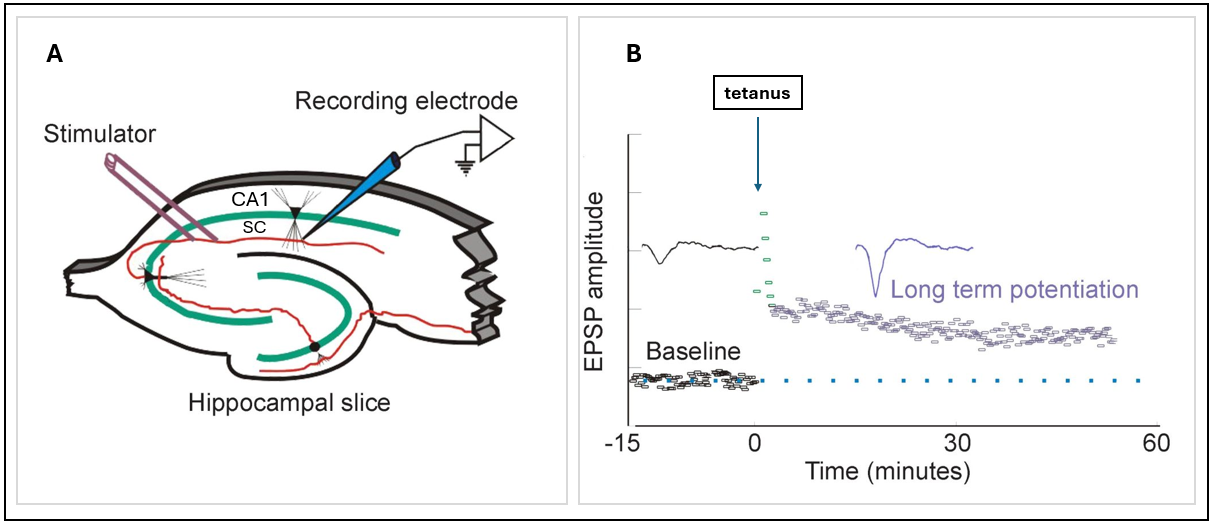
\includegraphics[width=0.7\linewidth,height=\textheight,keepaspectratio]{20-biology_figures/ltp_persistence.PNG}

}

\caption[Bliss and Lomo's experiment]{\label{fig-ltp-persistence}(A)
Bliss and Lomo's experiment
{[}\citeproc{ref-bliss1973Longlastinga}{24}{]} demonstrated LTP in the
hippocampus by stimulating the perforant pathway in an anaesthetized
rabbit. The experimental setup involved placing a stimulating electrode
in the axons of the perforant pathway at the hippocampal entry, while a
recording electrode was positioned in the CA1 region. Axonal projections
from the entorhinal cortex innervate granule cells in the dentate gyrus
(DG) via the perforant pathway. These granule cells, in turn, send their
axonal projections to pyramidal neurons in the CA3 region. The CA3
neurons then excite pyramidal neurons in the CA1 region through the
Schaffer collateral-commissural pathway (SCC), forming a critical neural
circuit for hippocampal information processing. (B) The results showed
that the high-frequency stimulation (HFS) of SCCs led to a lasting
increase in field excitatory postsynaptic potentials (fEPSP) amplitude,
further supporting the concept of LTP as a measurable and significant
phenomenon (left). The results revealed that high-frequency stimulation
(HFS) of the SCC led to a persistent increase in the amplitude of
fEPSPs, providing further evidence for LTP as a measurable and
significant phenomenon (left panel). The right panel shows LTD induced
by low-frequency stimulation (LFS). Synaptic strength is quantified as
the initial slope of the fEPSP (normalised to baseline), and this is
plotted over time. Figure adapted from
{[}\citeproc{ref-curtis2024Building}{25}{]}.}

\end{figure}%

In 1986, Morris et al.~provided some of the first evidence that LTP was
indeed required for the formation of memories \emph{in vivo} using rats
{[}\citeproc{ref-morris1986Selective}{26}{]}. These rats were trained in
the Morris water maze, a spatial memory task in which the rodents swam
in a pool of murky water until they located a platform hidden beneath
the surface. During this exercise, the rats had no other choice but to
learn the location of the hidden platform through salient cues placed at
specific positions around the maze's circumference. After the rats had
memorised where the cues and platforms were, one group was subjected to
having their hippocampi bathed in a N-methyl-D-aspartate (NMDA) receptor
blocker, while another group to whom nothing was done, served as the
control. Rats in the control group were able to locate the platform and
escape from the pool. However, the rats that had been subjected to the
blocker treatment had significantly impaired memory. Moreover, when both
groups were killed and slices of their hippocampal slices were analyzed,
LTP was readily induced in the control group, while it could not be
induced in the brains of the rats subjected to the NMDAR blocker. This
experiment using rats provided early evidence that the NMDA receptor
(and LTP) was important for at least some types of learning and memory.
In the years since, there have been many more experiments conducted on
rodents, often using fear conditioning or subjecting them to brain
injuries, that provide further evidence supporting the role of LTP in
different types of memory and learning
{[}\citeproc{ref-lynch2004LongTerm}{1}--\citeproc{ref-park2024Fear}{4}{]}.

\section{Studying synaptic plasticity at the
hippocampus}\label{studying-synaptic-plasticity-at-the-hippocampus}

The hippocampus has long been considered a key model for studying
synaptic plasticity due to its central role in learning and memory
{[}\citeproc{ref-bliss1993Synaptic}{27},
\citeproc{ref-morris2006Elements}{28}{]}. Much of this knowledge has
come from research done using rodents, often involving experiment that
induce stress or fear conditioning, and/or introduce genetic mutations
designed to impair the rodents behaviour (see the following
non-exhaustive examples:
{[}\citeproc{ref-foy1987Behavioral}{29}--\citeproc{ref-park2018Role}{33}{]}).
This brain region is particularly important in processes such as spatial
memory, episodic memory, and the consolidation of information from
short-term to long-term memory
{[}\citeproc{ref-moscovitch2016Episodic}{34},
\citeproc{ref-postle2016Chapter}{35}{]}. Its structure, which includes
well-defined neural circuits and easily identifiable synapses, makes it
an ideal system for investigating how synaptic connections change. In
particular, the CA1-CA3 regions have been extensively studied due to
their involvement in these memory processes
{[}\citeproc{ref-bliss1993Synaptic}{27},
\citeproc{ref-lisman1999Relating}{36}--\citeproc{ref-rebola2017Operation}{39}{]}.

In addition to LTP, the hippocampus also exhibits long-term depression
(LTD), a complementary mechanism in which synaptic strength is reduced
(Figure~\ref{fig-ltp-persistence})
{[}\citeproc{ref-malenka2004LTPLTDEmbarrassment}{40},
\citeproc{ref-abraham2024Longterm}{41}{]}. LTD is typically induced by
low-frequency stimulation of afferent inputs, leading to a decrease in
synaptic efficacy. This weakening of synapses is essential for synaptic
homeostasis, preventing excessive strengthening of connections and
allowing for the encoding of new information
{[}\citeproc{ref-luscher2012NMDA}{42},
\citeproc{ref-nabavi2014Engineering}{43}{]}. Together, LTP and LTD are
thought to form the basis of bidirectional synaptic plasticity, enabling
the hippocampus to modulate and refine its neural circuits to optimise
memory storage and retrieval. The focus of this thesis is on LTP to
further understand learning and memory at the cellular and molecular
level.

It is important to note here that LTP does not equal memory, though they
are linked. LTP refers to long-lasting enhancement in synaptic strength
and signal transmission between neurons. As we have just seen, it is
considered a cellular mechanism underlying learning and memory,
primarily observed in brain regions like the hippocampus, where synaptic
activity is persistently amplified in response to high-frequency
stimulation {[}\citeproc{ref-burgess2002Human}{44}{]}. Memory, on the
other hand, is a higher level process by which information is encoded,
stored, and retrieved in the brain. Memory underpins cognitive functions
and allows for the recall of past events, facts, and procedures
{[}\citeproc{ref-abraham2019Plasticity}{19}{]}; nevertheless, as we will
discuss next, synaptic strengthening and weakening provide compelling
characteristics that make LTP a prime candidate to study molecular
mechanisms underpinning memory formation.

\section{LTP as an attractive model to explain memory and
learning}\label{sec-LTP-to-explain-memory}

To this day, LTP remains a compelling model for explaining memory at the
cellular and molecular level. There are several experimental strategies
that are widely used to explore the relationship between LTP and
learning and memory. One widely used approach involves behavioural
pharmacological studies, in which the effects of drugs that inhibit LTP
induction are assessed in parallel with their impact on learning and
memory performance {[}\citeproc{ref-dringenberg2020History}{2},
\citeproc{ref-najenson2024LTP}{45}{]}. These studies often reveal that
pharmacological blockade of key molecular pathways necessary for LTP,
such as NMDAR activity or kinase signalling, is associated with deficits
in learning tasks. A well-known example is the pharmacological
inhibition of NMDARs in rats using the Morris Water Maze (see example
description in Section~\ref{sec-learning-memory-plasticity}), where
NMDAR antagonists reduce LTP and impair the acquisition of spatial
information, correlating NMDARs and LTP impairment with deficits in
spatial memory.

Another strategy involves the use of genetic manipulations, particularly
gene deletion (knockout) or transgenic mice. For example, knockout mice
lacking \(\alpha\)-CaMKII, the predominant isoform in the hippocampus,
exhibit a complete loss of LTP at Schaffer collateral synapses
{[}\citeproc{ref-stevens1994Role}{46},
\citeproc{ref-incontro2018CaMKII}{47}{]}. These mice also show severe
deficits in spatial learning. These examples illustrate that when LTP is
impaired, memory performance is also often disrupted, supporting a
correlation between the two. They also highlight the ethical
implications of such invasive experiments, which would not be morally
acceptable if conducted in humans in our current day and age, yet we
talk about these experiments as if they were normal routine to explain
molecular mechanisms of learning and memory.

The proposal of LTP as a leading model to explain learning and memory,
however, has not been one without significant challenges. Interestingly,
different studies have shown that when rats undergo nonspatial
pretraining (a technique designed to teach the rats the behavioural
strategies necessary for successfully completing the maze, without
having the rat learn a specific spatial location of the platform) before
application of an NMDAR blocker, they exhibit intact spatial learning
despite complete LTP blockade
{[}\citeproc{ref-bannerman1995Distinct}{48},
\citeproc{ref-saucier1995Spatial}{49}{]}. Suggesting that hippocampal
LTP is not strictly \emph{necessary} for spatial memory acquisition, and
that there are other mechanisms apart from LTP through which learning
and memory can proceed {[}\citeproc{ref-moser2000Pretraining}{50}{]}.

These examples highlight the complexity of these processes and start to
shed light as to why their exact molecular mechanisms remain elusive. In
fact, it is worth noting that LTP is not the sole mechanism contributing
to memory storage. Alternative mechanisms, including long-term
depression (LTD), neurogenesis, changes in neuronal excitability, and
specialized neuronal assemblies (for example engram cells), likely
interact with or compensate for LTP during learning and memory
{[}\citeproc{ref-luscher2012NMDAc}{51}--\citeproc{ref-luis2022Understanding}{54}{]}.
Nonetheless, whilst LTP is not the only mechanism underlying learning
and memory, it still provides a valuable model for understanding the
cellular and molecular processes involved.

Adding further complexity to the relationship between LTP and memory,
since its discovery, different forms of LTP have been observed across
various regions of the brain in both humans and non-human animals
{[}\citeproc{ref-chen1996Longterm}{55}--\citeproc{ref-spriggs2019Human}{58}{]}.
Moreover, the different forms of LTP further depend on a number of
factors such as developmental stage, pre- or post-synaptic stimulation
as well as stimulation protocols. Two main types of LTP have been
described as being either NMDA receptor-dependent or NMDA
receptor-independent {[}\citeproc{ref-morris1986Selective}{26},
\citeproc{ref-collingridge1983Excitatory}{59}--\citeproc{ref-kumar2011LongTerm}{72}{]}.
This project will focus on studying the NMDA receptor-dependent form of
LTP at synapses in the CA1 region of the hippocampus. To avoid
ambiguities, this is the type of LTP discussed unless otherwise stated.

\subsection{Dividing LTP into phases}\label{sec-LTP-phases}

LTP is typically divided into distinct phases: induction, expression,
and maintenance. These phases describe the progression from the initial
trigger of synaptic potentiation to the long-lasting changes in synaptic
strength {[}\citeproc{ref-sweatt2010Chaptera}{73}{]}. To provide a
clearer understanding of the molecular mechanisms underlying LTP, key
molecular interactions associated with these phases are described next.

\emph{Induction} refers to the transient events that initiate the
formation of LTP. This phase involves high-frequency (tetanic)
stimulation of presynaptic fibres, which leads to the release of
glutamate. Glutamate binds to both
\(\alpha\)-amino-3-hydroxy-5-methyl-4-isoxazolepropionic acid receptors
(AMPARs) and NMDARs on the postsynaptic membrane
{[}\citeproc{ref-scheefhals2018Functional}{74}{]}. Importantly, although
glutamate binds to NMDARs, this alone is typically insufficient to open
the channel and let ions through due to the \(\mathrm{Mg^{2+}}\) voltage
block. In contrast, AMPARs' fast kinetics and voltage independence
rapidly mediate membrane depolarisation by allowing Na⁺ influx into the
postsynaptic cell {[}\citeproc{ref-otmakhova2002PathwaySpecific}{75},
\citeproc{ref-fuenzalida2010Role}{76}{]}. If this depolarisation is
strong enough to remove the \(\mathrm{Mg^{2+}}\) block from the NMDAR
channel,\(\mathrm{Ca^{2+}}\) influx through this channel is increased,
initiating downstream signalling and setting the stage for LTP. NMDA
receptors function as molecular coincidence detectors, permitting ion
flux only when both agonist binding such as glutamate and membrane
depolarisation coincide to activate the receptors. This mechanism
ensures tight regulation of calcium entry, with elevated or reduced Ca²⁺
influx triggering LTP or LTD, respectively. This coincidence detection
permits NMDARs to facilitate spike-timing dependent plasticity, where
the precise timing between presynaptic and postsynaptic activity
dictates whether plasticity results in potentiation or depression
{[}\citeproc{ref-fuenzalida2010Role}{76}--\citeproc{ref-martinez-gallego2022Role}{79}{]}.

\emph{Expression and maintenance} refer to the phases in which the
molecular and cellular changes triggered during the induction phase are
translated into long-lasting alterations in synaptic strength. These
changes typically involve an increase in the number of receptors and
their sensitivity {[}\citeproc{ref-reymann2007Late}{80},
\citeproc{ref-abraham2008LTP}{81}{]}. For instance, phosphorylation of
AMPA receptors by proteins within the PSD enhances their ion
conductance, thereby amplifying the postsynaptic response to glutamate
{[}\citeproc{ref-sacktor2008Chapter}{82},
\citeproc{ref-purkey2020PhosphorylationDependent}{83}{]}. In addition,
synaptic structure is often modified, with dendritic spines enlarging or
new synaptic connections forming, further strengthening their connection
{[}\citeproc{ref-sala2014Dendritic}{84}--\citeproc{ref-meldolesi2022PostSynapses}{86}{]}.
Long-lasting alterations in intracellular signalling pathways, such as
enhanced activation of protein kinases also contribute to the sustained
strengthening of synaptic transmission
{[}\citeproc{ref-mayford2007Protein}{87}{]}. Structural modifications,
such as the enlargement of dendritic spines and cytoskeletal
rearrangement mediated by actin polymerisation, support the long-term
persistence of LTP. Protein synthesis, regulated by transcription
factors like CREB (cAMP response element-binding protein), also
facilitates the production of proteins necessary for synaptic
stabilisation {[}\citeproc{ref-lamprecht2004Structurala}{88}{]}.
Additionally, scaffolding proteins, such as PSD-95, \(\alpha\)-actinin-2
and more, anchor AMPA receptors at the postsynaptic density
{[}\citeproc{ref-debartolomeis2004Postsynaptic}{89},
\citeproc{ref-ivie2018ReproducibilityScientificComputing}{90}{]},
ensuring their sustained incorporation into the synaptic membrane. These
changes collectively enable the persistence of LTP, making it a robust
mechanism for memory storage at the cellular level.

Additionally, LTP is often further categorised into early-phase LTP
(E-LTP) and late-phase LTP (L-LTP), although a short term potentiation
and an intermediate phase of LTP have also been suggested
{[}\citeproc{ref-kumar2011LongTerm}{72},
\citeproc{ref-huang1998Synaptic}{91}--\citeproc{ref-lisman2005Phases}{93}{]}.
E-LTP occurs shortly after high-frequency stimulation of a synapse, and
is typically characterized by a rapid increase in synaptic strength that
lasts for a few minutes to hours. It relies primarily on the activation
of NMDARs and the influx of calcium ions
{[}\citeproc{ref-malenka1992Temporal}{94}--\citeproc{ref-bliss2018Longterm}{97}{]}.
L-LTP, on the other hand, is the prolonged phase of synaptic enhancement
that can last for days or even weeks
{[}\citeproc{ref-jackson1993Stereotypical}{98}--\citeproc{ref-mohns2008Synchronous}{103}{]}.
L-LTP is dependent on new protein synthesis and gene expression. This
phase is critical for the consolidation of memory and is associated with
structural changes in the synapse, including the growth of dendritic
spines and the synthesis of new receptors
{[}\citeproc{ref-bliss2018Longterm}{97},
\citeproc{ref-baltaci2019Molecular}{104}{]}.

The categorisation of LTP into distinct phases is not rigidly defined as
strictly sequential; rather, the phases serve as distinct categories to
help us talk about the different stages of LTP. Induction, expression,
and maintenance can apply to both E-LTP and L-LTP; with E-LTP and L-LTP
phases being \emph{induced} and \emph{expressed} in diverse ways. For
example, during E-LTP, expression can involve post-translational
modifications of existing proteins, such as phosphorylation of AMPA
receptor subunits by kinases like CaMKII or PKC, which increases
receptor conductance, whereas during L-LTP, expression often requires
protein synthesis to sustain long-term changes
{[}\citeproc{ref-abraham2008LTP}{81},
\citeproc{ref-pfeiffer2006Current}{105}{]}. These changes are then
\emph{maintained} for differing durations, from seconds or minutes in
E-LTP to hours or longer in L-LTP
{[}\citeproc{ref-abraham2003Properties}{106}{]}. Additionally, E-LTP and
L-LTP are not mutually exclusive. In fact, depending on the specific LTP
induction protocol applied, E-LTP can happen concurrently with the
development of L-LTP, with one gradually replacing the other over time
{[}\citeproc{ref-bliss1993Synaptic}{27},
\citeproc{ref-malenka2004LTPLTDEmbarrassment}{40},
\citeproc{ref-luscher2012NMDA}{42},
\citeproc{ref-roberson1996Biochemists}{107}--\citeproc{ref-nicoll2003Expression}{109}{]}.
This PhD research investigates the specific molecular interactions
between CaMKII and NMDARs, primarily focusing on their roles in E-LTP
induction and maintenance.

\subsection{Key features of NMDAR-dependent
LTP}\label{key-features-of-nmdar-dependent-ltp}

To better understand NMDAR-dependent LTP, we first examine the structure
and function of these receptors and their role in the process. NMDARs
are non-selective cationic, glutamate receptors primarily located at
dendritic spines where they links to intracellular proteins within the
postsynaptic density (PSD) through subunit-specific
interactions.{[}\citeproc{ref-volianskis2015LongtermPotentiationRole}{110}{]}.
NMDARs are heterotetramers commonly composed of two GluN1 and two GluN2
subunits (Figure~\ref{fig-NMDAR}). There are different subunit subtypes,
for example GluN2 can be found as GluN2A, GluN2B, GluN2C or GluN2D, and
we know there are GluN3A and 3B isoforms too
{[}\citeproc{ref-ciabarra1995CloningCharacterizationChi1}{111},
\citeproc{ref-kvist2013StructurebasedDiscoveryAntagonists}{112}{]}.

The specific subunit composition of NMDARs influences their properties
and functions. For example, a ``GluN2B-GluN2A developmental switch'' has
been observed in rodents
{[}\citeproc{ref-piggott19923HMK801}{113}--\citeproc{ref-mckay2018Developmental}{115}{]}
(and humans {[}\citeproc{ref-piggott19923HMK801}{113}{]}) where GluN2B
is predominantly present in the early postnatal brain, but switches to
GluN2A during early development. Eventually, GluN2A subunits become more
numerous than GluN2B. These subtypes have different kinetics, where
NMDAR with more GluN2B subunits remain open for longer compared to those
with GluN2A subunits
{[}\citeproc{ref-liu2004SwitchingNMDAReceptor}{116}{]}. In the postnatal
brain, a higher abundance of GluN2B-containing NMDARs enables greater
calcium influx and enhances synaptic plasticity. This has been suggested
to support faster learning and stronger memory formation in early
development, partly accounting for greater memory abilities in the
immediate postnatal period compared to later in life
{[}\citeproc{ref-bar-shira2015GeneExpressionSwitching}{117}{]}.

\begin{figure}[H]

\centering{

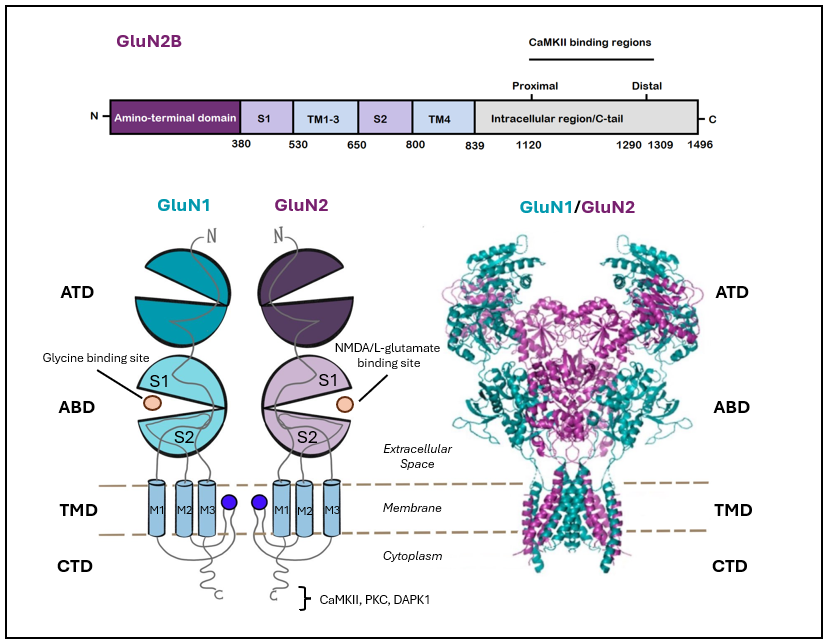
\includegraphics[width=0.9\linewidth,height=\textheight,keepaspectratio]{20-biology_figures/NMDAR.png}

}

\caption[NMDAR structure]{\label{fig-NMDAR}NMDARs are heterotetramers
composed of four subunits, typically two GluN1 and two GluN2 subunits. A
cross-sectional schematic of two subunits is shown in (A), alongside a
structural model, and a simplified pictogram of the full tetrameric
assembly is shown in (B). Each subunit has four major structural
domains: the amino-terminal domain: ATD, the agonist-binding domain:
ABD, the transmembrane domain: TMD, and the C-terminal domain: CTD. The
ATD is located extracellularly and is primarily responsible for subunit
assembly and allosteric modulation. Ligands bind to the ABD site,
glutamate binds to GluN2 subunits, while glycine binds to GluN1
subunits. Ligand binding at the ABD, together with membrane
depolarization to relieve the voltage-dependent magnesium block, is
necessary to open the ion channel. The TMD spans the cell membrane and
forms the ion channel pore. It consists of three membrane-spanning
helices: M1, M3, and M4, which collectively shape the channel's
permeability to calcium (\(\mathrm{Ca^{2+}}\)), sodium
(\(\mathrm{Na^{+}}\)), and potassium (\(\mathrm{K^{+}}\)) ions. And a
re-entrant loop, M2, which dips into the membrane from the cytoplasmic
side. The CTD is located intracellularly and serves as a platform for
binding to various intracellular proteins, including scaffolding
proteins and kinases. CaMKII binds with high affinity to the CTD of the
GluN2B subunit. Panel (C) illustrates the domain structure of a GluN2B
subunit, highlighting the location of the proximal and distal CaMKII
binding regions within the intracellular CTD region (in grey). Numbers
on the x axis represent amino acid numbers in the GluN2B subunit.
Adapted from {[}\citeproc{ref-valdivielso2020GlutamateGated}{118}{]}.}

\end{figure}%

NMDARs are primarily permeable to calcium ions and require both
glutamate and glycine as ligands, with glutamate being the more common
ligand and glycine serving as a co-agonist
{[}\citeproc{ref-traynelis2010Glutamate}{119}--\citeproc{ref-hansen2018Structure}{121}{]}.
The binding of these ligands typically does not open the channel due to
a voltage-dependent magnesium block, which is removed only once the
neuron is sufficiently depolarized
{[}\citeproc{ref-ruppersberg1994Mechanism}{122}{]}. This feature confers
to NMDARs the role of a ``coincidence detector''
{[}\citeproc{ref-seeburg1995NMDA}{123}{]}, as discussed in
Section~\ref{sec-LTP-phases}.

The binding of CaMKII to the GluN2B subunit of NMDARs is considered a
critical step in triggering structural changes in dendritic spines
following LTP induction. Compared to other subunits, CaMKII binds more
readily to GluN2B
{[}\citeproc{ref-strack1998Autophosphorylationdependent}{124}--\citeproc{ref-barria2005NMDA}{126}{]},
and this interaction appears to be a primary site involved in LTP
mechanisms {[}\citeproc{ref-barria2005NMDA}{126},
\citeproc{ref-bayer2001Interactiona}{127}{]}. Specifically, the
interaction between CaMKII and the intracellular region of the GluN2B
subunit's cytoplasmic tail (C-tail) plays a pivotal role in this
process, as further discussed in
Section~\ref{sec-CaMKII-NMDAR-association}.

LTP is a process in which the strength of synaptic connections is
enhanced, and it relies heavily on the activity of NMDARs as well as
another important glutamate receptor, namely: AMPARs. Both of these
receptors are located on the PSD
{[}\citeproc{ref-hunt2012Synaptic}{128},
\citeproc{ref-chater2014Role}{129}{]}. Although both are glutamate
receptors, they have importantly different kinetics and channel
properties.

AMPARs mediate rapid excitatory synaptic transmission, with a peak
response time of approximately 200 \(\mu\text{s}\) and decay constants
of around 2-3 ms
{[}\citeproc{ref-jonas2000Time}{130}--\citeproc{ref-choquet2010Fast}{132}{]}.
These receptors are primarily permeable to \(\mathrm{Na^{+}}\) ions and
are voltage-independent, enabling the swift influx of sodium into the
postsynaptic neuron upon synaptic transmission. In contrast, NMDARs have
a slower peak response time of approximately 10 ms and a decay constant
of around 100 ms
{[}\citeproc{ref-perouansky1993Kinetic}{133}--\citeproc{ref-tovar2017Modulating}{135}{]}.
Their ion flow is regulated by their voltage-dependent magnesium block,
which prevents ion entry at resting membrane potentials and requires
sufficient depolarization for activation. Together, AMPARs and NMDARs
work in concert to regulate synaptic plasticity. AMPARs mediate the
initial rapid response to glutamate, while NMDARs are crucial for the
longer-term changes in synaptic strength that underlie LTP (and LTD)
(Figure~\ref{fig-nmdar-ampar})
{[}\citeproc{ref-turrigiano2000Hebb}{136},
\citeproc{ref-brown2022Synaptic}{137}{]}.

\begin{figure}[H]

\centering{

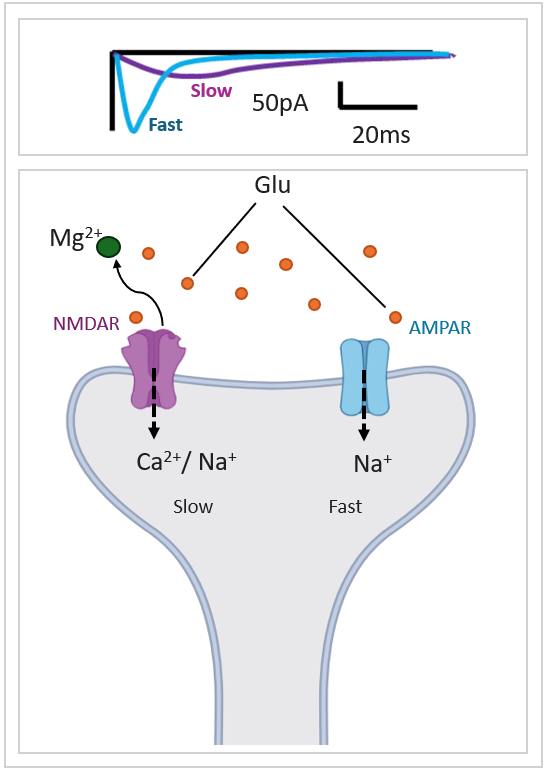
\includegraphics[width=0.5\linewidth,height=\textheight,keepaspectratio]{20-biology_figures/nmda-ampar.PNG}

}

\caption[AMPARs and NMDARs mediate fast and slow synaptic currents,
respectively]{\label{fig-nmdar-ampar}(\emph{Top}) synaptic current
traces are shown in response to glutamate receptor activation, with two
distinct kinetic components. The fast component -the blue trace-
corresponds to AMPAR-mediated currents, which activate and deactivate
rapidly. The slow component -in purple- corresponds to NMDAR-mediated
currents, which have a slower activation and deactivation profile. The
y-axis represents current amplitude in picoamperes (pA), while the
x-axis represents time in milliseconds (ms). (\emph{Bottom}) schematic
diagram of synaptic transmission, highlighting the roles of AMPARs and
NMDARs in excitatory synaptic signalling. Glutamate (Glu) can bind to
both receptor types. AMPARs, mediate fast synaptic currents by allowing
sodium ions (\(\mathrm{Na^{+}}\)) to enter the postsynaptic neuron.
NMDARs mediate slow synaptic currents, allowing both calcium
(\(\mathrm{Ca^{2+}}\)) and sodium (\(\mathrm{Na^{+}}\)) ions inside the
cell. NMDAR activation requires the removal of a magnesium
(\(\mathrm{Mg^{2+}}\)) block.}

\end{figure}%

\subsection{Molecular Signalling in LTP: Role of Calcium, CaMKII and
Phosphatases}\label{molecular-signalling-in-ltp-role-of-calcium-camkii-and-phosphatases}

A key second messenger in NMDAR-dependent LTP is calcium. This ion
drives signalling cascades through the activation of the intermediary
\(\mathrm{Ca^{2+}}\) sensitive protein calmodulin (CaM). During LTP,
elevated \(\mathrm{Ca^{2+}}\) influx activates CaM, which subsequently
triggers several kinases, such as Protein Kinase C (PKC) and
\(\mathrm{Ca^{2+}}\)-calmodulin-dependent protein kinase II (CaMKII)
{[}\citeproc{ref-gnegy2000Ca2}{138}--\citeproc{ref-mohanan2022Role}{140}{]}.
CaMKII has been shown to have several important effects during LTP.
Namely, CaMKII is one of the main kinases that phopshorylates AMPARs,
thereby elevating these receptor's channels conductance. CaMKII has also
been shown to be important for the recruitment of AMPA receptors to the
PSD following synaptic stimulation during LTP
{[}\citeproc{ref-hayashi2000Driving}{141},
\citeproc{ref-herring2016LongTerm}{142}{]}. More recently, CaMKII
binding to NMDARs has been proposed to be key for LTP induction and
maintenance at synapses in the brain
{[}\citeproc{ref-bayer2024Revised}{11}{]}.

In contrast to LTP, low levels of Ca2+ during LTD activates a cascade of
competing signalling pathways. For instance, during LTD, CaM binds to
and activates a well known phosphatase: calcineurin, also known as
Protein Phosphatase 2B (PP2B)
{[}\citeproc{ref-shibasaki2002Calcineurin}{143}{]}. Calcineurin can
dephosphorylate the GluA1 subunit of AMPARs, reversing the
phosphorylation that would normally enhance receptor activity and
membrane insertion, thereby reducing synaptic strength
{[}\citeproc{ref-kim2014Calcineurin}{144},
\citeproc{ref-zhou2024Calcineurin}{145}{]}. Other phosphatases, such as
Protein Phosphatase 1 (PP1) and PP2A play central roles in the
regulation of synaptic plasticity during both LTP and LTD. Their actions
not only depend on the relative levels of kinase and phosphatase
activity, but also help determine the direction and extent of synaptic
change. Their precise regulation ensures the appropriate strengthening
or weakening of synapses during learning and memory processes
{[}\citeproc{ref-munton2004Role}{146}--\citeproc{ref-belmeguenai2005Role}{148}{]}.

\begin{figure}

\centering{

\pandocbounded{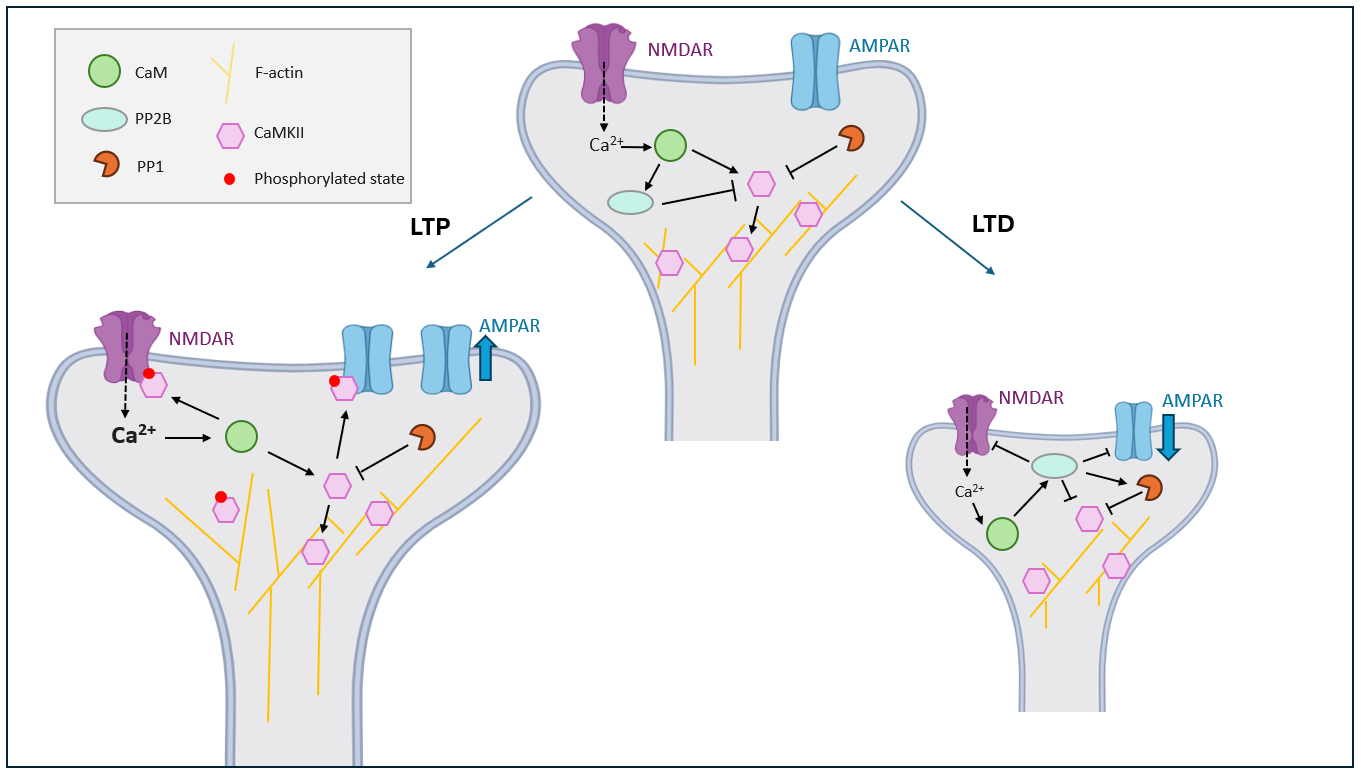
\includegraphics[keepaspectratio]{20-biology_figures/signalling_ltp_ltd.PNG}}

}

\caption[LTP and LTD pathways]{\label{fig-ltp-ltd}Molecular Signalling
in Synaptic Plasticity: CaMKII in LTP and LTD Pathways. High frequency
stimulation leads to LTP (left), characterised by a large and sustained
Ca²⁺ influx through NMDARs. This activates CaM, which in turn stimulates
CaMKII and PKC, promoting AMPAR phosphorylation and insertion into the
PSD, strengthening synaptic transmission. During LTP, CaMKII isoforms
associated to F-actin filaments separate from it and allow the dendritic
spine to grow. Low-frequency stimulation induces LTD (right), where a
smaller Ca²⁺ influx preferentially activates PP2B over CaMKII, leading
to PP1 activation and AMPAR dephosphorylation. The downregulation of
AMPARs from the synaptic membrane weakens synaptic transmission.
Additionally, reduced CaMKII dissociation from actin filaments
contributes to synaptic depression.}

\end{figure}%

The spatial and temporal dynamics of calcium influx, which vary
depending on the frequency and pattern of neuronal activity are detected
by proteins in the PSD and this triggers differing signalling cascades.
These calcium signals can lead to opposing outcomes in NMDAR-dependent
plasticity, contributing to either long-term potentiation (LTP) or
long-term depression (LTD). The precise localisation of key proteins
involved in these processes near NMDARs is thought to enable the
receptors to detect subtle spatio-temporal variations in calcium levels
and modulate downstream signalling accordingly
{[}\citeproc{ref-gladding2011Mechanisms}{149},
\citeproc{ref-brini2013Intracellular}{150}{]}. Hence, highlighting how
this PhD research is well positioned to investigate LTP mechanisms,
particularly by focusing on the spatio-temporal dynamics of NMDARs and
CaMKII. But why specifically focus on the interactions between these two
proteins?

To answer this question, we can call back on the importance of how NMDA
receptors' ability to act as a coincidence detector underpins hallmark
features of LTP. NMDARs are essential mediators for the induction of
NMDAR-dependent LTP. Indeed, inhibition of these receptors in various
regions of the hippocampus has been shown to prevent LTP induction, as
well as lead to impairments in learning and memory in rodents
{[}\citeproc{ref-morris1986Selective}{26},
\citeproc{ref-collingridge1983Excitatory}{59}{]}. Likewise, both
pharmacological inhibition and genetic knockout of NMDARs subunits have
been shown to block LTP induction in rodent hippocampal circuits
{[}\citeproc{ref-luscher2012NMDA}{42},
\citeproc{ref-hunt2012Synaptic}{128},
\citeproc{ref-alkadhi2021NMDA}{151}{]}. Moreover, over the past few
decades, CaMKII has emerged as a critical molecule in the study of
synaptic plasticity, with substantial evidence supporting its role as a
key mediator of LTP {[}\citeproc{ref-sanhueza2013CaMKII}{9},
\citeproc{ref-lisman2012MechanismsCaMKIIAction}{152}--\citeproc{ref-chen2024CaMKII}{155}{]}.
In particular, its structural interaction with NMDARs seems to be a
critical and minimal requirement for the induction of LTP, as we will
see in the following Section~\ref{sec-camkii-properties}.

\section{Biophysical properties of CaMKII}\label{sec-camkii-properties}

CaMKII is expressed ubiquitously in animals, with four known isoforms
\(\alpha\), \(\beta\), \(\gamma\) and \(\lambda\)
{[}\citeproc{ref-zalcman2018CaMKIIa}{156},
\citeproc{ref-tullis2023Distinct}{157}{]}. This study focuses on the
brain specific \(\alpha\) isoform, which constitutes up to 2\% of total
brain protein {[}\citeproc{ref-lisman2012MechanismsCaMKIIAction}{152},
\citeproc{ref-kennedy1983Biochemical}{158},
\citeproc{ref-chen2005Mass}{159}{]}. \(\alpha\)-CaMKII is one of the
main proteins in the PSD, and has extensively been shown to be important
for LTP and memory formation {[}\citeproc{ref-hell2014CaMKII}{160},
\citeproc{ref-yasuda2022CaMKIIc}{161}{]}. Unless otherwise stated,
references to CaMKII throughout this project will specifically pertain
to \(\alpha\)-CaMKII. This kinase is a large holoenzyme consisting of 10
to 12 (and sometimes 14) subunits
{[}\citeproc{ref-rosenberg2005StructureAutoinhibitedKinase}{162}--\citeproc{ref-buonarati2021Conserved}{165}{]}.
CaMKII holoenzymes are made up of two hexameric rings stacked together,
where the association domain (or hub) holds the subunits together in a
double-ring formation (Figure~\ref{fig-CAMKII} (B)).

Each of the subunits has a N-terminal catalytic/kinase domain (dark blue
section Figure~\ref{fig-CAMKII}), followed by a regulatory domain that
contains a self-inhibitory region and a binding site for the
Ca2+/calmodulin complex (green and pink in Figure~\ref{fig-CAMKII}), the
variable linker domain (grey section in Figure~\ref{fig-CAMKII}) and the
C-terminal hub domain (light blue Figure~\ref{fig-CAMKII}). The kinase
domain is the region that binds substrates and contains the ATP-binding
site necessary for phosphorylation
{[}\citeproc{ref-pellicena2014CaMKII}{166}{]}. There is also a model
proposed where CaMKII subunits have an S-site and T-site within the
kinase domain where the GluN2B subunit of NMDARs binds to
{[}\citeproc{ref-strack2000Mechanisma}{167},
\citeproc{ref-bayer2001Interaction}{168}{]}, although this has recently
been contested {[}\citeproc{ref-ozden2022CaMKII}{169}{]}, as discussed
in Section~\ref{sec-CaMKII-NMDAR-association}.

\begin{figure}[H]

\centering{

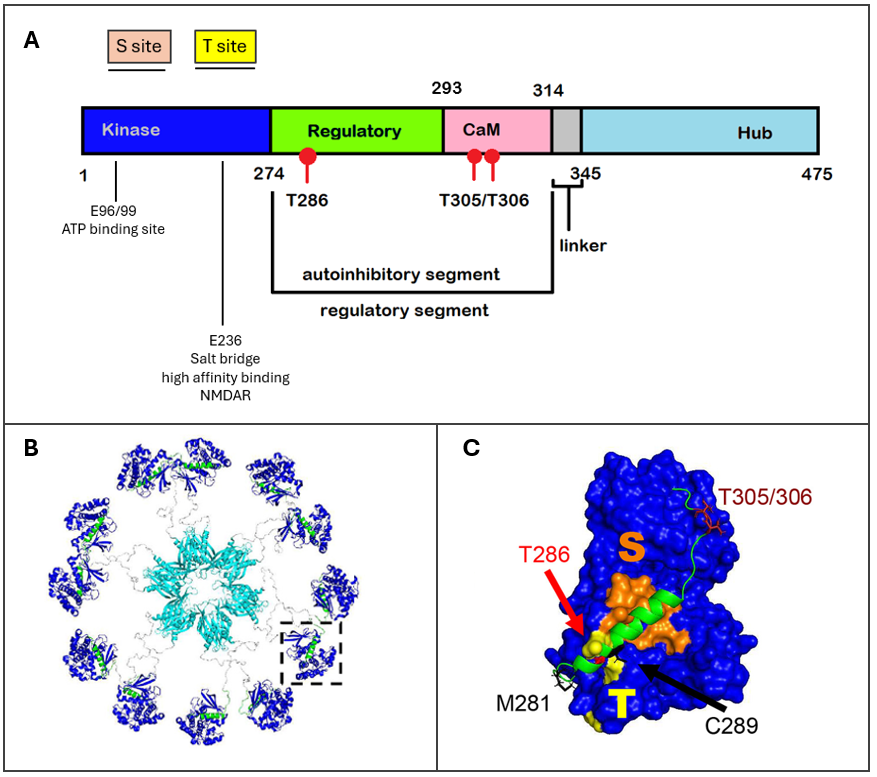
\includegraphics[width=0.8\linewidth,height=\textheight,keepaspectratio]{20-biology_figures/CAMKII.PNG}

}

\caption[Schematic representation of CaMKII]{\label{fig-CAMKII}(A)
Schematic representation of CaMKII, highlighting key domains,
phosphorylation Threonine (T) sites (T286, T305/306), and regulatory
regions. (B) Holoenzyme structure crystallography showing dodecameric
assembly, view from above, rigs are stacked on top of each other
{[}\citeproc{ref-myers2017CaMKII}{164}{]}. The structure is based on the
crystal structure available at the Protein Data Bank (PDB: 5U6Y). (C) A
single subunit, with a close up of the kinase domain with
phosphorylation sites (T286, T305/306) and proposed substrate-binding
sites S-site (orange) and T-site (yellow). (\(\alpha\)-CaMKII amino
acids 7--274, PDB: 6vzk, and regulatory ribbon amino acids 281--309,
PDB: 5u6y). Figure adapted from
{[}\citeproc{ref-brown2024Studyinga}{170}{]}.}

\end{figure}%

CaMKII subunits can be found docked (also known as ``compact state''),
or undocked (or extended); and open, or closed
{[}\citeproc{ref-hoffman2011Conformational}{171},
\citeproc{ref-bhattacharyya2020Structurala}{172}{]}. The docked/undocked
states describe the compact or extended structure configurations of the
CaMKII holoenzyme subunits, where the kinase domains are packed close to
the central hub or not. The closed/open states refer to the
conformational changes in the kinase and regulatory domains; these
domains can adopt an ``open'' state, allowing kinase activity, or a
``closed'' state, in which the kinase and regulatory domain are bound
together, reducing CaMKII's kinase activity
{[}\citeproc{ref-nguyen2015Covert}{173}--\citeproc{ref-ozden2022CaMKIIb}{176}{]}
(Figure~\ref{fig-docked-undocked})(Figure~\ref{fig-CAMKII})(Figure~\ref{fig-open-close}).

In the docked state, CaMKII subunits adopt a more compact configuration,
where the regulatory domain is closely associated with the hub domain
(Figure~\ref{fig-CAMKII}). When CaMKII subunits are found in the docked
state, they cannot autophosphorylate their neighbouring subunits, even
if the subunits are open. This is because the compact shape does not
allow the kinase domain of one subunit to structurally reach its
neighbour
{[}\citeproc{ref-rosenberg2005StructureAutoinhibitedKinase}{162}{]}.
Therefore, it is thought that for CaMKII to have autophosphorylation
activity, subunits need to be in an ``open'' and undocked conformation.
Subunits in a docked, open state lack the structural capacity for
autophosphorylation activity {[}\citeproc{ref-chao2011Mechanismb}{163},
\citeproc{ref-myers2017CaMKII}{164}{]}. In the undocked state, the
regulatory domain is extended and separated from the hub domain. This
conformation makes the subunits less compact and more ``loose'' which
can facilitate interactions between subunits, and with other substrates.
When undocked, CaMKII subunits can phosphorylate neighbours so long as
they are in an open state as the kinase domain is structurally available
to perform such function. If a subunit is undocked but closed, it lacks
catalytic activity because its regulatory domain is bound to its
catalytic site, preventing the kinase domain from being accessed or
accessing targets {[}\citeproc{ref-nguyen2015Covert}{173},
\citeproc{ref-chao2011Mechanism}{177}{]}.

\begin{figure}[H]

\centering{

\pandocbounded{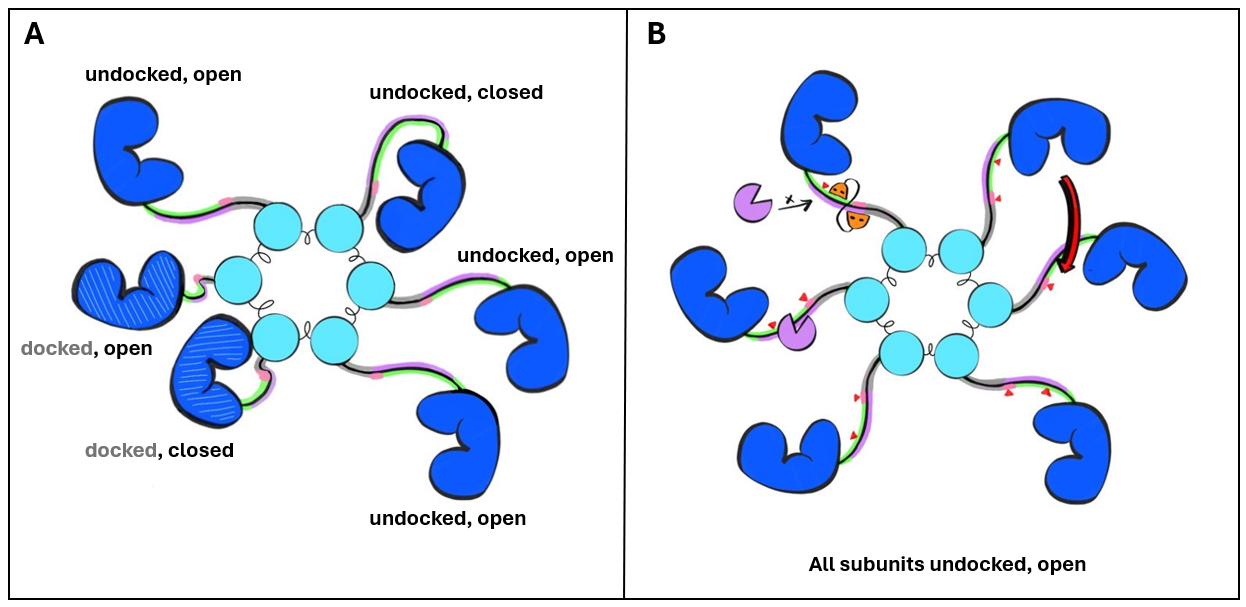
\includegraphics[keepaspectratio]{20-biology_figures/camkii_docked_undocked.PNG}}

}

\caption[CaMKII docking and undocking]{\label{fig-docked-undocked}(A)
CaMKII subunits can exist in docked (compact) or undocked (extended)
positions, and in open or closed conformations. The docked/undocked
distinction refers to the spatial arrangement of the kinase domains
(dark blue) relative to the central hub (light cyan blue), either
closely packed or extended outward. In contrast, the open/closed states
describe the structural relationship between the kinase domain (dark
blue) and regulatory (green, purple, grey) domain. In the open state,
these domains are separated, enabling kinase activity; in the closed
state, they are bound together, limiting activity. We illustrates two
docked subunits, one in an open and one in a closed conformation,
positioned near the hub. The remaining subunits are undocked, with one
shown in the closed state. (B) All subunits are shown in the undocked
and open state, with various possible interactions highlighted. When two
neighbouring subunits are both open, one can phosphorylate the other at
T286 (red arrow). A phosphatase (purple molecule) can access and
dephosphorylate T286 and/or T306 sites if the subunit is undocked and
open. However, when calmodulin (orange double-headed molecule) is bound,
the phosphorylation sites are inaccessible to the phosphatase. CaM can
bind to a subunit that is open and not phosphorylated at T306.}

\end{figure}%

\subsection{CaM binding and T286
phosphorylation}\label{sec-cam-binding-and-t286-p}

When CaMKII is in its closed conformation, structural constraints
prevent CaM from interacting with the kinase
{[}\citeproc{ref-hoffman2011Conformational}{171},
\citeproc{ref-singla2001Molecular}{178},
\citeproc{ref-gaertner2004Comparative}{179}{]}. In contrast, when CaMKII
subunits are in the open state, the calmodulin binding site of the
regulatory segment becomes available for interaction
{[}\citeproc{ref-nguyen2015Covert}{173},
\citeproc{ref-chao2011Mechanism}{177},
\citeproc{ref-gaertner2004Comparative}{179}--\citeproc{ref-asciutto2021Physical}{181}{]}.
In the open conformation, CaMKII subunits can also autophosphorylate
each other at threonine 286 (T286) found in the regulatory segment,
which prevents the segment from closing, and uncovers the binding sites
in the kinase domain for CaMKIIs substrates and anchoring proteins. In
other words, when subunits are in their open conformation, two main
events can stabilise this conformation: CaM binding to the regulatory
domain (because it prevents closing) and phosphorylation at T286 (which
is close to the hinge connecting the active domain and regulatory
domain).

Calmodulin binding is thought to stabilise CaMKII's subunits in their
open conformation, facilitating further autophosphorylation among
neighbouring subunits. What is more, binding of Ca2+/CaM has been shown
to significantly increase the kinase's affinity for
\(\mathrm{Ca^{2+}}\)/CaM itself
{[}\citeproc{ref-meyer1992Calmodulin}{182},
\citeproc{ref-putkey1996Peptide}{183}{]}, creating a feedforward loop.
This means that as more CaM binds, it makes it easier for additional CaM
to bind, which promotes further autophosphorylation and stabilisation of
the kinase in its open conformation
{[}\citeproc{ref-nguyen2015Covert}{173},
\citeproc{ref-chao2011Mechanism}{177}{]}. This phenomenon, known as CaM
trapping, refers to the increased retention of calcium bound CaM by
CaMKII following T286 autophosphorylation, which effectively locks CaM
in place even after intracellular calcium levels drop
{[}\citeproc{ref-meyer1992Calmodulin}{182},
\citeproc{ref-singla2001Moleculara}{184}{]}.

\begin{figure}[H]

\centering{

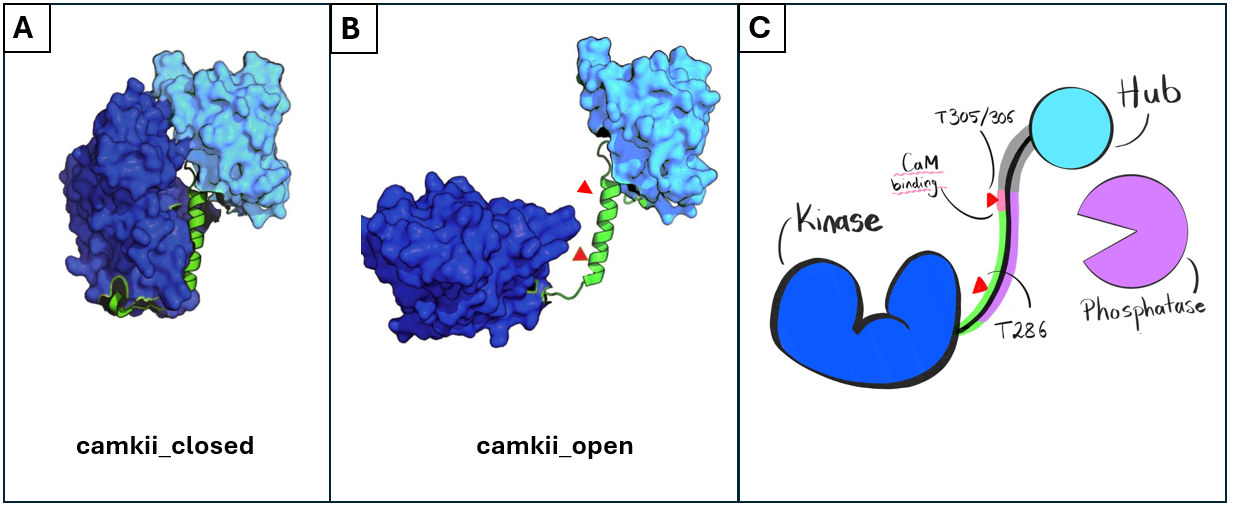
\includegraphics[width=0.7\linewidth,height=\textheight,keepaspectratio]{20-biology_figures/camkii_kinase_domain.PNG}

}

\caption[CaMKII subunit opening and closing]{\label{fig-open-close}(A-B)
Conformational states of CaMKII: closed and open with exposed
phosphorylation sites. (C) Different binding and phosphorylation sites
highlighted, CaMKII subunit in open conformation. CaM binding region and
T305/306 sites overlap; T305/306 phosphorylation prevents CaM binding.
Phosphatase can dephosphorylate both phosphorylation sites. Figure
modified from {[}\citeproc{ref-pharris2019Multistate}{185}{]}}

\end{figure}%

Furthermore, as autophosphorylation at T286 prevents the regulatory
domain from re-associating with the catalytic domain, even in the
absence of CaM, it enables CaMKII activity that is independent of
calcium. Therefore, CaMKII's increased autophosphorylation capability
allows it to retain an \emph{autonomous activity}, indepedent of
calcium/calmodulin binding, even after the initial calcium signal has
faded {[}\citeproc{ref-chang2017CaMKII}{153},
\citeproc{ref-braun1995Multifunctional}{186}--\citeproc{ref-buard2010CaMKII}{189}{]}.
This autonomous activation is thought to be important for memory
formation and synaptic modification, as it allows CaMKII to sustain
long-term changes in cellular activity, ensuring that modifications are
maintained over time. T286 autophosphorylation and CaM trapping play a
crucial role in conferring frequency-dependent activation of CaMKII
(Figure~\ref{fig-freq_detector}). Experimental studies with purified
CaMKII have shown that the enzyme responds differently to varying
frequencies and durations of Ca²⁺ spikes
{[}\citeproc{ref-chang2017CaMKII}{153},
\citeproc{ref-dekoninck1998Sensitivity}{190},
\citeproc{ref-bayer2002Alternative}{191}{]}. This frequency dependence
is thought to correlate with the requirements for LTP induction, which
is promoted by HFS and relies on CaMKII autonomy.

\begin{figure}

\centering{

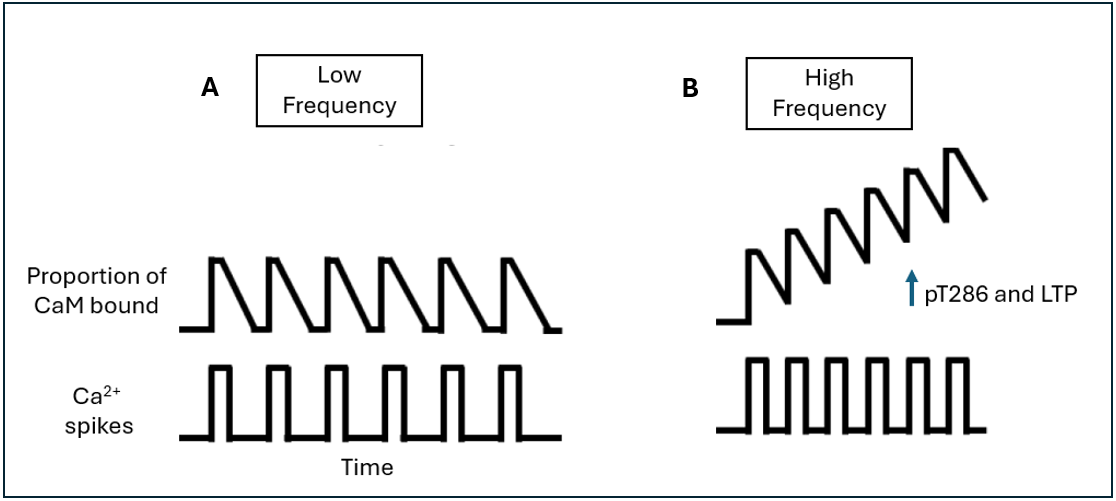
\includegraphics[width=0.7\linewidth,height=\textheight,keepaspectratio]{20-biology_figures/freq_detector.PNG}

}

\caption[CaMKII frequency detection]{\label{fig-freq_detector}The dual
role of CaM and T286 phosphorylation enables frequency detection of
threshold to induce autonomous activity. (A) At low frequency calcium
spikes, Ca2+/CaM can bind to CaMKII and dissociate between intervals.
(B) At higher stimulation frequencies, when the interval between calcium
spikes is shorter than the Ca2+/CaM dissociation time, new Ca2+/CaM
molecules can bind to neighboring CaMKII subunits before the previously
bound Ca2+/CaM fully dissociates. Adapted from
{[}\citeproc{ref-coultrap2012CaMKII}{192}{]}.}

\end{figure}%

In the literature, the term `CaMKII activity' can sometimes be used
interchangeably when referring to CaMKII subunits being in their open
state {[}\citeproc{ref-pharris2019Multistate}{185},
\citeproc{ref-nicoll2005Synaptic}{193}{]}, being bound to CaM
{[}\citeproc{ref-rellos2010Structureb}{180},
\citeproc{ref-nicoll2005Synaptic}{193}{]}, and/or being phosphorylated,
typically at the T286 site
{[}\citeproc{ref-lisman2012MechanismsCaMKIIAction}{152},
\citeproc{ref-rellos2010Structureb}{180},
\citeproc{ref-nicoll2005Synaptic}{193}{]}. However, these states are
distinct and we therefore clarify that we define different types of
activity. CaMKII can have enzymatic activity, which refers to the
protein's ability to catalyse the phosphorylation of downstream
substrates. We use the term autonomous activity, where CaMKII remains
open even after CaM dissociates. While autonomous activity still entails
enzymatic function, this distinction helps clarify whether CaMKII is
active in the presence or absence of CaM.

Furthermore, CaM binding is commonly considered to induce activation
{[}\citeproc{ref-yasuda2022CaMKIIc}{161},
\citeproc{ref-hoffman2011Conformational}{171}{]}, further obfuscating
the meaning behind CaM binding and CaMKII activation. However, studies
have demonstrated that CaMKII can exhibit enzymatic activity even in the
absence of CaM-induced activation, albeit at a reduced level
{[}\citeproc{ref-bhattacharyya2020Flexible}{175},
\citeproc{ref-rellos2010Structureb}{180},
\citeproc{ref-erickson2008Dynamic}{194}{]}, which challenges the notion
that CaM binding is synonymous with CaMKII activation.

This leads to the discussion of an `induced fit' model versus a
`conformational selection' model. In the former, an activator binds to
the enzyme and induces a conformational change. For instance, CaM
binding facilitates the opening of the CaMKII subunit. In contrast, a
`conformational selection' model suggests that the enzyme can exist in
both active and inactive conformations independently, with the activator
selectively binding to and stabilizing the active conformation, without
\emph{inducing} a conformational change. Moreover, within cells,
signaling cascades and events do not occur in a sequential, orderly
fashion; rather, they happen simultaneously, with random events
occurring at various locations and times. Therefore, in this
dissertation, the conformational selection approach is considered more
appropriate to describe the interaction leading to CaMKII activation.

\subsection{CaMKII T305/306 phosphorylation}\label{sec-t305-p}

Phosphorylation also occurs at two additional threonine residues, T305
and T306, which are thought to provide CaMKII with important
autoregulatory functions. Although their exact functions and mechanisms
are not fully understood. It has been shown that following T286
phosphorylation, this site can become phosphorylated shortly after
either by an adjacent subunit within the holoenzyme (same as for T286,
as shown in Figure~\ref{fig-docked-undocked}), or if the subunit has not
been phosphorylated at T286 (which binds at the hinge and keeps the
kinase domain ``locked'' in an open conformation), the kinase domain can
bend around via the flexible linker and access its own regulatory
segment, where T305 and T306 are located
{[}\citeproc{ref-bhattacharyya2020Flexible}{175},
\citeproc{ref-hanson1992Inhibitory}{195},
\citeproc{ref-pi2010Autonomousa}{196}{]}.

Located within the CaM binding segment, phosphorylation of the T305/306
site prevents CaM from binding to the enzyme. Similarly, if CaM is
bound, these sites cannot undergo phosphorylation
{[}\citeproc{ref-hanson1992Inhibitory}{195},
\citeproc{ref-colbran1993Inactivation}{197}{]}. Unlike T286
phosphorylation, phosphorylation at T305/306 does not prevent CaMKII
subunits from closing {[}\citeproc{ref-cook2021CaMKIIb}{198}{]}. This,
together with the fact that it prevents CaM from binding, increases the
likelihood that T305/306 phosphorylated subunits adopt the closed state
(as it reduces likelihood of CaM trapping described above). In the
closed state, the kinase's catalytic activity is reduced, as the kinase
domain is inaccessible. Therefore, T305/306 phosphorylation is often
described as reducing CaMKII's catalytic activity, or being an
``inhibitory phosphorylation''
{[}\citeproc{ref-chang2019Mechanisms}{199},
\citeproc{ref-yasuda2022CaMKII}{200}{]}. Phosphorylation at T305/306 has
been proposed to act as a form of kinetic proofreading, ensuring CaMKII
remains inactive or less active unless sustained or repetitive calcium
signals are present. This mechanism would prevent premature or excessive
kinase activation, enhancing the specificity and fidelity of
CaMKII-mediated signalling in response to synaptic activity
{[}\citeproc{ref-bayer2024Revised}{11},
\citeproc{ref-cook2021CaMKIIb}{198},
\citeproc{ref-ordyan2020Interactionsb}{201}{]}.

\subsection{CaMKII association with NMDARs: enzymatic vs structural
roles in LTP}\label{sec-CaMKII-NMDAR-association}

One of the most popular theories for memory in molecular neuroscience
has been that LTP induction (and potentially maintenance) requires
enzymatic activity of CaMKII
{[}\citeproc{ref-lisman2012MechanismsCaMKIIAction}{152},
\citeproc{ref-chang2017CaMKII}{153},
\citeproc{ref-buard2010CaMKII}{189},
\citeproc{ref-cook2021CaMKIIb}{198},
\citeproc{ref-coultrap2014Autonomous}{202}{]}. The enzymatic action of
CaMKII has two types of targets. First, itself, as T286
autophosphorylation maintains the enzyme in the open and autonomous,
conformation. Secondly, CaMKIIs enzymatic action also targets the
phosphorylation of various downstream target proteins, such as the GluA1
subunit of AMPARs, or the GluN2B subunit of NMDARs, among others
{[}\citeproc{ref-nicoll2023Synaptic}{203}{]}. Although not the focus of
this study, it is worth noting that CaMKII can enhance synaptic strength
by phosphorylating AMPAR subunits such as GluA1, increasing their
conductance and contributing to larger excitatory postsynaptic currents
(EPSCs). This activity also facilitates further calcium entry via
NMDARs, supporting LTP induction. In addition, it is also proposed that
\(\alpha\) and \(\beta\) CaMKII isoforms activation and their
postsynaptic translocation induces the synaptic trapping of AMPARs
diffusing in the membrane, although the exact mechanisms remain unclear
{[}\citeproc{ref-hell2014CaMKII}{160},
\citeproc{ref-diaz-alonsoLongterm}{204}--\citeproc{ref-patriarchi2018Postsynaptic}{206}{]}.

The role of T286 phosphorylation in CaMKII activity and LTP has long
been debated. Historically, T286 autophosphorylation was thought to be
essential for LTP induction, as early studies showed that T286A mutant
mice, unable to phosphorylate at this site, showed impaired LTP
{[}\citeproc{ref-giese1998Autophosphorylation}{207}--\citeproc{ref-vigil2016CaMKII}{209}{]}.
However, these conclusions were based on correlation rather than
causation. The mutation's effects could stem from CaMKII failing to
activate through alternative mechanisms, rather than proving an absolute
requirement for phosphorylation. For example, T286A CaMKII mutants have
also been shown to have reduced GluN2B binding, which is likely to be
accounting for CaMKII's disrupted function
{[}\citeproc{ref-giese1998Autophosphorylation}{207},
\citeproc{ref-gustin2011Loss}{210}{]}. A T286A mutation alone does not
isolate the effects of T286 phosphorylation from confounding factors,
such as disrupted binding or altered localisation of CaMKII.

Recent work by {[}\citeproc{ref-rumian2024LTP}{211}{]} have shed light
into this using hippocampal slices from T286A mutant mice. Since T286A
CaMKII cannot phosphorylate at T286, any LTP observed in these mutants
must occur via a mechanism independent of T286 phosphorylation.
Remarkably, high-frequency stimulation still induced LTP in T286A slices
when the ATP-competitive CaMKII inhibitor AS283 was applied. This
finding shows that T286 phosphorylation is indeed not necessary for LTP
induction. Furthermore, since AS283 inhibits CaMKII enzymatic activity,
this study also shows that enzymatic activity is not required for LTP
induction. What is more, using AS283 could reverse LTP if applied
shortly after induction, whereas applying the same inhibitor 15 minutes
later had no effects on LTP. Suggesting that CaMKII's enzymatic activity
is important during the early post-induction phase but not for later
maintenance of LTP {[}\citeproc{ref-bayer2024Revised}{11},
\citeproc{ref-rumian2024LTP}{211}{]}. It is important to note that AS283
is an experimental tool not present under physiological conditions.
While these findings demonstrate that LTP can occur without T286
phosphorylation or enzymatic activity when AS283 is used, the relevance
of this mechanism to \emph{in vivo} systems remains uncertain. The
results clearly point to a non-enzymatic role for CaMKII in LTP, but the
precise nature of that role requires further investigation.

The relative significance of CaMKIIs T286 autophosphorylation,
phosphorylation and binding of downstream target proteins, continues to
be a subjet of intense debate {[}\citeproc{ref-chang2017CaMKII}{153},
\citeproc{ref-buard2010CaMKII}{189},
\citeproc{ref-sanhueza2011Role}{212},
\citeproc{ref-cook2022CaMKIIb}{213}{]}. Much of the uncertainty in
interpreting studies that inhibit CaMKII enzymatic activity and its
exact role in LTP arises from the fact that some CaMKII enzymatic
inhibitors also affect CaMKII's structural functions, particularly its
binding to the GluN2B subunit of NMDA receptors.

In this context, at the turn of the century, research by
{[}\citeproc{ref-bayer2001Interactiona}{127}{]} demonstrated that the
binding of GluN2B and CaMKII could induce autonomous CaMKII activity.
The proposed mechanism for CaMKII and NMDAR binding was that the CTD of
the NMDAR, which has homology to CaMKIIs regulatory segment, binds to
the kinase domain in its place (Figure~\ref{fig-nmdar-binding}). This
idea presents a paradox: as binding of the regulatory domain to the
kinase domain is typically known to inhibit the kinase, rendering it
inactive/closed. Thus, with this explanation, it would be expected that
the GluN2B CTD would inhibit the kinase rather than keep it persistently
active. A long-standing proposed mechanism to explain how the CTD
peptide can keep CaMKII in its constitutive active state, is that one
end of the GluN2B CTD may act as a wedge at the T site of the CaMKII
subunit, preventing the autoinhibitory segment from reassociating, while
the other end remains loosely bound to the active S site, allowing
substrates to interact with the kinase domain
{[}\citeproc{ref-bayer2001Interaction}{168},
\citeproc{ref-nicoll2023Synaptic}{203},
\citeproc{ref-bayer2006Transitionb}{214}{]}.

However, recent crystal structure studies of CaMKII subunits challenge
this two-site-binding model, and show that CaMKII substrates, including
GluN2B among other activator petptides, bind to a single continuous site
across the kinase domain {[}\citeproc{ref-ozden2022CaMKIIb}{176}{]}.
This finding highlights a salt bridge interaction, located far from the
active S site, that enhances the binding affinity of CaMKII for
activator peptides such as GluN2B. These high-affinity interactions are
believed to sustain CaMKII's enzymatic activity by keeping the subunits
in an open, active conformation. But how, as we face the same paradox as
before? {[}\citeproc{ref-ozden2022CaMKIIb}{176}{]} propose that that
GluN2B binding is able to maintain CaMKII subunits in their open
conformation by displacing the regulatory segment, triggering a
conformational change that causes the \(\alpha\)-D helix, a structural
feature within the kinase domain, to rotate outward. This outward shift
stabilises the kinase in its active form, preventing the regulatory
segment from reassociating and allowing CaMKII to remain catalytically
active.

\begin{figure}[H]

\centering{

\pandocbounded{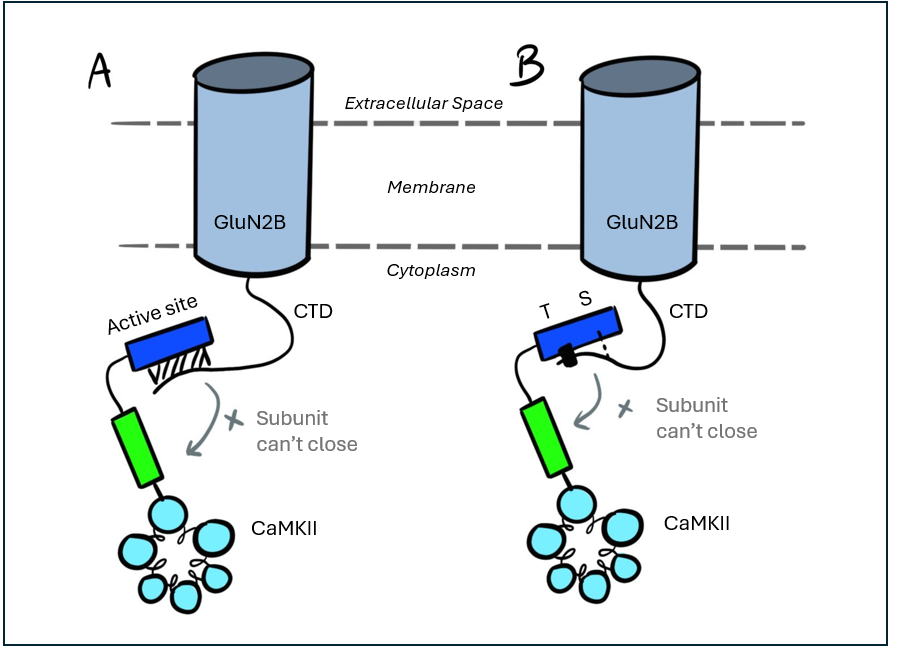
\includegraphics[keepaspectratio]{20-biology_figures/nmdar-binding.PNG}}

}

\caption[CaMKII binding to the NMDAR
GluN2B]{\label{fig-nmdar-binding}Schematic of two proposed models of
CaMKII binding to the GluN2B subunit of NMDARs. Both models propose that
CaMKII regulatory segment binds to the C-terminal domain (CTD) of
GluN2B, stabilizing CaMKII subunits in an open, active conformation.
\textbf{Model A} proposes that GluN2B binds to a single continuous site
across the CaMKII kinase domain (blue). This interaction prevents
autoinhibitory segment (green) from reassociating. This model proposes
that kinase activity is preserved via a conformational change in the
\(\alpha\)-D helix of the kinase domain (not shown), causing it to
rotate outward and accommodate binding of other substrates (not shown).
\textbf{Model B} suggests that the CaMKII kinase domain binds more
strongly at a defined T site and more weakly at a secondary S site. This
configuration may prevent the autoinhibitory segment from reassociating,
while still allowing substrate access at the active site.}

\end{figure}%

Although the exact mechanism by which CaMKII and NMDAR bind to form a
complex is not yet fully understood, existing evidence consistently
indicates that CaMKII subunits interact with the CTD of NMDARs, and that
this structural complex plays a crucial role in LTP
{[}\citeproc{ref-incontro2018CaMKII}{47},
\citeproc{ref-engelhardt2008Contribution}{215}--\citeproc{ref-foster2010Distinct}{217}{]}.
In fact, there is increasing evidence supporting a structural model in
which LTP is maintained through the binding of CaMKII to the GluN2B
subunit, independent of CaMKII's enzymatic activity
{[}\citeproc{ref-sanhueza2011Role}{212}{]}.
{[}\citeproc{ref-halt2012CaMKIIc}{218}{]} showed that disrupting
CaMKII-GluN2B binding using peptides that block this interaction such as
CN21, prevented LTP even when CaMKII kinase activity was intact. More
recently, there have been some key studies
{[}\citeproc{ref-ozden2022CaMKII}{169},
\citeproc{ref-tullis2023LTP}{219}{]} that focused on finding the minimal
requirements for the ability of CaMKII to enhance synaptic transmission
and its role in LTP maintenance. Although these studies were conducted
independently, they both arrived at a similar conclusion: the role of
T286 phosphorylation in CaMKII during LTP may not be primarily
enzymatic.

Instead, it may serve to enable and stabilize the CaMKII-GluN2B complex
that is \emph{essential} for regulating synaptic CaMKII accumulation and
supporting the associated structural functions of CaMKII required for
LTP. In other words, T286 phosphorylation modulates (not mediates) the
initial signal processing that triggers LTP induction, enabling a
downstream response via CaMKII's structural functions without requiring
enzymatic activity. It is these structural functions of CaMKII that are,
therefore, more likely to meet the essential and minimum molecular
requirements for LTP induction and maintenance
{[}\citeproc{ref-ozden2022CaMKII}{169},
\citeproc{ref-kim2016Interplay}{220}{]}, though the precise mechanisms
remain unclear. The CaMKII/NMDAR complex may enable activity-dependent
CaMKII incorporation into postsynaptic sites, potentially acting as a
structural seed to recruit postsynaptic density proteins, contributing
to synapse restructuring and plasticity.

In addition to forming a complex with GluN2B, CaMKII can phosphorylate
the S1303 site at the GluN2B CTD. However, while the CaMKII/NMDAR
binding complex is likely essential for synaptic function during LTP,
S1303 phosphorylation does not appear to be necessary
{[}\citeproc{ref-lisman2012Mechanisms}{221},
\citeproc{ref-goodell2017DAPK1}{222},
\citeproc{ref-goodell2017DAPK1}{222},
\citeproc{ref-tullis2021GluN2B}{223}{]}. Recent mutagenesis studies
detected increased S1303 phosphorylation after induced chemical LTD, but
not after LTP, suggesting that S1303 phosphorylation may be more
relevant to synaptic weakening rather than strengthening
{[}\citeproc{ref-tullis2023Distinct}{157},
\citeproc{ref-tullis2021GluN2B}{223}{]}. It is known that CaMKII and
death-associated protein kinase 1 (DAPK1), another kinase of the CaMK
family, competes for binding to the GluN2B subunit of NMDARs
{[}\citeproc{ref-goodell2017DAPK1}{222},
\citeproc{ref-goodell2017DAPK1}{222}{]}. Recently, it has been posited
that S1303 may act as a point of convergence for these kinases to
modulate GluN2B-containing NMDARs. S1303 phosphorylation may play a more
critical role in LTD, as DAPK1, which inhibits CaMKII binding, targets
this site and initiates the molecular cascade leading to LTD. In
summary, the precise mechanism of CaMKII binding to the NMDAR CTD
remains unclear. And while it is known that CaMKII can phosphorylate
S1303 in the NMDAR, this phosphorylation function remains enigmatic; the
primary function of CaMKII binding to the receptor seems to be mainly
structural during LTP {[}\citeproc{ref-tullis2021GluN2B}{223}{]}.

Phosphorylation at T305/306, unlike T286, has been more readily observed
during LTD {[}\citeproc{ref-pi2010Autonomousa}{196},
\citeproc{ref-coultrap2014Autonomous}{202}{]}; what is more,
phosphorylation at T305/306 is suggested to direct the signalling
cascade toward LTD {[}\citeproc{ref-bayer2024Revised}{11}{]}, although
the exact mechanisms remain unclear. Specifically, phosphorylation at
these sites seems to be important when CaMKII binds to GluN2B of NMDARs.
Some studies suggest that phosphorylation at these sites inhibits
binding to GluN2B {[}\citeproc{ref-elgersma2002Inhibitory}{224},
\citeproc{ref-cook2021CaMKII}{225}{]}, while others propose that binding
to GluN2B suppresses T305/306 phosphorylation
{[}\citeproc{ref-bayer2001Interaction}{168}{]}. Interestingly,
{[}\citeproc{ref-barcomb2014Autonomous}{226}{]} demonstrated that a
phosphomimic T305/306D CaMKII mutant retained its ability to bind GluN2B
without significant reduction. This finding suggests that T305/306
phosphorylated CaMKII can still bind to GluN2B, challenging the idea
that T305/306 phosphorylation directly inhibits binding, and that indeed
CaMKII can bind to GluN2B and phosphorylate at T305/306 at the same
time.

If phosphorylation at T305/306 makes CaMKII more likely to be in a
``closed'' state (see Section~\ref{sec-t305-p}), this would reduce its
likelihood of binding to GluN2B. In other words, it is not the
phosphorylation itself that directly inhibits binding, but rather that
the kinase, when phosphorylated at T305/306, is more likely to be in a
closed state, which in turn reduces its chances of binding with NMDARs.
This explanation, however, does not fully account for the observed
reduction in T305/306 phosphorylation once CaMKII is bound to the GluN2B
subunit {[}\citeproc{ref-elgersma2002Inhibitory}{224},
\citeproc{ref-cook2021CaMKII}{225}{]}. It remains unclear whether
binding to GluN2B is reduced indirectly through T305/306
phosphorylation, if the GluN2b-CaMKII directly suppresses T305/306
phosphorylation, or if another mechanism is at play.

Ultimately, any structural LTP mechanism must regulate the filamentous
(F)-actin cytoskeleton in dendritic spines. Changes in spine shape and
size are closely linked to actin remodelling, which affects the strength
of excitatory synaptic connections. During LTP induction, the balance
between F-actin polymerization and degradation is transiently altered.
Dendritic spine morphogenesis involves many actin-binding proteins and
signalling pathways, and our protein of interest, CaMKII, is situated
upstream of the signalling pathway that regulates F-actin modification
{[}\citeproc{ref-shen1998CaMKIIv}{227}--\citeproc{ref-wang2019Assemblies}{230}{]}.
Notably, the \(\beta\)-CaMKII isoform has been shown to have direct
structural roles in binding and bundling F-actin filaments
{[}\citeproc{ref-shen1998CaMKIIv}{227},
\citeproc{ref-okamoto2007Role}{229},
\citeproc{ref-oleary2006CaMKIIv}{231}{]}. In its inactive, closed
conformation, the \(\beta\)-CaMKII isoform is bound to and crosslinked
with F-actin filaments via the variable linker between the regulatory
and association domains. This binding limits access of actin-regulating
proteins to F-actin and stabilizes spine structure.

Upon calcium influx after postsynaptic stimulation, calcium-bound CaM
and T287 autophosphorylation of \(\beta\)-CaMKII releases these subunits
from F-actin {[}\citeproc{ref-brocke1999Functional}{232}{]}, enabling
actin remodelling {[}\citeproc{ref-okamoto2007Role}{229}{]}. Actin
filaments subsequent reassociation stabilises the restructured F-actin
{[}\citeproc{ref-okamoto2007Role}{229},
\citeproc{ref-okamoto2004Rapid}{233}{]}. Thus, the activity-dependent
dissociation of \(\beta\)-CaMKII from F-actin may be of importace for
actin dynamics remodelling that may allow dendritic spine plasticity and
synaptic reorganization during LTP
{[}\citeproc{ref-okamoto2009Roles}{234},
\citeproc{ref-borovac2018Regulation}{235}{]}. It has been demonstrated
that both \(\alpha\) and \(\beta\) isoforms of CaMKII can directly
interact with the GluN2B subunit of NMDARs. However, it is the
\(\alpha\) isoform, rather than the \(\beta\), that is proposed to
facilitate the activity-dependent incorporation of the CaMKII/NMDAR
complex into postsynaptic sites
{[}\citeproc{ref-fink2003Selective}{236}{]}. This process may act as a
structural scaffold, recruiting postsynaptic density proteins and
contributing to synaptic restructuring and plasticity. Consequently,
these two primary neuronal isoforms appear to have distinct roles in
neuronal plasticity, with \(\alpha\)-CaMKII regulating synaptic strength
and \(\beta\)-CaMKII influencing dendritic morphology.

\subsection*{What we don't know}\label{what-we-dont-know}
\addcontentsline{toc}{subsection}{What we don't know}

Alltogether, there is strong evidence showing CaMKII and NMDAR
interactions play a critical role during LTP
{[}\citeproc{ref-incontro2018CaMKII}{47},
\citeproc{ref-engelhardt2008Contribution}{215}--\citeproc{ref-foster2010Distinct}{217}{]},
however, many questions remain unanswered. For example, what role does
the binding of CaMKII and NMDAR have in the different phases of LTP?
While it is well-established that the CaMKII/NMDAR complex helps
maintain CaMKII in an enzymatically active state, this enzymatic
activity has not been proven to be an essential requirement for the
induction or maintenance of LTP
{[}\citeproc{ref-incontro2018CaMKII}{47}{]}. Rather, the evidence seems
to suggest it is necessary for the expression phase of LTP
{[}\citeproc{ref-bayer2024Revised}{11},
\citeproc{ref-rumian2024LTP}{211}{]}.

What is more, the precise mechanism of how CaMKII and NMDAR interactions
form a complex is also hotly debated
{[}\citeproc{ref-ozden2022CaMKII}{169}{]}. As discussed above,
longstanding model posited that CaMKII binds to two distinct sites on
the NMDAR C-terminal {[}\citeproc{ref-bayer2001Interaction}{168}{]}.
However, a recent crystal structure study challenge this by suggesting
that CaMKII substrates and activators interact at a single continuous
site on the kinase domain {[}\citeproc{ref-ozden2022CaMKII}{169}{]}.
This study offers a refined perspective, suggesting that CaMKII binds
continuously through its S and T sites on the kinase domain, with these
sites acting in concert to mediate binding to the GluN2B subunit of
NMDARs. Furthermore, although docking of CaMKII to GluN2B subunits is
emerging as a key candidate for mediating the structural changes
associated with LTP, the connection between this interaction and
subsequent changes that affect the cytoskeleton's structure remains
unclear.

Another unresolved question is the exact role of T305/306
phosphorylation in regulating CaMKII activity. Evidence suggests that
this phosphorylation acts as a regulatory mechanism, influencing
signalling pathways associated with both LTP and LTD, with increased
T305/306 phosphorylation seemingly promoting LTD
{[}\citeproc{ref-cook2021CaMKIIb}{198}{]}. As previously discussed,
T305/306 phosphorylation has been proposed to function as a form of
kinetic proofreading, ensuring that CaMKII remains inactive or less
active unless sustained or repetitive calcium signals are detected. This
mechanism would serve to prevent premature or excessive activation of
the kinase, thereby enhancing the specificity and fidelity of
CaMKII-mediated signalling in response to synaptic activity. However,
there is ongoing debate within the experimental literature regarding
whether T305/306 phosphorylation alone inhibits LTP and facilitates LTD,
or if its effects are mediated in concert with the activation of
competing kinases, such as DAPK1, in regulating the bidirectional
processes of LTP and LTD {[}\citeproc{ref-goodell2017DAPK1}{222},
\citeproc{ref-goodell2017DAPK1}{222}{]}.

These questions underscore the importance of further research into the
dynamics of CaMKII/NMDAR interactions. Gaining a clearer understanding
of these interactions may shed light on the biochemical processes that
stabilise memories and provide crucial insights into LTP and memory
formation. Therefore, this PhD research of relevance and is well
positioned to allow us to test the minimal requirements of CaMKII/NMDAR
interactions while considering the spatial and temporal dynamics of
CaMKII activity using computer models of these interactions.

This PhD investigates how distinct functional states of
CaMKII---including its conformational changes and phosphorylation at key
regulatory residues such as T286 and T306, contribute to the formation
and stabilisation of the CaMKII/NMDAR complex. Specifically, I explore
how different functional modifications of CaMKII affect its ability to
bind to NMDARs, and how, in turn, NMDAR binding alters CaMKII's kinase
activity. To examine these mechanisms, I developed three main in silico
models: a wild-type control model, a mutant in which CaMKII/NMDAR
interactions are abolished, and a mutant in which phosphorylation at the
T286 residue is prevented. Together, these models enable a systematic
investigation of how disrupted binding or phosphorylation influences
both the stability of the CaMKII/NMDAR complex and downstream CaMKII
signalling dynamics.

To this end, this PhD research aims to investigate how CaMKII and NMDARs
interact in a postsynaptic dendrite following calcium entry, using
reproducible computational models. The overarching objective is to
develop and refine these models to enhance our understanding of synaptic
plasticity and memory formation. In order to understand how these
biological phenomena are modelled computationally, the following chapter
provides an introduction to the software and applications used in this
research.

\bookmarksetup{startatroot}

\chapter{Computational Modelling Background}\label{sec-intro-comp}

Computational modelling offers a powerful means of investigating complex
biological systems by simulating molecular interactions. These models
aim to describe the elements of a system, their states, and their
interactions with sufficient precision to replicate real-world dynamics.
Biological systems, such as cells, operate through multiscale processes
in which molecular interactions give rise to larger-scale cellular
behaviors {[}\citeproc{ref-rothschild2006Role}{237},
\citeproc{ref-suki2011Complexity}{238}{]}. For example, in neurons,
molecular interactions like neurotransmitter release, receptor
activation, and intracellular signalling regulate synaptic plasticity.
These interactions give rise to emergent behaviours, where molecular and
cellular changes scale up to influence higher-order functions. Changes
in synaptic strength, such as Long-Term Potentiation (LTP) and Long-Term
Depression (LTD) (see Section~\ref{sec-LTP-to-explain-memory}), drive
larger-scale processes like dendritic spine remodelling and receptor
trafficking, ultimately influencing neural circuit activity ---key
mechanisms underlying learning and memory.

To study intricate cellular processes such as signal transduction and
neuronal plasticity we require appropriate mathematical tools and models
capable of simulating dynamic, nonlinear interactions at multiple
scales. A computational model incorporates numerous variables
representing the system under study, with simulations performed by
adjusting these variables, either independently or in combination, and
observing the outcomes {[}\citeproc{ref-hassan2023Perspectives}{239}{]}.
Computational models allow for the exploration of the system's emergent
behaviors, where system-level properties arise from simple interactions
among individual components but are not explicitly encoded at the
molecular level {[}\citeproc{ref-xiao2015Emergent}{240}{]}.

This PhD employs computational modelling to explore biological systems,
focusing on biochemical modelling of dynamic, complex reaction networks
that underpin biological processes. Specifically, we look at the
interactions between CaMKII and NMDAR in the postsynaptic dendrite of
neurons that are thought to be relevant for learning and memory (see
Chapter~\ref{sec-biology-chapter}). The rationale for selecting specific
modelling approaches to study the interactions between these molecules
are introduced and discussed next. These approaches include rule-based
modelling, agent-based modelling and stochastic simulation algorithms.
This chapter also discusses the computational tools used to implement
these models, including Monte Carlo Cell (MCell)
{[}\citeproc{ref-stiles1996Miniaturea}{241}--\citeproc{ref-husar2022MCell4}{244}{]}
for stochastic spatial simulations and Biological Network Generator
(BioNetGen) {[}\citeproc{ref-harris2016BioNetGena}{245}{]} for
rule-based modelling. Together, these tools provide a robust framework
for simulating complex molecular interactions and cellular behaviours,
enabling the study of dynamic processes that can often be difficult to
investigate experimentally.

\section{Why use computational modelling to study biological
systems?}\label{why-use-computational-modelling-to-study-biological-systems}

Computational models are becoming increasingly popular in Neuroscience
(and in the sciences in general)
{[}\citeproc{ref-noble2002Rise}{246}--\citeproc{ref-levenstein2023Role}{248}{]},
as they provide useful advances to enhance our understanding of systems
of interest. When modelling biological systems, we aim to describe the
system's elements, states, and interactions to accurately simulate its
behaviour. In the context of this PhD study, we examine postsynaptic
neuronal dendrites, where complex biochemical processes span multiple
compartments and scales.

Given the vast complexity of reactions and molecular networks within a
dendrite, mathematical tools used in computational modelling can help
simplify the analysis of these systems. This way, models allow questions
to be investigated that are difficult to approach experimentally. By
focusing on specific parts of biological multiscale dynamics, these
tools allow researchers to isolate particular aspects of interest. This
approach helps minimize the influence of unrelated variables and reduces
the complexity of the full biological system. Computer simulations allow
adjustments to almost any state variable at any given time point, and
they enable data to be analysed with virtually any level of precision,
both in terms of time and space
{[}\citeproc{ref-levenstein2023Role}{248}{]}.

It is important to note that when modelling, just like with wet-lab,
care must be taken when interpreting simulation results, as they are
subject to finite accuracy. Errors can arise from a variety of reasons,
such as the properties used in simulations, the mathematical models,
their numerical algorithms, and more (this is further discussed in
Chapter~\ref{sec-data-hazards-chapter}). Moreover, biological systems
are inherently stochastic and exhibit natural variability
{[}\citeproc{ref-teschendorff2021Statistical}{249},
\citeproc{ref-demopoulos2025Chaos}{250}{]}. Simulations are carefully
validated by comparing their behaviour to experimental data; and
inconsistencies can suggest incomplete assumptions or
misinterpretations. However, it is also important to recognize that even
if a model successfully recapitulates experimental results, this does
not necessarily mean it is correct. Biological systems can often exist
in multiple states that produce the same observable outcome, meaning
that different underlying mechanisms could lead to similar results. At
the same time, it is important to recognize that even if a model does
not exactly reproduce predicted behaviour, this does not automatically
mean it is wrong. Biological systems can operate in ways that differ
from expectations, and such deviations can reveal new mechanisms or
unexpected dynamics, offering opportunities for novel insights and
deeper understanding.

Models that survive this initial validation can be used to predict new
outcomes and explore scenarios that are challenging to investigate
experimentally, offering insights into the workings and principles of
biological systems. This way, modelling aims to clarify the current
state of knowledge about a system by precisely defining its elements and
interactions, which can reveal gaps in understanding
{[}\citeproc{ref-szekely2014Stochastic}{251}{]}. Whilst it is true that
models may omit certain details of a biological system, the purpose of
computational models is not to replicate every detail of a biological
system, but rather to offer a specific representation that captures the
essential dynamics relevant to a specific research question. By focusing
on key components and interactions, models offer the capability of
testing minimal requirements of very complex systems by just considering
the molecules immediately influencing the phenomenon that is being
studied.

Furthermore, models can be refined iteratively as new data becomes
available or as understanding of the system deepens, facilitating
continuous improvement and development of the system at hand. Even if a
model does not encompass every element of the system, it remains a
powerful tool for identifying critical relationships, predict system
behaviour, guiding experimental design, generating hypotheses and
offering structured frameworks for exploring complex biological
phenomena {[}\citeproc{ref-szekely2014Stochastic}{251},
\citeproc{ref-brodland2015How}{252}{]}.

\begin{figure}

\centering{

\pandocbounded{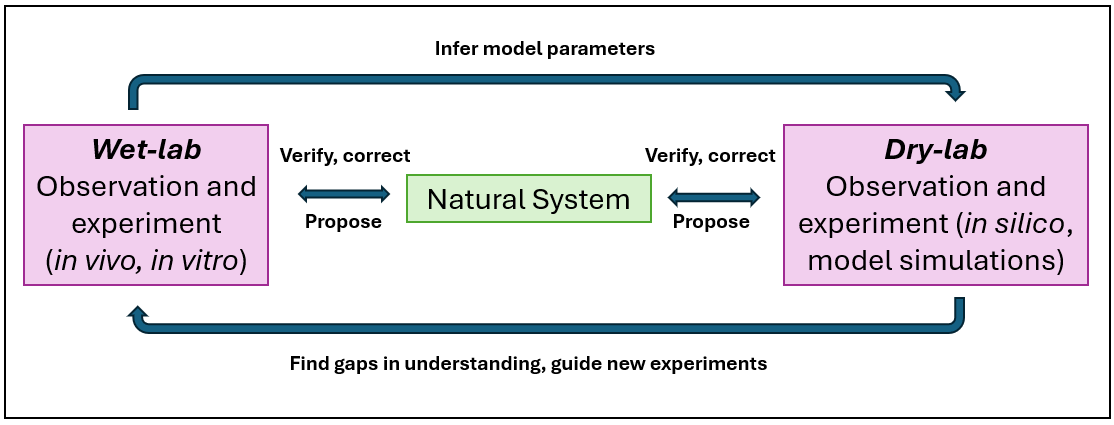
\includegraphics[keepaspectratio]{30-modelling-figures/dry_wet_lab_cycle.PNG}}

}

\caption[Dry and wet lab cycle of
research]{\label{fig-dry-wet-lab-cycle}Computational models can guide
and refine biological experiments and vice versa, creating an iterative
cycle that improves both approaches. Adapted from
{[}\citeproc{ref-szekely2014Stochastic}{251}{]}.}

\end{figure}%

Moreover, using computational methods for studying biological mechanisms
can be time and cost-efficient. Modelling is well positioned for
integration into the experimental cycle of biology. Although \emph{in
vitro} and \emph{in vivo} experiments are still needed to advance our
understanding of biological processes, conducting \emph{in silico}, or
computer-simulated experiments can help guide the wet-lab process by
narrowing the experimental search space
{[}\citeproc{ref-robinson2004Simulation}{253},
\citeproc{ref-reppas2023Leveraging}{254}{]}. Importantly, this creates
an iterative cycle, where computational models inform experimental
design, and experimental findings, in turn, refine and improve the
models. This continuous process strengthens both approaches, leading to
a deeper and more accurate understanding of biological systems
(Figure~\ref{fig-dry-wet-lab-cycle}).

In addition to the reasons discussed, my preference for computational
modelling over wet-lab experiments is also shaped by personal
considerations. Among these personal reasons, is my desire to move away
from animal experimentation, as the speciesist assumption that testing
on animals is both acceptable and necessary does not align with my
values. A detailed and nuanced discussion of this perspective is
provided in Chapter~\ref{sec-data-hazards-chapter}. Following the
principles of the ``3Rs alternatives'' framework: replacement,
reduction, and refinement of animal use in research; I am particularly
committed to the goals of replacement and reduction. I don't believe in
the speciesist beliefs that place one species above another, justifying
the harm of those deemed inferior for research
{[}\citeproc{ref-lafollette1995Utilizing}{255}--\citeproc{ref-jaquet2021Debunking}{257}{]}.

In my opinion, computational modelling research such as the one
undertaken in this PhD, however, cannot be fully separated from animal
research because experimental data is often derived from studies that
have involved using animals to a certain degree
{[}\citeproc{ref-dominguez-oliva2023Importance}{258},
\citeproc{ref-mukherjee2022Role}{259}{]}. Moreover, models must usually
be validated against experimental results to confirm their biological
relevance, and in many cases, such validation still depends on data from
\emph{in vivo} or \emph{in vitro} studies
{[}\citeproc{ref-madden2020Review}{260}{]}. Nevertheless, I advocate for
a shift toward computational research that not only minimizes reliance
on animal studies but also emphasizes reproducibility. Ensuring that
research is reproducible helps avoid redundant experimentation by
allowing scientists to verify and build upon existing findings rather
than repeating studies due to unclear methodologies or irreproducible
results {[}\citeproc{ref-pound2004Where}{261}{]}. When computational
models are rigorously validated and openly shared, they can serve as
reliable references, reducing the need for additional animal-based
experiments to confirm previous findings. Reproducibility and openness
of computational models is further discussed in
Chapter~\ref{sec-open-repro-chapter}.

\section{How do we model biochemical systems
networks?}\label{sec-how-do-we-model}

When constructing a computational model for biochemical system networks,
one of the first steps researchers must undertake is identifying the key
components of the system and the critical interactions between them.
There is no single applicable method for this, as the approaches and
questions will vary depending on the specific study being conducted,
just like in wet-lab experiments. For instance, is it necessary to
represent the behaviour of the system in three dimensions, or would a
two-dimensional approximation be sufficient, or is spatial information
necessary at all? Similarly, should individual cells and molecules be
explicitly modelled, or can their behaviour be adequately captured using
appropriate constitutive equations? Other factors to consider include
determining which interactions between components are essential for the
model and assessing the role of stochastic influences on these
interactions. These examples are not exhaustive, as the questions and
decisions depend on the system studied, the hypotheses being tested, the
study approach, and more. A detailed description of factors chosen for
the model in this project are given in
Chapter~\ref{sec-model-description}. Although each assumption made at
this stage may introduce differences between the model and the
biological system it seeks to emulate, well-considered assumptions
-chosen based on biological knowledge, empirical evidence, and modelling
best practices- can improve the model's clarity, providing a solid
foundation for effective representation of the biological system.

Deciding which simplifications and choices to make during the creation
of a model requires a deep understanding of the system combined with
mathematical and computational skills. Modelling biochemical systems
networks is usually a combined effort between modellers and biologists
(although these roles are not exclusive). This interdisciplinarity is a
key strength of the process, as it means modelling combines diverse
expertise, encouraging a more holistic understanding of diverse
perspectives.

Once the key factors to be modelled have been identified, conceptual
elements of the model can be translated into a mathematical framework.
This process involves defining aspects such as state variables, as well
as representing components of the system using appropriate data types to
model the system. Each interaction within the system may then be
characterised by appropriate mathematical relationships too. For
instance, biochemical reactions can be expressed through differential
equations that describe the rate of change in the concentrations of
reactants and products. The implementation of suitable algorithms to
accurately realise the various components of the model is critical in
ensuring its functionality and efficiency.

For example, is deterministic modelling or stochastic modelling more
suitable for studying a particular system of interest? See deterministic
modelling and stochastic modelling below. Additionally, there is an
expanding array of tools and modelling approaches available that
researchers can choose from
{[}\citeproc{ref-ghosh2011Software}{262}--\citeproc{ref-kohl2011Standards}{265}{]};
translating biological processes into mathematical models on a computer
requires not only the appropriate algorithms but also a suitable
programming language. There is a wide range of programming languages to
choose from ---such as Python, MATLAB, and C to name a few- each with
its own advantages and limitations. In the following sections, we will
explore the modelling approaches and programming languages that are
relevant to this PhD.

\subsection*{Reaction-based modelling:}\label{reaction-based-modelling}
\addcontentsline{toc}{subsection}{Reaction-based modelling:}

When translating biological and chemical systems (such as CaMKII and
NMDARs interactions in the postsynaptic neuron) into algorithms, one way
of describing these systems can be through networks of chemical
reactions {[}\citeproc{ref-cook2009Programmability}{266}{]}. This
approach is known as \emph{reaction-based modelling}, where mathematical
models are used to represent the dynamics of biological systems in a
computer {[}\citeproc{ref-besozzi2016ReactionBased}{267}{]}.
Reaction-based models are formalized as sets of reactions that describe
the given system in terms of mechanistic interactions between the
species of interest. This is, biochemical networks are a set of chemical
species that can be converted into each other through chemical
reactions.

The focus of biochemical network models is usually on the levels of the
chemical species and this usually requires explicit mathematical
expressions for the velocity at which the reactions proceed (kinetic
reaction rates). Once kinetics have been specified, these systems can be
used directly to construct full dynamic simulations of the system
behaviour {[}\citeproc{ref-cook2009Programmability}{266}{]}.

Biochemical network models allow us to gather insight by simulating
chemical interactions over time; we can observe changes in species
levels, visualise stable states within the system, and look for
potential direct or indirect causal relationships between the species
being studied. Importantly, the modellers can modify any of these
parameters to test how such changes impact the model's results.
Computational models allow us to modify parameters in ways that would be
extremely difficult or even impossible to test experimentally, such as
precisely controlling molecular concentrations of molecules in
particular states, eliminating specific interactions, or simulating
conditions that cannot be easily replicated in a laboratory setting.
Using a reaction-based approach is particularly useful for modelling the
interactions of molecules of interest in this PhD, where we can simulate
various chemical components such as NMDARs and CaMKII among others and
their interactions in an efficient manner, as seen in
Chapter~\ref{sec-model-description}.

Biological systems can be simulated in different ways using different
algorithms depending on the assumptions made about the underlying
kinetics {[}{[}\citeproc{ref-resat2009Kinetic}{268}{]};{]}, as discussed
below; and different formalisms are usually applied to describe the
dynamics of these biochemical systems
{[}\citeproc{ref-marchetti2017Simulation}{269}{]}. The kinetics of
chemical reactions vary based on the timing of molecular interactions,
with reactions unfolding over a timescale determined by the microscopic
mechanics involved. Molecular collisions occur randomly inside cells,
and are influenced by factors like thermal motion and diffusion. This
randomness means that the number of molecules of a particular species
fluctuates as a random variable
{[}\citeproc{ref-mazo2008PROBABILITY}{270},
\citeproc{ref-earnest2018Simulating}{271}{]}.

However, when we observe large-scale, or macroscopic, quantities ---such
as the concentration of a substance over time--- the outcomes tend to be
consistent and predictable. This predictable trend enables us to develop
rate laws, mathematical expressions that describe how the concentration
of molecules changes over time. Rate laws are foundational to
deterministic modelling, as they assume that, given a specific starting
point (initial conditions), the progression of a chemical process is
fixed or ``predestined.'' Deterministic models thus allow scientists to
predict the time evolution of chemical concentrations with high
reliability and precision, meaning the predicted trajectory is
consistent and reproducible for a given set of initial conditions, even
though the actual molecular interactions remain random on a microscopic
level. Deterministic models work well where molecular species exists in
vast quantities. However, as systems decrease in scale, such as in the
confined environment of a cell's cytosol, random fluctuations in
molecular populations become significant, making experimental results
less reproducible and measurements more variable. Unlike deterministic
models, which assume smooth, predictable changes, stochastic models
accommodate the random fluctuations in molecule numbers that can
significantly impact reaction outcomes in confined environments. Lets
briefly examine the reasons why each of these approaches may be employed
for distinct purposes:

\subsection*{Deterministic modelling:}\label{deterministic-modelling}
\addcontentsline{toc}{subsection}{Deterministic modelling:}

Deterministic approaches to chemical kinetics are often used to
characterize time evolutions of chemical reactions in large systems
{[}\citeproc{ref-marin2019Kinetics}{272}{]}. A popular representation
for these models is to use ordinary differential equations (ODEs) to
describe the change in the concentrations of chemical species
{[}\citeproc{ref-hoops2016Chapter}{273}{]}. Running the same set of
parameters using deterministic simulations will produce the same results
each time by solving these ODEs. Such descriptions are appropriate when
the number of particles involved in the biochemical network is large
enough to be able to consider continuous concentrations and when spatial
effects are negligible, i.e.~well-mixed environment is assumed and space
has no effect on reactions. In ODE-based models, each chemical species
in the network is represented by an ODE that describes the rate of
change of that species along time. Therefore, ODE models of biochemical
processes are useful and accurate in the high-concentration limit, but
often fail to capture stochastic cellular dynamics accurately because
the deterministic continuous formulation assumes spatial homogeneity and
continuous molecular concentrations
{[}\citeproc{ref-johnson2021Quantifying}{274},
\citeproc{ref-smith2019Spatial}{275}{]}.

These ODE models can be used to simulate the dynamics of the
concentrations of the chemical species along time given their initial
values. This is achieved by numerical integration of the system of ODE
which can be carried out with well-established algorithms
{[}\citeproc{ref-postawa2020Comprehensive}{276}{]}. They are also useful
to find, for example, steady states of the system, which are conditions
when the concentrations of the chemical species do not change
{[}\citeproc{ref-maly2009Introduction}{277}{]}.

\subsection*{Stochastic modelling:}\label{stochastic-modelling}
\addcontentsline{toc}{subsection}{Stochastic modelling:}

As a general rule, stochastic simulations are preferred where the
numbers of particles of a chemical species is small
{[}\citeproc{ref-szekely2014Stochastic}{251},
\citeproc{ref-gillespie2007Stochastic}{278}{]}; the ODE approach is
required when the number of particles is large because the stochastic
approach might be computationally intractable. However, when the
assumption of continuous concentration fails due to small-scale cellular
environment with limited reactant populations ODE representation also
fails. It is here when stochastic simulations are useful. Unlike ODE
models, which assume continuous concentrations, stochastic simulations
track individual reaction events using probability distribution
functions. Stochastic Simulation Algorithms (SSAs)
{[}\citeproc{ref-szekely2014Stochastic}{251},
\citeproc{ref-gillespie2007Stochastic}{278}{]}, determine the timing and
sequence of reactions based on these probabilities.

It is important to stress that one simulation run according to
stochastic approaches is only one realization of a probabilistic
representation, and thus provides limited amount of information on its
own. When running stochastic simulations, it is important that they are
repeated for a sufficient number of times in order to reveal the entire
range of behaviour presented by such a system to estimate a probability
distribution for each chemical species and its dynamic evolution. The
number of required runs depends on the system's complexity and the
degree of variability in its dynamics, with guidelines available in the
literature {[}\citeproc{ref-ritter2011Determining}{279},
\citeproc{ref-byrne2013How}{280}{]} for determining sufficient sampling
(for example based on statistical confidence intervals).

Ultimately, both SSAs and ODEs offer valuable modelling insights, and
the selection of the appropriate method depends on the specific dynamics
and the level of detail required for simulating the biochemical network
under investigation.

As we have seen, computational modelling has its benefits for studying
biological systems. However, the complexity of these systems presents
unique challenges. Biological systems consist of numerous interacting
components and emergent behaviours, requiring careful consideration of
both individual components and their dynamic interactions. The next
section delves deeper into the concept of complexity in biological
systems, examining the challenges of modelling such networks, and how
these challenges are directly linked to the biological questions of this
PhD. I will also discuss the modelling approaches I employ to handle the
complexity of these systems.

\section{Complexity in Systems Biology: Modelling approaches and
challenges}\label{sec-complexity-systems-biology}

This PhD thesis is grounded in \emph{Complexity Science}, which studies
how interactions between components of a system give rise to emergent
behaviors. Examples of application of Complexity Science can be
predator-prey models, epidemiological modelling of pandemics,
protein-protein interaction networks, models of neurons, and more. When
applied to biology, complexity science often falls under the banner of
\emph{Systems Biology}. Systems biology refers to the quantitative
analysis of dynamic interactions between multiple components within a
biological system, with the goal of understanding the system's behaviour
as a whole. Systems biology entails the study of complex biological
systems by combining mathematical modelling, computational simulation,
and biological experimentation.

Complexity is a critical aspect of the systems studied in this project,
that is, the spatiotemporal dynamics of molecules such as CaMKII and
NMDARs in the PSD; making it essential to understand our choices in how
and why we model these elements. Specifically, this project looks at
catalytic interactions that drive post-translational modifications such
as enzyme-driven phosphorylation of CaMKII and NMDARs, as well as
interactions between these proteins that promote the assembly of
molecular complexes {[}\citeproc{ref-sanhueza2013CaMKII}{9},
\citeproc{ref-2015Biochemical}{10}{]}. These types of interactions are
hallmark drivers of something known as \emph{combinatorial complexity}
in cellular systems and biochemical networks
{[}\citeproc{ref-klamt2002Combinatorial}{281}{]}.

When proteins interact, they create unique states that alter the
protein's function, structure, or binding capabilities. Meaning that
each protein can undergo multiple types of modifications or engage in
various site binding interactions, which leads to a multitude of
distinct protein configurations. Systems of interacting proteins are
inherently complex as the interactions between its constituent proteins
usually have the potential to create a vast array of distinct chemical
species. This number can far exceed the actual count of proteins or
protein interactions within the system itself, creating a combinatorial
explosion where every modification or binding event adds another layer
of potential molecular arrangements. This high number in potential
molecular arrangements is referred to as \emph{combinatorial
complexity}, a defining feature of cellular systems and biochemical
networks {[}\citeproc{ref-stefan2014Multistate}{282}{]}.

Moreover, these distinct molecular species states do not exist in
isolation. They are interconnected through an extensive network of
reactions, further amplifying the system's complexity. Intricate network
of protein--protein interactions is in fact a prominent feature of any
signal-transduction system {[}\citeproc{ref-gomperts2009Signal}{283},
\citeproc{ref-hunter2000Signaling}{284}{]}. These interactions can occur
at multiple levels, including feedback loops, cross-talk between
pathways, and spatial-temporal variations. Each reaction acts as a link
within a larger network, creating pathways that connect different
species. Modelling these networks is therefore particularly complex due
to the difficulty in capturing all possible interactions and the
uncertainty in the exact nature of these interactions; i.e.~not all
possible states of a molecular species may be relevant for its functions
{[}\citeproc{ref-pharris2019Multistate}{185},
\citeproc{ref-changeux2005Allosteric}{285}{]}.

The magnitude of combinatorial complexity can be exemplified well with
the CaMKII holoenzyme studied in this PhD. CaMKII is a multi-subunit
protein that can exist in a vast number of possible functional states,
depending on the modifications and interactions at each subunit. Each of
the individual subunits of CaMKII can have multiple possible states,
influenced by factors such as phosphorylation, binding to calmodulin,
and interactions with other proteins like NMDARs, and more
{[}\citeproc{ref-nicoll2023Synapticc}{154}{]}. It has been proposed that
a CaMKII dodecamer could potentially exist in as many as \(10^{20}\)
possible states (see calculations in methods section and appendix S1 in
{[}\citeproc{ref-pharris2019Multistate}{185}{]}). Moreover, the fact
that the potential states of CaMKII vastly outnumber the actual CaMKII
molecules in a dendritic spine
{[}\citeproc{ref-pharris2019Multistate}{185}{]}, suggests that not all
states occur with the same frequency and therefore not all
mathematically calculated states are of equal biological relevance,
which highlights the challenges of modelling systems that involve
combinatorial complexity.

Combinatorial complexity of signalling systems involving multi-state
proteins impacts both the process of writing the model, known as the
\emph{specification problem}, and the computational demands of running
it, particularly in terms of time and resources, known as the
\emph{computation problem}
{[}\citeproc{ref-stefan2014Multistate}{282}{]}. The specification
problem encompasses challenges such as representing all possible states
of a molecule like CaMKII, the various complexes it can form, the
transformations those complexes can undergo, and the parameters and
conditions that govern these processes, all in a robust and efficient
manner. When faced with the computation problem, where it may become
computationally infeasible to enumerate or simulate all state and
network possibilities, the model may become intractable, requiring
excessive time and resources to compute, store and/or analyse.

As explored next, rule based modelling provides a powerful solution to
the specification problem: rather than accounting for every possible
state explicitly, it enables a focus on biologically significant states
while allowing emergent behaviours to arise through rule-based
interactions. As for the computation problem, we will see later on how
particle-based rule evaluations can help with it.

\section{Rule based modelling}\label{rule-based-modelling}

The challenges posed by the specification problem of combinatorial
complexity motivate the adoption of a rule based modelling (RBM)
approach for simulating cell signalling systems in this PhD. RBM can
help by using a set of logical rules to describe how molecules interact
with each other. With this type of modelling, the system is modelled by
specifying the reactions (or rules) that describe how molecules interact
and change
{[}\citeproc{ref-harris2009Compartmental}{286}--\citeproc{ref-chylek2015Modeling}{288}{]}.
Instead of listing every individual interaction or molecular species
explicitly, rules are used to represent how molecules bind, modify, and
transform. These rules, which are primarily based on experimental
observations, are applied to sets of molecules that can be in different
states or configurations, and the overall dynamics of the system emerge
from the repeated application of these rules. This method allows for
more efficient specification of models, and can scale to handle complex
systems like the ones studied in this PhD; this way, avoiding the
impossible enumeration of the \(10^{20}\) calculated states of CaMKII
alone.

\subsection*{BioNetGen: A tool for rule based
modelling}\label{bionetgen-a-tool-for-rule-based-modelling}
\addcontentsline{toc}{subsection}{BioNetGen: A tool for rule based
modelling}

BioNetGen (Biological Network Generator)
{[}\citeproc{ref-harris2016BioNetGena}{245}{]} is a useful tool for
performing RBM of biochemical networks, particularly in the context of
signalling systems and protein--protein interactions. BioNetGen uses a
language called BNGL (BioNetGen Language) to define molecular species
and the rules that govern their interactions. A key feature of BNGL is
that it allows researchers to describe the interactions between proteins
and other molecules in a high-level, abstract form, without the need to
manually enumerate every possible molecular species or state. Instead,
BNGL allows users to define generalized rules using an RBM approach,
specifying how molecular entities can interact -such as binding,
phosphorylation, or degradation --- along with the conditions under
which these interactions occur.

Different approaches to RBM are used depending on one's objectives and
modelling focus
{[}\citeproc{ref-schaff2016Rulebased}{289}--\citeproc{ref-boutillier2018Kappa}{292}{]}.
In our approach, we employ BioNetGen and its associated language BNGL,
as it provides some key advantages for the research at hand. Firstly,
BNGL provides a language that is tailored towards modelling biochemical
networks with domain-specific requirements, allowing for the detailed
specification of molecules and their binding domains, which is
particularly useful for studying protein post-translational
modifications, for example autophosphorylation of CaMKII. Moreover, BNGL
helps resolve nomenclature challenges by allowing explicit naming of
molecules, binding sites, and modification states in a structured and
consistent manner (see Figure~\ref{fig-camkii-dodecamer} for an in depth
example of CaMKII nomenclature using BNGL). The ability to model
site-specific details of protein-protein interactions allows these
dynamics to be captured systematically.

Guided by the ``don't care, don't write'' principle at the heart of RBM
modeling {[}\citeproc{ref-chylek2014Rulebased}{287}{]}, BNGL allows us
to specify only the relevant states for a given reaction. This approach
eliminates the need to define every possible state explicitly. That is,
the rules determine when an implicitly defined reaction can happen and
then, for any given iteration, only the states that matter for the
execution of a particular reaction (or rule) are explicitly declared.
States that do not matter to a particular rule can be omitted. For
instance, lets consider a reaction rule where a CaMKII subunit binds to
a CaM molecule (Figure~\ref{fig-bngl-rbm-example}).

\begin{figure}

\centering{

\pandocbounded{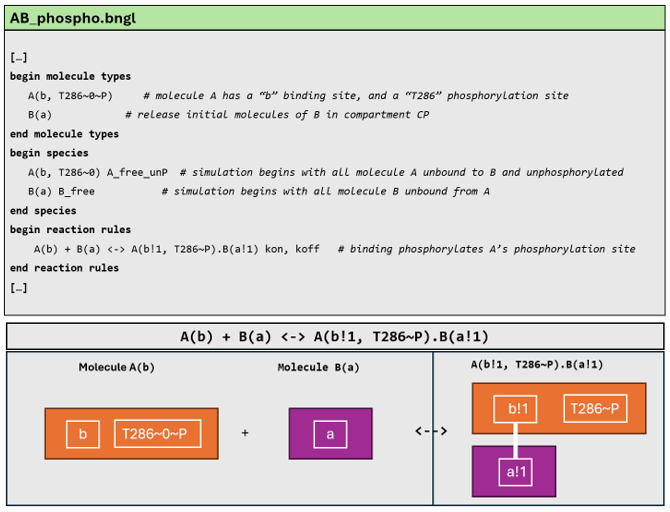
\includegraphics[keepaspectratio]{30-modelling-figures/AB_phospho.PNG}}

}

\caption[BioNetGen Language rule based modelling
example]{\label{fig-bngl-rbm-example}A and B molecule binding causes
phosphorylation; an example of don't care, don't write in BNGL. The
possible states of molecules A and B are defined under the molecule
types block. Molecule A has a binding site (b) and a phosphorylation
site (T286), which can exist in a phosphorylated (\textasciitilde P) or
unphosphorylated (\textasciitilde0) state. Molecule B is defined simply
with a single binding site (a). The initial states of these molecules
are defined in the species block, which specifies how the molecules are
introduced at the start of the simulation. Molecule A is released with
its binding site (b) free (unbound to B) and its phosphorylation site in
the unphosphorylated state (T286\textasciitilde0). Molecule B is
released in a free state, unbound to molecule A. The reaction rules
block defines how the molecules interact. In this example, the rule
specifies that phosphorylation occurs when molecules A and B bind
(indicated by the ``!1'' link notation). Importantly, the state of A's
phosphorylation site does not need to be explicitly stated in the rule.
What is required for the reaction to occur is the binding of A and B,
after which phosphorylation can take place. While this is a simple
example with limited complexity, as more possible states are introduced,
the value of this method becomes clearer. Note this example does not
represent a complete BNGL model, as indicated by the ``{[}\ldots{]}'',
which denote additional model definitions that would typically appear
before and after these lines.}

\end{figure}%

In the example shown in Figure~\ref{fig-bngl-rbm-example}, we don't
specify the state of T286 in the reaction rule of A and B leading to
phosphorylation of the former. Instead, we only specify the states that
are relevant for a specified reaction (in this case, that molecule A has
a free binding site to bind with B, and vice versa) and the rest is left
unspecified. In more complex models such as the one used in this thesis,
this dramatically reduces the number of reactions that need to be
written
{[}\citeproc{ref-karp1975Computational}{293}--\citeproc{ref-suarez2009Challenges}{296}{]}.
Details of how this is done in our model are described in
Chapter~\ref{sec-model-description}.

Additionally, BNGL supports the inclusion of cellular compartments
through its compartmental extension (cBNGL), enabling explicit modelling
of the compartmental organization of the cell and its effects on system
dynamics {[}\citeproc{ref-harris2009Compartmental}{286}{]}. This way, we
can introduce localization attributes for molecular species, as well as
appropriate volumetric scaling of reaction rates. BioNetGen and its
associated language BNGL have been integrated with MCell via pyBNGL, a
Python library {[}\citeproc{ref-husar2022MCell4}{244}{]}. As we will see
next, this provides further advantages when it comes to the computation
problem of combinatorial complexity.

\subsection*{MCell: A tool for dynamic protein visualisation and
modelling}\label{mcell-a-tool-for-dynamic-protein-visualisation-and-modelling}
\addcontentsline{toc}{subsection}{MCell: A tool for dynamic protein
visualisation and modelling}

MCell (Monte Carlo Cell) is an agent-based (also known as
particle-based) reaction-diffusion software platform designed to
simulate complex biochemical processes with a focus on spatial and
stochastic dynamics
{[}\citeproc{ref-stiles1996Miniaturea}{241}--\citeproc{ref-husar2022MCell4}{244}{]}.
Agent-based modelling simulates the interactions of autonomous agents
-such as molecules- to understand how a system behaves and to capture
emergent behaviours; for example, the formation of molecular complexes,
signal transduction pathways, or spatial patterning within a cell. MCell
is particularly valuable for modelling biological systems where the
precise location and movement of molecules are crucial, such as synaptic
signalling or interactions at the cellular level studied in this PhD. To
facilitate the visualisation of these complex geometries, MCell
integrates with CellBlender. CellBlender is an addon for Blender, a
widely used open-source 3D modelling and animation software
{[}\citeproc{ref-gupta2018Spatial}{297}{]}.

Reaction-based models typically rely on networks to represent chemical
interactions (as discussed in
Section~\ref{sec-complexity-systems-biology}), but they can become
computationally expensive as system complexity grows, especially when
handling large numbers of reactions or species. MCell, however, bypasses
this limitation by tracking individual molecules and their interactions
in real-time, only focusing on the relevant species and states. Its
particle-based rule evaluation eliminates the need to construct full or
partial reaction networks, both at the start and during the simulation,
by concentrating solely on the molecules present, their current states,
and the reactions they can participate in at any given moment. This
approach, known as network-free simulation, not only reduces
computational demands but also allows researchers to explore more
complex and realistic biological scenarios without the constraints of
predefined reaction networks.

As a spatial particle-based simulator, MCell models molecules as point
particles within a 3D space. Each time step of an MCell simulation,
particles can move, interact with other particles or surfaces, and
undergo bimolecular and/or unimolecular reactions. Briefly, MCell
operates as follows: as a volume molecule diffuses, all molecules within
a given radius along its trajectory, or at the point of collision on a
surface, are considered for a reaction. For surface molecules (in
membranes), the molecule first diffuses, and then its neighbours are
evaluated for reaction Figure~\ref{fig-mcell-works}. Moreover, MCell
allows defining arbitrary geometry, and complex models such as a 180
\(\mu\text{m}^3\) 3DEM reconstruction of hippocampal neuropil have been
used to construct a geometrically-precise simulation of 100s of neuronal
synapses at once {[}\citeproc{ref-bartol2015Computational}{298}{]}. A
detailed description of mathematical foundations of MCell's algorithms
can be found here {[}\citeproc{ref-kerr2008FAST}{243},
\citeproc{ref-bartol2000Monte}{299}{]}

\begin{figure}

\centering{

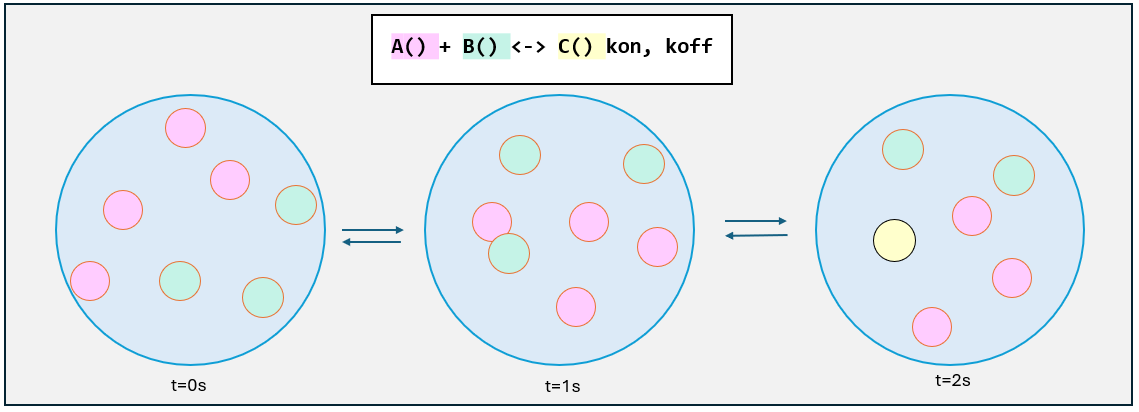
\includegraphics[width=0.85\linewidth,height=\textheight,keepaspectratio]{30-modelling-figures/mcell_works.PNG}

}

\caption[MCell simplified schematic to understand how particle collision
works]{\label{fig-mcell-works}MCell simplified schematic to understand
how particle collision works. At time zero, molecules are released into
a 3D space (represented by a blue circle), and they begin to diffuse
according to specified diffusion coefficients (not shown). Over time, if
molecules A and B collide, they are considered for a reaction, in this
case, where A and B combine to form molecule C, with kinetic rates kon
and koff.}

\end{figure}%

MCell software employs stochastic Monte Carlo algorithms, which rely on
random sampling to simulate the behaviour of molecules. This stochastic
approach makes MCell particularly effective for capturing the inherent
randomness found in biological systems, previously discussed in
Section~\ref{sec-how-do-we-model}. MCell can model the diffusion of
molecules within cellular compartments and the probabilistic
interactions between proteins, making it a powerful tool for studying
phenomena where small fluctuations can have significant impacts, such as
in the postsynaptic signalling pathways studied in this thesis.

MCell4 (version 4, the one used here) also provides a versatile Python
interface. This recently implemented Python interface allows for greater
ease in scripting and model construction, making it more user-friendly
and adaptable for researchers {[}\citeproc{ref-husar2022MCell4}{244}{]}.
Additionally, the newly created BioNetGen Library for python (pyBNG)
allows direct loading and parsing of a BNG model into MCell. This allows
for the creation of models that capture multimeric structures,
site-specific binding properties, and the dynamic interactions of
proteins over time and space {[}\citeproc{ref-husar2022MCell4}{244}{]}.
Next, we provide a more detailed discussion emphasizing how this
approach supports the goals of this PhD project.

\subsubsection*{MCell and BioNetGen
integration}\label{mcell-and-bionetgen-integration}
\addcontentsline{toc}{subsubsection}{MCell and BioNetGen integration}

The main components of MCell4 (henceforth MCell), which enable
interaction between various libraries and engines, include: a PyMCell
library which offers a Python interface and contains classes to manage
the model representation. The MCell4 engine, responsible for executing
simulation algorithms, and a pyBNG library, which provides methods for
resolving BioNetGen reactions Figure~\ref{fig-mcellparsing}.

\begin{figure}

\centering{

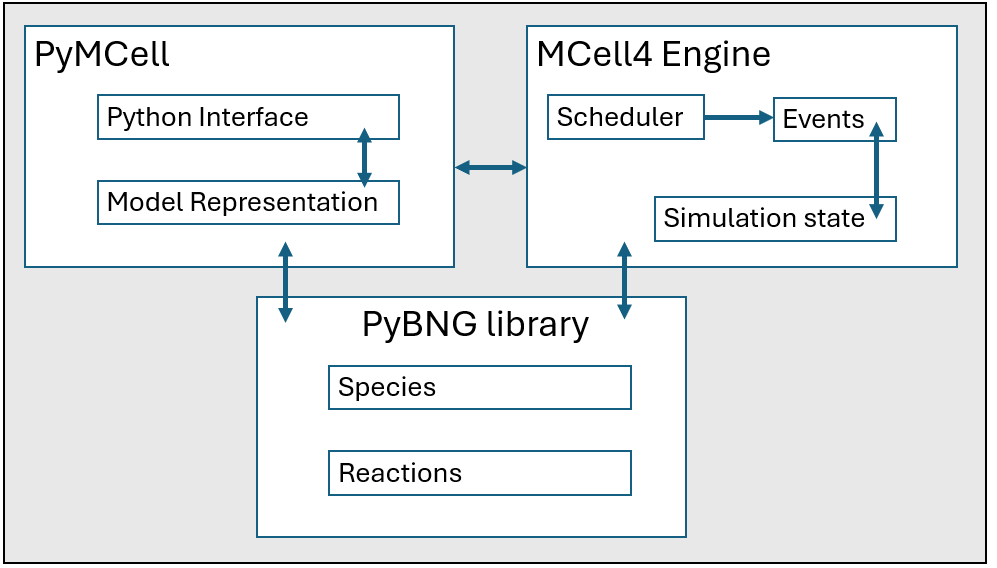
\includegraphics[width=0.7\linewidth,height=\textheight,keepaspectratio]{30-modelling-figures/mcellparsing.PNG}

}

\caption[MCell components]{\label{fig-mcellparsing}The MCell4 (version
used in this PhD) components that allow for integration between
different libraries and engines. PyMCell Library allows for python
interface for model representation. The MCell4 engine implements
simulation algorithms through a scheduler that keeps track of events to
be run in each iteration. The pyBNG library provides methods to resolve
BioNetGen reactions using python scripts. Figure modified from
{[}\citeproc{ref-husar2022MCell4}{244}{]}.}

\end{figure}%

A model can be defined using BNGL, where molecular interactions are
specified through detailed rules and reactions. This model can then be
parsed using the pyBNG library, allowing Python scripts to handle the
BNGL files and initiate simulations with MCell. Python scripts play a
crucial role in this workflow. They are not only responsible for parsing
BNGL files but also for defining the cellular geometry and setting
parameters required for MCell simulations. Once the simulation is
executed in MCell, the output is generated in the form of data files,
containing time-series data on molecular concentrations and dynamics as
dictated by the initial reactions (see Figure~\ref{fig-input-output}).

To illustrate the integration between MCell and BioNetGen using python
scripts, see Figure~\ref{fig-bngl-workflow}, where a BNGL file defines
species, reaction rules, molecule released and compartments. These
elements are then imported into MCell, as shown in
Figure~\ref{fig-mcell-workflow}, through a python script that ``calls''
the BNGL file to run it through MCell, using the mechanisms described in
Figure~\ref{fig-mcellparsing}.

Standard BNGL files, such as the one shown in
Figure~\ref{fig-bngl-workflow}, are compatible with tools like BioNetGen
itself, which enables rapid validation of a reaction network using
BioNetGen's ODE or SSA solver or other analysis tools
{[}\citeproc{ref-harris2016BioNetGena}{245}{]}. This method allows the
model to be directly compared with spatial simulation results in MCell4,
eliminating the need of creating multiple versions of the same model.
This integration of tools not only provides a more accurate depiction of
cellular dynamics but also enhances reproducibility, as the Python
scripting enables the simulations to be replicated and adjusted easily.
While this overview provides a general understanding of the model's
inputs and outputs, specific methodological details will be elaborated
in Chapter~\ref{sec-model-description}.

For a simpler but more comprehensive model that incorporates detailed
compartments and cell geometry, you can access, download and execute the
code here \href{https://github.com/Susana465/test_ABC}{TEST\_ABC}. This
repository includes a set of models where spatial features are taken
into consideration, and a thorough README is provided with step-by-step
instructions that are beyond the scope of this introduction chapter.

Altogether, the integration of MCell and BioNetGen provides a robust
framework for addressing key challenges in this PhD project. BioNetGen's
rule-based modelling approach effectively addresses the specification
problem arising from the combinatorial complexity of the biochemical
systems under study. By enabling the concise representation of CaMKII as
a multimeric molecule and its interactions with other multimeric
proteins, BioNetGen simplifies the modelling process. MCell complements
this by allowing these molecular interactions to be modelled within
spatially defined geometries. Additionally, the data output from
simulations can be further analysed and interpreted to explore key
behavioural patterns, quantify interaction dynamics, and assess model
accuracy, providing a deeper understanding of the system's behaviour.
The particle-based, network-free simulation capabilities of MCell are
critically helpful for addressing the computational challenges
associated with the combinatorial complexity of CaMKII. Moreover, MCell
enables the stochastic modelling of molecules within defined
environments, such as dendritic spines, providing advantages that are
key for studying the stochastic dynamics relevant to this research.

\begin{figure}[H]

\begin{minipage}{\linewidth}

\centering{

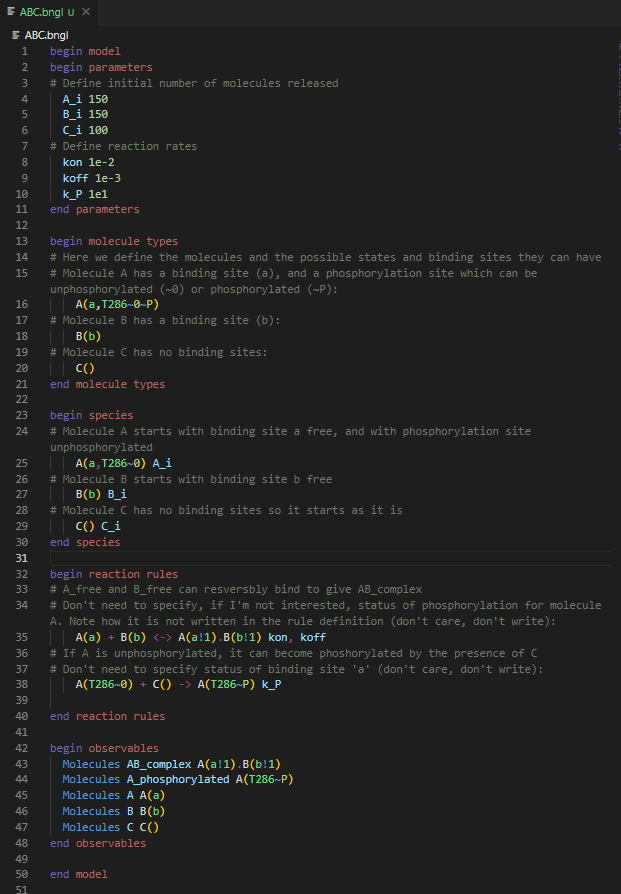
\includegraphics[width=0.7\linewidth,height=\textheight,keepaspectratio]{30-modelling-figures/mcell4BNGLworkflow.PNG}

}

\subcaption{\label{fig-bngl-workflow}An example BNGL model file titled
``ABC.bngl'' includes initial parameters, defined compartments, and
species within those compartments. It also contains a simple reaction
rule, where A + B produces C, and the reverse reaction is also
possible.}

\end{minipage}%
\newline
\begin{minipage}{\linewidth}

\centering{

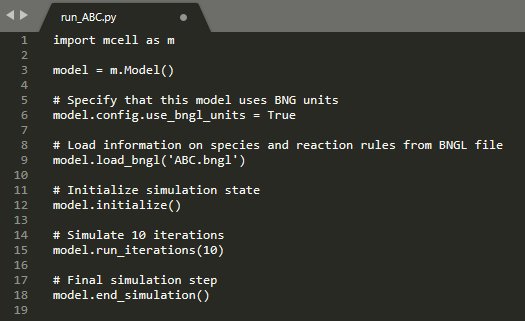
\includegraphics[width=0.7\linewidth,height=\textheight,keepaspectratio]{30-modelling-figures/mcell4BNGLworkflow2.PNG}

}

\subcaption{\label{fig-mcell-workflow}The Python file run\_model.py
imports mcell as a module via the PyMCell library. This script loads the
BNGL file shown in (a), where the entire BNGL file is read, the model is
initialised and run for 10 iterations. Specific parts of the BNGL file,
such as reaction rules or compartment and molecule release information,
can be loaded. BNGL compartments can be replaced with actual 3D
geometry.}

\end{minipage}%

\caption{\label{fig-workflow}BNGL and PyMCell workflow.}

\end{figure}%

\subsubsection*{Birds eye view of model inputs and
outputs}\label{birds-eye-view-of-model-inputs-and-outputs}
\addcontentsline{toc}{subsubsection}{Birds eye view of model inputs and
outputs}

To provide an overview of the implementation of model files
(Figure~\ref{fig-workflow}) and to clarify the overall process of what
goes into a model and what is generated, see a simplified illustration
in (Figure~\ref{fig-input-output}). The inputs to the model are the
model files, which are written in the chosen modelling language, such as
Python or BioNetGen. These input files include the reaction rules, the
definitions of molecular species, and other parameters that define the
model. The molecular interactions defined in these models are executed
and simulated within a 3D environment, and an output is produced,
typically displaying changes in molecular concentrations over time.

In the context of this PhD, this involves constructing a model that
defines CaMKII and NMDAR interactions, along with other relevant
molecules (detailed in Chapter~\ref{sec-model-description}). These
interactions are simulated within a postsynaptic dendritic volume, and
the resulting data captures the variations in molecular concentrations
over time. Capturing the variations in molecular concentrations over
time allows for a detailed analysis of the kinetics of these
interactions, providing insights into the rates and mechanisms of
biochemical reactions at a level of precision that is challenging to
achieve experimentally. This information can then reveal how specific
molecular dynamics contribute to larger-scale cellular behaviours like
LTP for understanding how learning and memory work. Additionally,
understanding the chemical properties of the reactions involved,
including binding affinities, reaction rates, and diffusion
characteristics, can aid in predicting how changes at the molecular
level may impact the overall function of the synapse.

\begin{figure}

\begin{minipage}{\linewidth}

\centering{

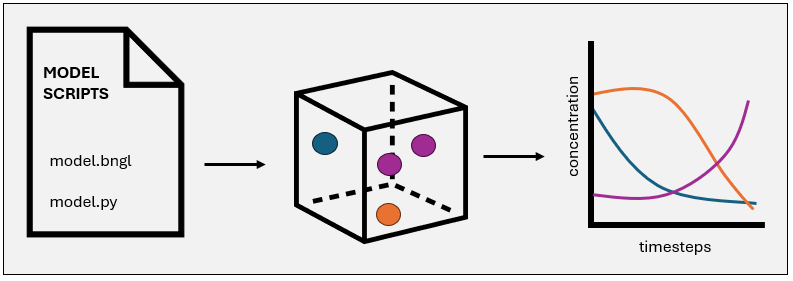
\includegraphics[width=0.9\linewidth,height=\textheight,keepaspectratio]{30-modelling-figures/inputoutput.PNG}

}

\subcaption{\label{fig-input-output}What goes in and what comes out when
modelling. An overview of input and output workflow of models in this
project. Input files define the model, which is run to simulate
diffusion of molecules in a 3D space, to give an output of molecular
concentrations across time.}

\end{minipage}%
\newline
\begin{minipage}{\linewidth}

\centering{

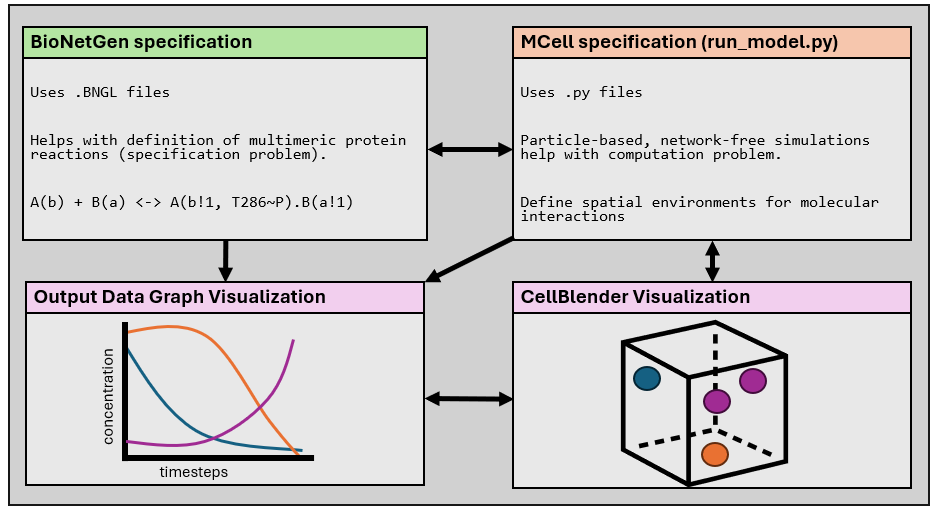
\includegraphics[width=0.9\linewidth,height=\textheight,keepaspectratio]{30-modelling-figures/inputoutput2.PNG}

}

\subcaption{\label{fig-input-output2}There are alternative workflows for
modelling and visualisation. BioNetGen uses .BNGL files to define
biochemical reactions. MCell uses .py files. Outputs from either path
can be visualised as graphs of molecular concentration over time or as
3D spatial distributions in CellBlender. The arrows emphasise the
flexible flow between tools, showing how BioNetGen and MCell outputs can
be independently or jointly visualised to provide both temporal and
spatial insights into molecular dynamics.}

\end{minipage}%

\caption{\label{fig-workflow}Modelling workflow.}

\end{figure}%

Not only can BioNetGen and MCell be integrated and used together via the
Python API, but the models created here can, in theory, be further
integrated with software that supports Systems Biology Markup Language
(SBML), a widely recognised standard for representing biological models.
SBML enables the translation and integration of models written in
different formats, allowing them to be executed across a range of
software platforms {[}\citeproc{ref-hucka2003Systems}{300},
\citeproc{ref-keating2020SBML}{301}{]}. As a well-established standard,
SBML is frequently used to describe chemical reaction networks, such as
those involved in metabolic processes or cell signalling pathways.
Critically, BioNetGen can export models written in BNGL to the SBML
format. This export capability allows for the conversion of rule-based
BNGL models into a format that is compatible with SBML-supporting tools,
increasing the flexibility of what future researchers can do with models
like this one.

The ability to export BioNetGen models to SBML not only enhances
interoperability but also aligns with key principles of reproducible and
open science. This is particularly relevant to the FAIR (Findable,
Accessible, Interoperable, and Reusable) principles for research, which
are central to fostering transparency and collaboration in computational
biology. The following chapter builds on these concepts, discussing how
this project embeds openness, reproducibility, and responsible research
practices.

\bookmarksetup{startatroot}

\chapter{Open, Reproducible and Ethics-focused
PhD}\label{sec-open-repro-chapter}

In recent decades, scientific research has accelerated significantly,
with a ``publish or perish'' culture becoming deeply ingrained in the
academic community's consciousness
{[}\citeproc{ref-angell1986Publish}{302},
\citeproc{ref-rawat2014Publish}{303}{]}. Frequent publication is widely
regarded as a powerful tool for scholars to showcase their expertise and
gain recognition among their peers. Likewise, there is a generalised
view that this keeps academics constantly engaged with relevant
knowledge works in their fields of expertise. In theory, it also serves
to benefit the wider public by making scholarly insights available.
Successfully published research not only enhances an individual's
reputation but also raises the profile of their institution, often
attracting greater funding opportunities. Moreover, academic
institutions and universities commonly use the number of publications
credited to a researcher as a key indicator of their competence and
career progression
{[}\citeproc{ref-york2015Defining}{304}--\citeproc{ref-elbanna2023Publish}{306}{]}.
In this view, a strong publication record can be beneficial, opening up
opportunities for researchers and their institutions.

However, this mindset exerts significant pressure on researchers to
continuously publish in order to secure funding and advance their
careers {[}\citeproc{ref-miller2011Publish}{307},
\citeproc{ref-hangel2017Why}{308}{]}. Alongside this, there are
persistent biases in academic publishing, where work affiliated with
prestigious institutions is often (wrongly) perceived as higher quality
than that from less well-known or under-resourced institutions,
regardless of the actual merit of the research
{[}\citeproc{ref-morley2007Employers}{309}--\citeproc{ref-campbell2019Prestige}{311}{]}.
On top of this, the Eurocentric bias where academic knowledge produced
in wealthier countries is often regarded as superior, marginalises and
even dismisses the realities and contributions of the Global South
{[}\citeproc{ref-jazeel2010Limits}{312}--\citeproc{ref-amutuhaire2022Reality}{315}{]}.
Similarly, the expectation for a high volume of publications impacts
disproportionately low-paid academics in resource-constrained countries,
who can face a variety of structural barriers, including limited grant
funding {[}\citeproc{ref-castrotorres2022North}{314}{]} and inaccessible
academic journal costs {[}\citeproc{ref-chan2014Increasing}{316},
\citeproc{ref-collyer2018Global}{317}{]} among many other reasons
{[}\citeproc{ref-hopkins2013Disparities}{318},
\citeproc{ref-willis2021Gender}{319}{]}.

In the culture of continuously publishing and publishing fast, those who
are already at a disadvantage due to systemic bias and oppression are
the ones who continue to lose the most. For example, research has shown
that minoritised communities ---whether this be due to race, gender,
sexual orientation, or other factors--- are underrepresented in
prestigious journals, partly due to implicit biases and the dominance of
Western academic frameworks
{[}\citeproc{ref-hopkins2013Disparities}{318}--\citeproc{ref-boda2022What}{320}{]}.
Consequently, the ``publish or perish'' culture overwhelmingly benefits
scholars in wealthier countries while deepening global inequalities in
knowledge production.

Moreover, a pressure to publish in high impact journals is closely tied
to what is known as publication bias. In published academic research,
publication bias occurs when the outcome of an experiment or research
study biases the decision to publish or otherwise distribute it. This
typically results in a preference for publishing significant or positive
results, disrupting the balance of findings and favouring those that are
deemed novel or noteworthy. Whilst negative or inconclusive results are
rarely published or considered less worthy of publication
{[}\citeproc{ref-thornton2000Publication}{321},
\citeproc{ref-page2021Investigating}{322}{]}.

Examining this bias towards positive results reveals substantial
evidence of a troubling trend: an overrepresentation of false-positive
findings in the scientific literature
{[}\citeproc{ref-sinha2006Reporting}{323}--\citeproc{ref-schneck2023Are}{327}{]}.
This bias towards positive results has several concerning and wasteful
consequences, including, but not restricted to a significant number of
valid negative results remaining unpublished, which excludes critical
findings from the scientific record. This means that other research
teams, unaware of these unpublished negative results, may continue to
unknowingly test the same hypotheses (which may actually be false)
until, by chance or artifact, a positive result is obtained. These
chance positive results are then published, as they align with the
preference for significant findings, even when substantial and more
definitive contradictory evidence may exist in contrast to it
{[}\citeproc{ref-carlson2012Understanding}{328}{]}. What is more, this
underreporting of negative results introduces bias into meta-analysis,
which consequently misinforms researchers, doctors, policymakers and the
public in general {[}\citeproc{ref-afonso2024Perils}{329}{]}.
Additionally, more resources are wasted on already disputed research
that remains unpublished and therefore unavailable to the scientific
community
{[}\citeproc{ref-kicinski2013Publication}{330}--\citeproc{ref-page2019Assessing}{333}{]}.

This cycle sustains an error-prone body of scientific literature,
undermining the reliability of published research. Hand in hand with
this publication bias, comes something now known as a
\emph{Reproducibility Crisis}, where it is becoming increasingly
apparent that making ``fast-science'', while not the sole cause, is
associated with a lack of being able to reproduce research
{[}\citeproc{ref-stengers2016Another}{334},
\citeproc{ref-leite2021Juggling}{335}{]}. The reproducibility crisis has
been on the rise for the past few decades as we uncover the fact that
much of the research that is published fails to be reproduced by others.
To give some examples, a survey of 1576 scientists published in Nature
{[}\citeproc{ref-baker2016500ScientistsLift}{336}{]} reported that over
70\% of the participants failed to reproduce others' experiments and
over 50\% failed to reproduce their own results. Similarly,
{[}\citeproc{ref-tiwari2021ReproducibilitySystemsBiology}{337}{]}
assessed the reproducibility of 455 mathematical models in systems
biology and found that about 50\% of published models were not
reproducible either due to incorrect or missing information in the
manuscript. Importantly, the remaining models could be reproduced,
sometimes with additional effort, highlighting that while
reproducibility is not universal, a substantial fraction of models can
still provide reliable insights when properly documented.

Much of the criticism surrounding the reproducibility crisis centres on
statistical methods and research practices
{[}\citeproc{ref-ioannidis2005Whya}{338}--\citeproc{ref-stefan2023Big}{340}{]}.
Problematic scientific behaviours, such as HARKing (Hypothesising After
the Results are Known), p-hacking (manipulating data analysis to achieve
statistical significance), and selectively reporting only positive
outcomes, as discussed above, have been identified as major contributors
to irreproducibility
{[}\citeproc{ref-wagenmakers2007Practical}{341}--\citeproc{ref-lew2020Reckless}{343}{]}.
Indeed, this reliance on p-values, provided they meet the conventional
threshold of statistical significance (typically p \textless{} 0.05),
can sometimes lead to studies being treated as definitive evidence, even
when their findings are not robust or reproducible
{[}\citeproc{ref-lew2020Reckless}{343}{]}.

The list of factors contributing to irreproducibility is extensive and
is not restricted to statistical methods. A lack of access to raw data
or, in some cases, outright data fabrication also plays a role
{[}\citeproc{ref-flier2017Irreproducibility}{344},
\citeproc{ref-bausell2021Problem}{345}{]}. Ambiguities in experimental
procedures and data analysis steps further undermine research
reliability. On a broader, more systemic level, there's an important
discussion regarding how current academic systems often prioritize
novelty and statistically significant findings, as research funding is
more likely to be secured and promoted when the outcomes are more
profitable
{[}\citeproc{ref-bhandari2004Association}{346}--\citeproc{ref-ebadi2016How}{348}{]}.
Although these behaviours fall under scientific misconduct
{[}\citeproc{ref-science2023Reproducibility}{349}{]} and are not
considered acceptable scientific practice, they continue to occur as the
mindset of publish or perish continues to embed itself in how scientists
work.

Interestingly, a large-scale survey of nearly 6,000 academic
psychologists (with 2,155 responses) assessed self-reported engagement
in some of these questionable research practices (for example
ambiguities in experimental procedures, p-harking, etc) known to
introduce bias into research findings
{[}\citeproc{ref-john2012Measuring}{350}{]}. Notably, respondents often
justified their own use of these practices while simultaneously viewing
them as unacceptable when used by others. This is just one example, and
it is worth noting that scientific standards and methodologies
continuously evolve, meaning that questionable research practices are
not static. Methods once tolerated, or even considered standard, may now
be recognised as problematic, reflecting our ability to reassess and
refine ethical and methodological frameworks. Encouragingly, awareness
of the reproducibility crisis is growing, and there is a gradual shift
towards promoting open and reproducible research practices
{[}\citeproc{ref-nature2018Challenges}{352}{]}.

Together, the issues outlined above, from the reproducibility crisis and
publication bias to the prevalence of questionable research practices,
reveal not isolated failings, but a systemic entanglement that
compromises the integrity, efficiency, and ethical foundation of
scientific research. In this context, the need for a fundamental shift
becomes clear: one that centres reproducibility and accessibility not as
optional enhancements, but as essential to producing ethical and
meaningful research.

While I cannot solve these systemic issues alone, this PhD is an
opportunity to actively engage with them. I am approaching my research
with a conscious commitment to reproducibility, transparency, and
accessibility, while also taking seriously the ethical responsibilities
that come with producing and sharing knowledge. By embedding these
values into the way I design, conduct, and communicate my work, I hope
to contribute to a broader shift towards more inclusive, accountable,
and responsible research practices.

\section{Reproducibility Definition Used in this
PhD}\label{reproducibility-definition-used-in-this-phd}

There is a long history of the terms reproducibility and replicability
being used interchangeably, or their meanings being swapped depending on
the field of study
{[}\citeproc{ref-ivie2018ReproducibilityScientificComputing}{90},
\citeproc{ref-claerbout1992ElectronicDocumentsGive}{353},
\citeproc{ref-plesser2018ReproducibilityVsReplicability}{354}{]}. For
example, a review on the usage of reproducible/replicable meanings
{[}\citeproc{ref-barba2018TerminologiesReproducibleResearch}{355}{]}
showed that most papers and disciplines use the terminology as defined
by Claerbout and Karrenbach
{[}\citeproc{ref-claerbout1992ElectronicDocumentsGive}{353}{]}, whereas
microbiology, immunology and computer science tend to follow the
Association for Computing Machinery use of reproducibility and
replication given by
{[}\citeproc{ref-ivie2018ReproducibilityScientificComputing}{90}{]}. In
political science and economics literature, both terms are used
interchangeably.

In this PhD, we use the definition used by
{[}\citeproc{ref-turingwaycommunity2019TuringWayHandbook}{356}{]}, where
reproducible research is understood as ``\emph{work that can be
independently recreated from the same data and the same code that the
original team used}''. Reproducible, replicable, robust and
generalisable have different meanings as described in the table below.

\begin{figure}

\centering{

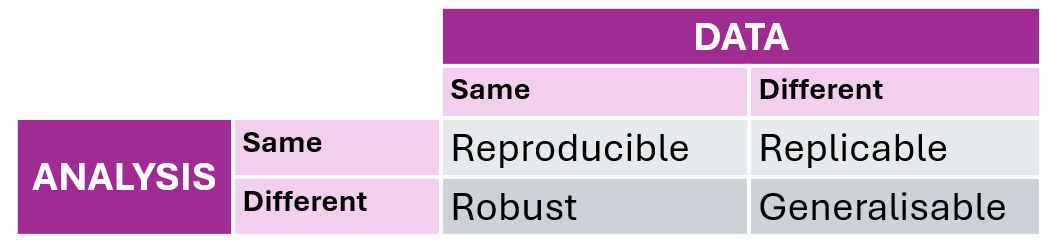
\includegraphics[width=0.65\linewidth,height=\textheight,keepaspectratio]{22-reproducibility-figures/repro_definintions.PNG}

}

\caption[How The Turing Way defines reproducible
research]{\label{fig-repro-definitions}How The Turing Way defines
reproducible research. Adapted from
{[}\citeproc{ref-turingwaycommunity2019TuringWayHandbook}{356}{]}.}

\end{figure}%

\begin{itemize}
\item
  \textbf{Reproducible research}: is obtained when same analysis is
  performed on the same data, to produce the same results.
\item
  \textbf{Replicable research}: refers to conducting the same analysis
  on different datasets, resulting in qualitatively similar outcomes.
\item
  \textbf{Robust research}: entails subjecting the same dataset to
  different analysis workflows to address the same research question,
  such as employing distinct pipelines in R and Python. Robustness
  demonstrates that findings can remain consistent regardless of
  different methods used for analysis, indicating validity and
  resilience to various factors like changes in conditions or methods
  (such as different programming languages).
\item
  \textbf{Generalisable research}: refers to findings or conclusions
  that can be applied beyond the specific context in which they were
  derived. It indicates that the results are not limited to a particular
  dataset, methodology, or experimental setup, but instead can be
  extended to broader populations, situations, or conditions. By
  combining replicable and robust research, we can obtain more
  generalisable results.
\end{itemize}

\section{Open Science}\label{open-science}

Open Science is an approach to the scientific process that promotes
cooperative work and new ways of diffusing knowledge accessible to
everyone, without barriers such as paywalls or restrictions on the use
of research outputs. By making research more accessible and transparent,
open science seeks to enable more efficient scientific progress, enhance
reproducibility, and increase the societal impact of research findings.
A definition provided by {[}\citeproc{ref-vicente-saez2018Open}{357}{]}
gives an overall good idea of what open science is referring to:
``\emph{Open Science is transparent and accessible knowledge that is
shared and developed through collaborative networks, {[}it{]} helps the
scientific community, the business world, political actors, and citizens
{[}\ldots{]} and stimulates an open debate about the social, economic,
and human added value of this phenomenon.}'' Additionally, the United
Nations Educational, Scientific and Cultural Organization (UNESCO)
promote the following message in their Recommendation on Open Science:
``\emph{By promoting science that is more accessible, inclusive and
transparent, open science furthers the right of everyone to share in
scientific advancement and its benefits as stated in Article 27.1 of the
Universal Declaration of Human Rights}''.

Open Science includes related concepts such as Open Data
{[}\citeproc{ref-Whata}{358}{]}, Open Source
{[}\citeproc{ref-Open}{359}{]} and Open Access
{[}\citeproc{ref-suber2012Open}{360}{]} among others
{[}\citeproc{ref-turingwaycommunity2019TuringWayHandbook}{356},
\citeproc{ref-Opena}{361}, \citeproc{ref-Opena}{361},
\citeproc{ref-parsons2022Communitysourced}{362}{]}. \textbf{Open Data}
refers to the openness and accessibility of data. It involves thinking
(and acting) about data sharing, privacy, and protection, as well as
considerations like consent and the nuances of handling sensitive data.
In the context of computational projects like this PhD, \textbf{Open
Source} applies to both software (e.g., programs and applications used)
and hardware (e.g., types of machines involved) that are released under
\textbf{Open Licensing}, making them publicly accessible for anyone to
view, modify, use, and distribute. {[}\citeproc{ref-Guide}{363},
\citeproc{ref-kreutzer2014Open}{364}{]}. \textbf{Open Access} refers to
how freely available research content is. There are different ways to
achieve this; some times, open access might involve paying an Article
Processing Charge to a journal, which then publishes the final version
of the article under an open license
{[}\citeproc{ref-borrego2023Article}{365}{]}, making it permanently free
to access online (this is known as Gold Open Access). Sometimes, it may
involve self-archiving a version of the research, often alongside
preprints, allowing public access without direct journal fees (this is
known as Green Open Access) {[}\citeproc{ref-bjork2014Anatomy}{366}{]}.

In order to achieve Open Science, the research process should:

\begin{enumerate}
\def\labelenumi{\arabic{enumi}.}
\item
  \textbf{Be publicly available}: It's hard to benefit from knowledge
  hidden behind barriers like passwords and paywalls.
\item
  \textbf{Be reusable}: Research outputs should be licensed adequately,
  informing potential users of any restrictions on reuse.
\item
  \textbf{Be transparent}: With appropriate metadata to provide clear
  statements of how research output was produced and what it contains.
\end{enumerate}

Additionally, Open Science and its various elements are directly related
with the broader concept of \textbf{Open Scholarship}
{[}\citeproc{ref-scanlon2014Scholarship}{367},
\citeproc{ref-tennant2019Foundations}{368}{]}. Open Scholarship promotes
transparency and accessibility in teaching, learning, research, and
academia {[}\citeproc{ref-emeryLibGuides}{369}{]}. More importantly,
Open Scholarship emphasizes equity, diversity, and inclusion, ensuring
that knowledge is openly available to everyone, regardless of ethnicity,
gender, sexual orientation, or other protected characteristics.

It is worth noting that Open Science does not mean ``sharing absolutely
everything''. Many fields of science involve working with sensitive
personal data, with medical research being the most obvious example,
where data is not to be widely shared. Likewise, privacy and data
protection, as well as consent, and national and commercially sensitive
data can be some of the most common examples of when data cannot always
be open {[}\citeproc{ref-regulation2016RegulationEU2016}{370}{]}. If
access to data needs to be restricted due to security reasons, however,
the justification for this should be made clear. Free access to and
subsequent use of data is of significant value to society and the
economy. The concept of Open Science views that data should, therefore,
be open by default and only as closed as necessary.

\section{FAIR Principles for Open and Reproducible
Science}\label{fair-principles-for-open-and-reproducible-science}

Weaved in with the topics already discussed, are the FAIR principles for
scientific data management. These principles were created as a guideline
to develop and collectively support a clear and measurable set of
principles that allow for \textbf{F}indability, \textbf{A}ccessibility,
\textbf{I}nteroperability and \textbf{R}eusability of digital assets, to
ultimately support more reproducible research
{[}\citeproc{ref-wilkinson2016FAIRa}{371}{]}. FAIR principles,
therefore, serve as a valuable framework for conducting research with
integrity.

The advantages of applying FAIR principles become apparent when we
understand each principle
{[}\citeproc{ref-cole2017Using}{372}--\citeproc{ref-kim2024Findability}{374}{]}.
Specifically linked to computational projects such as this PhD, FAIR
practices can lead to more efficient code -not just in terms of
computational speed, but also in readability, reproducibility, and
reusability- minimising time spent on things like model
retraining/rewriting, and reducing redundant data generation and storage
{[}\citeproc{ref-borrego2023Article}{365},
\citeproc{ref-hasselbring2019FAIR}{375}{]}. Likewise, the
interoperability aspect of FAIR principles enables researchers to
integrate datasets from various sources, fostering new insights and
innovative problem-solving approaches. For example, application of FAIR
principles can result in lowering carbon footprint of computer
simulations as less time and resources are wasted trying to run models
that lacks useful information on how to run it
{[}\citeproc{ref-lannelongue2023GREENER}{376}{]}.

It is not uncommon for scientific code and workflows to originate within
small, specialised research groups, often resulting in ad-hoc code that
functions as a `black box' to external researchers and developers. As
this process unfolds and mixes with the fast-paced mindset mentioned
above, if a workflow and materials are not clear from the beginning,
future researchers may prioritise immediate functionality over long-term
code quality, often due to constraints such as tight deadlines, limited
resources, or evolving project requirements, causing something known as
technical debt where the long term costs of workflow opacity costs human
effort, money and time. One of the goals of this thesis project is to
provide a workflow that enables reusability at initial creation and at
the time of reuse, so that technical debt is decreased and the barriers
for driving community interactions and innovations are lowered as a
result.

\section{Important steps taken to apply FAIR principles, Open Science by
Design and
Reproducibility}\label{important-steps-taken-to-apply-fair-principles-open-science-by-design-and-reproducibility}

While extensive literature and tutorials exist on best practices for
reproducibility, the following provides a personal account of the tools
and methods I have employed, along with their practical benefits in
creating a computational model that others can reproduce. This section
not only demonstrates the practical implementation of these practices
but also showcases this PhD as an example of working towards a
reproducible, open, and ethics-focused PhD in Computational
Neuroscience. I reflect on how I have engaged with these principles,
adopted the most relevant practices for this project, and integrated
them into my research.

I begin by outlining the steps taken to align with each of the FAIR
principles, before exploring additional strategies that, while extending
beyond the FAIR principles, still support FAIR research overarching
goals.

\subsection{Findable:}\label{findable}

\emph{Data is well-described with rich metadata, making it easier to
locate by both humans and machines}
{[}\citeproc{ref-jacobsen2020FAIR}{377}{]}.

\begin{itemize}
\tightlist
\item
  The dataset will be available with a Digital Object Identifier (DOI)
  upon finalization.
\item
  Presentations, workshops, and papers are available with persistent
  identifiers where applicable (for example, see
  {[}\citeproc{ref-garcia2022Thinkinga}{378},
  \citeproc{ref-romangarcia2023Data}{379}{]}).
\item
  Metadata used in the model follows human-readable naming conventions
  while still being domain-specific within neuroscience. Although some
  terminology is niche, notations and explanations are provided.
\end{itemize}

\subsection{Accessible}\label{accessible}

\emph{Data is stored in a way that ensures users can retrieve it with
clear licensing and open protocols}
{[}\citeproc{ref-jacobsen2020FAIR}{377}{]}.

\begin{itemize}
\tightlist
\item
  The models created during this PhD project are open and accessible
  through GitHub, with documentation explaining their use and
  specifications
  {[}\url{https://github.com/Susana465/CaMKII_hexa_bgnl_to_mcell}{]}.
\item
  Related to the point above, README files provide clear guidance on
  protocols and explain how each repository works and what they contain,
  including licensing where appropriate.
\item
  As well as models, workshops and presentations associated with my
  research are also available in public repositories such as Zenodo (and
  GitHub). These platforms are invaluable in making the tools and
  materials I have developed publicly accessible, while also offering
  mechanisms for proper citation through DOIs and appropriate licensing,
  where applicable.
\item
  Data will be stored in a database, ensuring long-term accessibility
\item
  There are plans for the model to be made available in a platform such
  as BioModels, which is a freely accessible online repository of
  mathematical models representing biological and biomedical systems.
\item
  Research resulting from this PhD has been made publicly accessible
  through preprints {[}\citeproc{ref-garcia2024Data}{380}{]} (Green Open
  Access, allows access without the need for direct journal fees
  {[}\citeproc{ref-bjork2014Anatomy}{366}{]}), and Open Access
  publication when publishing in journals
  {[}\citeproc{ref-garcia2025Data}{381}{]}, making it permanently free
  to access online (this is known as Gold Open Access
  {[}\citeproc{ref-borrego2023Article}{365}{]}).
\end{itemize}

\subsection{Interoperable}\label{interoperable}

\emph{Data is formatted using standardised vocabularies and structures,
enabling seamless integration across different applications or
workflows} {[}\citeproc{ref-jacobsen2020FAIR}{377}{]}.

\begin{itemize}
\tightlist
\item
  Interoperability is particularly relevant to this project, as the
  model needs to interface with multiple software tools (e.g.,
  BioNetGen, MCell, Python) (see Section~\ref{sec-how-do-we-model}). By
  structuring the data and code to be compatible across these platforms,
  I ensure that the model can be integrated with future datasets and
  incorporated into diverse workflows for analysis, storage, and
  processing.
\item
  The scripts written in Python utilize libraries that facilitate
  cross-software integration, making the model adaptable.
\item
  The nomenclature in this project follows similar vocabulary/naming of
  molecules, albeit with slight variances in naming as the model,
  molecules functions and behaviours are not the same as other models.
  However, using BioNetGen Language and Python allows for a formal,
  accessible, shared and broadly applicable language.
\end{itemize}

\subsection{Reusable}\label{reusable}

\emph{Data is well-documented, with detailed provenance and clear usage
rights, supporting reproducibility and future research}
{[}\citeproc{ref-jacobsen2020FAIR}{377}{]}.

\begin{itemize}
\tightlist
\item
  I have provided a detailed description of the model and its
  components, ensuring that (meta)data are richly annotated with
  relevant descriptors and attributes. Specifically, I outline the
  specifications for usage of data, including kinetic rates, molecule
  reaction rule names, and their sources or calculation methods.
\item
  Where appropriate (for example when using GitHub repositories), I have
  explicitly licensed the data and stated usage rights, making it clear
  how others can build upon this work.
\item
  The model includes comprehensive provenance details (in
  Chapter~\ref{sec-model-description}), documenting data origins,
  derivation methods, and any transformations applied.
\end{itemize}

\subsection{Good Computational Research
Practices}\label{good-computational-research-practices}

In addition to the steps outlined above in alignment with the FAIR
principles, this section elaborates on the broader computational
practices adopted throughout this PhD to further support the goals of
reproducibility and open science. These practices include maintaining
comprehensive documentation of code and methods, managing computational
environments to ensure consistency, carefully tracking and addressing
errors, and using version control to log changes and facilitate
collaboration. These practices form the foundation of reproducible
research and have been central to building a workflow that is
transparent and accessible to others.

\subsubsection*{Comprehensive
Documentation}\label{comprehensive-documentation}
\addcontentsline{toc}{subsubsection}{Comprehensive Documentation}

Ensuring that my code is clear, well-documented, and reusable has proven
essential for both my own future reference and for others who may build
upon this work. Indeed, code that is human readable with useful comments
(see The Turing Way for guidelines on good code comment practices
{[}\citeproc{ref-turingwaycommunity2019TuringWayHandbook}{356}{]}) not
only enhances reproducibility but also facilitates collaboration by
making it easier to understand, modify, and extend. One of the key
strategies I have implemented to achieve clarity and reusability is
incorporating detailed and clear comments throughout the code to explain
its purpose, logic, and key functions has been essential to help anyone
(including my future self) quickly grasp what each section does without
having to decipher it from scratch. Comments also help to clarify why
certain decisions were made, which is crucial for long-term
sustainability of the project.

Beyond inline comments, comprehensive documentation has also been key. I
have documented the broader aspects of my computational work, including
the software, hardware specifications, and version numbers used (see
Chapter~\ref{sec-data-hazards-chapter}). This ensures that the research
can be replicated under similar conditions, minimising inconsistencies
caused by version mismatches or dependency issues. Likewise, each
repository includes a README file
{[}\citeproc{ref-githubREADMEs}{382}{]} that provides an overview of the
project, instructions for installation, dependencies, and usage
guidelines. This serves as an entry point for users, making it easier to
navigate the codebase and understand how to run and interpret the
scripts.

\subsubsection*{Computational
Environments}\label{computational-environments}
\addcontentsline{toc}{subsubsection}{Computational Environments}

I run the model on my local machine, as well as on the university's
high-performance computing (HPC) cluster. Additionally, if my
supervisors or collaborators wish to run the model on their own
machines, their computer environments will be different again. So the
model is bound to be run in different environments depending on who's
running it and where. Every computer operates within a unique
computational environment, encompassing its operating system, installed
software, specific versions of packages, libraries, and system
configurations.

Since the model depends on these components, ensuring compatibility
across different setups is essential for seamless execution. Even minor
variations in library versions can cause unexpected errors or
inconsistencies in results, or worse, prevent the code from running
entirely {[}\citeproc{ref-spinellis2003Code}{383}{]}. To address these
challenges, as well as the comprehensive code and documentation, I have
created computational environments using package management systems (see
definition
{[}\citeproc{ref-turingwaycommunity2019TuringWayHandbook}{356}{]}) that
collaborators can use in their own machines when running the model.
Computational environments act as, as per their name,
``containers/environments'' where all required software, libraries, and
packages are pre-defined, allowing the model to run under controlled
conditions {[}\citeproc{ref-gruning2018Practical}{384},
\citeproc{ref-maji2020Demystifying}{385}{]}. In this project, I use
Conda (https://conda.io) as my preferred package management system for
creating environments, as I find it the most intuitive and flexible.
Unlike Python-only tools such as pip, Conda can also manage non-Python
packages and some system-level libraries, making it suitable for complex
computational models. However, other environment managers can be used
depending on user preference. These environments allow specific versions
of software and libraries to be installed without affecting the global
system setup. This ensures that the model runs identically on any
machine with the same environment, providing a robust solution for
running the same model on different machines.

\begin{figure}[H]

\centering{

\pandocbounded{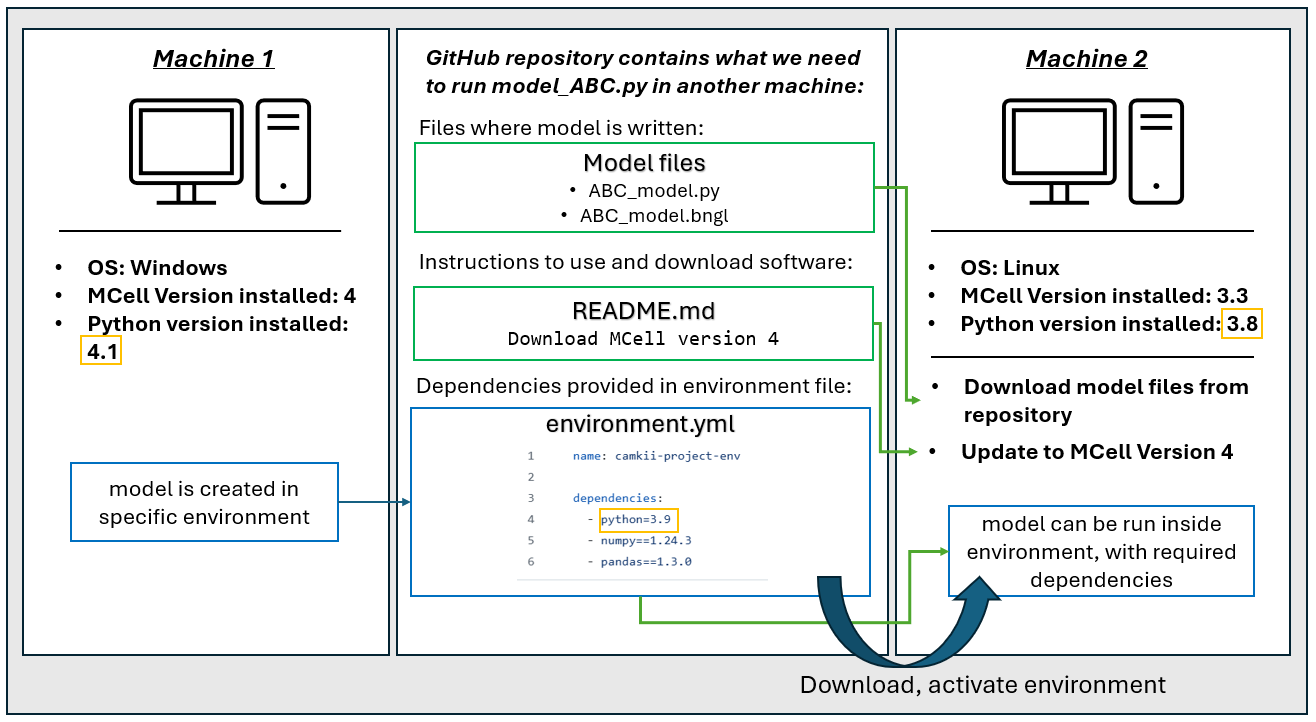
\includegraphics[keepaspectratio]{22-reproducibility-figures/environment.PNG}}

}

\caption[Computational Environments]{\label{fig-environment}As an
example of how environments work, the model is initially created on
Machine 1, which runs the Windows operating system, has MCell version 4
installed, and uses Python version 4.1. To ensure that the model can be
successfully executed on a different system, a dedicated computational
environment is set up, capturing all the necessary dependencies. The
environment setup and the model files are uploaded to a GitHub
repository. This repository can contain the environment.yml file listing
the required dependencies, including Python 3.9, NumPy, and pandas, as
well as the model files (ABC\_model.py and ABC\_model.bngl), and a
README.md file with instructions (such as downloading MCell version 4).
On Machine 2, which runs Linux, has MCell version 3.3, and Python
version 3.8, the user can, according to README instructions, update
MCell to version 4 and use the specified environment by activating the
environment.yml file. The model can be run within this contained
environment.}

\end{figure}%

\subsubsection*{Prepare for Errors}\label{prepare-for-errors}
\addcontentsline{toc}{subsubsection}{Prepare for Errors}

Regularly testing code is, unsurprisingly, helpful for ensuring reliable
and reproducible research. Throughout my PhD, I have incorporated
various testing strategies to improve the reliability of my code. One
key practice has been anticipating and preparing for errors, which has
helped me catch potential issues before they become major problems. This
is nothing ground-breaking but rather following good-practice coding,
such as readable, commented code, as explained above, having print
statements to know what the code is doing where and when, error handling
and creating validation steps throughout. For me, creating validation
steps involved carefully adding reactions one by one, running the
code,and checking whether the molecules were behaving within a
biologically plausible range. The aim was not to enforce exact expected
outcomes, which could introduce bias, but to ensure that results were
not wildly outside the bounds of what is reasonable given the known
biology. Importantly, when deviations from expected patterns did occur,
I treated these as potentially meaningful, since in a stochastic model
they can reflect emergent behaviours. I have also learned to validate my
code step by step through debugging
{[}\citeproc{ref-mccauley2008Debugging}{386}{]}, the process of
identifying, analyzing, and fixing errors or bugs in a program, to break
down how the code is working and pinpoint where things go wrong.
Additionally, I have used mock or dummy test models, such as the
(ABC\_model: https://github.com/Susana465/test\_ABC), to simplify
testing when the main model is too complex to easily trace errors.

\subsubsection*{Version Control}\label{version-control}
\addcontentsline{toc}{subsubsection}{Version Control}

Version control is a pillar of most, if not all, guides for reproducible
research {[}\citeproc{ref-turingwaycommunity2019TuringWayHandbook}{356},
\citeproc{ref-sandve2013Ten}{387}--\citeproc{ref-hamra2025Advancing}{391}{]}.
Version control is a method for tracking and managing changes to files
or projects over time. It allows you and your collaborators to monitor
modifications, review past edits, and restore previous versions if
needed. Using version control helps maintain a relatively organized and
traceable record of updates across different stages of development. This
is extremely helpful for times when I needed to check back on when and
where I did a specific change to my work, or when working
collaboratively to know who wrote what and when. In terms of
reproducibility, this means that version control helps with having clear
provenance of information {[}\citeproc{ref-hamra2025Advancing}{391}{]}.
As a result of using version control, I have made my life easier (and
potentially others in the future too) as I could track what version of
the code and data produced specific outputs, for example. As datasets
grow larger and more complex, by having a solid version control workflow
you are doing your future self (and collaborators) a huge favour.

There are various ways to implement version control
{[}\citeproc{ref-atkins2002Using}{392}--\citeproc{ref-hethey2013GitLab}{395}{]},
but I primarily use Git and GitHub
{[}\citeproc{ref-loeliger2012Version}{396}{]} ---partly because they are
widely adopted and partly because they were the tools introduced in the
version control courses I attended. With Git, each version update (or
``commit'') can include a message describing the changes made, such as
``changed value x=1 to x=2.'' This has made it much easier to track
modifications over time and follow the evolution of this project.
Version control is therefore, especially useful when sharing analyses,
as it ensures transparency, reproducibility, and auditability -key
aspects of good scientific practice.

\paragraph*{Gradual Development and
Validation}\label{gradual-development-and-validation}
\addcontentsline{toc}{paragraph}{Gradual Development and Validation}

The way I built the model for this project involved gradually developing
the code; for example, starting with CaMKII as a monomer, then a
hexamer, and finally a dodecamer. This step-by-step approach ensured
proof of concept and allowed me to develop the model incrementally,
building on solid, validated foundations before moving to the next
stage. Git's branching feature made this process much smoother, as it
let me work on different aspects of the model in separate lines of
development without affecting the main project. This meant I could
experiment, test, and refine changes in parallel workspaces, keeping the
main codebase stable until updates were ready to be merged. Further
details on model validation can be found in
Section~\ref{sec-validating-model}.

\paragraph*{Data Management}\label{data-management}
\addcontentsline{toc}{paragraph}{Data Management}

With this gradual development, the datasets evolved, variable names
changed, and file hierarchies were adjusted throughout. As a result,
managing large data outputs eventually became a challenge (see
Challenges in Version Controlling Data described by
{[}\citeproc{ref-turingwaycommunity2019TuringWayHandbook}{356}{]}). For
example, GitHub imposes a limit of 100MB per file, preventing the
storage of large files directly within the repository. Whilst Git can be
used for data versioning by installing tools like git-annex, Git LFS, or
git submodules, this means integration of more complex tools, which can
introduce accessibility issues for newcomers. For example, with a data
version control add-on tool like DataLad (which builds upon git and
git-annex (https://git-annex.branchable.com/)), users may be able to see
the files in the repository, but they won't be able to access or
download it directly, instead they would have to clone the entire
repository, which may be far from ideal. This added complexity can be a
barrier for those who are not familiar with the tools, potentially
hindering the ease of use for collaborative projects.

To address data versioning, I implemented various strategies. Firstly,
timestamping output files: I saved output files with timestamps rather
than overwriting them. This practice ensures that each file's creation
time is preserved, although it does not allow for version control of
those files. While this means any modifications to the files won't be
tracked automatically, the documentation clearly specifies that any
updates to the files should be reflected in the file names, maintaining
clarity and transparency. Secondly, I developed a simplified version of
the model, called the ABC\_model, which mirrors the workflow of the main
CaMKII\_dodecamer\_model. This model tracks fewer molecules (e.g., a + b
-\textgreater{} c) and produces less complex, smaller output files.
Although this doesn't address the version control of the primary model's
data, it is an effective tool for monitoring how outputs are generated
and understanding their structure during testing phases. Additionally, I
uploaded final outputs to a database: once the final, validated outputs
were produced, I uploaded them to a database for proper storage and
sharing. This step ensures that the final, reproducible data is securely
stored and accessible. Likewise, packing data output files into smaller
sized files (for example, zipping them), allows for data to be tracked,
albeit, sometimes this is not a viable solution because data may still
be too big.

\paragraph*{Quarto for Version-Controlled
Documents}\label{quarto-for-version-controlled-documents}
\addcontentsline{toc}{paragraph}{Quarto for Version-Controlled
Documents}

In addition to maintaining version control of the model(s), I also used
Quarto {[}\citeproc{ref-allaire2024Quarto}{397}{]}, an open-source
publishing system designed for scientific and technical writing. Quarto
enables the dynamic generation of various file formats, including
Markdown, LaTeX, HTML, PDF, and Word, all of which can be version
controlled. This functionality has been invaluable in creating a
structured, traceable workflow within a single, integrated system. By
leveraging Quarto's flexibility, I have been able to write my thesis in
Markdown, a highly intuitive and lightweight markup language, while
keeping individual .qmd (Quarto Markdown) files under version control.
Quarto then renders these files into my preferred output format,
including PDF, Word, LaTeX, among other formats. This approach has been
significantly more efficient than the previous ad-hoc method of manually
tracking document versions (e.g., final, final\_forreal,
final\_forreal2), which lacked transparency and made it difficult to
trace specific changes. With Quarto, I can use version control of the
files and precisely track modifications, review previous iterations, and
revert to earlier versions when necessary, greatly improving both the
organisation and reliability of my work.

\subsubsection*{Automation for Efficacy and
Sustainability}\label{automation-for-efficacy-and-sustainability}
\addcontentsline{toc}{subsubsection}{Automation for Efficacy and
Sustainability}

Beyond ensuring clarity, documentation, and reproducibility, automation
plays a key role in making code more sustainable. By automating
repetitive tasks, I reduce the likelihood of human error, save time, and
ensure consistency across different runs of the model. This is
particularly important when working with complex simulations, large
datasets, or high-performance computing (HPC) environments, where
manually setting up and executing processes can be inefficient and
error-prone.

One example of automation in this project is the use of scripts for
setting up environments and running simulations. Instead of manually
installing dependencies and configuring settings each time the model is
used, I have created scripts that automatically execute the necessary
commands to run the model, as well as provide computational environment
files that can be used to run the model in different machines. This
eliminates the risk of missing dependencies, ensures the correct
software versions are used, and reduces the setup burden for new users.
Additionally, I have automated data processing workflows to streamline
the handling of simulation outputs. Large-scale simulations generate
significant amounts of data, and manually processing these results would
be time-consuming and inconsistent. By writing reusable scripts for
tasks such as data cleaning, aggregation, and visualization, I ensure
that results are processed systematically and efficiently. This not only
saves time but also makes it easier to compare outputs across different
runs, improving the reproducibility of results.

\section{Reflections and Future
Steps}\label{reflections-and-future-steps}

As with most research projects, there are always opportunities for
refinement and further exploration. While I am pleased with the level of
effort and attention put into reproducibility throughout this work,
there are several directions in which this could be extended and
strengthened.

The model was reproduced at different stages of development and
successfully run on multiple machines, demonstrating practical
reproducibility. Although I have not included figures here, the
corresponding test runs, environment files, and outputs are fully
available in the accompanying GitHub repository, where they can be
directly inspected and re-executed by others to independently confirm
reproducibility.

Looking ahead, I am keen to extend this work through a formal
publication that includes a more comprehensive evaluation of how the
project aligns with FAIR and open science principles. A structured FAIR
assessment, such as the one proposed by Balaur et al.
{[}\citeproc{ref-balaur2025FAIRification}{398}{]}, could provide a
detailed appraisal of the reusability and transparency of the models
developed. In support of these reflections, I refer to the
reproducibility framework developed by Tiwari et al.~(2021). Based on
the rubric provided (see Figure~\ref{fig-tiwari-rubric}), I have scored
this project at 6.5 out of 8. As described throughout this chapter,
considerable effort has gone into meeting the majority of the quick
criteria proposed by
{[}\citeproc{ref-tiwari2021Reproducibility}{399}{]}.

\begin{figure}

\centering{

\pandocbounded{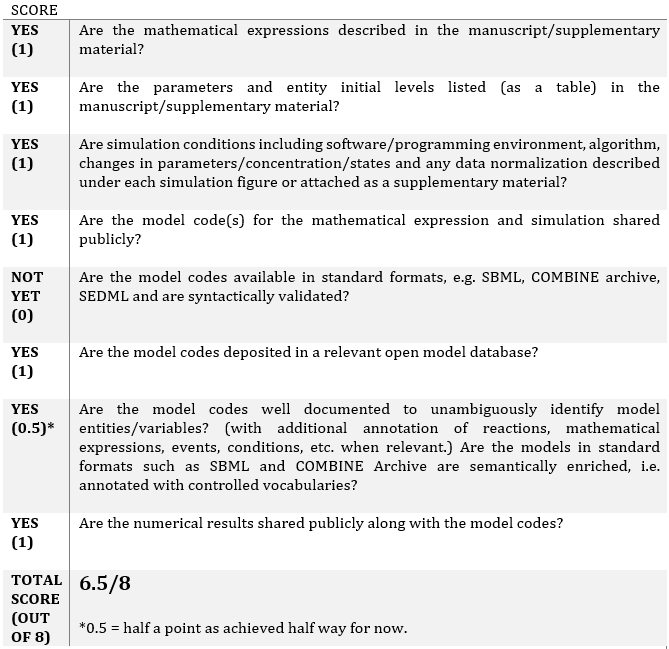
\includegraphics[keepaspectratio]{22-reproducibility-figures/tiwari-rubric.PNG}}

}

\caption[Reproducibility
Scorecard]{\label{fig-tiwari-rubric}Reproducibility Scorecard suggested
by {[}\citeproc{ref-tiwari2021Reproducibility}{399}{]}, adapted.}

\end{figure}%

One area still under development is the conversion of the model code
into standardised formats such as SBML, with the intention of submitting
it to a public repository for mathematical models of biological and
biomedical systems, such as BioModels
{[}\citeproc{ref-lenovere2006BioModels}{400},
\citeproc{ref-malik-sheriff2020BioModels}{401}{]}. BioModels requires
submissions to follow specific guidelines, which include the provision
of SED-ML (Simulation Experiment Description Markup Languag) files ---a
format used to describe the simulation experiments performed on
computational models, including details of the algorithms, tasks, and
outputs. Experimental data, simulation results, and associated metadata
can also be submitted in a COMBINE archive, a single container file that
brings together all relevant documents required to fully describe,
reproduce, and share a computational modelling project
{[}\citeproc{ref-bergmann2014COMBINE}{402}{]}.

With respect to the seventh criterion in the Tiwari et al.~(2021)
framework, I awarded a partial point. The model is well annotated, with
inline comments and supporting tables that describe variables and their
meanings, thus aiding interpretability. However, molecule and reaction
naming conventions, while consistent within the project, could benefit
from further simplification. This is a known challenge in computational
biology, where names must often strike a balance between being
human-readable and programmatically functional (see, for example,
discussions on standardised biological ontologies)
{[}\citeproc{ref-bodenreider2006Bioontologies}{403}--\citeproc{ref-fitzpatrick2022Validation}{405}{]}.

Overall, the limitations identified here present valuable opportunities
for growth and refinement, typical of any ongoing research effort.
Future steps represent an exciting part of the process that will enhance
the transparency, accessibility, and usefulness of the model for the
broader research community. By ensuring that models follow FAIR, open
principles we not only strengthen the scientific rigour of this PhD, but
also uphold the ethical responsibility of researchers to share their
work in a way that benefits the wider community. This is precisely what
is discussed next.

\section{Defining Ethical Science}\label{defining-ethical-science}

Open, reproducible and FAIR ideas are fundamentally linked to ethics, as
these practices ultimately promote more ethical and responsible research
by fostering transparency, integrity, and accountability
{[}\citeproc{ref-farrow2016Framework}{406},
\citeproc{ref-kushwaha2024Ethical}{407}{]}. No matter how efficient or
reproducible a study may be, its value is questionable if it causes harm
to a group of individuals. Likewise, recognizing biases and risks in our
research without providing the necessary resources for replication may
undermine the advancement of truly ethical and reliable research.

Here, we refer to ``scientific ethics'' as the principles and guidelines
that govern the behaviour of scientists in their work, and their impact
in wider society
{[}\citeproc{ref-rollin2006Science}{408}--\citeproc{ref-menapace2019Scientific}{410}{]}.
More broadly, ethics can be seen as a system of moral values and
principles that a particular society or community upholds
{[}\citeproc{ref-gensler2017Ethics}{411}{]}. Ethics can be understood as
a core aspect of moral philosophy -an area of study that, among other
things, seeks to differentiate between right and wrong. Viewing ethics
as the study of what constitutes appropriate or inappropriate behaviour
emphasizes its connection to action. Therefore, we can see how ethics is
relevant when considering the impact of actions and behaviours of
scientists throughout the research process. Recognizing this also
highlights the fundamental role of moral philosophy and ethics in
shaping how research impacts society.

Ethical standards and beliefs evolve over time, and as a result, so do
the ethical guidelines that govern scientific research
{[}\citeproc{ref-joyner2002Evolution}{412}--\citeproc{ref-macklin2008Standard}{414}{]}.
Practices that were once considered acceptable may no longer align with
contemporary ethical norms, just as certain current methodologies may be
deemed unethical in the future. Either way, throughout history,
including current times, there are numerous examples of scientific
research leading to significant ethical concerns and harmful
consequences {[}\citeproc{ref-garcia2022Thinkinga}{378},
\citeproc{ref-jackson2005Origins}{415}--\citeproc{ref-birhane2020Decolonising}{417}{]},
as discussed more in detail in the article included in
Chapter~\ref{sec-data-hazards-chapter}. I believe it is important to
recognise the heavy weight that science carries, of not only unethical
but also oppressive research that has undermined and hurt minoritised
groups and individuals throughout time. Unless we recognise where
scientific research stands and where it comes from, we cannot stop
repeating the same oppressive behaviours that may go unspoken or
unrecognised otherwise.

In a presentation I delivered in 2022, I provided several examples of
historical social biases that persist in scientific research, with a
focus on medicine, neuroscience and computer Science, including examples
of racism, sexism, ableism, and speciesism
{[}\citeproc{ref-garcia2022Thinkinga}{378}{]}. I define social bias as a
systematic and often unconscious prejudice or favouritism toward certain
groups over others, based on characteristics such as race, gender,
species, or other socially constructed categories. A good example of
embedded biases in science is given by
{[}\citeproc{ref-branch2022Discussionsa}{418}{]} as they eloquently
articulate how a desire to quantify and establish hierarchies among
organisms was not purely for scientific interest, but that there is
extensive evidence in the fact that the roots of evolutionary biology,
which serves as a baseline for many other disciplines like neuroscience,
are steeped in histories of white-supremacism, eugenics, and scientific
racism. They discuss the definition of the ``Not-So-Fit'', and how this
limits the diverse thought and investigative potential in biology. This
is important to recognise for this thesis, as I use hierarchies and
models of biology that are based on a historical context of how science
has reached its current status of knowledge.

\section{Why is this important?}\label{why-is-this-important}

Reflecting on the ethical history and potential future implications of
research helps to uphold accountability and minimise harm, as further
discussed in the Data Hazards Chapter~\ref{sec-data-hazards-chapter}. It
is the synergy of combining openness, reproducibility and ethics that
create research that shows integrity and enhances credibility
{[}\citeproc{ref-medicine2017Fostering}{419},
\citeproc{ref-zhaksylyk2023Research}{420}{]}. Thinking about
reproducibility can, in turn, help to think how you will share your
data, as well as where your own data has come from. Hence, reaching an
increased awareness of how data was sourced and its ethics and potential
biases. Working with ethics, philosophy, reproducibility and an openness
to discuss the wider context of where our research rests, may add time
to the research timeline, but can very much enrich a fuller and more
complex understanding of the shortcomings of our research and how to do
better moving forward. This is why I believe that continuous reflection
on ethical standards is essential, and why I have made a big emphasis on
reiterative reflection throughout this PhD.

As we have seen, creating research that takes into account openness,
reproducibility and ethical considerations offers benefits not only for
researchers but for society as a whole. Researchers can directly benefit
through increased visibility and citation rates, greater opportunities
for collaboration, and reduced waste of time and resources.
Additionally, fostering open scientific practices helps build a stronger
sense of community, in contrast to the traditionally competitive nature
of research. Embedding these considerations into research workflows can
enhance the credibility and reliability of scientific findings.
Furthermore, reflecting on the broader impact of research promotes
accountability and encourages proactive measures to mitigate potential
harm.

Beyond academic advantages, open, ethical, and reproducible research
contributes to more equitable knowledge dissemination. When data,
methods, and findings are openly shared, barriers to access are reduced,
enabling a wider range of researchers, institutions, and communities to
engage with and build upon existing work. This can drive innovation,
improve public trust in science, and ensure that research benefits can
be reaped by as many individuals as possible.

\subsection{A personal account: Where it
started}\label{a-personal-account-where-it-started}

Before turning to the technical discussion of Data Hazards in the
following chapter, I offer a brief personal account of how I came to
engage with these issues, alongside a poster I developed to capture the
key questions and reflections that have shaped my thinking throughout
this PhD.

A common experience in my academic career has been the limited focus on
the social dimensions of ethics in the research I conduct. As I became
aware that much of the research I conduct is based on biased views of
how the world works
{[}\citeproc{ref-tjeltveit2015Appropriately}{421}--\citeproc{ref-ross2020Everyday}{423}{]},
I developed a keen interest in examining the biases within my own work.

My position as a woman, an immigrant in the UK, and someone from a
working-class background has deeply shaped my experience in academia. It
has influenced how I am perceived, the hurdles I've had to overcome, and
the opportunities available to me. Over time, these experiences have led
me to care deeply about the inequalities I kept encountering. At the
same time, I also acknowledge the privileges I hold, being perceived as
white, European, and a student at a prestigious university. These
intersecting experiences of marginalisation and privilege have shaped
and motivated my commitment to critically examine implicit biases within
society and strive for a more equitable and accessible research process.

My focus on addressing biases in my research made me realise the need
for greater reproducibility and accessibility to ensure open, meaningful
dialogues, and progress. The initial bias I encountered was the
assumption that ``there is no need to account for social bias in my
research'', because one might think my research topic is neutral at
first glance: computer simulations of proteins does not scream a need
for ethical considerations, mainly because we are not directly using
animals, human or non-human.

In an effort to challenge the initial notion that my project does not
require ethical considerations, I began exploring how others were
thinking about bias and reproducibility. This led to the creation of a
detailed (though wordy) poster, which framed my PhD journey as a series
of milestones. I presented this poster at the COMBINE and ICSB 2022
conferences {[}\citeproc{ref-romangarcia2022Biasa}{424}{]}, where I
shared how I address bias and reproducibility in my own work, and
encouraged researchers at various stages of their careers to reflect on
these aspects in theirs. A common concern raised during these
discussions was the additional time and effort required to make research
fully reproducible. While it is true that ensuring reproducibility can
increase an individual's workload and extend the research timeline, it
ultimately proves more efficient in the long run. By making research
accessible, well-documented, and easy to build upon, future researchers
are better equipped to continue and expand on existing work, reducing
redundancy and advancing scientific progress more effectively.

At each milestone proposed in the poster, I present potential biases
that could influence the work, along with tools to either mitigate or
highlight them. At the same time, I recognised that for my PhD to be
truly ethical, it needed to prioritise both reproducibility and
accessibility. To reflect this, I organised the questions I had been
grappling with into different sections of the research process. All of
this is documented in a publicly available GitHub repository
{[}\citeproc{ref-romangarcia2022Biasa}{424}{]}.

For instance, during the design of the computational model I use, I
consider questions such as: Who is my data including or excluding? What
assumptions am I making? To what extent am I simplifying? In my
research, I work mostly with data from non-human animals. A common
assumption in the field is that findings from experiments on mice can be
extrapolated to humans. However, it is essential to acknowledge that
this remains an assumption, not a certainty. Similarly, my work often
involves explaining memory and learning in highly simplified terms,
typically focusing on specific molecular mechanisms. Yet, these
processes are inherently complex, and we do not fully understand all
their nuances. Recognising these limitations is crucial for maintaining
scientific integrity and ensuring that findings are interpreted within
their appropriate context (see Figure~\ref{fig-posterPhDjourney} for
resources I used).

These questions around data provenance and the ethical dimensions of my
research are explored in greater depth in the next section, where I
introduce and explore the Data Hazards framework (see
Chapter~\ref{sec-data-hazards-chapter}). This framework encourages
researchers to critically assess not only the potential risks and
limitations of their work, but also how it might be used in future, and
what biases it could be perpetuating. Reflecting on these concerns
shaped the design of my computational model and prompted a broader
engagement with the ethics and reproducibility of research in
neuroscience. This line of thinking ultimately led to the development
and publication of the paper included in the following chapter ``Data
Hazards as an Ethical Toolkit for Neuroscience''
{[}\citeproc{ref-garcia2025Data}{381}{]}.

\begin{figure}[h]

\centering{

\href{https://github.com/Susana465/Bias-and-Reproducibility-Poster/blob/main/20221006_poster_phd_journey.jpg}{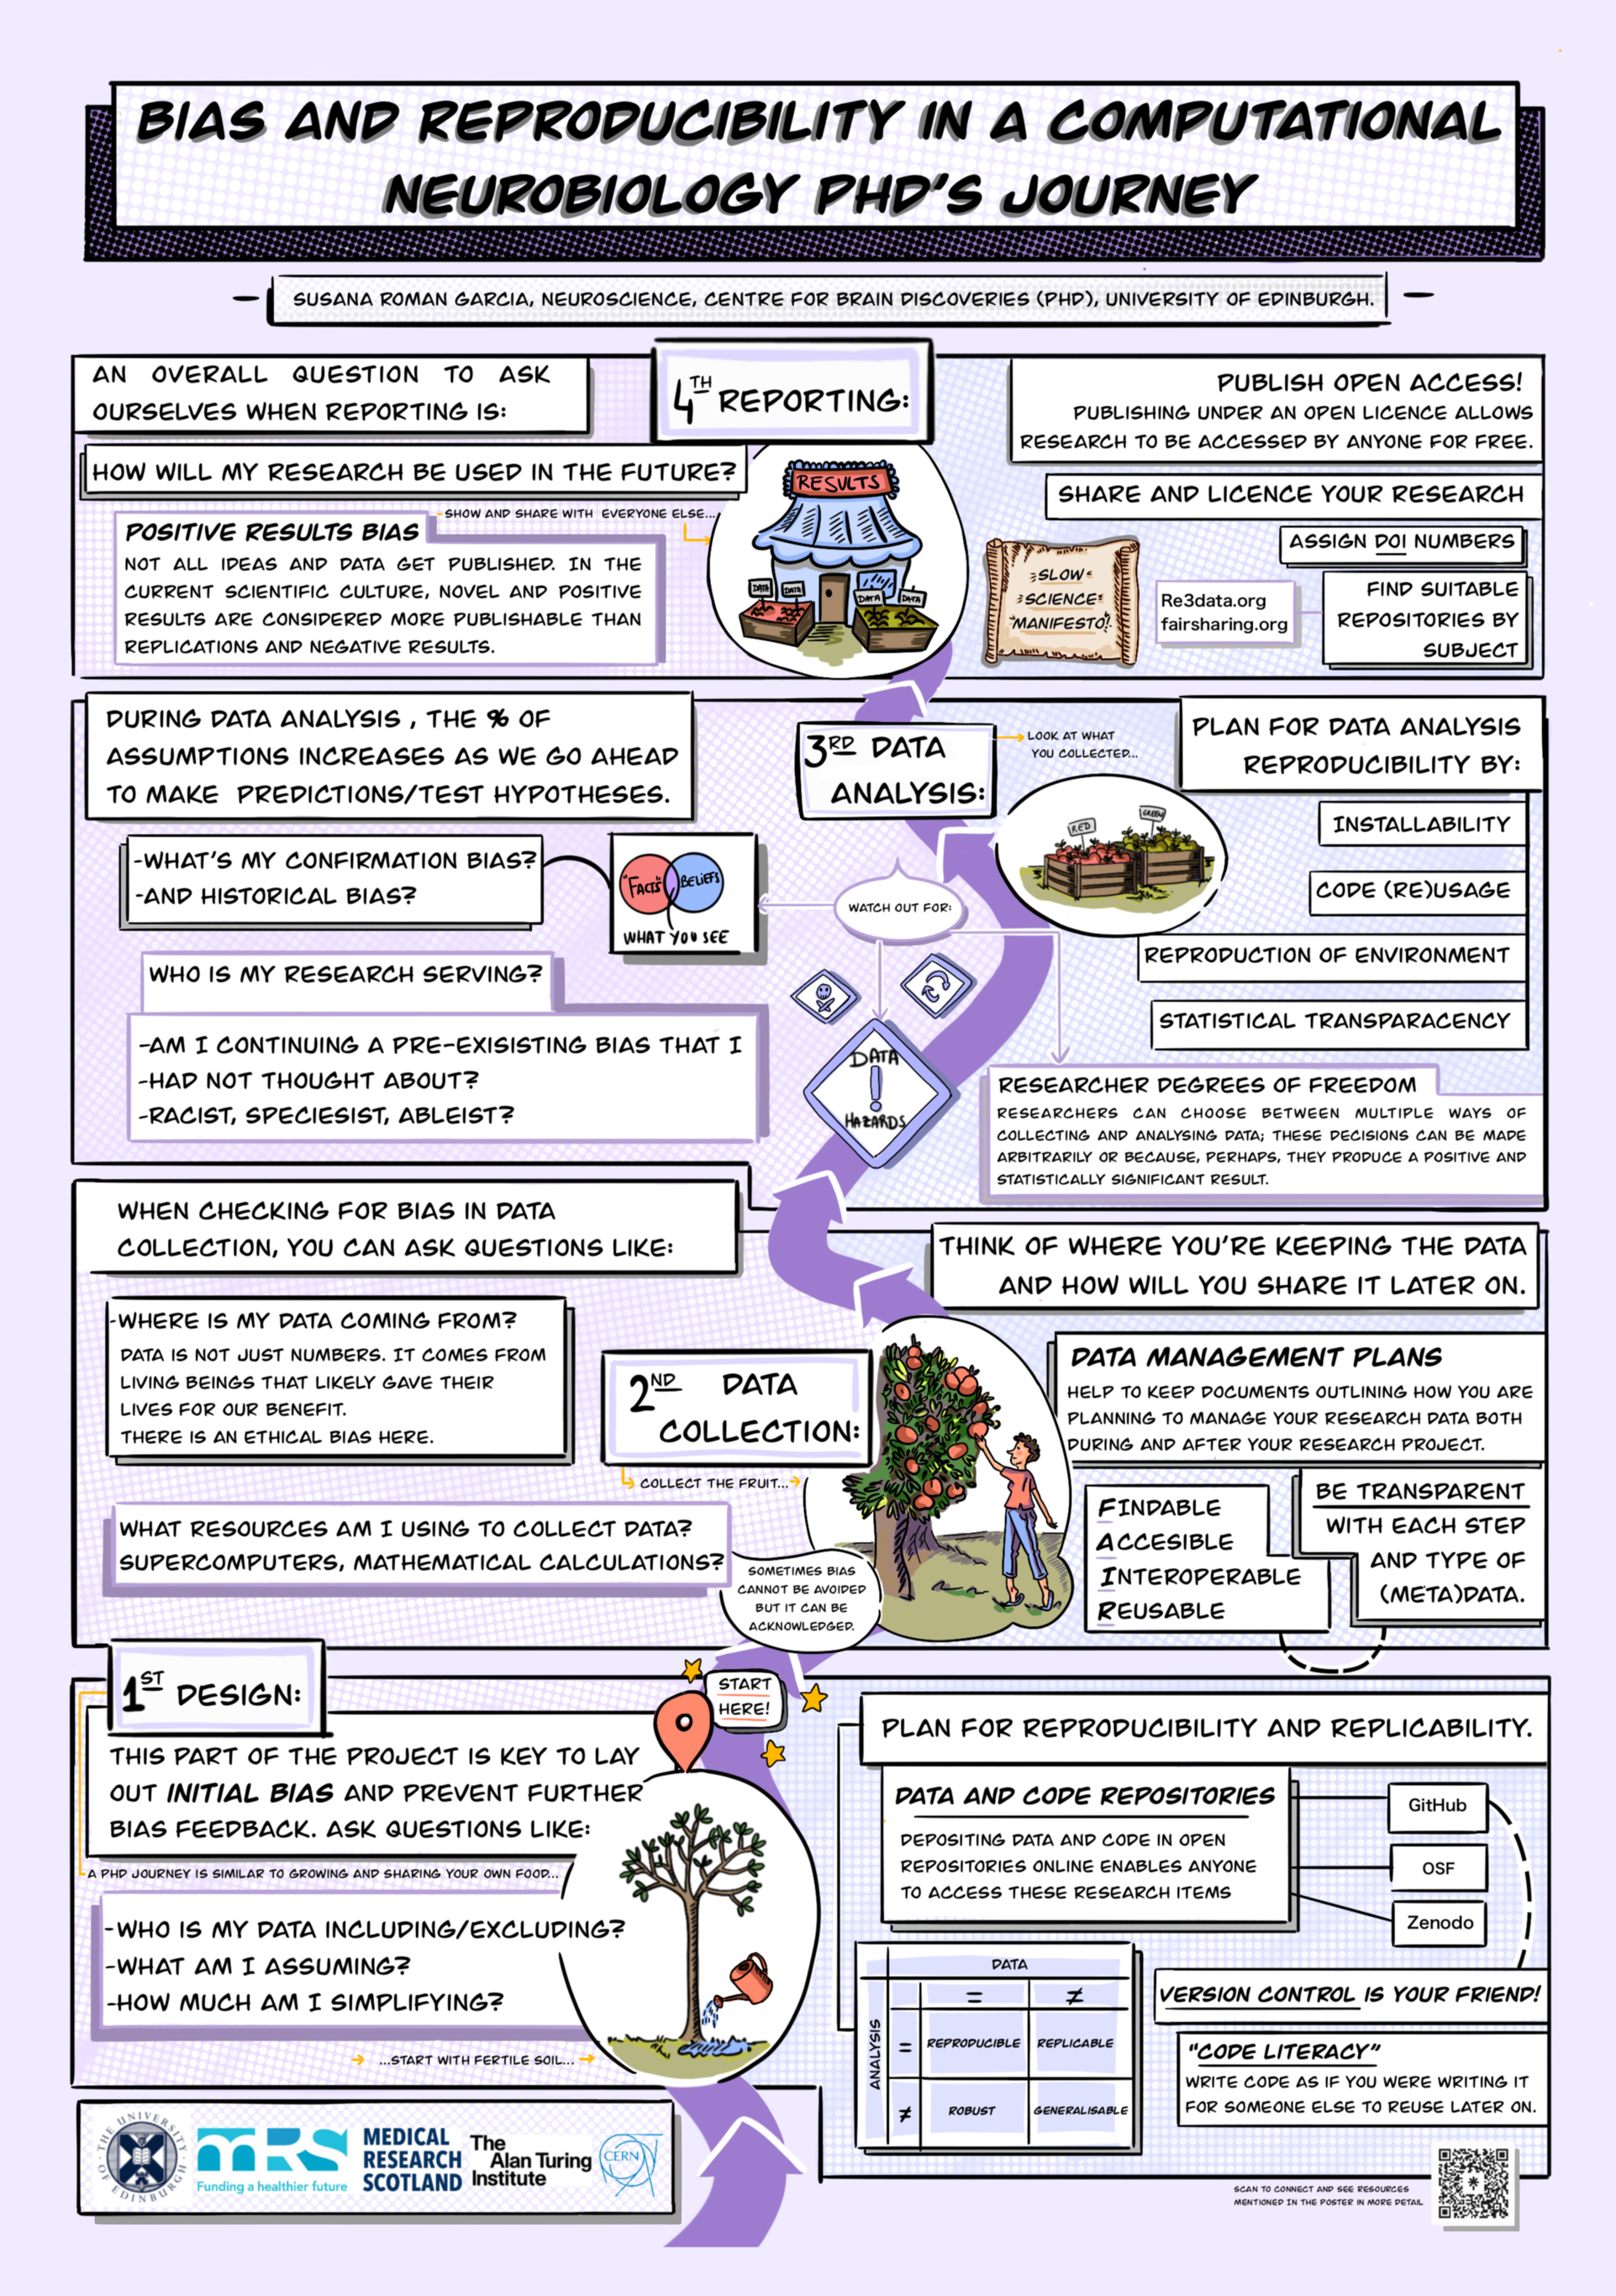
\includegraphics[width=5.20833in,height=\textheight,keepaspectratio]{22-reproducibility-figures/20221006_poster_phd_journey.jpg}}

}

\caption[Poster about bias and
reproducibility]{\label{fig-posterPhDjourney}Poster about bias and
reproducibility, showing research cycle as a journey which starts with
design, then data collection, data analysis and final reporting, and
compares this through images to growing an apple tree, collecting the
apples and then selling them.}

\end{figure}%

\bookmarksetup{startatroot}

\chapter{A Case Study in Ethical Reflection: Data Hazards in this
PhD}\label{sec-data-hazards-chapter}

As discussed in more detail below, the Data Hazards initiative was
developed as a community-driven, shared vocabulary to identify and
address risks and potential harms in data science
{[}\citeproc{ref-zelenka2023Data}{425}{]}. This project aims to mitigate
risks by helping researchers recognize potential ethical challenges that
may not have been initially considered and explore strategies for
addressing them. While data scientists are typically trained to solve
technical problems, ethical considerations are often overlooked. The
Data Hazards framework is designed to support reflection during the
research cycle, helping researchers anticipate and address nuanced
ethical issues such as bias, societal impact, and philosophy. At the
same time, the framework can serve as a ``disclaimer'' or ``warning''
allowing researchers to communicate to readers which Data Hazards may be
relevant to a project, and to highlight ethical considerations or
potential risks in publications when appropriate. The Data Hazards
project seeks to foster a cultural shift in research by encouraging a
wider adoption of ethical considerations within the science community,
promoting a more responsible and socially aware approach to scientific
work.

As part of my ongoing effort to assess the broader implications of my
research, I encountered the Data Hazards Project in 2021. Since then, I
have progressively applied the Data Hazards framework to my PhD
research. In addition to incorporating Data Hazards into my own
research, I have facilitated several workshops on the topic
{[}\citeproc{ref-roman-garcia2022Data}{426}{]}. In 2023, I co-organised
and co-hosted a one-day symposium focused on Data Hazards, ethics, and
reproducibility. Furthermore, I co-authored a chapter on Data Hazards to
The Turing Way handbook
{[}\citeproc{ref-turingwaycommunity2019TuringWayHandbook}{356}{]}.

The work that ultimately led to the development of the paper ``Data
Hazards as an Ethical Toolkit for Neuroscience'' was preceded by an
earlier collaboration with the Data Hazards team. As part of this, I
designed a poster for AI UK 2023 that followed the methodology outlined
in Method 1 of the {[}\citeproc{ref-romangarcia2023Data}{379}{]}. This
poster served as an interactive tool, enabling reflective discussions
with conference attendees who were invited to engage by selecting Data
Hazard labels they felt were applicable to my PhD project
(Figure~\ref{fig-barchart}).

\begin{figure}[H]

\centering{

\pandocbounded{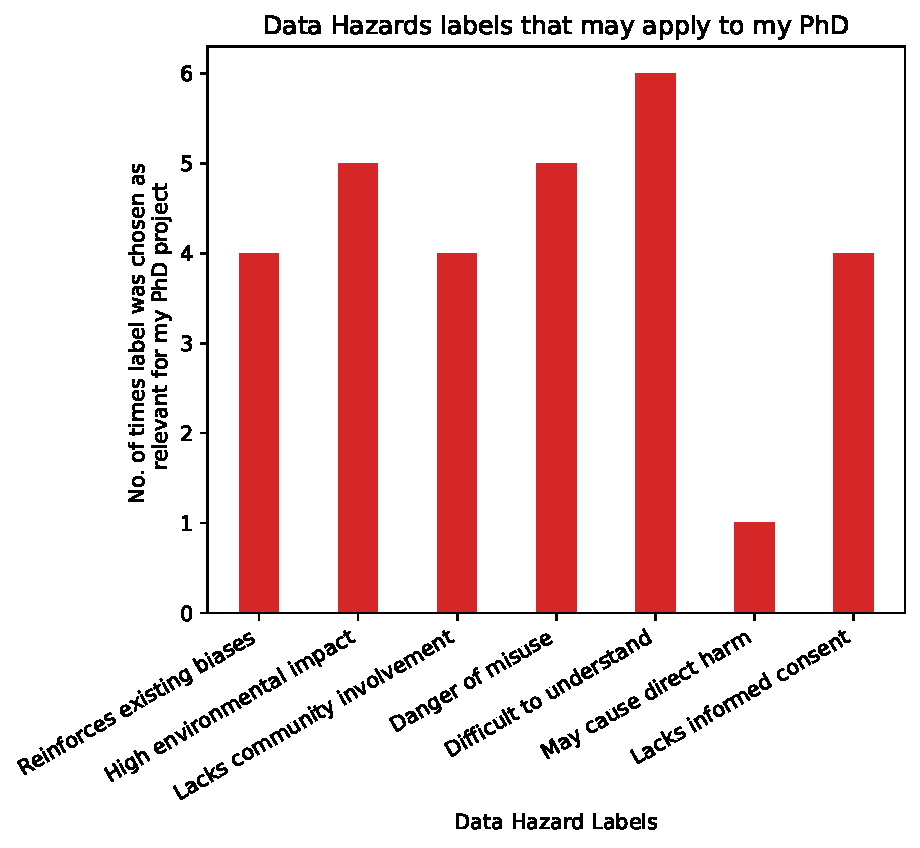
\includegraphics[keepaspectratio]{20-data-hazards_files/figure-pdf/fig-barchart-output-1.pdf}}

}

\caption[Data Hazards labels chosen by conference
attendees.]{\label{fig-barchart}Data Hazards labels that may apply to my
PhD. Each number indicates the total number of times a given Data Hazard
label was selected by conference attendees visiting the poster.
Attendees were invited to select any labels they felt were applicable,
so not every label was chosen by every attendee. From poster presented
at AI UK 2023, see details
\href{https://github.com/Susana465/DH_Project_CaseStudy}{here}.}

\end{figure}%

Interestingly, not all labels were chosen as applicable to my project
(Figure~\ref{fig-barchart}). Only 6 of the 11 current labels were chosen
as relevant, with ``difficult to understand'' being the most prevalent
one, chosen by 6 people. High environmental impact and danger of misuse
follow in closely with 5 people having chosen these ones. Of course
these numbers are small and hold, more than anything, illustrative value
as to how and why people may think certain labels apply to a project.
Difficult to understand'' label was chosen the most, followed by ``high
environmental impact'' and ``danger of misuse''. Throughout the
discussions, each person --- myself included --- brought their own
assumptions about which issues mattered more or less and why.
Disagreements around the application of the Data Hazard labels continued
during the follow up, in-depth collaborative work for the paper
presented below. While consensus wasn't always reached, these
discussions gave rise to meaningful conversations about the ethical
dimensions of the project.

I include these results not as definitive data, but to show the kind of
reflective, participatory work that led up to the paper. This approach
embodies the core aim of the Data Hazards project: to create space for
collaborative dialogue, invite critique, and support researchers in
actively thinking through the ethical implications of their work.

All of this work culminates with this PhD and the paper I present below,
where we extend the application of the Data Hazards framework to the
field of Neuroscience, exploring how these hazard labels can highlight
ethical challenges in computational modelling, specifically focusing on
my PhD as a case study. The following paper demonstrates how I have
identified risks of my work as well as the efforts taken to mitigate
them.

The development of this chapter and its associated publication was a
collaborative effort, and I would like to acknowledge the contributions
of each co-author using the Contributor Roles Taxonomy (CRediT)
(https://credit.niso.org/):

\begin{itemize}
\item
  Nicola Romanò contributed to the conceptualization of the work,
  provided supervision, and was involved in both the original drafting
  and reviewing and editing of the manuscript.
\item
  David C. Sterratt supported the conceptualization and provided
  supervision, as well as contributing to the review and editing of the
  manuscript.
\item
  Melanie I. Stefan was involved in the conceptualization, secured
  funding, provided supervision, and contributed to both the original
  drafting and reviewing and editing of the manuscript.
\item
  Nina Di Cara contributed to conceptualization, methodology
  development, and participated in reviewing and editing the manuscript.
\item
  Ceilidh Welsh was involved in the original drafting, reviewing and
  editing, and also contributed to conceptualization, funding
  acquisition, and visualisation (including the graphical abstract).
\item
  I, Susana Román García, contributed to the original drafting,
  reviewing and editing, conceptualization, funding acquisition, and
  visualisation (graphical abstract). I also played a key role in
  project administration, overseeing the execution and coordination of
  the paper.
\end{itemize}

I am deeply grateful to all co-authors for their collaborative spirit,
critical insights, and valuable contributions to both the paper and the
thinking that shaped this chapter.

\newpage
\newgeometry{top=0.5in, bottom=1in, left=0.5in, right=0.5in}

\pagestyle{plain}

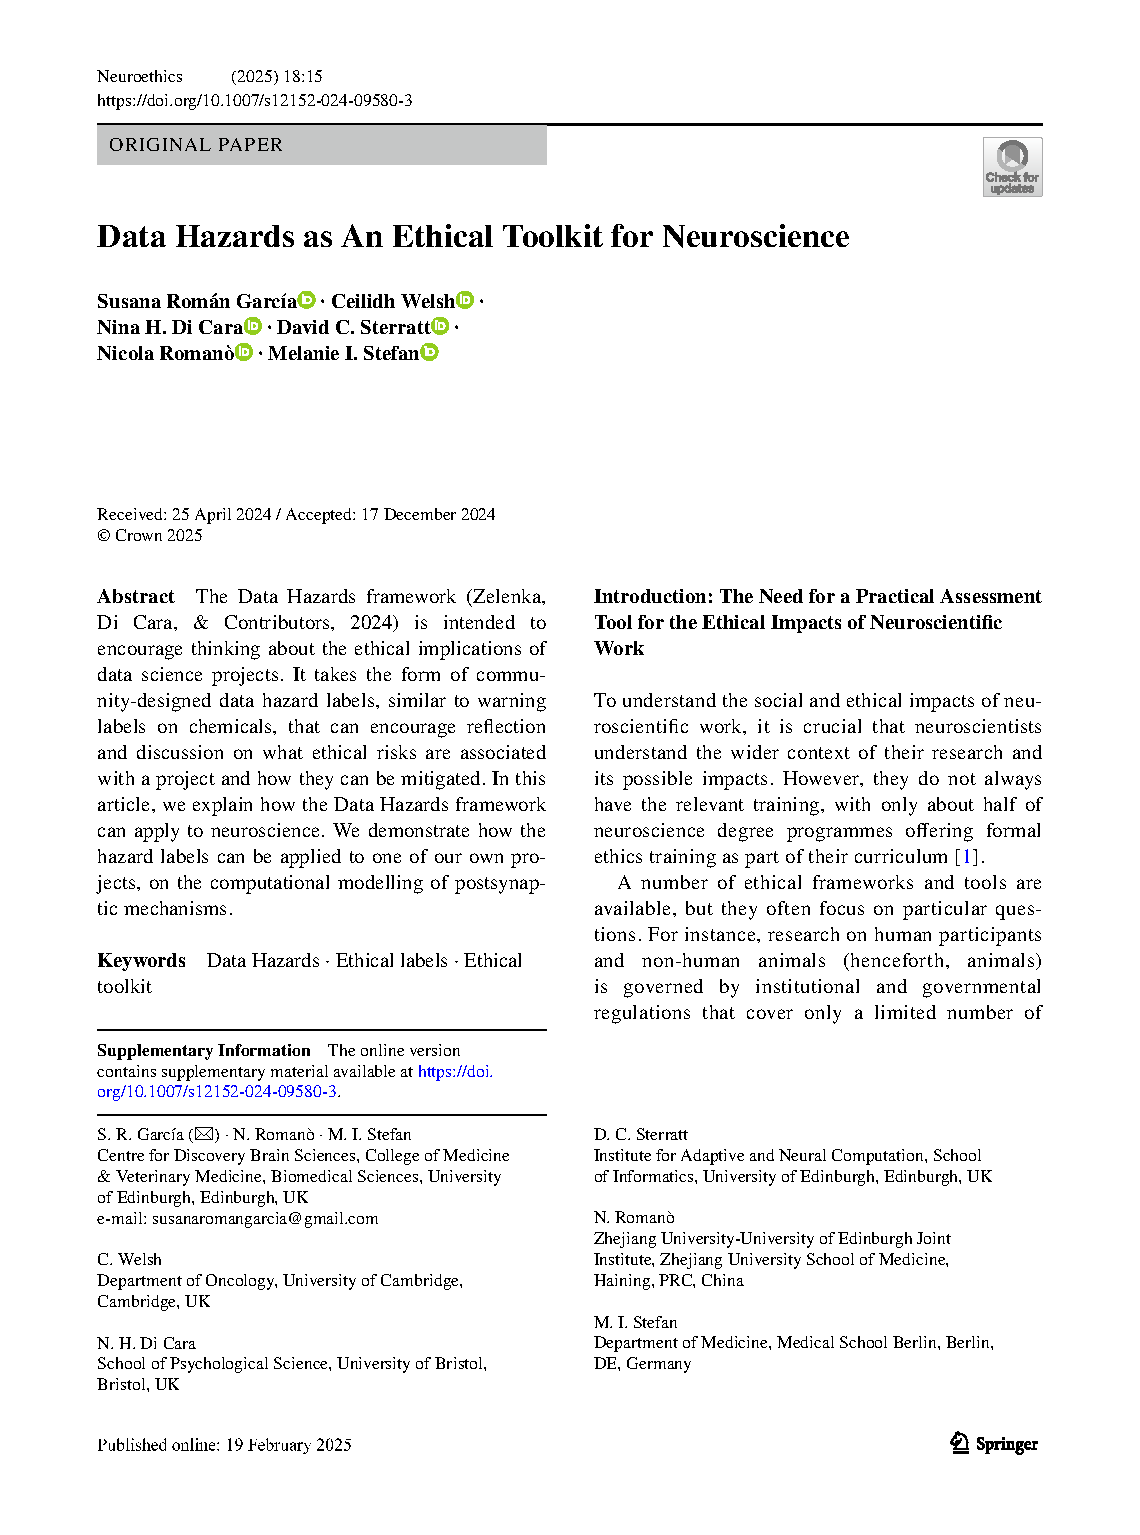
\includepdf[pages=-,pagecommand={\thispagestyle{plain}}]{neuroethics_paper.pdf}

\newpage 
\restoregeometry

\section*{Conclusion}\label{conclusion}
\addcontentsline{toc}{section}{Conclusion}

\markright{Conclusion}

This chapter has detailed my journey with the Data Hazards framework,
from initial engagement and community-driven activities to the
co-authorship of a publication applying the framework within
Neuroscience. Through workshops, symposiums, and collaborative writing,
I've sought to embed ethical reflection into the core of my research
practice. The culmination of these efforts is the paper ``Data Hazards
as an Ethical Toolkit for Neuroscience'', which not only applies the
framework to my PhD research but also proposes Data Hazards to better
suit the nuances of ethical discussions and risks in Neuroscience. This
work demonstrates how a PhD project such as this one can create space
for critical reflection on the potential consequences of scientific
research, and contribute to improving research integrity more broadly.

\bookmarksetup{startatroot}

\chapter{\texorpdfstring{\emph{In Silico} Model of CaMKII, NMDARs, and
Associated Signalling
Molecules}{In Silico Model of CaMKII, NMDARs, and Associated Signalling Molecules}}\label{sec-model-description}

Numerous computational models of CaMKII dynamics have been developed
over the past decade to look at different interactions of CaMKII and its
substrates or binding partners at varying levels of detail
{[}\citeproc{ref-pharris2019Multistate}{185},
\citeproc{ref-holmes2000Models}{427}--\citeproc{ref-bartol2024Spatial}{436}{]}.
Many of these models center on the binding of calcium to calmodulin
(CaM) and the subsequent formation of the CaM-CaMKII complex. While
these studies provide a good foundation for understanding CaMKII
dynamics, the models either focus solely on temporal dynamics without
considering geometry, or explore both spatial and temporal dynamics but
do not model CaMKII as a multimeric molecule. Some models do account for
CaMKII as a multimeric dodecamer
{[}\citeproc{ref-pharris2019Multistate}{185},
\citeproc{ref-ordyan2020Interactions}{435},
\citeproc{ref-bartol2024Spatial}{436}{]} but do not focus on its
interactions with NMDARs. To my knowledge, this research is novel in the
field, as it incorporates all these aspects: modeling CaMKII as a
dodecamer, examining spatiotemporal dynamics, and focusing specifically
on the CaMKII/NMDAR complex.

The research carried out in this PhD project follows recent studies
{[}\citeproc{ref-pharris2019Multistate}{185},
\citeproc{ref-ordyan2020Interactions}{435},
\citeproc{ref-bartol2024Spatial}{436}{]} that have looked at CaMKII as a
dodecamer to study its autophosphorylation and spatiotemporal regulation
in postsynaptic dendrites using BioNetGen and MCell. Incorporating
spatial, temporal, and multimeric aspects is crucial because these
dimensions fundamentally shape the behaviour of molecular complexes like
the CaMKII/NMDAR interaction. Spatial dynamics can reveal how the
molecules interact within different cellular regions; CaMKII
phosphorylation levels, as well as its functions have been shown to
differ depending on its subcellular localization
{[}\citeproc{ref-davies2007ACaMKII}{437}{]}. Temporal dynamics are
important to understand how CaMKII/NMDAR interactions evolve over time.
The duration and timing of CaMKII activation influence whether synaptic
changes are transient or long-lasting, affecting the induction and
maintenance of LTP and LTD.

The overarching objective of this PhD research is to investigate how
CaMKII and NMDARs interact within the postsynaptic dendrite following
calcium entry, using reproducible computational models. These
interactions are central to synaptic plasticity, as CaMKII activation
and its association with NMDARs play key roles in regulating the
molecular mechanisms underlying learning and memory. Understanding these
processes in greater detail can provide insight into how synaptic
strength is modified at the molecular level.

The research here is therefore structured around a series of specific
aims, investigated through three versions of a CaMKII/NMDAR model, one
wild type model and two mutant versions. The following section details
how the wild-type (WT) model was constructed. The two mutant (MT) models
differ only in a single modification each: one in which CaMKII cannot
phosphorylate at T286, and another in which CaMKII is unable to bind to
NMDARs. These mutations were implemented by setting the reaction rates
corresponding to CaMKII autophosphorylation and CaMKII--NMDAR binding,
respectively, to zero.

\section{Previous work}\label{previous-work}

Several multi-state models of CaMKII have been proposed, each differing
in focus and scope from the present one
{[}\citeproc{ref-pharris2019Multistate}{185},
\citeproc{ref-holmes2000Models}{427}--\citeproc{ref-bartol2024Spatial}{436}{]}.
Notably, there are multiple models by Stefan et al.
{[}\citeproc{ref-stefan2008Allostericd}{432},
\citeproc{ref-stefan2011MultiStage}{433}{]} on CaMKII which explore the
dynamics between CaMKII and CaM using Stochsim simulator
{[}\citeproc{ref-lenovere2001StochSim}{438}{]} which does not account
for spatial effects, unlike MCell. These computational models provide
insights into the mechanisms of calcium binding to CaM and the
subsequent interaction with CaMKII, influencing the kinase's activation,
phosphorylation, and opening and closing dynamics. Notably,
{[}\citeproc{ref-pharris2019Multistate}{185}{]} published a model that
specifically examines the dynamics of CaMKII in relation to CaM using
MCell. However, this study was conducted using MCell 3.3, which did not
support the diffusion of multi-state molecules. In this model, CaMKII
was represented as a dodecamer, though not using BNGL, and the
holoenzymes themselves were non-diffusing. Instead, the authors
implemented a model in which CaM could diffuse and interact with a
non-diffusing multi-state representation of CaMKII.

{[}\citeproc{ref-ordyan2020Interactions}{435}{]} employed a BioNetGen
rule-based modelling approach using Monte Carlo methods, similar to the
present study, to investigate how \(\mathrm{Ca^{2+}}\) signals influence
CaMKII phosphorylation dynamics within the PSD. Their work primarily
focuses on the interactions between CaM and the scaffolding molecule
Neurogranin (Ng) in regulating CaMKII dynamics. However, their study
does not investigate the crucial interaction between CaMKII and NMDARs.

More recently, {[}\citeproc{ref-bartol2024Spatial}{436}{]} have
published a study using the same version of MCell 4 as the model used in
this PhD. They use particle-based stochastic simulations in MCell4 to
model the activation of CaMKII by \(\mathrm{Ca^{2+}}\) flowing through
NMDARs within a postsynaptic spine. Their spatiotemporal model simulates
CaMKII as a dodecamer with calcium influx through NMDARs, yet they do
not directly examine interactions between NMDARs and CaMKII.

Each of these models represents a step towards the development of the
present study, which advances the field by explicitly modelling CaMKII
as a dodecamer that directly interacts with NMDARs on the surface of the
postsynaptic dendrite.

\section{Model Description}\label{model-description}

In this model, CaMKII is represented as a dodecamer using BioNetGen
Section~\ref{sec-camkii-as-dodecamer}. The model simulates its diffusion
over time and space within a postsynaptic density (PSD) volume. Other
molecules involved in the system include calcium, CaM, PP1, and NMDARs.
The following sections provide a detailed breakdown of how these
reactions are modelled, highlighting their biological relevance.

\subsection{Molecule concentrations, localization and cell
volume}\label{molecule-concentrations-localization-and-cell-volume}

All molecules (except NMDARs which are surface molecules) are released
from inside the cell to interact with each other. Molecules are released
as discrete molecule numbers. Concentrations can be calculated as shown
below in Equation~\ref{eq-molec-concentrations-calc}, where we begin
with the number of molecules \(N\) and convert it to moles using
Avogadro's number \(N_A\). Next, we account for the volume in cubic
micrometers, represented as \(V \, (\mu \text{m}^3)\). This equation
gives us concentration in Molar.

\begin{equation}\phantomsection\label{eq-molec-concentrations-calc}{
N \, \text{molecules} \times 
\frac{1 \, \text{mol}}{N_A \, \text{molecules}} \times 
\frac{1}{V(\mu \text{m}^3)} \times 
\frac{V \, (\mu \text{m}^3)}{V \, (\text{L})} = 
Concentration \, (\text{M})
}\end{equation}

The example calculation below considers an initial release of 10000
molecules and a dendritic volume of 0.5 µm³
(Equation~\ref{eq-molec-concentrations-calc-example}).
\begin{equation}\phantomsection\label{eq-molec-concentrations-calc-example}{
1*10^{4} \text{molecules} \times 
\frac{1 mol}{6.023*10^{23} \text{molecules}} \times 
\frac{1}{0.5 \, \mu \text{m}^3} \times 
\frac{1  \, \mu \text{m}^3}{10 ^{-15} \text{L}} =
3.32*10^{-6} \text{M}
}\end{equation}

CaMKII is modelled as a dodecameric molecule, which is biologically
accurate. The model contains the following molecules: CaM, PP1, CaMKII,
NMDARS, and calcium, each defined with distinct molecular binding sites
(Figure~\ref{fig-molecule-concentrations}). \(\mathrm{Ca^{2+}}\) ions,
CaM, CaMKII and PP1, are initially released inside the cytosol, and
NMDARs are released as cell surface molecules. Interactions between
calcium, CaM, and the other molecular species, can be found in
Figure~\ref{fig-tbl-1}.

\begin{figure}[H]

\centering{

\pandocbounded{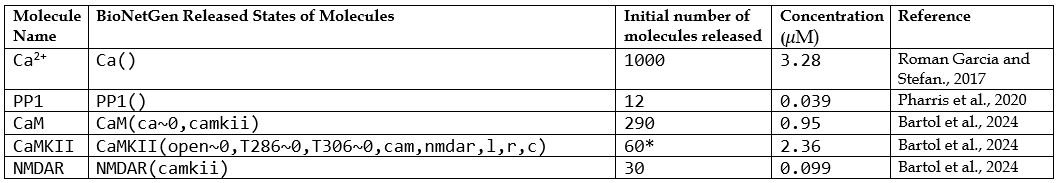
\includegraphics[keepaspectratio]{30-methods-figures/molecule-concentrations.PNG}}

}

\caption[Molecule concentrations in the
model]{\label{fig-molecule-concentrations}Molecules released into the
model, including their defined possible states specified in BioNetGen.
Concentrations were calculated using
Equation~\ref{eq-molec-concentrations-calc}, based on a simulation
volume of 0.50588 \(\mu\text{m}^3\). *Note: 60 CaMKII holoenzymes, each
comprising 12 subunits, correspond to a total of 720 subunits (60 ×
12).}

\end{figure}%

\subsection{Biological Plausibility}\label{sec-biological-plausibility}

While care was taken to compare model outputs with known biological
processes described in the literature and supported by experimental
data, this type of comparison is inherently complex. Different models
capture different aspects of biological systems, and even subtle
variations in assumptions or parameter choices can lead to divergent
behaviours. As such, the evaluation of biological plausibility should be
interpreted with caution; it provides useful insight, but not definitive
validation. The process of matching simulated outputs---such as
concentration profiles and reaction kinetics---to literature values is
valuable, yet inherently limited by the variability and uncertainty
present in both modelling and experimental data.

In the model presented here, reactions of cytoplasmatic molecules
specified in BNGL, were placed into the geometry of a postysnaptic
dendritic spine with a volume of 0.50588 \(\mu\text{m}^3\), which
matches the volume chosen by
{[}\citeproc{ref-ordyan2020Interactions}{435}{]} in their model of
CaMKII in the PSD and is within ranges of spine volume of 0.004 to 0.6
μm3 in hippocampal CA1 neurons (Harris et al., 1989). Moreover, Tonnesen
et al. {[}\citeproc{ref-tonnesen2018SuperResolution}{439}{]} report a
median spine volume of 0.1 \(\mu\text{m}^3\), with some spines reaching
up to 0.5\textasciitilde{}\(\mu\text{m}^3\). As such, a volume of 0.5
\(\mu\text{m}^3\) is within physiologically observed bounds, albeit on
the higher end of the range.

The molecular concentrations used are also within biologically plausible
ranges. For example, the initial release of 1000 \(\mathrm{Ca^{2+}}\)
ions corresponds to a concentration of 3.28\,\(\mu\text{M}\).
Fluorescent \(\mathrm{Ca^{2+}}\) indicator studies show resting
intracellular \(\mathrm{Ca^{2+}}\) concentrations between
0.05--0.1\,\(\mu\text{M}\), with increases up to 100-fold during
stimulation {[}\citeproc{ref-brette2012Handbook}{440},
\citeproc{ref-zheng2018Monitoring}{441}{]}. Therefore, the calcium
concentrations used are within ranges of stimulated neuronal activation.
I discuss this further in the discussion section and future steps of the
model.

With respect to CaMKII, concentrations of CaMKIIα subunits have been
reported to range between 5 and 100\,\(\mu\text{M}\) in neuronal
dendrites
{[}\citeproc{ref-lee2009Activation}{442}--\citeproc{ref-otmakhov2012Measuring}{444}{]}.
NMDARs are typically found at approximately 10 to 100 receptors per
synapse {[}\citeproc{ref-petralia2012Distribution}{445}{]}. In the
present model, the concentrations of CaMKII and NMDARs are positioned at
the lower end of these reported ranges, primarily due to the relatively
large spine volume modelled. Specifically, we include 290 CaMKII
subunits (equivalent to 2.36\,\(\mu\text{M}\)) and 30 NMDARs
(0.099\,\(\mu\text{M}\)). Although the concentration of CaMKII in this
model is on the lower end of reported values, this choice remains valid
given the larger spine volume incorporated in the model, which dilutes
the concentration of CaMKII while maintaining a reasonable estimate for
its overall abundance
{[}\citeproc{ref-lee2009Activation}{442}--\citeproc{ref-otmakhov2012Measuring}{444}{]}.
Furthermore, the number of NMDARs in the model is within the reported
range, reinforcing the biological relevance of the simulation. The
limitations of these parameter choices and potential future directions
for refining this model are further discussed in the Future Directions
section.

PP1 concentrations in neurons are typically reported between 1
\(\mu\text{M}\) and 10 \(\mu\text{M}\)
{[}\citeproc{ref-cohen2002Protein}{446}{]}, with CaMKII concentrations
around 5 \(\mu\text{M}\), yielding a literature-based ratio of
approximately 5:1. In the model, PP1 is present at 0.039
\(\mu\text{M}\), and CaMKII at 2.36 \(\mu\text{M}\), resulting in a
model ratio of about 60:1. Higher PP1 concentrations should be
considered in future iterations for a more accurate representation of
the CaMKII:PP1 ratio, though the model remains useful for exploring
activation dynamics and regulation under varying conditions.

PP1 concentration values are on the lower end of the reported ranges but
remain within an order of magnitude of typical experimental data. This
margin is reasonable, particularly given the experimental variability
{[}\citeproc{ref-eastwood2006Minimum}{447}{]}. Additionally, the
relative abundance of these molecules is often more important than their
absolute concentrations, as it governs the signalling dynamics. The
values used in this model were taken from other computational models
that have been validated against experimental biological data, ensuring
that the concentrations are within the expected range based on observed
physiological conditions.

These values are consistent with those found in the literature and
previous models that accurately represent the biological system at hand.
Albeit, because the model uses a cell volume that is on the larger side
for dendritic spines, the molecular concentrations are slightly lower
than what others report {[}\citeproc{ref-pharris2019Multistate}{185},
\citeproc{ref-bartol2024Spatial}{436},
\citeproc{ref-yasuda2022CaMKIIa}{448}{]}. In the future, running the
model with a slightly smaller cell volume would naturally increase the
total observed molecular concentrations. However, the actual behaviour
of the molecules is not expected to change significantly, as the
relative ratios of the molecules would remain the same. Thus, the
signalling dynamics are expected to be largely unaffected by such
changes in concentration.

\subsection{Modelling CaMKII as a
dodecamer}\label{sec-camkii-as-dodecamer}

In the model at hand, the individual subunits are specified in BNGL as
seen in Figure~\ref{fig-camkii-dodecamer}. The components l, r, and c
represent binding sites within the holoenzyme: l is a binding site on
the left of the subunit, r on the right, and c is the central site
interacting with an opposing subunit in the six-membered ring
(Figure~\ref{fig-camkii-dodecamer}). In BNGL syntax, interactions
between components are represented by a period, with a ``!'' (bang)
followed by a number to denote specific binding. For example, a bond
between the right side of one subunit and the left side of another is
written as shown in Figure~\ref{fig-camkii-dodecamer} (B). The ``!'' is
followed by any number, provided the two binding components share the
same number.

Modelling CaMKII as a dodecamer using BNGL enables the representation of
the molecule as multimeric, with each subunit able to adopt the
following possible states:

\begin{itemize}
\tightlist
\item
  A CaM binding site, CaM can be bound or unbound,
\item
  A NMDAR binding site, CaMKII can be bound or unbound to NMDARs,
\item
  A T286 phosphorylation site, which can be unphosphorylated
  (T286\textasciitilde0) or phosphorylated (T286\textasciitilde P),
\item
  A T306 phosphorylation site, which can be unphosphorylated
  (T306\textasciitilde0) or phosphorylated (T306\textasciitilde P),
\item
  A status of being open (open\textasciitilde1) or closed
  (open\textasciitilde0).
\end{itemize}

\begin{figure}

\centering{

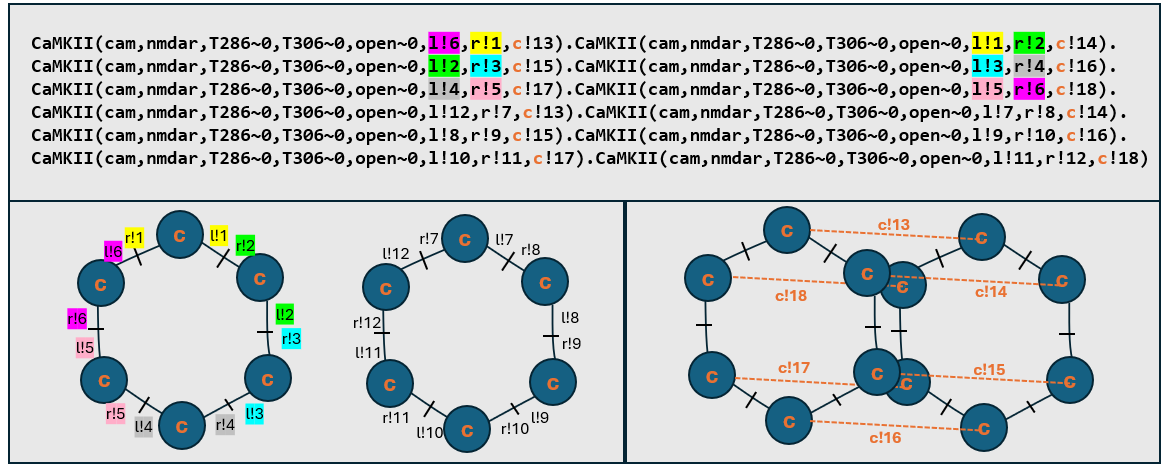
\includegraphics[width=0.95\linewidth,height=\textheight,keepaspectratio]{30-methods-figures/camkii_dodecamer_bngl.PNG}

}

\caption[CaMKII dodecamer in BNGL]{\label{fig-camkii-dodecamer}(A) The
open flag determines whether the subunit is in a closed (0) or open (1)
state. The T286 and T306 flags represent the phosphorylation states,
where a value of 0 indicates the subunit is unphosphorylated, and ``P''
indicates phosphorylation. The cam flag refers to a binding site for
CaM, which can either be bound or unbound. Similarly, the nmdar flag
represents another binding site for the NMDA receptor, which can also be
in a bound or unbound state. The cam and nmdar flags represent binding
events that can occur or not, depending on whether CaM or NMDA receptors
are bound to the subunit. (B) The left (l), right (r), and centre (c)
binding sites facilitate the assembly of subunits into two hexameric
rings. These rings are stabilised via interactions at the centre binding
site. Subunits participating in the left and right rings are highlighted
in matching colours to distinguish the respective assemblies. (C) A more
visual depiction of the two separated hexameric rings. (D) The centre
binding interactions are specifically highlighted to show the
dodecameric representation of CaMKII in the model.}

\end{figure}%

The model includes autonomous activation of CaMKII subunits, allowing
them to flicker between open and closed states when unbound to CaM and
unphosphorylated at T286 (see reaction rule \#5 in
Figure~\ref{fig-tbl-1}). The binding of CaM or phosphorylation at T286
stabilises the open state by preventing reversion to a closed
conformation. Additionally, CaM binding can only occur if the subunit is
in an open state due to the structural requirements for high-affinity
binding. Electron microscopy of rat \(\alpha\)-CaMKII in Sf9 cells
{[}\citeproc{ref-myers2017CaMKII}{164}{]} suggests that fewer than 3\%
of CaMKII subunits adopt a compact, docked-like conformation
{[}\citeproc{ref-bayer2019CaM}{449}{]}. The model therefore assumes all
CaMKII to be in an undocked confirmation, in order to streamline the
focus on the fundamental functional states of CaMKII.

Each CaMKII holoenzyme diffuses through the cell volume with a specified
diffusion constant of \(1\times 10^{-6} \text{cm}^2/\text{s}\), which is
within biological limits {[}\citeproc{ref-sanabria2008Spatial}{450}{]}.
In the model, CaMKII subunits can interact with NMDA receptors located
on the cell surface. When they interact, CaMKII can bind reversibly to
the NMDA receptor, forming a complex in which the CaMKII subunit that
has been bound remains open (see reaction rule \#12 in
Figure~\ref{fig-tbl-1}). As CaMKII remains open when bound to NMDARs,
further reactions can happen such as phosphorylation at T286 and T305,
as well as binding to CaM molecules (Figure~\ref{fig-camkii_nmdar} and
Figure~\ref{fig-camkii-binding-rxns}).

\subsection{CaMKII and NMDAR binding}\label{camkii-and-nmdar-binding}

In this model, NMDARs are represented as single-site molecules, rather
than as tetramers, due to the fact that the primary interaction between
CaMKII and NMDARs occurs predominantly through the GluN2B subunit. While
it is important to acknowledge that the GluN2B subunit is distinct from
the entire NMDAR heteromer, we refer to the model as NMDAR for
simplicity and clarity. This nomenclature is used as a practical
approximation, since the interactions we are modelling are specifically
associated with the GluN2B subunit, which is often studied in isolation
in experimental settings. In many in vitro experiments, the focus is on
the GluN2B subunit, and the behaviour of the whole NMDAR complex is
inferred based on these more controlled interactions
{[}\citeproc{ref-rumian2024LTP}{211},
\citeproc{ref-akashi2009NMDA}{216},
\citeproc{ref-goodell2014CaMKII}{451},
\citeproc{ref-barcomb2016CaMKIIa}{452}{]}. Therefore, for the purposes
of this model, referring to the system as NMDAR aligns with the
established experimental approach, even though the underlying
interactions are predominantly occurring via the GluN2B subunit. Further
developments of this model to account for a more complex NMDAR molecule
are possible, as I propose in Chapter~\ref{sec-discussion}.

\begin{figure}[H]

\centering{

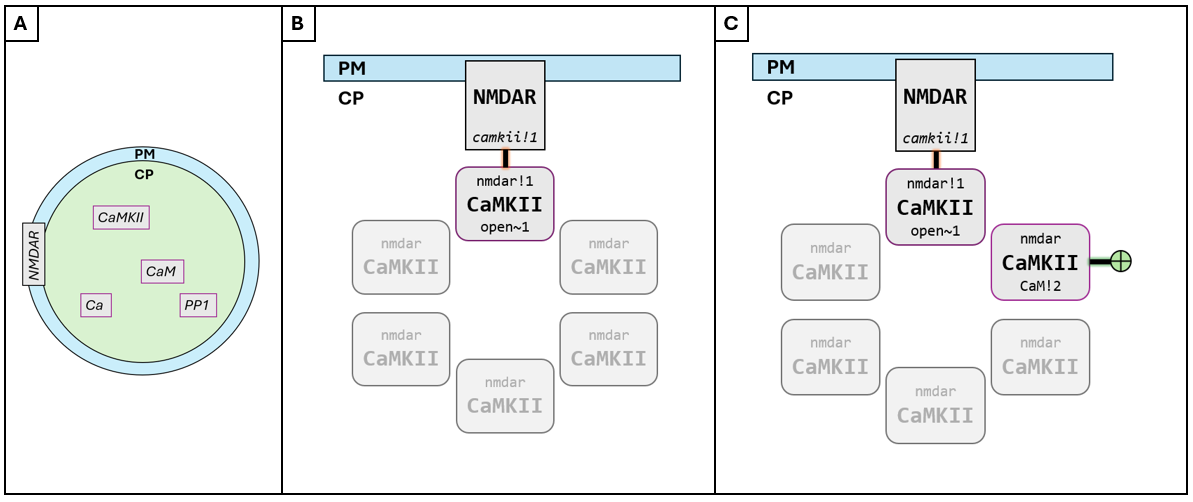
\includegraphics[width=0.85\linewidth,height=\textheight,keepaspectratio]{30-methods-figures/cbngl_camkii_nmdar.PNG}

}

\caption[Simplified schematic of CaMKII binding to NMDARs in
Compartmental BioNetGen]{\label{fig-camkii_nmdar}Simplified schematic of
CaMKII binding to NMDARs in Compartmental BioNetGen. (A) A cell is
defined with plasma membrane (PM) and cytoplasm (CP) volumes. Molecules
are released as surface molecules (NMDARs) or volume molecules (rest).
(B) NMDARs embedded in the PM can bind to CaMKII subunits diffusing
within the cytoplasm. (C) Different subunits within the CaMKII dodecamer
(simplified here as a hexamer) can independently interact with other
molecules such as NMDAR or CaM. These interactions can occur
simultaneously or asynchronously, allowing CaMKII to integrate multiple
signals through subunit-specific states.}

\end{figure}%

Furthermore, as previously discussed in
Section~\ref{sec-CaMKII-NMDAR-association}, the precise molecular
mechanism by which CaMKII binds to NMDARs is not yet fully understood.
Nonetheless, the literature seems to agree that CaMKII interaction with
the C-terminal domain (CTD) of NMDARs plays a key role in stabilising
CaMKII in its open, catalytically active conformation
{[}\citeproc{ref-bayer2001Interaction}{168},
\citeproc{ref-ozden2022CaMKIIb}{176},
\citeproc{ref-nicoll2023Synaptic}{203},
\citeproc{ref-bayer2006Transitionb}{214}{]}. In our model, CaMKII may
bind to an NMDAR provided that it is in the open conformation and that
the receptor possesses an available CaMKII-binding site (see reaction
rule 12 in Figure~\ref{fig-tbl-1}). Upon binding, a stable CaMKII/NMDAR
complex is formed, in which the kinase remains in its active state due
to the stabilisation of its open structure.

\subsection{Binding of calcium to calmodulin}\label{sec-binding-ca-cam}

CaM has four calcium-binding domains known as E-helix/F-helix hand
motifs (EFs), which are helix-loop-helix structures where calcium ions
can bind. These four EF hands are arranged into two structural lobes: an
N-terminal lobe containing two EF hands, and a C-terminal lobe
containing the other two EF hands. Each lobe can bind two calcium ions,
so in our model, CaM is capable of binding four calcium ions in total.
The N lobe binds calcium faster with lower affinity and the C lobe binds
slower with higher affinity
{[}\citeproc{ref-kawasaki2017Conformational}{453}{]}. Numerous models
have been developed to investigate the dynamics of calcium ions binding
to CaM {[}\citeproc{ref-stefan2008Allostericd}{432},
\citeproc{ref-pepke2010Dynamic}{454},
\citeproc{ref-gonzalez-andrade2016Insights}{455}{]}.
{[}\citeproc{ref-linkevicius2025Fitting}{456}{]} examined and compared
various of these models, providing a useful summary of the typical
categories for modeling CaM binding to \(\mathrm{Ca^{2+}}\). The model
used here falls under their proposed ``scheme 3''
(Figure~\ref{fig-scheme3-cam}), where calcium binds and unbinds to four
separate calcium binding sites in CaM. Unlike other models that
distinguish between CaM's N-terminal and C-terminal binding lobes, this
project does not, as the specifics of calcium binding to CaM are beyond
its scope and following ``scheme 3'' approach to calcium binding
produces biologically relevant results while avoiding complexity,
allowing us to focus on further CaMKII and NMDARs interactions.

\begin{figure}[H]

\centering{

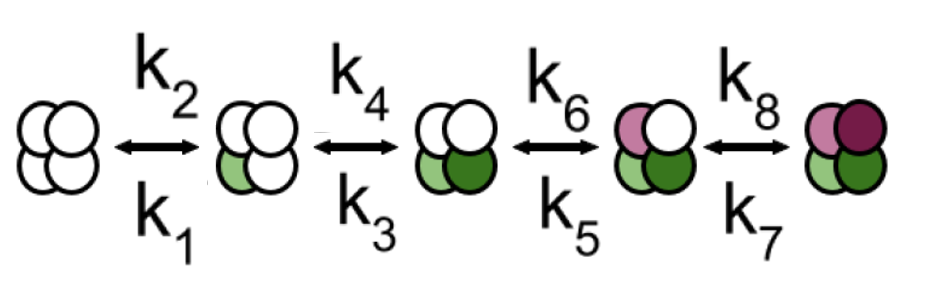
\includegraphics[width=0.7\linewidth,height=\textheight,keepaspectratio]{30-methods-figures/scheme3_cam.PNG}

}

\caption[Calcium binding to CaM]{\label{fig-scheme3-cam}We model calcium
binding to CaM following ``scheme 3'' proposed by Linkevicius et al.,
2024. It is a sequential CaM scheme where each binding site is
represented individually.}

\end{figure}%

\subsection{CaMKII subunits flicker between open and closed
states}\label{sec-camkii-flicker}

It is well established that CaMKII subunits can exist in both open and
closed conformations {[}\citeproc{ref-pullara2017Mechanisms}{457},
\citeproc{ref-zhang2017Opposing}{458}{]}, even in the absence of CaM
{[}\citeproc{ref-asciutto2021Physicalc}{459}{]}. While the notion that
CaM induces a conformational change in CaMKII is the common view, the
assumption that this binding event directly triggers subunit activation
is largely based on the induced-fit model, as discussed in
Section~\ref{sec-cam-binding-and-t286-p}. These observations may be due
to the fact that binding of \(\mathrm{Ca^{2+}}\)/CaM to CaMKII is more
likely when the CaMKII kinase subunits are in the open conformation.

CaMKII subunits inherently fluctuate between different conformational
states (open and closed), and an alternative perspective is that CaM
does not directly induce the opening of the subunit but rather
stabilises the open conformation upon binding
{[}\citeproc{ref-asciutto2021Physicalc}{459}{]}. This suggests that the
enzyme does not strictly require CaM to transition into an open state;
rather, CaM serves to stabilise and prolong this conformation, thereby
sustaining enzymatic activity. From a dynamic standpoint, it is
plausible that, in the absence of CaM, there exists a low probability of
the subunit adopting an open conformation due to intrinsic structural
fluctuations. Upon CaM binding, this equilibrium may shift, favouring
the stabilisation of the open state and ultimately leading to the full
activation observed in vitro
{[}\citeproc{ref-asciutto2021Physicalc}{459}{]}. Accordingly, in this
model, CaMKII subunits are considered to undergo spontaneous transitions
between open and closed conformations (see \#a in
Figure~\ref{fig-camkii-binding-rxns} for schematic depiction), and the
impact of CaM binding is assessed in terms of its stabilising effects on
these states.

CaM binding is not the only mechanism that can render CaMKII subunits in
their open conformation. In the model used in this PhD, as per the known
literature, CaMKII subunits can remain in an open conformation due to
one or more of the following events:

\begin{itemize}
\tightlist
\item
  CaM binding: CaM binding has been shown to structurally stabilise the
  open conformation of the CaMKII kinase subunit, preventing the kinase
  domain from re-engaging with its own regulatory region, thereby
  maintaining the open state
  {[}\citeproc{ref-hoffman2011Conformational}{171},
  \citeproc{ref-singla2001Molecular}{178},
  \citeproc{ref-gaertner2004Comparative}{179}{]}.
\item
  T286 phosphorylation: Phosphorylation at this site occurs at the hinge
  region of CaMKII and prevents subunits from closing
  {[}\citeproc{ref-chang2017CaMKII}{153},
  \citeproc{ref-braun1995Multifunctional}{186}--\citeproc{ref-buard2010CaMKII}{189}{]}.
  This modification thus sustains the subunit in an open conformation,
  contributing to the prolonged activation of the kinase.
\item
  NMDAR binding: Once a CaMKII subunit binds to the NMDA receptor, the
  interaction can stabilise the open state of the kinase. This
  CaMKII/NMDAR association has been shown to maintain the kinase in an
  active, open conformation, as discussed in
  Section~\ref{sec-CaMKII-NMDAR-association}.
\end{itemize}

\subsection{Binding of CaM to CaMKII}\label{sec-binding-cam-camkii}

CaM bound to different amounts of calcium has been shown to bind to
CaMKII with different affinities, with CaM bound to four calcium having
the highest affinity {[}\citeproc{ref-ordyan2020Interactions}{435},
\citeproc{ref-linkevicius2025Fitting}{456},
\citeproc{ref-khan2024Realtimea}{460}{]}. While CaM binding to the
low-affinity site is compatible with CaMKII remaining in a closed state,
binding to the high-affinity site is thought to structurally prevent
CaMKII from closing {[}\citeproc{ref-hoffman2011Conformational}{171},
\citeproc{ref-singla2001Molecular}{178},
\citeproc{ref-gaertner2004Comparative}{179}{]}. The literature suggests
that CaM binding in itself is not sufficient for CaMKII activation,
although high-affinity binding of CaM is
{[}\citeproc{ref-evans2009Energetics}{461}--\citeproc{ref-bossuyt2013Visualizing}{463}{]}.
This is likely due to the stabilising effect of high affinity binding of
CaM to CaMKII structurally keeping the kinase in its active state.

In this model, for simplicity, we therefore assume that only fully
saturated CaM with four calcium ions (CaM\_Ca4) binds to open CaMKII
subunits. Additionally, CaM binds to a CaMKII subunit only if T306 is
dephosphorylated. The T305/T306 site lies within the CaM binding region.
It has been shown that autophosphorylation at T305/T306 (T306 hereforth)
impedes CaM binding, and similarly CaM binding prevents T306
phosphorylation {[}\citeproc{ref-rellos2010Structure}{464}{]}. In the
model here, CaM is able to bind to CaMKII with the following rules:

\begin{itemize}
\tightlist
\item
  CaM must be fully saturated (bound to four calcium ions), i.e.~only
  CaM\_Ca4 binds to CaMKII. We assume only one high affinity binding
  site for CaM in each CaMKII subunit.
\item
  CaMKII subunit must be in its open/active state.
\item
  T306 must be unphosphorylated.
\end{itemize}

As described above in Section~\ref{sec-camkii-flicker} when a CaMKII
subunit spontaneously flickers into its active/open state CaM binding is
likely to stabilize the subunit once it is already active, but does not
initiate activation. Similarly, while it is commonly suggested that
simultaneous binding of CaM to two neighbouring subunits triggers T286
autophosphorylation, we propose that CaM's role might be more nuanced.
Instead of being essential for T286 phosphorylation, CaM may stabilize
the open state of CaMKII, thereby increasing the likelihood of
phosphorylation. Therefore, in this model, we do not make it a
requirement for CaM to be bound to neighbouring subunits for
phosphorylation to happen. We consider CaM binding is not strictly
necessary for autophosphorylation but rather enhances the probability of
phosphorylation by maintaining subunits in their active/open state.

\subsection{CaMKII phosphorylation and
dephosphorylation}\label{camkii-phosphorylation-and-dephosphorylation}

The most studied phosphorylation sites on CaMKII are T286 and T305/T306.
These sites are key for regulating CaMKII activity and subcellular
localization at the PSD during LTP, which is of relevance for synaptic
plasticity as well as learning and memory
see~\ref{sec-cam-binding-and-t286-p}. Likewise, in this study, we focus
on these two sites. While other phosphorylation sites on CaMKII have
been identified {[}\citeproc{ref-migues2006Phosphorylation}{465},
\citeproc{ref-gangopadhyay2008Regulation}{466}{]}, their functions are
not yet fully understood and are not within the scope of this study.

\subsection{T286 phosphorylation}\label{t286-phosphorylation}

I have modelled phosphorylation of T286 to occur with the condition that
two adjascent CaMKII subunits are in their open states. Research shows
that CaMKII subunits need to be open to expose the ATP binding site in
the regulatory domain, allowing the gamma-phosphate of ATP to transfer
to the threonine residue at T286
{[}\citeproc{ref-lou1986Activation}{467},
\citeproc{ref-hoffman2011Investigation}{468}{]}. The open (kinase domain
available) and undocked (subunits can reach their neighbours) states of
two neighbouring subunits is crucial for the catalytic site of one
subunit to reach and phosphorylate its neighbouring subunit. In our
model, we assume ATP molecule levels are sufficient to ensure the
reaction proceeds at its maximal rate (saturating), so we do not model
ATP as a reactant but rather focus on the phosphorylation process under
these conditions.

As discussed earlier, CaM bound to two neighbouring subunits is often
referred to in the literature as being required for autophosphorylation
and subsequent CaMKII activation
{[}\citeproc{ref-rellos2010Structureb}{180},
\citeproc{ref-nicoll2005Synaptic}{193}{]}. CaM has been shown to keep
CaMKII subunits in their open state, and therefore it may indirectly
enhance probability of T286 phosphorylation.

In the model I use here I don't make CaM a requirement for T286
phosphorylation, but rather once CaMKII is bound to CaM\_Ca4, this
binding keeps CaMKII subunits in their open state and further enables
phosphorylation. The only requirement for CaMKII T286 phosphorylation
is, therefore, that two adjacent subunits are in their open state to
enable inter subunit phosphorylation at this site (as per
Figure~\ref{fig-docked-undocked} previously described in
Chapter~\ref{sec-biology-chapter} and below in
Figure~\ref{fig-camkii-binding-rxns}).

\subsection{T306 phosphorylation}\label{t306-phosphorylation}

In contrast to T286 phosphorylation, T306 phosphorylation prevents
binding of CaM, as the phosphate group added to the threonine creates
electrostatic and steric interference, occupying the position where CaM
normally interacts. In the model used here, CaM can therefore only bind
to CaMKII if the T306 site is not phosphorylated, and conversely,
phosphorylation at T306 cannot occur while CaM is bound (previously
discussed in Section~\ref{sec-camkii-as-dodecamer}). Similar to the
conditions for T286, the model requires that a subunit must be in the
open state for phosphorylation at T306 to take place. Since T286
phosphorylation maintains subunits in their open state, phosphorylation
at T306 is more likely to occur if a neighbouring subunit is
phosphorylated at T286.

An aspect of phosphorylation at this site is that it does not prevent
CaMKII subunits from closing, unlike T286 phosphorylation
{[}\citeproc{ref-cook2021CaMKIIb}{198}{]}. This, together with the fact
that it prevents CaM from binding, makes it more likely that subunits
that are phosphorylated at T306 are found in the closed state too. When
the subunit is closed, catalytic activity of the kinase is reduced, as
the kinase domain is not accessible to perform catalytic activity.
Therefore, this phosphorylation is often referred to as reducing
catalytic activity of CaMKII. T306 phosphorylation may act as a form of
kinetic proofreading, by ensuring that CaMKII remains inactive, or less
active, unless sustained or repetitive calcium signals are present.
Phosphorylation at T306 likely prevents premature or excessive kinase
activity, thereby enhancing the specificity and fidelity of
CaMKII-mediated signalling in response to synaptic activity.

\subsection{Dephosphorylation of CaMKII
subunits}\label{dephosphorylation-of-camkii-subunits}

There are multiple known phosphatases which act to dephosphorylate
CaMKII in the PSD {[}\citeproc{ref-colbran2004Protein}{147},
\citeproc{ref-cohen1997Novel}{469}{]}. Different phosphatase proteins
will carry out their function depending on their localization and what
protein assemblies they are bound to or are available for them. The
Ser/Thr phosphatase PP1 is a key regulator of CaMKII signalling
{[}\citeproc{ref-shioda2017Physiological}{470}{]}; and it can
dephosphorylate both T286 and T306 sites of the kinase.

The colocalization with PSD-associated PP1 or sequestration away from
other protein phosphatases, such as protein phosphatase 2A or protein
phosphatase 2B (PP2A, PP2B), results in differential modulation of
CaMKII's T286 dephosphorylation. PP1 can form a complex with over 50
regulatory or scaffolding proteins that dictate substrate specificity
and subcellular localization. There are four known PP1 subunit isoforms
of the catalytic subunit (\(\alpha\), \(\beta\), \(\gamma\)-1, and
\(\gamma\)-2), each interacting with over 40 known regulatory and target
subunits. PP1-\(\alpha\) has been shown to account for the majority of
phosphatase activity with CaMKII in the PSD
{[}\citeproc{ref-colbran2004Protein}{147}{]}. Therefore, we focus on
PP1-\(\alpha\) in this study, and refer to it simply as PP1.

In the model used here, PP1 catalyzes the dephosphorylation of CaMKII
without forming a stable enzyme-substrate complex. Instead, the reaction
proceeds in a manner where PP1 transiently interacts, without binding,
with a CaMKII subunit under specific conditions, facilitating the
dephosphorylation process. PP1 can only dephosphorylate CaMKII subunits
when they are unbound from CaM, as CaM structurally obstructs access to
the T286 phosphorylation site. Additionally, the CaMKII subunit must be
in its open conformation to expose both the T286 and T306 sites for
PP1-mediated dephosphorylation.

\subsection{Reaction rules and kinetic
rates}\label{reaction-rules-and-kinetic-rates}

In BNGL, reaction rules are specified as discrete transformations. For
example, the rule ``CaM(ca\textasciitilde0,camkii) + Ca()
\textless-\textgreater{} CaM(ca\textasciitilde1,camkii)'' represents the
binding of a single calcium ion to CaM that is not bound to CaMKII (see
reaction \#1 in Figure~\ref{fig-tbl-1}). The assigned rate constants for
each rule are used to calculate the probability of the reaction
occurring when the two involved molecules collide, or at each time step
for unimolecular transformations.

As molecules diffuse within the simulation volume, all molecules within
a specified radius along a given trajectory or at the point of collision
on a surface are considered for potential reactions. For example, when a
calcium ion molecule encounters a free CaM molecule at the point of
collision, they react according to the specified rule in the model,
resulting in the formation of the molecule CaM\_Ca1. CaM\_Ca1 can
continue to diffuse based on the parameters defined in the simulation
and can interact with other molecules as well (see back for diagram
example explanation in Figure~\ref{fig-mcell-works}).

The reaction rules defined below follow the ``don't care, don't write''
principle of rule-based modelling: if a molecular feature is irrelevant
to a particular reaction, it is simply omitted from the reaction
definition. For example, in reaction \#5, which describes the flickering
of CaMKII subunits between open and closed states, the conditions
specified are that the subunit's CaM-binding site must be free, the
subunit must be unphosphorylated at T286, and the subunit must be open.
However, the phosphorylation state at T306 is irrelevant to this
reaction, and therefore is not specified.

\begin{figure}[H]

\centering{

\pandocbounded{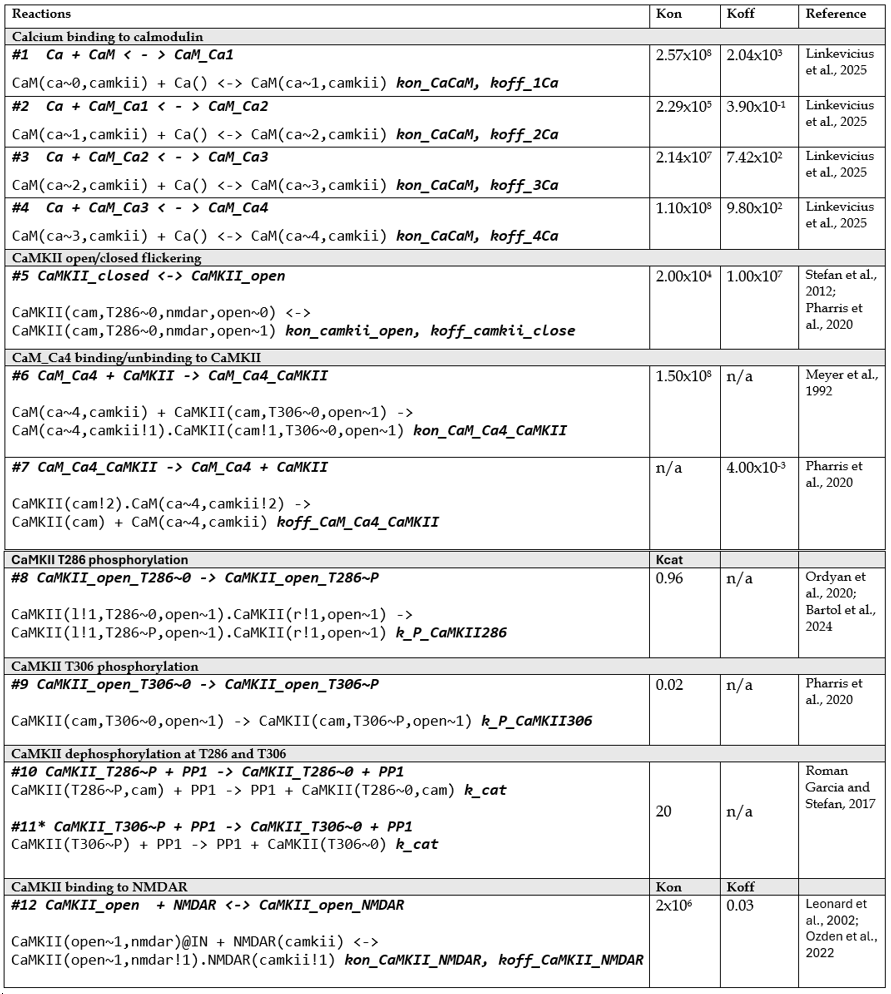
\includegraphics[keepaspectratio]{30-methods-figures/table_rxns1.PNG}}

}

\caption[Reactions and rate constants used in the
model]{\label{fig-tbl-1}Reaction rules and rate constants used in the
model. \(k_\text{on}\) (association rates) in M\(^{-1}\)s\(^{-1}\),
\(k_\text{off}\) (dissociation rates) in s\(^{-1}\), \(k_\text{cat}\)
(catalytic rates) in s\(^{-1}\).}

\end{figure}%

\begin{figure}[H]

\centering{

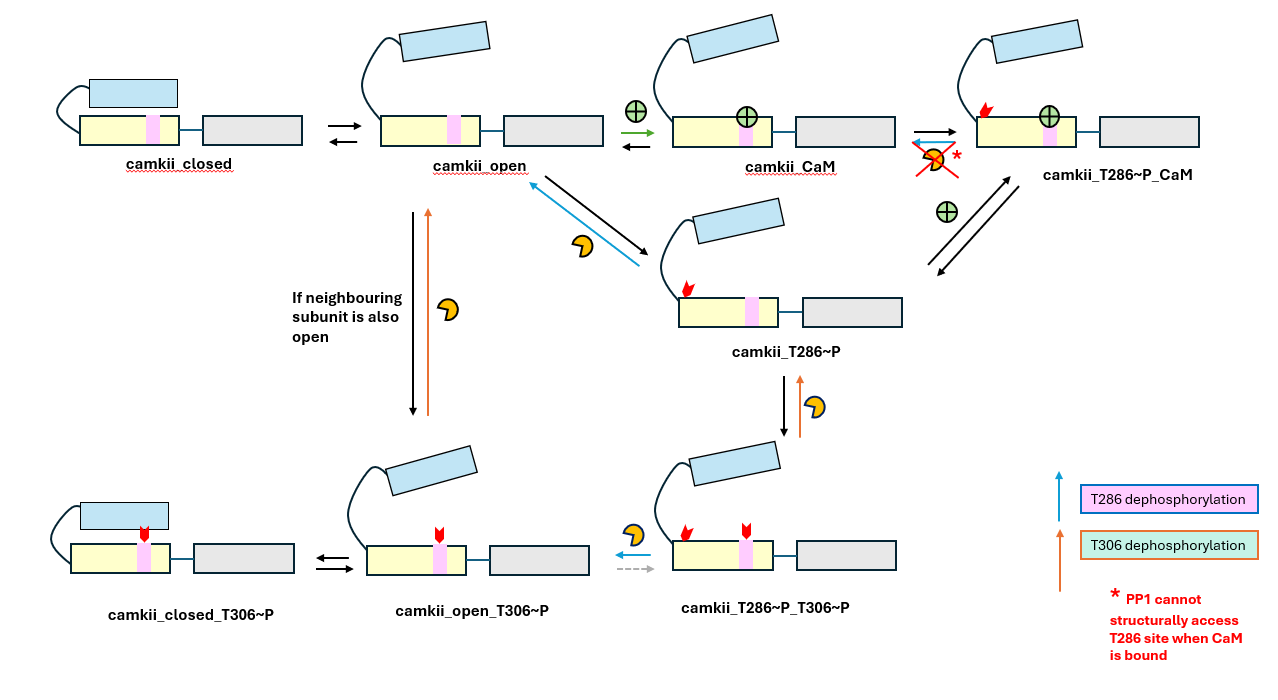
\includegraphics[width=0.9\linewidth,height=\textheight,keepaspectratio]{30-methods-figures/camkii-binding-rxns.PNG}

}

\caption[Reaction rules depicted for possible reaction pathways of
CaMKII subunits]{\label{fig-camkii-binding-rxns}Reaction rules depicted
for possible reaction pathways of CaMKII subunits. (\#a) CaMKII in a
closed state can flicker between open and closed states; (\#b) CaMKII
that is open can reversibly bind to a CaM molecule; (\#c) CaMKII that is
bound to CaM can phosphorylate at T286 (T286\textasciitilde P), and if
CaM is bound, PP1 cannot structurally access the subunit to
dephosphorylate it; (\#d) CaMKII that is open and free from CaM can also
phosphorylate at T286, and PP1 can access and dephosphorylate it in this
state; (\#e) CaMKII that is bound to CaM and T286\textasciitilde P can
release CaM and remain T286P; (\#f) CaMKII T286\textasciitilde P can
also phosphorylate at T306, and PP1 can dephosphorylate the T306 site as
well; (\#g) When CaMKII is phosphorylated at both sites, PP1 can also
dephosphorylate T286 instead of T306, and CaMKII that is T306P can also
autophosphorylate at T286; (\#h) CaMKII that is T306P can be
dephosphorylated by PP1, and if a CaMKII subunit that is open has a
neighbouring subunit that is also open, it may autophosphorylate at
T306; (\#i) CaMKII that is T306P can close (unlike when CaMKII is
T286\textasciitilde P).}

\end{figure}%

\section{Validating Model Behaviour}\label{sec-validating-model}

To validate the model, I focused on several key aspects: first, I
checked how closely the model matched biological reality and ensured it
was biologically plausible. I also built the model step by step,
allowing for gradual improvements and refinements. The kinetic
parameters for the model's reactions were either taken from existing
literature or estimated from experimental data. When there was
uncertainty, I ran parameter explorations to see how changes in the
kinetic rates affected the model's behaviour.

\subsection{Incremental Construction and Stepwise
Validation}\label{incremental-construction-and-stepwise-validation}

In order to validate model behaviour, each reaction rule was added one
at a time and tested to see if it produced biologically plausible
results. Reactions or sets of reactions were introduced sequentially and
tested independently. Structuring the model this way made it possible to
validate individual components before integrating them into the full
system. For example, the model was first tested by incorporating the
calcium binding to CaM reactions. These were validated by comparing the
outputs to those of a previously published and experimentally validated
model {[}\citeproc{ref-romangarcia2017Computationala}{471}{]}. Once
consistent behaviour was observed, the next layer ---CaM binding to
CaMKII--- was added and validated in a similar manner. Finally,
interactions between CaMKII and NMDARs were introduced and tested. While
a detailed account of each individual rule implementation is not
provided here for the sake of conciseness, a summary of the key reaction
layers and their expected outputs is presented in
Table~\ref{tbl-model-predictions}. Each row links an expected biological
behaviour to its underlying model rule(s), along with an indication of
whether the behaviour was observed in simulation results. These outputs
not only confirm that the system produces plausible results at each
stage but also serve as checkpoints for model development.

The list below presents a series of expected model behaviours that arise
from specific reaction rules defined in the model, as per
Figure~\ref{fig-tbl-1}.

\begin{longtable}[]{@{}
  >{\raggedright\arraybackslash}p{(\linewidth - 4\tabcolsep) * \real{0.6000}}
  >{\raggedright\arraybackslash}p{(\linewidth - 4\tabcolsep) * \real{0.2000}}
  >{\raggedright\arraybackslash}p{(\linewidth - 4\tabcolsep) * \real{0.2000}}@{}}
\caption{Summary of model predictions and expected
results.}\label{tbl-model-predictions}\tabularnewline
\toprule\noalign{}
\begin{minipage}[b]{\linewidth}\raggedright
Expected Result
\end{minipage} & \begin{minipage}[b]{\linewidth}\raggedright
Associated Reaction Rules
\end{minipage} & \begin{minipage}[b]{\linewidth}\raggedright
Observed in Models
\end{minipage} \\
\midrule\noalign{}
\endfirsthead
\toprule\noalign{}
\begin{minipage}[b]{\linewidth}\raggedright
Expected Result
\end{minipage} & \begin{minipage}[b]{\linewidth}\raggedright
Associated Reaction Rules
\end{minipage} & \begin{minipage}[b]{\linewidth}\raggedright
Observed in Models
\end{minipage} \\
\midrule\noalign{}
\endhead
\bottomrule\noalign{}
\endlastfoot
& & \\
\(\mathrm{Ca^{2+}}\) binds to CaM in a stepwise manner, with higher
affinity for forming CaM\_Ca3 and CaM\_Ca4 states. & Rules \#1 - \#4
(Figure~\ref{fig-tbl-1}) & No, see discussion. \\
& & \\
CaMKII autophosphorylation at T286 is increased by binding to NMDARs and
CaM. & Rules \#5, \#6, \#8, \#12 (Figure~\ref{fig-tbl-1}) & Yes, see
Figure~\ref{fig-camkii-t286p-nmdar-b} and 6.8 \\
& & \\
CaM binds CaMKII only in its fully saturated state (CaM\_Ca4),
stabilizing CaMKII in its open conformation. & Rule \#6
(Figure~\ref{fig-tbl-1}) & Yes, data not shown \\
& & \\
Open CaMKII binds to NMDARs, anchoring the kinase at the membrane . &
Rule \#12 (Figure~\ref{fig-tbl-1}) & Yes, see
Figure~\ref{fig-camkii-open} \\
& & \\
CaMKII undergoes autophosphorylation at T286 regardless of CaM binding,
though this phosphorylation is enhanced by CaM binding. & Rule \#8
(Figure~\ref{fig-tbl-1}) & Yes, see
Figure~\ref{fig-subsets-of-camkii-t286p-cam-binding} \\
& & \\
CaMKII is likely to undergo autophosphorylation at T306 following T286
phosphorylation, but T286 phosphorylation is not strictly required for
T306 phosphorylation to occur. & Rules \#8, \#9 (Figure~\ref{fig-tbl-1})
& Yes, see Figure~\ref{fig-t306p} and Figure~\ref{fig-t306p_anova} \\
& & \\
CaMKII subunits can be found to be T306-phosphorylated and in a closed
conformation. & Rules \#5, \#10 (Figure~\ref{fig-tbl-1}) & Yes, data not
shown. \\
\end{longtable}

\subsection{Sanity Checks}\label{sanity-checks}

As part of the model validation process, a series of sanity checks were
implemented to ensure the system behaved in accordance with known
biochemical rules and structural constraints. These checks primarily
aimed to verify that the model did not produce molecular species that
are biologically implausible or explicitly forbidden by the reaction
rules defined in the system.

Sanity checks were performed by recording observables in the BNGL model
file. These observables are explicitly commented with justifications
within the code itself and are structured to align with the logic and
reaction rules outlined in Figure~\ref{fig-tbl-1}. The purpose of these
observables is to serve as logical safeguards: if any of them yield a
nonzero value during simulation, it indicates a breach of the model's
core assumptions or rule constraints.

All sanity check observables listed below were expected to yield zero
values, and did so consistently in simulation results. This confirms
that the implemented reaction rules correctly prohibit the formation of
biologically impossible species. These results are consistent and
replicable; if the model is executed under the same rules and initial
conditions, these observables are expected to remain zero in any future
runs.

Below is a list of observables defined for sanity checks, along with a
description of the corresponding molecular species, and an explanation
of why their expected output should be zero under biologically valid
conditions.

\paragraph{\texorpdfstring{\textbf{CaMKII\_CaM\_Ca4\_PP}}{CaMKII\_CaM\_Ca4\_PP}}\label{camkii_cam_ca4_pp}

\begin{itemize}
\tightlist
\item
  Description: CaMKII bound to CaM (saturated with four Ca²⁺ ions),
  phosphorylated at both T286 and T306.
\item
  Expected Output: 0
\item
  Rationale: CaM binding and T306 phosphorylation are mutually
  exclusive. T306 lies within the CaM-binding domain of CaMKII, and its
  phosphorylation prevents CaM association. Thus, the coexistence of CaM
  and T306 phosphorylation is structurally impossible.
\end{itemize}

\paragraph{\texorpdfstring{\textbf{CaMKII\_CaM\_Ca4\_T306P1}}{CaMKII\_CaM\_Ca4\_T306P1}}\label{camkii_cam_ca4_t306p1}

\begin{itemize}
\tightlist
\item
  Description: CaMKII bound to CaM\_Ca4 phosphorylated at T306 only.
\item
  Expected Output: 0
\item
  Rationale: Similar to the case above, T306 phosphorylation sterically
  blocks CaM binding. Therefore, this species cannot exist under correct
  model logic.
\end{itemize}

\paragraph{\texorpdfstring{\textbf{CaMKII\_CaM\_closed}}{CaMKII\_CaM\_closed}}\label{camkii_cam_closed}

\begin{itemize}
\tightlist
\item
  Description: CaMKII bound to CaM\_Ca4 while in a closed conformation.
\item
  Expected Output: 0
\item
  Rationale: CaM binding induces a conformational opening of CaMKII.
  Thus, the closed state is incompatible with CaM-bound configurations.
\end{itemize}

\paragraph{\texorpdfstring{\textbf{CaMKII\_CaM\_unbound\_closed\_T286P1}}{CaMKII\_CaM\_unbound\_closed\_T286P1}}\label{camkii_cam_unbound_closed_t286p1}

\begin{itemize}
\tightlist
\item
  Description: CaMKII phosphorylated at T286, unbound to CaM, and in a
  closed state.
\item
  Expected Output: 0
\item
  Rationale: Phosphorylation at T286 stabilizes the open conformation of
  CaMKII. Once phosphorylated at T286, the subunit is expected to remain
  open and cannot revert to the closed conformation.
\end{itemize}

\paragraph{\texorpdfstring{\textbf{CaMKII\_closed\_complex}}{CaMKII\_closed\_complex}}\label{camkii_closed_complex}

\begin{itemize}
\tightlist
\item
  Description: CaMKII subunit is closed and bound to NMDAR forming
  NMDAR/CaMKII complex.
\item
  Expected Output: 0
\item
  Rationale: CaMKII can only bind to NMDARs if open and will remain open
  once bound, so none can be closed when bound in the NMDAR/CaMKII
  complex.
\end{itemize}

Beyond molecular states which were expected to yield a value of zero,
other sanity checks focused on conservation rules and population
consistency. For example, if a simulation starts with 100 CaMKII
subunits and 50\% are phosphorylated at T286, the remaining 50\% should
be in unphosphorylated. Any deviation from this expected balance may
indicate erroneous reaction pathways or state duplications. These sanity
checks were observed during simulation results and cross-validated with
the total molecule counts to ensure system integrity, as we will explore
in Chapter~\ref{sec-results}.

\subsection{Exploration of Uncertain
Parameters}\label{exploration-of-uncertain-parameters}

As discussed in Chapter~\ref{sec-intro-comp}, computational models can
serve as predictive tools to deepen our understanding of the mechanisms
underlying observed biochemical processes. However, parameters such as
rate constants, activation energies, diffusion coefficients, etcetera,
are rarely known with precision
{[}\citeproc{ref-sumathi2002Priori}{472}--\citeproc{ref-mcdonald2022Parameter}{474}{]}.
Consequently, predictions are typically subject to uncertainty. Thus
understanding how parameter variations influence outcomes is a crucial
part of model development and validation.

While other models have explored the dynamics of calcium, calmodulin,
and CaMKII {[}\citeproc{ref-pharris2019Multistate}{185},
\citeproc{ref-holmes2000Models}{427}--\citeproc{ref-bartol2024Spatial}{436}{]},
to the best of our knowledge none have specifically focused on the
direct interactions between CaMKII and NMDARs, as is done in the present
study. Consequently, determining parameters for calcium binding to CaM
and CaM binding to CaMKII was relatively straightforward, as there are
studies that have provided analyses and reviews of parameters that best
fit biological phenomena
{[}\citeproc{ref-linkevicius2025Fitting}{456}{]}. However, there were
four reaction parameters that were more uncertain and key for this
study: \(k_\text{on}\)/\(k_\text{off}\) for CaMKII flicker of opening
and closing (reaction rule \#5 in Figure~\ref{fig-tbl-1}), and
\(k_\text{on}\)/\(k_\text{off}\) for CaMKII binding to NMDARs (reaction
rule \#12 in Figure~\ref{fig-tbl-1}).

First, we examine the opening and closing kinetics of CaMKII subunits,
specifically focusing on the association \(k_\text{on}\) and
dissociation \(k_\text{off}\) rates of these two states. While most
models assume that CaM binding directly induces CaMKII activation, this
assumption is not applied in the current model, as discussed throughout
this thesis. Instead, we use the parameters proposed by
{[}\citeproc{ref-pharris2019Multistate}{185}{]}, as they modelled the
flickering (transient opening and closing) of CaMKII holoenzyme
subunits. However, since the current model integrates parameters from
multiple sources, parameter exploration was performed to ensure robust
and consistent dynamics aligned with the existing literature.
Specifically, we varied the opening and closing rates by factors of
0.01, 0.1, and 1 relative to the values proposed by Pharris et al.
{[}\citeproc{ref-pharris2019Multistate}{185}{]}, where \(k_\text{off}\)
= \(1.00 \times 10^7\) \(\mathrm{s}^{-1}\) and \(k_\text{off}\) =
\(2.00 \times 10^4\) \(\mathrm{M}^{-1}\mathrm{s}^{-1}\).

To ensure that the behaviour of CaMKII was well-understood and stable
before introducing additional complexity, I first modelled the changes
in the binding kinetics of CaMKII without the inclusion of NMDARs. This
approach allowed me to isolate and focus on the fundamental properties
of CaMKII itself. NMDARs introduce their own kinetic properties and
interactions with CaMKII, which could influence the system's behaviour.
By first confirming that CaMKII operates predictably in isolation, I
ensured that any subsequent changes observed after introducing NMDARs
could be confidently attributed to interactions between the two systems,
rather than unaccounted-for variations in CaMKII dynamics. By initially
focusing on CaMKII alone, I could verify that its kinetic behaviour was
stable and robust before layering on the complexities of NMDAR
interactions.

Figure~\ref{fig-open-close-t286p} and Figure~\ref{fig-open-close-camca4}
show the accumulation of CaMKII bound to CaM\_Ca4 and CaMKII T286
phosphorylation over time, under different kinetic conditions for the
opening and closing rates \(k_\text{on}\) and \(k_\text{off}\) of CaMKII
subunits. Each curve represents a simulation where \(k_\text{on}\) and
\(k_\text{off}\) were changed by factors of 0.01, 0.1, and 1 relative to
baseline parameters, while keeping the equilibrium dissociation constant
\(k_{\text{D}}\) fixed at 500\textasciitilde M. Even though
\(k_\text{on}\) and \(k_\text{off}\) differ across conditions (spanning
orders of magnitude), the general trajectory of molecule accumulation
over time remains broadly similar. Small differences are visible:
simulations with faster kinetics (higher \(k_\text{on}\) and
\(k_\text{off}\)) tend to show slightly faster initial accumulation, but
by the end (around 100 seconds), the molecule counts converge relatively
closely across all conditions.

Across both datasets, although \(k_\text{on}\) and \(k_\text{off}\) span
orders of magnitude, the general trajectory of molecule accumulation
remains broadly similar. Simulations with faster kinetics (higher
\(k_\text{on}\) and \(k_\text{off}\)) show a steeper initial
accumulation, reflecting more rapid binding and activation due to
quicker subunit opening and closing. However, by approximately 100
seconds, the total number of bound or phosphorylated molecules converges
across conditions.

Maintaining the same \(k_{\text{D}}\) isolates the effects of flickering
rates on early dynamics without confounding the overall binding
strength. Faster flickering enhances the speed at which steady-state is
approached, but does not alter the final outcome because the underlying
affinity remains the same. If \(k_{\text{D}}\) were instead varied, it
would affect not just the kinetics but also the steady-state occupancy,
leading to fundamentally different final amounts of CaMKII-CaM complexes
or T286-phosphorylated CaMKII.

These results led to the conclusion that varying \(k_\text{on}\) and
\(k_\text{off}\) by factors of 0.01, 0.1, and 1 did not significantly
affect the system's final outcomes. The system was robust enough that
these changes in flickering rates did not alter the overall behaviour,
making it reasonable to retain the original parameters proposed by
{[}\citeproc{ref-pharris2019Multistate}{185}{]}. Since altering the
rates did not drastically change the system's dynamics or steady-state
outcomes, the original parameter values were kept unchanged for the
final model simulations.

\begin{figure}[H]

\centering{

\pandocbounded{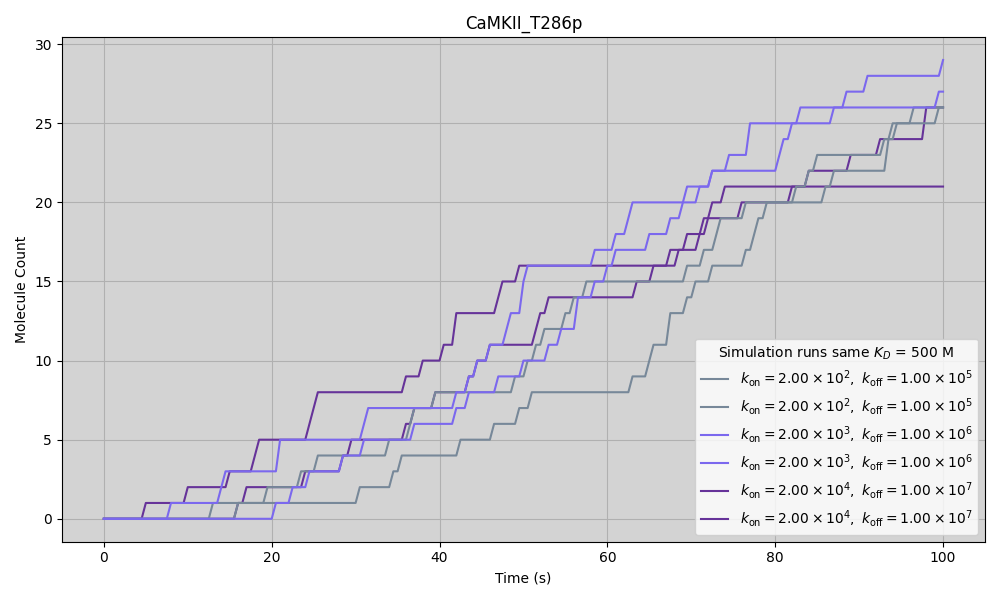
\includegraphics[keepaspectratio]{validation-figures/open-close-t286p.png}}

}

\caption[CaMKII T286 phosphorylation was unaffected by changes in
\(k_\text{on}\) and \(k_\text{off}\) for CaMKII opening parameter
sweep]{\label{fig-open-close-t286p}CaMKII T286 phosphorylation was
unaffected by changes in \(k_\text{on}\) and \(k_\text{off}\) by factors
of 0.1 and 0.01. The baseline values for \(k_\text{on}\) and
\(k_\text{off}\) were taken from
{[}\citeproc{ref-pharris2019Multistate}{185}{]}: \(k_\text{off}\) =
\(1.00 \times 10^7\) \(\mathrm{s}^{-1}\) and \(k_\text{off}\) =
\(2.00 \times 10^4\) \(\mathrm{M}^{-1}\mathrm{s}^{-1}\). Simulations
were performed by varying these parameters by factors of 0.1 and 0.01,
with the equilibrium dissociation constant (\(k_{\text{D}}\)) held
constant at 500 M.}

\end{figure}%

\begin{figure}[H]

\centering{

\pandocbounded{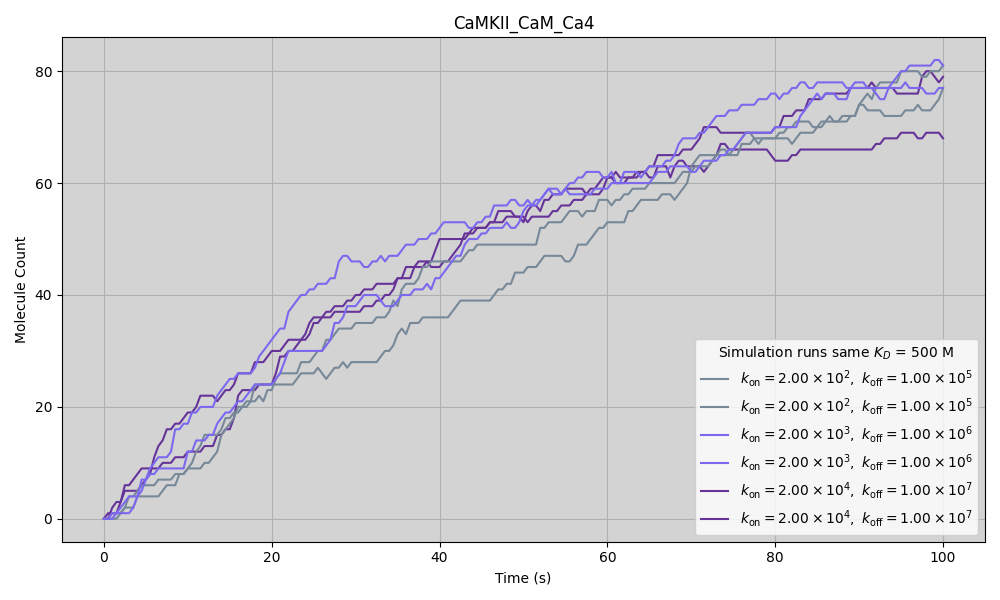
\includegraphics[keepaspectratio]{validation-figures/open-close-camca4.png}}

}

\caption[CaMKII binding to CaM was unaffected by changes in
\(k_\text{on}\) and \(k_\text{off}\) for CaMKII opening parameter
sweep]{\label{fig-open-close-camca4}CaMKII binding to CaM was unaffected
by changes in \(k_\text{on}\) and \(k_\text{off}\) by factors of 0.1 and
0.01. The baseline values for \(k_\text{on}\) and \(k_\text{off}\) were
taken from {[}\citeproc{ref-pharris2019Multistate}{185}{]}:
\(k_\text{off}\) = \(1.00 \times 10^7\) \(\mathrm{s}^{-1}\) and
\(k_\text{off}\) = \(2.00 \times 10^4\)
\(\mathrm{M}^{-1}\mathrm{s}^{-1}\). Simulations were performed by
varying these parameters by factors of 0.1 and 0.01, with the
equilibrium dissociation constant (\(k_{\text{D}}\)) held constant at
500 M.}

\end{figure}%

The objective was to determine how changes in these parameters affected
the molecules in the model. Specifically, we focused on CaMKII T286
phosphorylation and CaM binding, as they had been used in previous
parameter sweeps and were indirectly influenced by these changes. While
direct changes such as CaMKII binding or unbinding would obviously be
affected by the change in parameters that directly affect their
dynamics, T286 phosphorylation and CaM binding are not directly impacted
in the same way, making them suitable for testing the effects of
parameter variation on the system.

After varying \(k_{\text{D}}\) as described
(Figure~\ref{fig-nmdar-varying-kd-cam-ca4} and
Figure~\ref{fig-nmdar-varying-kd-camkiit286p}), we found a recent paper
proposing a \(k_{\text{D}}\) value of \(1.07 \times 10^{-7} \text{M}\).
Observing that the results did not vary significantly with this new
\(k_{\text{D}}\) value, which was in close agreement with our original
one, we proceeded with the choice of
\(k_{\text{D}} = 1.5 \times 10^{-7} \text{M}\).

Similarly, parameter variations for CaMKII and NMDAR binding rates were
explored to assess their impact on the model. Specifically, a
\(k_\text{off}\) for the unbinding of CaMKII from the NR1 subunit of
NMDARs was estimated by {[}\citeproc{ref-leonard2002Regulation}{125}{]}.
However, to the best of our knowledge, we could not find estimated
values for the GluN2B subunit, to which CaMKII binds more readily
{[}\citeproc{ref-strack1998Autophosphorylationdependent}{124}--\citeproc{ref-barria2005NMDA}{126}{]}.
We therefore proceeded to use the parameters from a previously validated
model {[}\citeproc{ref-romangarcia2017Computationala}{471}{]}, with a
\(k_{\text{D}}\) value of \(1.5 \times 10^{-7} \text{M}\). We ran the
simulation by varying this \(k_{\text{D}}\) by factors of 0.1 and 0.01.

\begin{figure}[H]

\centering{

\pandocbounded{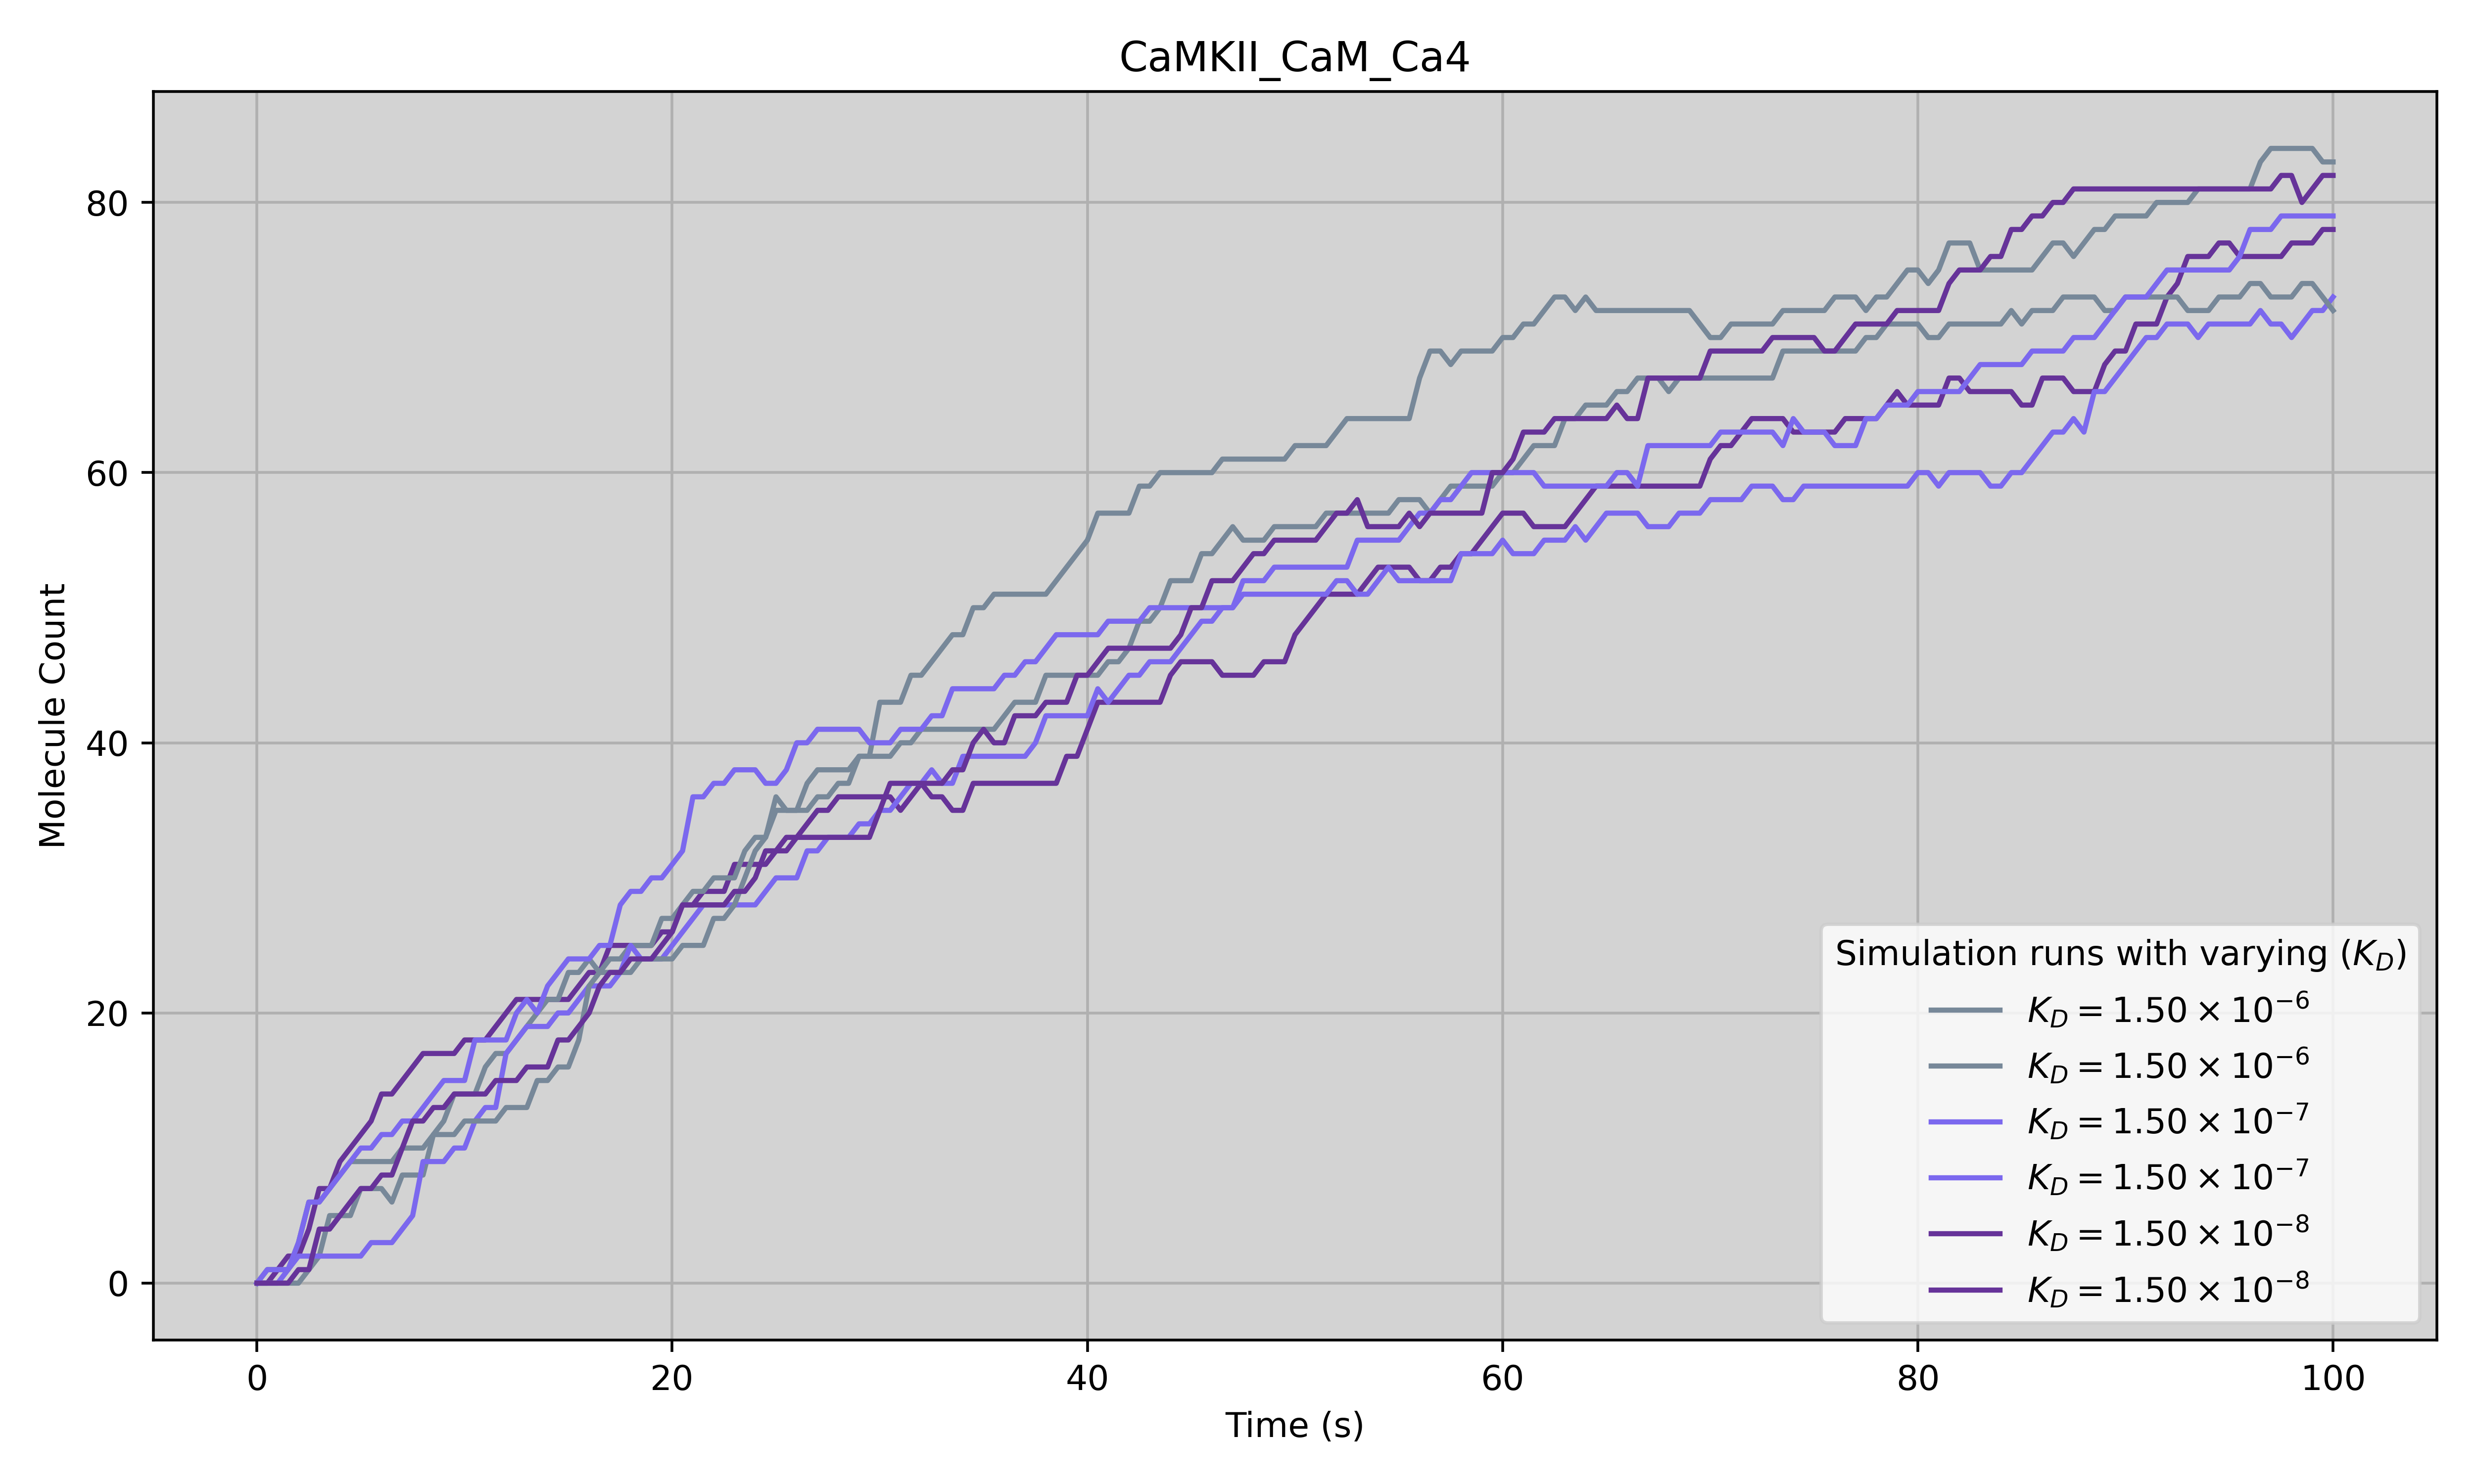
\includegraphics[keepaspectratio]{validation-figures/nmdar-varying-kd-cam-ca4.png}}

}

\caption[CaMKII T286 phosphorylation was unaffected by changes in
\(k_\text{on}\) and
\(k_\text{off}\)]{\label{fig-nmdar-varying-kd-cam-ca4}CaMKII binding to
CaM was unaffected by changes in \(k_{\text{D}}\) by factors of 0.1 and
0.01, from a previously used \(k_{\text{D}}\) value of
\(1.5 \times 10^{-7} \text{M}\)}

\end{figure}%

\begin{figure}[H]

\centering{

\pandocbounded{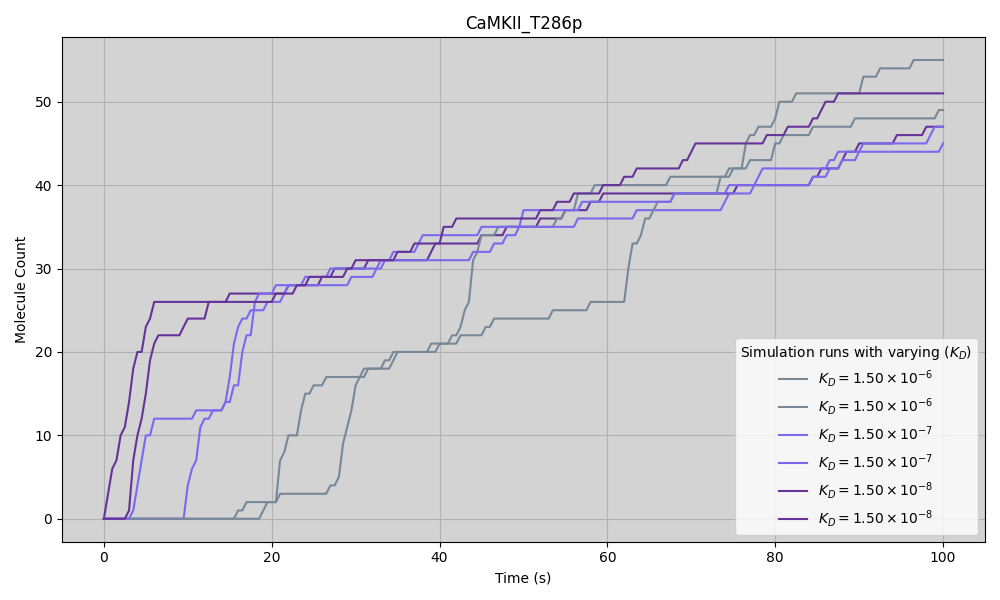
\includegraphics[keepaspectratio]{validation-figures/nmdar-varying-kd-camkiit286p.png}}

}

\caption[CaMKII binding to CaM was unaffected by changes in
\(k_\text{on}\) and
\(k_\text{off}\)]{\label{fig-nmdar-varying-kd-camkiit286p}CaMKII T286
phosphorylation CaMKII binding to CaM was unaffected by changes in
\(k_{\text{D}}\) by factors of 0.1 and 0.01, from a previously used
\(k_{\text{D}}\) value of \(1.5 \times 10^{-7} \text{M}\)}

\end{figure}%

Taken together, these parameter sweeps demonstrate that the model's core
behaviours, particularly CaMKII T286 phosphorylation and CaM binding,
are robust to substantial variations in both flickering kinetics and
CaMKII--NMDAR binding affinities. Despite exploring parameter changes
across multiple orders of magnitude, the system consistently converged
on similar outcomes. Based on this robustness, and the agreement with
literature-based estimates, the final parameters selected were the
original literature-based parameters.

\section{Expected Model Outcomes}\label{sec-expected-outputs}

In addition to direct rule-by-rule validation and sanity checks, I
defined a set of expected outcomes to assess whether the model could
produce emergent behaviours consistent with known biological
expectations---despite these behaviours not being explicitly hardcoded.
These behaviours arise not from isolated reactions, but from the
interaction and timing of multiple rules within the network, offering
important insight into whether the system captures the complex,
context-dependent behaviour observed in vivo.

For instance, phenomena such as the sustained opening of CaMKII
following transient calcium signalling are not encoded as fixed
outcomes. Instead, they should emerge from the model structure if the
underlying mechanisms of encoded rules are implemented correctly.
Similarly, the transition from CaM-dependent to CaM-independent
anchoring at NMDARs, are emergent outcomes expected to arise from the
model's rule interactions. The following emergent behaviours were not
coded into the rules in Figure~\ref{fig-tbl-1}, but were expected
behaviours to follow what is known in the literature.

\begin{enumerate}
\def\labelenumi{\arabic{enumi}.}
\item
  \textbf{CaMKII phosphorylation at T286 occurs regardless of CaM
  binding, although phosphorylation is more likely when CaM is present.}
  This behaviour is not explicitly hardcoded into the model, but is
  expected as an emergent property of the system. Both CaM binding and
  T286 phosphorylation stabilise the CaMKII subunit in its open
  conformation (rules \#6 and \#8), which increases the likelihood of
  both events co-occurring. Therefore, while the model does not directly
  specify this co-occurrence, the chances of T286 phosphorylation are
  indirectly increased when CaMKII is either already phosphorylated at
  T286 or bound to CaM, as both conditions promote an open state
  conducive to phosphorylation.
\item
  \textbf{When phosphorylated at T286, CaMKII binds more readily to
  NMDARs, independent of the presence of CaM.} This behaviour arises
  from the fact that T286 phosphorylation stabilises CaMKII in its open
  conformation, and only open CaMKII can bind to NMDARs. While the model
  does not explicitly encode a direct link between T286 phosphorylation
  and NMDAR binding, it encodes the conditions that promote each event
  separately. As a result, we expect that T286-phosphorylated CaMKII
  subunits will indirectly bind NMDARs more readily due to their
  maintained open state.
\item
  \textbf{When CaMKII is maintained in the open state by CaM binding,
  the kinase binds more readily to NMDARs and is likely to remain
  associated with the NMDAR/CaMKII complex even after CaM dissociates.}
  Both CaM binding and NMDAR binding stabilise CaMKII in its open
  conformation. The model allows multiple routes to maintaining this
  open state, one of them being CaM binding, hence CaM-bound CaMKII may
  be more likely to interact with NMDARs, and once that interaction
  occurs, the open conformation can be preserved by NMDAR binding alone.
\end{enumerate}

These expected behaviours serve as key indicators of the model's
capacity to recapitulate biologically realistic dynamics through rule
interactions alone. How these behaviours emerge in simulation is
examined in detail in Chapter~\ref{sec-discussion}, where the model's
outputs are evaluated against known experimental observations.

\bookmarksetup{startatroot}

\chapter{\texorpdfstring{Results of \emph{In Silico} Wild-Type and
Mutant
Models}{Results of In Silico Wild-Type and Mutant Models}}\label{sec-results}

Three principal model versions of the CaMKII/NMDAR model have been
developed. The first is a wild-type (WT) model, as described in
Chapter~\ref{sec-model-description}. In addition, two mutant (MT) models
were constructed: one in which CaMKII is unable to phosphorylate at
T286, and another in which CaMKII cannot bind to NMDARs. These mutations
were implemented by setting the reaction rates corresponding to CaMKII
autophosphorylation and CaMKII--NMDAR binding, respectively, to zero.

The simulations were designed to observe whether known emergent
behaviours of CaMKII could be reproduced by the model without being
explicitly encoded. In particular, following the expected outputs stated
in Section~\ref{sec-expected-outputs}, I looked for: (1) phosphorylation
at T286 occurring with or without CaM binding; (2) increased NMDAR
binding by T286-phosphorylated CaMKII; and (3) enhanced NMDAR binding in
the CaM-bound open state, with continued association after CaM
dissociation.

The results show that two out of the three expected behaviours emerge
from the model dynamics. T286 phosphorylation was more likely when CaM
was bound, though not strictly dependent on it. Similarly,
T286-phosphorylated CaMKII was increased through NMDAR binding due to
its stabilised open state. Finally, CaMKII bound to CaM binding and
NMDAR association were shown to be independent. These observations will
be discussed in more detail in the sections that follow.

\section{Analysis of the Wild-type
model}\label{analysis-of-the-wild-type-model}

This section presents a summary of the results obtained from the WT
model. In the WT simulation, the final total number of CaMKII\_open
molecules reaches a mean of approximately 108 molecules at 100 seconds.
The shaded area surrounding the mean trajectory in the graph represents
the standard deviation (SD), indicating the degree of variability across
different simulation runs.

\subsection{CaM binding and NMDAR binding independently stabilise CaMKII
activity in the early stages of the
simulation}\label{cam-binding-and-nmdar-binding-independently-stabilise-camkii-activity-in-the-early-stages-of-the-simulation}

Figure~\ref{fig-t286p-means} provides an overview of the key molecular
interactions and states observed in the WT CaMKII/NMDAR model during the
simulation. Each subpanel (a--d) captures specific aspects of the
molecular dynamics, focusing particularly on the interplay between
CaMKII opening, T286 phosphorylation, CaM binding, and NMDAR binding.

Panel (a) in Figure~\ref{fig-t286p-means} shows the evolution of the
open conformation of CaMKII over time. The brown line represents the
total number of CaMKII\_open subunits, which steadily increases as the
simulation progresses. Two main factors contribute to the stabilisation
of CaMKII in the open state: (1) CaM binding (light blue line,
camkii\_cam\_unbound\_open) and (2) NMDAR binding (dark blue line,
nmdar\_camkii\_complex). Notably, NMDAR binding can maintain CaMKII in
the open conformation even in the absence of CaM binding (Fig 7.2c).
Figure 7.2b focuses on T286 phosphorylation dynamics of CaMKII. The
orange line (camkii\_t286p) shows the total number of CaMKII subunits
phosphorylated at T286, while the pink line
(camkii\_t286p1\_bound\_nmdar) represents the subset of
T286-phosphorylated subunits that are also bound to NMDARs. A large
fraction of phosphorylated subunits are found associated with NMDARs,
indicating that NMDAR binding promotes or sustains T286 phosphorylation.
Importantly, this phosphorylation happens largely independently of CaM,
as further illustrated in panels (c) and (d).

Panel (c) in Figure~\ref{fig-t286p-means} dissects the
T286-phosphorylated CaMKII subunits that are bound to NMDARs into
CaM-bound and CaM-unbound populations. Here, the pink line represents
all T286-phosphorylated CaMKII subunits bound to NMDARs, while the
orange line shows the subset that are CaM-free
(camkii\_cam\_unbound\_t286p1\_bound\_nmdar). It is clear that the
majority of the T286-phosphorylated CaMKII subunits bound to NMDARs are
unbound from CaM, emphasizing that CaMKII can maintain phosphorylation
at T286 even after CaM dissociates. This further supports the idea that
NMDAR binding alone is sufficient to stabilize the active, open,
phosphorylated state in this model. Figure 7.2d provides a more detailed
look at T286 phosphorylation in relation to CaM binding across the whole
CaMKII population. The data shows that roughly equal numbers of CaMKII
subunits are phosphorylated at T286 whether they are CaM-bound or
CaM-unbound. This demonstrates that although CaM binding facilitates
CaMKII opening and activation, T286 phosphorylation does not require
continuous CaM binding once CaMKII is locked in its open, phosphorylated
conformation.

To further dissect the molecular events underlying these dynamics, the
following sections will explore a representative simulation run in
detail, focusing on the specific behaviours of CaMKII subunits in
relation to NMDAR and CaM binding, and T286 phosphorylation. For
reproducibility, the simulation run used for the single-run figures was
``run\_2025-04-03\_08-45-21\_seed\_2''. The model simulation files is
available in the model's GitHub repository page:
https://github.com/Susana465/CaMKII\_hexa\_bgnl\_to\_mcell. In order to
facilitate comprehensive understanding of the molecule names used, a
summary is provided in Figure~\ref{fig-observable_names}.

\begin{landscape}

\begin{figure}

\centering{

\pandocbounded{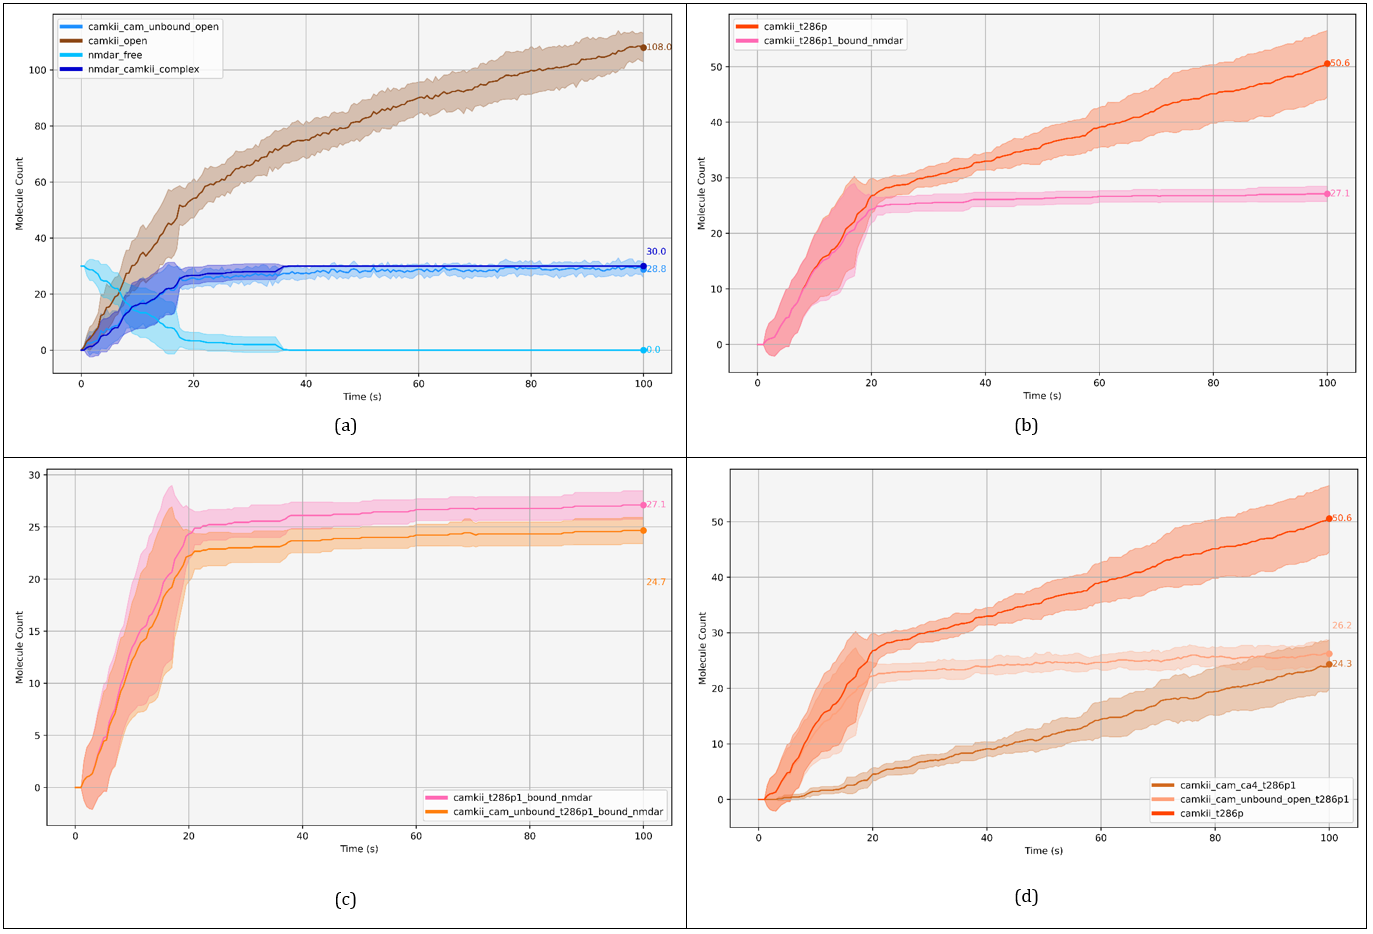
\includegraphics[keepaspectratio]{40-results-figures/WT/t286p-means.PNG}}

}

\caption[CaM binding and NMDAR binding independently stabilise CaMKII
activity]{\label{fig-t286p-means}CaM binding and NMDAR binding
independently stabilise CaMKII activity in the early stages of the
simulation. Final value means of total molecule counts (mean ± SD):
camkii\_open (108.00 ± 5.12); camkii\_cam\_ca4 (79.22 ± 3.85);
nmdar\_free (0.00 ± 0.00); nmdar\_camkii\_complex (30.00 ± 0.00);
camkii\_t286p (50.56 ± 5.96); camkii\_t286p1\_bound\_nmdar (27.11 ±
1.37); camkii\_cam\_unbound\_t286p1\_bound\_nmdar (24.67 ± 1.25);
camkii\_cam\_ca4\_t286p1 (24.33 ± 4.45);
camkii\_cam\_unbound\_open\_t286p1 (26.22 ± 2.35)}

\end{figure}%

\end{landscape}

\begin{figure}

\centering{

\pandocbounded{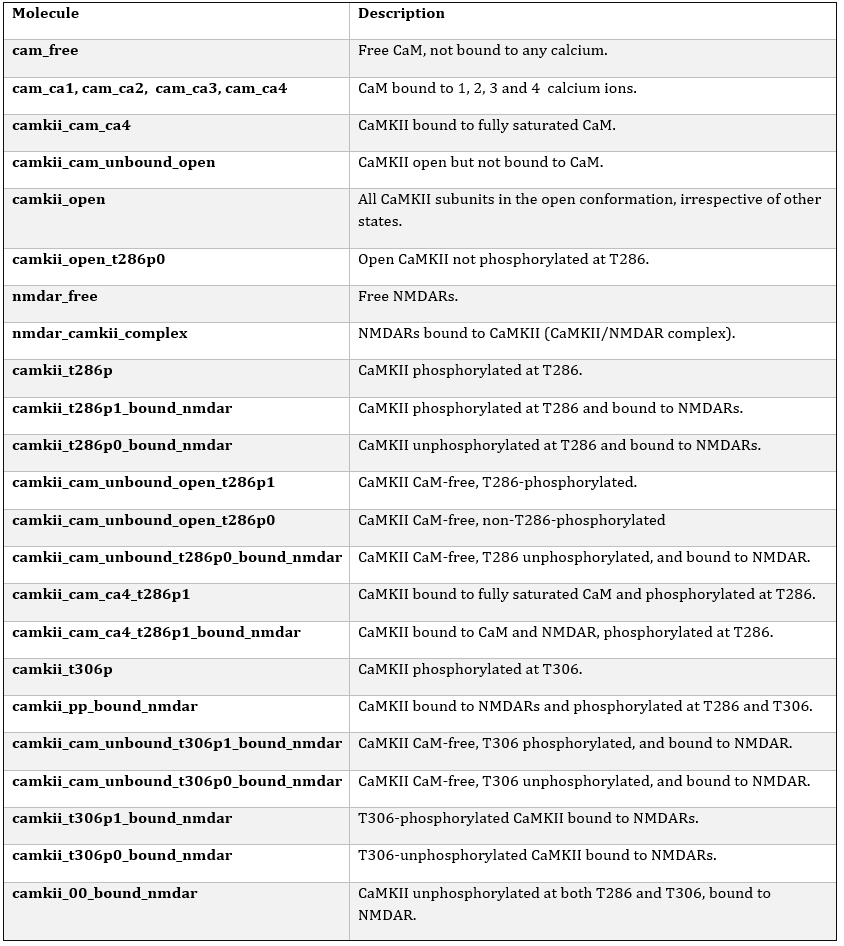
\includegraphics[keepaspectratio]{40-results-figures/observable_names.PNG}}

}

\caption{\label{fig-observable_names}Summary of observable names and
their meaning.}

\end{figure}%

\subsection{Approximately half of CaM binds to calcium within the first
5s}\label{approximately-half-of-cam-binds-to-calcium-within-the-first-5s}

In the WT model (described in detail in
Chapter~\ref{sec-model-description}), a release of 1000 calcium ions
occurs within a dendritic spine volume of 0.50588 \(\mu\text{m}^3\).
This calcium subsequently binds to CaM, which can bind up to four
calcium ions. Full saturation of CaM is required for subsequent binding
to CaMKII, resulting in the formation of the CaMKII--CaM complex
(CaMKII\_CaM\_Ca4).

This progression is illustrated in (Figure~\ref{fig-calcium-binding}),
where the gradual formation of partially and fully calcium-bound CaM
species is shown. Although calcium itself is not displayed (due to its
relatively high concentration distorting the plot scale), the stepwise
increase in CaM species bound to one, two, three, and four calcium ions
is clearly visible. The appearance of CaMKII bound to fully saturated
CaM (camkii\_cam\_ca4) further confirms the expected dynamics. as per
the set reaction rates and established literature, CaM fully bound to
four calcium ions is immediately available for binding to CaMKII,
whereas CaM bound to fewer calcium ions is less readily available for
this interaction.

The simulation reveals a rapid decrease in the concentration of free
CaM, which stabilises at approximately half of its initial value,
suggesting that roughly half of the CaM molecules remain unbound to
calcium. Upon further investigation, this suggests that calcium is
acting as a saturating factor. Given that each CaM molecule can bind up
to four calcium ions, the 290 CaM molecules would require at least 1200
calcium ions (290 × 4 \(\approx\) 1200) for full saturation. However,
the model uses 1000 calcium ions, which is slightly below this
threshold. It is also worth noting that calcium ions are continuously
binding to and dissociating from CaM as part of the ongoing reactions,
so as some calcium may dissociate from one species, it might then
associate to another, allowing for dynamic and emergent molecule
behaviours. Even if the calcium concentration were increased (the
difference between 1000 and 1200 calcium ions would be relatively small,
from 3.282 \(\mu\text{M}\) to 3.938 \(\mu\text{M}\), respectively), we
would expect an increase in the number of CaM molecules bound to four
calcium ions, but the change might not be substantial.

\begin{figure}[H]

\centering{

\pandocbounded{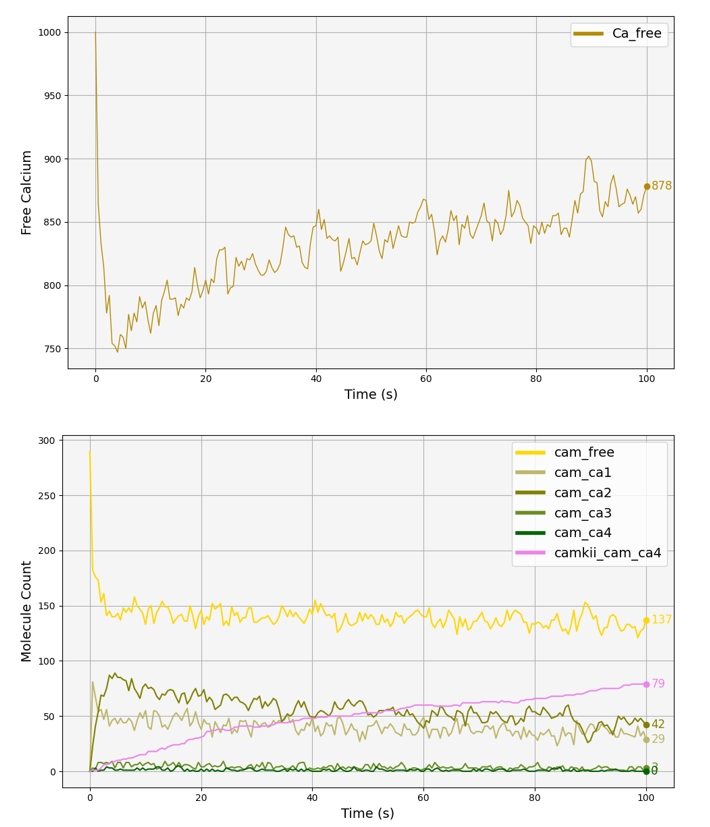
\includegraphics[keepaspectratio]{40-results-figures/WT/calcium-binding.png}}

}

\caption[CaM binding calcium]{\label{fig-calcium-binding}(Top) The
concentration of free calcium initially drops sharply as it binds to CaM
species, before stabilizing and gradually increasing toward the end of
the simulation. Shown separate to other molecules due to difference in
scale. (Bottom) The molecular counts of different CaM species show the
distribution of CaM bound to 1, 2, 3, and 4 calcium ions
(cam\_ca1--cam\_ca4), free CaM (cam\_free), and the CaMKII--CaM\_Ca4
complex. Free CaM rapidly decreases after the start, while CaM species
with bound calcium transiently rise. The CaMKII\_CaM\_Ca4 complex
steadily accumulates over time, indicating progressive activation of
CaMKII through CaM binding.}

\end{figure}%

\subsection{CaM stabilises CaMKII in the open conformation, but is not
required for CaMKII/NMDAR
binding}\label{cam-stabilises-camkii-in-the-open-conformation-but-is-not-required-for-camkiinmdar-binding}

Next, we examine CaM--CaMKII binding
(Figure~\ref{fig-cam-camkii-binding}), focusing on how CaMKII's open
conformation of subunits stabilises over time. Out of the 720 CaMKII
subunits released (not shown), a total of 104 molecules remain in the
open conformation (camkii\_open), at 100 seconds. Camkii\_open represent
the total population of CaMKII subunits that are structurally in their
open state. To determine how many of these open subunits are
simultaneously bound to CaM, we refer to the pink trace in
Figure~\ref{fig-cam-camkii-binding}, which indicates that 79 subunits
are CaM-bound by the end of the simulation. This shows that
approximately 75\% of the open CaMKII subunits are being stabilised in
this state through CaM binding up until the end of the simulation.

In contrast, the population of open CaMKII subunits that are not bound
to CaM reaches equilibrium just before the 20-second mark, maintaining a
steady count of just above 20 molecules until the end of the simulation.
This accounts for the remaining 25\% of the open CaMKII pool. These
observations indicate that the majority of open CaMKII subunits are
stabilised in their active conformation via CaM binding, while a smaller
proportion is maintained in the open state by alternative mechanisms.

In the model at hand, CaMKII is defined as dynamically transitioning
between open and closed conformations, and unless stabilised in the open
state ---either through CaM binding, T286 phosphorylation, or NMDAR
association--- it will revert to the closed state (see
Figure~\ref{fig-tbl-1}). So we can see in
Figure~\ref{fig-cam-camkii-binding} that the majority of CaMKII open is
stabilised by CaM, however, there is another mechanism that is keeping
CaMKII open. This other mechanism is in direct relation with NMDAR
interaction as we will explore next.

By examining Figure~\ref{fig-camkii-opening-nmdar}, we observe that the
levels of CaMKII binding to NMDARs (dark blue line:
nmdar\_camkii\_complex) closely follow the same pattern as CaM unbinding
from CaMKII (medium blue: camkii\_cam\_unbound\_open). In other words,
as CaMKII associates with NMDARs, this interaction maintains CaMKII in
an open state, without the need for CaM binding to CaMKII.

Interestingly, the proportion of CaMKII free from CaM that are still in
their open conformation (medium blue: camkii\_cam\_unbound\_open,
Figure~\ref{fig-camkii-opening-nmdar}) fluctuates up and down
frequently, which comes from CaMKII opening and closing (as CaM is not
bound yet).

Initially, the level of CaMKII free from CaM that are still in their
open conformation (camkii\_cam\_unbound\_open) fluctuates and exceeds
the amount of CaMKII bound to NMDARs (nmdar\_camkii\_complex). This
indicates that while a pool of open CaMKII is available, not all of it
is bound to NMDARs at once. Over time, as CaMKII binding to NMDARs
progresses and the system approaches a steady state, newly opened CaMKII
subunits are quickly captured by available NMDAR binding sites.
Consequently, the amount of free, open CaMKII stabilizes at a level
consistently lower than the amount of NMDAR-bound CaMKII, indicating
that binding to NMDARs efficiently sequesters and stabilizes open CaMKII
in the later phase.

Moreover, in Figure~\ref{fig-camkii-opening-nmdar}, we observe a
three-step, ladder-like progression of CaMKII binding to NMDARs. Each
step corresponds to an increase in the number of CaMKII subunits bound:
first reaching approximately 12 subunits, then 24, and finally 30. This
pattern suggests that entire CaMKII holoenzymes (each containing 12
subunits) sequentially bind to NMDARs. Here, looking at a single run
reveals a clear pattern that was obscured when averaging across multiple
simulations

Initially, one holoenzyme binds rapidly, with its subunits quickly
associating with available NMDARs. The process of a second holoenzyme
binding is slower, likely because after the first 12 subunits are bound,
there are fewer free NMDARs left. Now, the second holoenzyme has fewer
choices, and it may need to ``search'' or ``diffuse'' around more to
find free receptors. Finally, after the second holoenzyme binds (up to
24 subunits), a third holoenzyme binds partially, occupying the
remaining 6 NMDARs. By the time the third holoenzyme tries to bind, only
6 NMDARs are free --- not enough for all 12 subunits. The progressive
slowing reflects decreasing availability of free NMDARs for binding. The
implications of these findings are discussed in
Chapter~\ref{sec-discussion}. However, this particular mode of CaMKII
binding to NMDARs may be an artifact of the model. Although not
necessarily invalid, this aspect warrants further scrutiny and should be
revisited in future research, as explored further in the discussion
section below.

In summary, the majority (75\%) of CaMKII subunits in the open
conformation are stabilized by binding to CaM. However, while CaM helps
stabilize CaMKII in the open state, the binding of CaMKII to NMDARs is
not dependent on CaM. As CaMKII binds to NMDARs, it maintains its open
conformation even without CaM binding, indicating that the interaction
between CaMKII and NMDARs can stabilize the open state of CaMKII
independently of CaM.

\begin{figure}[H]

\begin{minipage}{\linewidth}

\centering{

\pandocbounded{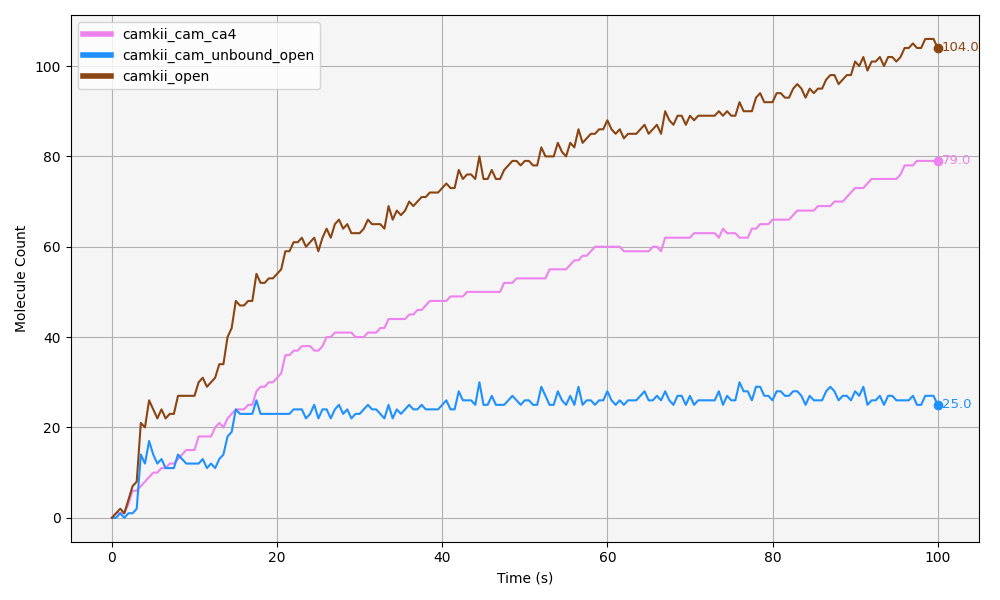
\includegraphics[keepaspectratio]{40-results-figures/WT/cam-camkii-binding.png}}

}

\subcaption{\label{fig-cam-camkii-binding}}

\end{minipage}%
\newline
\begin{minipage}{\linewidth}

\centering{

\pandocbounded{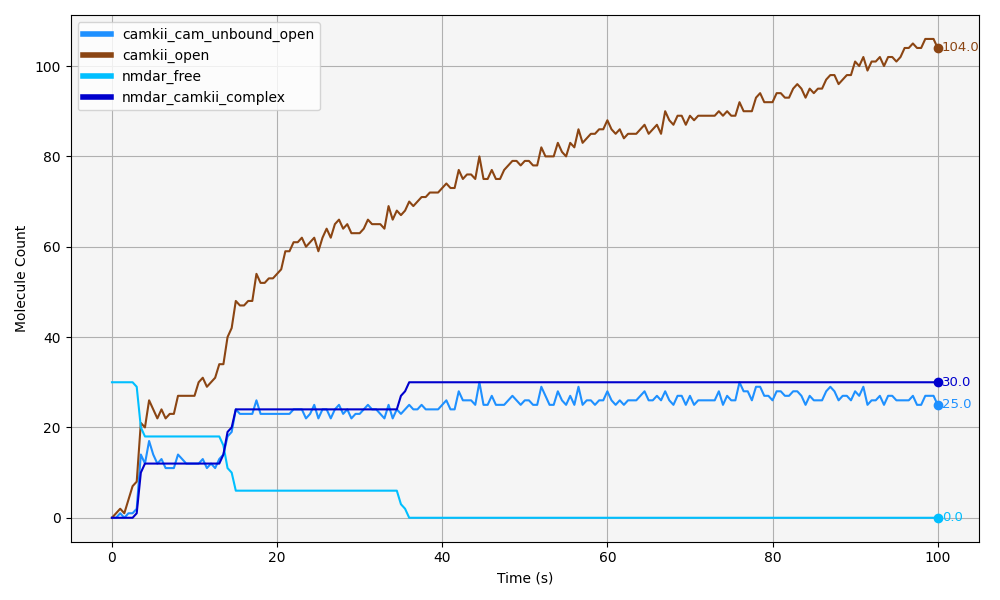
\includegraphics[keepaspectratio]{40-results-figures/WT/camkii-open-nmdar.png}}

}

\subcaption{\label{fig-camkii-opening-nmdar}}

\end{minipage}%

\caption{\label{fig-camkii-open}Stabilisation of CaMKII in the Open
Conformation.}

\end{figure}%

\subsection{CaMKII subunits remain open and autophosphorylate at T286
upon NMDAR binding, regardless of CaM
binding}\label{camkii-subunits-remain-open-and-autophosphorylate-at-t286-upon-nmdar-binding-regardless-of-cam-binding}

Next we look at total number of CaMKII subunits phosphorylated at T286.
Camkii\_t286p reflects the full amount of T286-phosphorylated CaMKII,
irrespective of any other concurrent molecular states. All CaMKII
subunits categorised as camkii\_t286p are necessarily in the open
conformation. Therefore, camkii\_t286p represents a subset of the
camkii\_open population (Figure~\ref{fig-subsets-of-open-t286p1_p0}).
This is consistent with both the model's coding and biological evidence,
as phosphorylation at T286 locks CaMKII in an autonomously active, open
conformation by preventing the regulatory segment from re-binding to the
catalytic domain, which physically prevents closing of the subunit.

Out of the 104 CaMKII subunits that are open at the end of the
simulation, 45 are found to be phosphorylated at T286
(Figure~\ref{fig-subsets-of-open-t286p1_p0}), and the rest (104 - 45 =
59) are therefore not phosphorylated at this site. This indicates that
approximately half of the open CaMKII subunits are in a
T286-phosphorylated state.

Of the 45 T286-phosphorylated CaMKII subunits, a subset of 25 are found
to be bound to NMDARs (pink line: camkii\_t286p1\_bound\_nmdar as shown
in Figure~\ref{fig-camkii-t286p-nmdar-b}). The difference between these
two molecules, corresponds to the number of CaMKII molecules that are
T286-phosphorylated but not associated with NMDARs. This is, out of all
the CaMKII subunits that are phosphorylated at T286, about half can be
found bound to NMDARs, and the other half is not.
Figure~\ref{fig-subsets_nmdar-t268p} further demonstrates that the
majority of CaMKII subunits bound to NMDARs and phosphorylated at T286
are free from CaM. This complements observations in
Figure~\ref{fig-camkii-t286p-nmdar-b}, where 25 CaMKII subunits are both
T286-phosphorylated and bound to NMDARs, of which 23 are CaM-free and
only 2 remain CaM-bound by the end of the simulation.

Further, within the population of T286-phosphorylated CaMKII that is
also bound to NMDARs (pink line: camkii\_t286p1\_bound\_nmdar), only a
very small number of subunits remain bound to CaM
(Figure~\ref{fig-subsets_nmdar-t268p}). Thus, the majority of CaMKII
subunits that are bound in a NMDAR/CaMKII complex are both
phosphorylated at T286 and free from CaM (which is consistent with
literature, as further discussed in Chapter~\ref{sec-discussion}). This
is, once CaMKII is bound to the NMDARs, the holoenzyme subunits can
remain open, and autophosphorylate even in the absence of CaM.

\begin{figure}[H]

\centering{

\pandocbounded{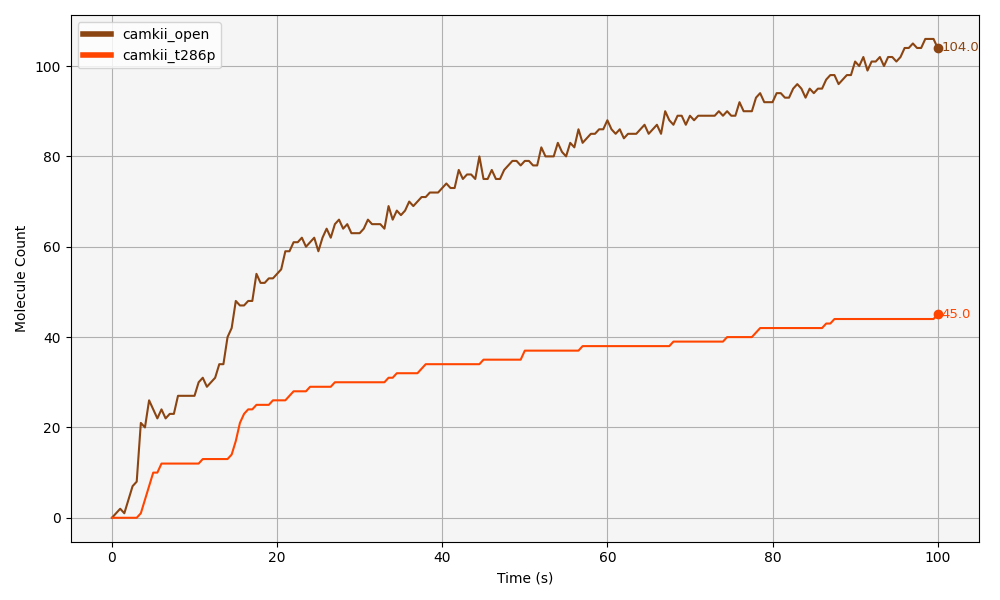
\includegraphics[keepaspectratio]{40-results-figures/WT/subsets-of-open-t286p1_p0.png}}

}

\caption[CaMKII open and T286
phosphorylated]{\label{fig-subsets-of-open-t286p1_p0}Approximately half
of CaMKII that is open (camkii\_open) is also phosphorylated at T286
(camkii\_t286p). The difference between 104 and 45 is the amount of
CaMKII that is open and unphosphorylated at T286.}

\end{figure}%

\begin{figure}[H]

\centering{

\pandocbounded{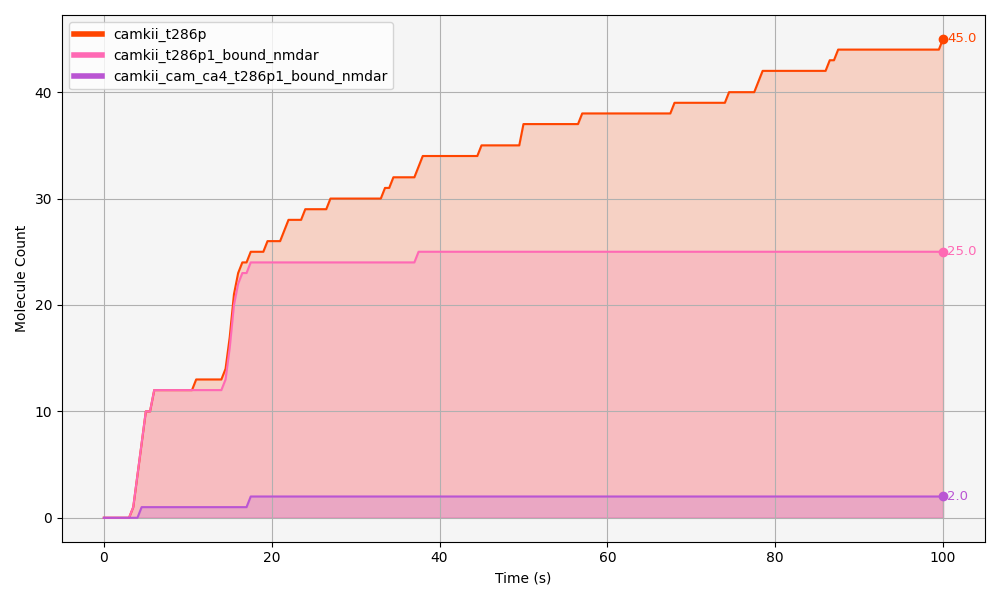
\includegraphics[keepaspectratio]{40-results-figures/WT/camkii-t286p.png}}

}

\caption[CaMKII T286 phosphorylated and bound to
CaM]{\label{fig-camkii-t286p-nmdar-b}Approximately half of all
T286-phosphorylated CaMKII subunits (camkii\_t286p) are also bound to
NMDARs (camkii\_t286p\_bound\_nmdar) by the end of the simulation.}

\end{figure}%

\begin{figure}[H]

\centering{

\pandocbounded{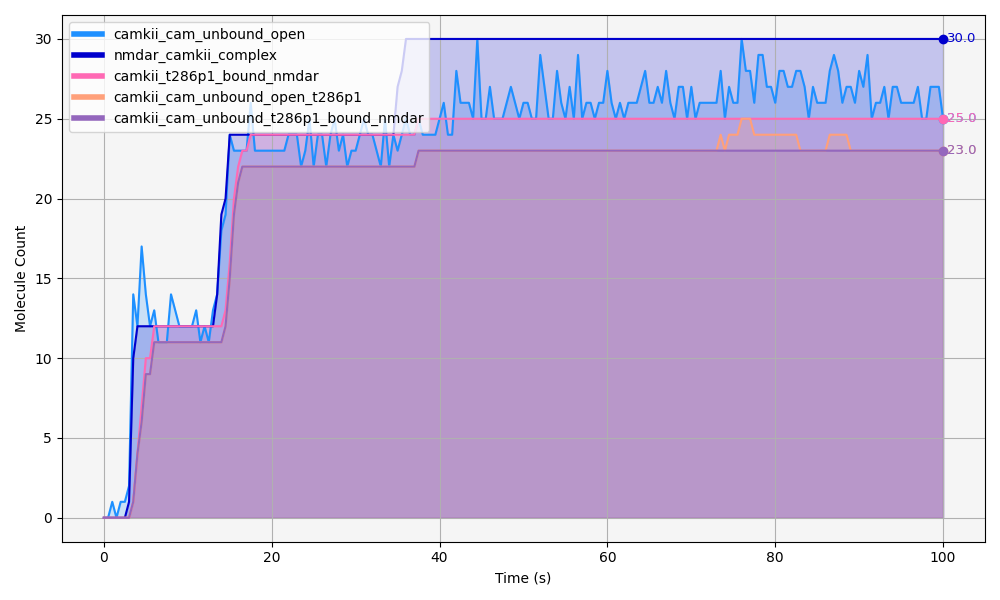
\includegraphics[keepaspectratio]{40-results-figures/WT/subsets_nmdar-t268p.png}}

}

\caption[Most CaMKII phosphorylated at T286 and bound to NMDARs is free
from CaM]{\label{fig-subsets_nmdar-t268p}Most CaMKII phosphorylated at
T286 and bound to NMDARs (camkii\_t286p1\_bound\_nmdar) is free from CaM
(camkii\_cam\_unbound\_t286p1\_nmdar).}

\end{figure}%

\subsection{NMDAR binding is the primary driver of T286
phosphorylation}\label{nmdar-binding-is-the-primary-driver-of-t286-phosphorylation}

As explained in Section~\ref{sec-cam-binding-and-t286-p}, we use a
`conformational selection' approach to modelling CaMKII activation,
where CaMKII can exist in both open and closed states independently, and
CaM selectively binds to and stabilizes the open conformation, without
\emph{inducing} a conformational change. In order to understand how CaM
is interacting with CaMKII T286 phosphorylation, we look at
Figure~\ref{fig-subsets-of-camkii-t286p-cam-binding}. Here we can see
that among all CaMKII subunits phosphorylated at T286, approximately
half (23 molecules) are also bound to CaM, represented by the
peach-coloured trace \emph{``camkii\_cam\_ca4\_t286p1''}, while the
remaining half (22 molecules) are unbound from CaM (brown-coloured
trace: \emph{``camkii\_cam\_unbound\_open\_t286p1''}).

This indicates that, although CaM binding co-occurs with T286
phosphorylation, T286 is not necessarily more likely when subunits are
bound to CaM. In fact, subunits that are both CaM-bound and
T286-phosphorylated emerge more slowly during the simulation
(Figure~\ref{fig-subsets-of-camkii-t286p-cam-binding}), suggesting that
CaM binding is not the main event leading to the increase of initial
CaMKII T286 phosphorylation, but as we will see next, NMDAR binding is
(by keeping CaMKII subunits in their open conformation and allowing
subsequent T286 autophosphorylation).

T286-phosphorylated CaMKII which is free from CaM (peach-coloured line
in Figure~\ref{fig-xsubsets_nmdar-t268p}) corresponds in timing with the
formation of the CaMKII/NMDAR complex
(Figure~\ref{fig-subsets_nmdar-t268p}). This suggests that, once CaMKII
binds to NMDARs and its subunits are held in the open conformation,
autophosphorylation at T286 is further facilitated in the CaMKII
subunits that are part of the CaMKII/NMDAR complex.

Interestingly, a slight increase in the population of CaMKII free from
CaM and T286 phosphorylated is observed around 80 seconds. This rise
suggests that subunits of holoenzymes locked into the CaMKII/NMDAR
complex undergo further autophosphorylation of neighbouring subunits,
resulting in a momentary increase in CaMKII subunits that are free from
CaM and phosphorylated at T286.

\begin{figure}

\centering{

\pandocbounded{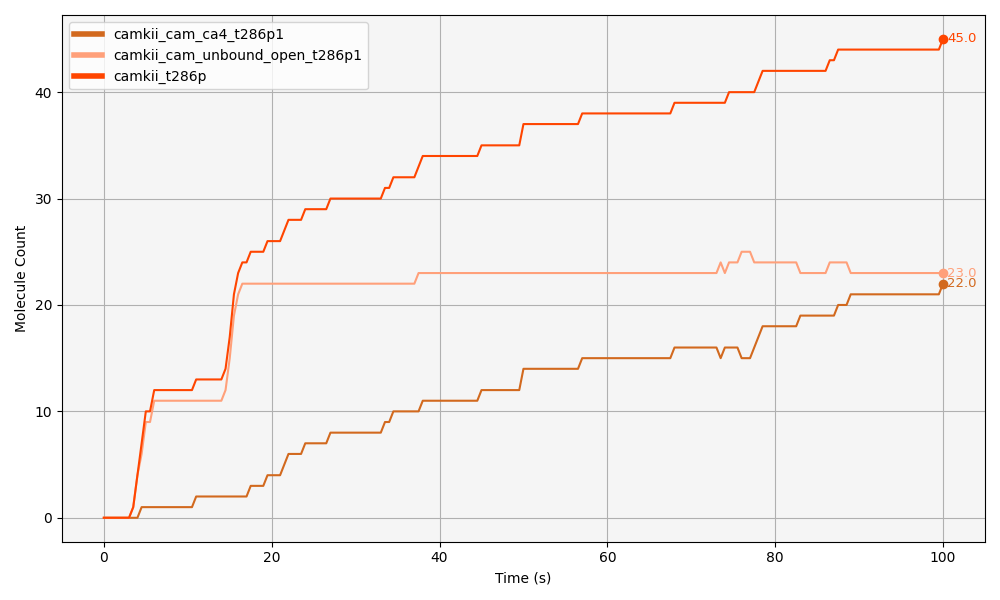
\includegraphics[keepaspectratio]{40-results-figures/WT/subsets-of-camkii-t286p-cam-binding.png}}

}

\caption{\label{fig-subsets-of-camkii-t286p-cam-binding}CaM binding is
not the main event leading to the increase of initial CaMKII T286
phosphorylation, as out of all the CaMKII that is T286 phosphorylated
(camki\_t286p), most of it first increases in a state that is free from
CaM (camkii\_cam\_unbound\_open\_t286p1), whereas CaMKII that is bound
to CaM and T286 phosphorylated (camkii\_cam\_ca4\_t286p1) increases more
slowly and later.}

\end{figure}%

\begin{figure}

\centering{

\pandocbounded{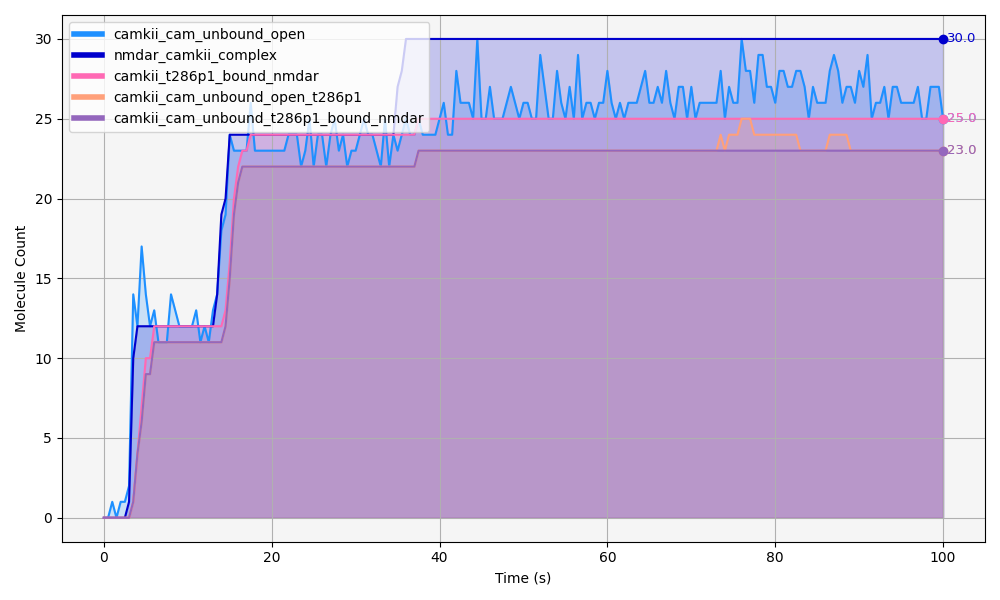
\includegraphics[keepaspectratio]{40-results-figures/WT/xsubsets_nmdar-t268p.png}}

}

\caption[Binding of CaMKII to NMDARs promotes and stabilizes the open
conformation of its subunits]{\label{fig-xsubsets_nmdar-t268p}Binding of
CaMKII to NMDARs promotes and stabilizes the open conformation of its
subunits, facilitating T286 autophosphorylation within the CaMKII/NMDAR
complex.}

\end{figure}%

\subsection{NMDAR binding also promotes CaMKII autophosphorylation at
T306
site}\label{nmdar-binding-also-promotes-camkii-autophosphorylation-at-t306-site}

Phosphorylation at the T306 site is known to occur at a slower rate than
phosphorylation at T286 {[}\citeproc{ref-chang2017CaMKII}{153},
\citeproc{ref-otmakhov2015Fast}{475}{]}, and this is reflected in the
model outputs. A total of 25 CaMKII subunits become phosphorylated at
T306 over the course of the simulation (burgundy trace: camkii\_t306p in
Figure~\ref{fig-t306p}), of which 21 are bound to the NMDAR (golden
trace:camkii\_cam\_unbound\_t306p1\_bound\_nmdar in
Figure~\ref{fig-t306p}) ---indicating that approximately 84\% of
T306-phosphorylated subunits are part of NMDAR complexes.

Moreover, the accumulation of doubly phosphorylated subunits (T286P and
T306P; here referred to as CaMKII\_PP, hot pink trace in
Figure~\ref{fig-t306p}) appears to track closely with the rate of T306
phosphorylation. This indicates that T306 phosphorylation typically
follows T286 phosphorylation, particularly during the earlier stages of
the simulation. This behaviour is consistent with both the modelled
mechanisms and findings reported in the literature
{[}\citeproc{ref-pi2010Autonomousa}{196}{]}.

\begin{figure}[H]

\centering{

\pandocbounded{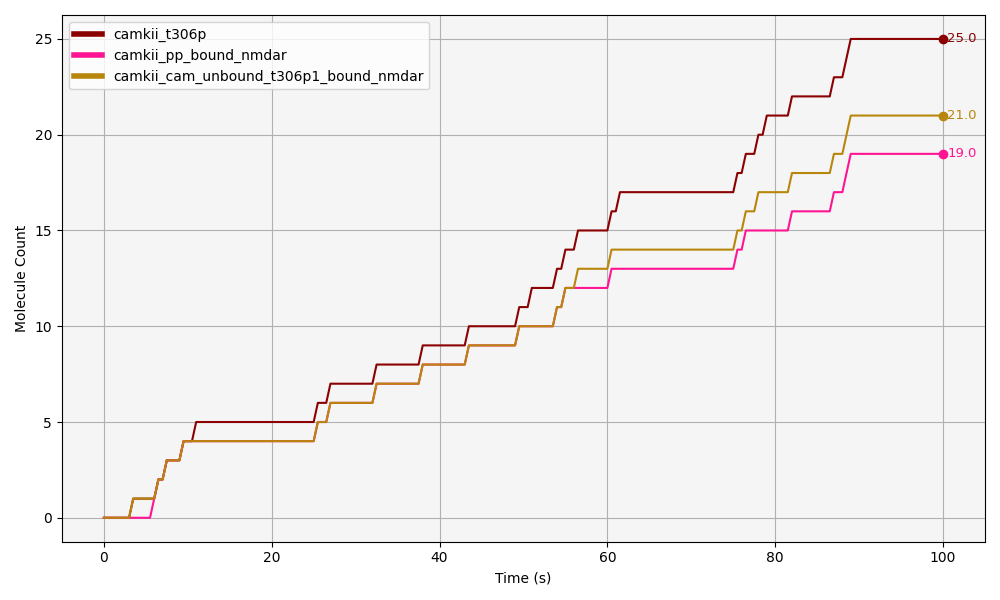
\includegraphics[keepaspectratio]{40-results-figures/WT/t306p.png}}

}

\caption[T306 phosphorylation can occur and persist independently of
T286]{\label{fig-t306p}At later stages, T306 phosphorylation can occur
and persist independently of T286 in CaMKII that is bound to
NMDARs.Initially, most of the CaMKII phosphorylated at T306
(camkii\_t306p) is also phosphorylated at T286---i.e., it is in the
doubly phosphorylated state (camkii\_pp\_bound\_nmdar). This indicates
that early T306 phosphorylation often coincides with T286
phosphorylation. After 60 seconds, the amount of CaMKII that is bound to
NMDARs and phosphorylated only at T306
(camkii\_cam\_unbound\_t306p1\_bound\_nmdar\emph{) surpasses the doubly
phosphorylated form. }Saying cam\_unbound (CaM free) in this molecule
name is redundant as camkii that is t306p is necessarily free from CaM.}

\end{figure}%

Interestingly, after around 60 seconds, subunits that are solely
phosphorylated at T306 continue to increase above CaMKII\_PP
(Figure~\ref{fig-t306p}). This suggests that, at later stages in the
simulation, T306 phosphorylation can occur and persist independently of
T286 phosphorylation. Extending the simulation time may offer further
insights into this dynamic, as it could support the biological
hypothesis that initial T286 phosphorylation enables subsequent T306
phosphorylation, but that T306P can then be maintained even in the
absence of T286 phosphorylation
{[}\citeproc{ref-bhattacharyya2020Flexible}{175},
\citeproc{ref-hanson1992Inhibitory}{195},
\citeproc{ref-pi2010Autonomousa}{196}{]}.

Furthermore, T306 phosphorylation follows NMDAR binding dynamics
closely. As shown in Figure~\ref{fig-t306p-nmdar-binding}, CaMKII
subunits initially bind to NMDARs in an unphosphorylated T306 state
(slate-green: camkii\_t306p0\_bound\_nmdar in
Figure~\ref{fig-t306p-nmdar-binding}). Once the CaMKII--NMDAR complex
reaches equilibrium, levels of T306 phosphorylation increase
correspondingly, as unphosphorylated T306 decreases.

\begin{figure}[H]

\centering{

\pandocbounded{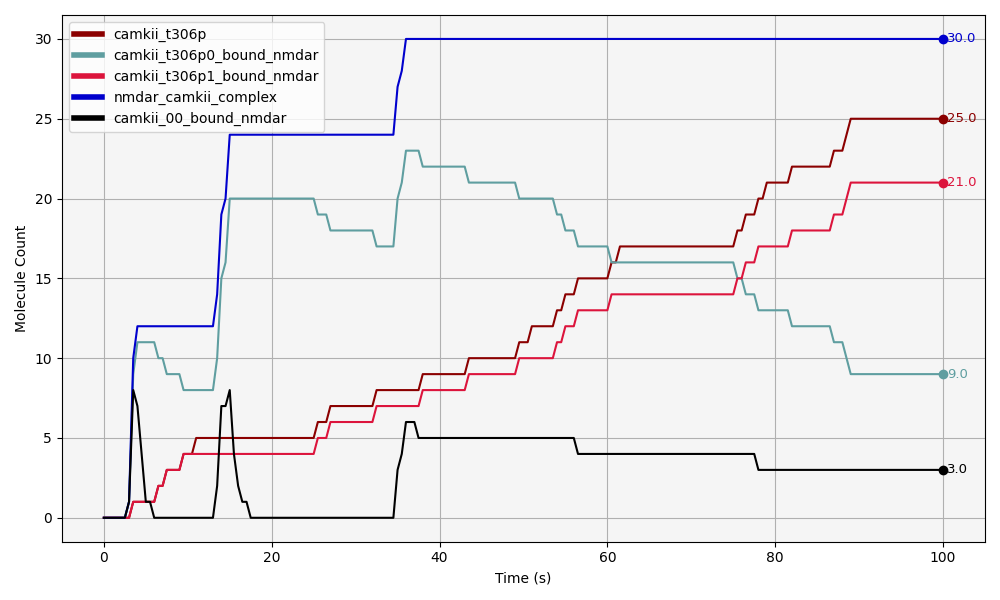
\includegraphics[keepaspectratio]{40-results-figures/WT/t306p-nmdar-binding.png}}

}

\caption[CaMKII binds unphosphorylated to
NMDARs]{\label{fig-t306p-nmdar-binding}CaMKII binds unphosphorylated to
NMDARs (camkii\_00\_bound\_nmdar). T286 phosphorylation ensues, followed
by an increase in T306 phosphorylation (camkii\_t306p1\_bound\_nmdar)
-and a T306 unphosphorylated state decrease
(camkii\_t306p0\_bound\_nmdar). All these molecules are a subset of
CaMKII bound to NMDARs (nmdar\_camkii\_complex).}

\end{figure}%

In the final phase of CaMKII binding to NMDARs, after approximately 40
seconds ---when all NMDARs are saturated, T306 phosphorylation continues
to rise. This is likely supported by the concurrent increase in T286
phosphorylation, and by a decrease in CaM binding to CaMKII subunits
already bound to NMDARs. This aligns with expectations, as CaM binding
and T306 phosphorylation are mutually exclusive processes ---CaM must be
unbound for T306 phosphorylation to occur. Therefore, as the model shows
a decrease in CaM binding to CaMKII subunits that are already part of
the CaMKII--NMDAR complex, the opportunity for T306 phosphorylation
increases. In other words, the less CaM is bound to CaMKII subunits, the
more likely it is that T306 can become phosphorylated, and the less
likely CaM is to bind.

Figure~\ref{fig-t306p-nmdar-binding} shows three distinct peaks, each
representing CaMKII subunits that are in the ``p00'' state --- meaning
they are not phosphorylated at either T286 or T306. This pattern
highlights three important insights. First, CaMKII binds to NMDARs
before any phosphorylation has occurred. Second, although
phosphorylation is not required for binding, once CaMKII is incorporated
into an NMDAR complex, autophosphorylation becomes more likely. Third,
phosphorylation at T306 follows phosphorylation at T286, following a
sequential phosphorylation mechanism as expected.

These findings show that the formation of CaMKII-NMDAR complexes does
not depend on prior phosphorylation at T286. However, once T286
phosphorylation occurs, it can initiate a cascade of further
autophosphorylation events, including at T306, within the same
NMDAR/CaMKII complex. Previous studies have shown that CaMKII does not
need to be phosphorylated at T286 in order to bind to NMDARs or to
perform its catalytic functions. That said, phosphorylation at T286 can
modulate or enhance both the binding affinity and the enzymatic activity
of CaMKII, making it an important regulatory step rather than an
absolute requirement.

\section{Analysis of the T286 and CaMKII/NMDAR binding mutant
models}\label{analysis-of-the-t286-and-camkiinmdar-binding-mutant-models}

The T286 MT model is similar biologically to the CaMKII T286A MT, in
which the critical autophosphorylation site T286 is substituted with
alanine, preventing phosphorylation at this site. This mutation has been
extensively characterised in both \emph{in vitro} biochemical assays and
\emph{in vivo} using mice that were genetically modified. T286A mutation
has been shown to impair LTP and spatial learning in rodents
{[}\citeproc{ref-colbran2004Protein}{147},
\citeproc{ref-miller1986Regulation}{187},
\citeproc{ref-coultrap2010CaMKIIa}{188},
\citeproc{ref-lou1986Activation}{467}{]}. This computational
implementation allows investigation into how the loss of T286
phosphorylation alters CaMKII dynamics and downstream NMDAR interactions
under different stimulation conditions. In the T286 MT model, this
mutation is represented by setting reaction rule \#8 to zero
(Figure~\ref{fig-tbl-1}), so phosphorylation can not happen.

The NMDAR/CaMKII binding MT model simulates a mutation that disrupts the
interaction between CaMKII and the GluN2B subunit of NMDARs. This
disruption can be achieved through mutations in either CaMKII or GluN2B,
preventing their binding without necessarily altering other functions
such as kinase activity {[}\citeproc{ref-sanhueza2013CaMKII}{9}{]}. A
well-characterized example is the CaMKII I205K mutation, where
isoleucine is replaced by lysine. This substitution significantly
impairs binding to GluN2B while leaving kinase activity intact
{[}\citeproc{ref-bayer2001Interactiona}{127}{]}. Experimental evidence
shows that this mutation also reduces CaMKII accumulation at synapses
following LTP induction {[}\citeproc{ref-bayer2001Interactiona}{127}{]}.
In the CaMKII/NMDAR MT model, this binding disruption is represented by
setting reaction rule \#12 to zero (Figure~\ref{fig-tbl-1}), so NMDAR
and CaMKII binding can not proceed.

The following analysis compares WT simulations with those of the two MT
models. The total number of simulation runs for each group is as
follows: WT (N = 9), T286 MT (N = 9), and CaMKII/NMDAR MT (N = 4).
T-tests and one-way ANOVAs were performed after testing for normality of
the datasets using the Shapiro-Wilk test.

Simulations were conducted under identical parameters across all
conditions (see Figure~\ref{fig-molecule-concentrations} for initial
molecule release and Figure~\ref{fig-tbl-1} for reaction rates), except
for two CaMKII/NMDAR MT runs, as I explain below, which were part of
preliminary tests involving a different CaMKII release state. Aside from
this, the only intended differences between groups were the
modifications to the relevant reaction rules described above.

The reduced number of simulations for the CaMKII/NMDAR MT model resulted
from a human error during file execution, which will be explored in
greater detail in the discussion section below. Due to this error, only
four usable simulation runs were available for this model. It is
important to note that, while all other simulation groups released
CaMKII in its open state, the CaMKII/NMDAR MT group includes two runs
with CaMKII released in the closed state and two with CaMKII released in
the open state. These files, originally generated during preliminary
testing (data not shown), were the only available usable runs for this
condition due to the aforementioned error. As no substantial differences
in simulation outcomes were observed between the two release states, all
four runs were retained in the analysis. This detail is provided here
for transparency.

\subsection{NMDAR binding stabilizes CaMKII open conformation more
readily than T286
phosphorylation}\label{nmdar-binding-stabilizes-camkii-open-conformation-more-readily-than-t286-phosphorylation}

Having established the simulation conditions for each model, we now
present quantitative comparisons between WT and MT simulations across
key molecular outputs. A primary focus of this analysis is the extent of
CaMKII opening, as this conformational state is influenced by both T286
phosphorylation and binding to NMDARs. Given that both of these
interactions promote and stabilise the open conformation of CaMKII, it
was expected that disrupting either mechanism, through mutation at T286
or impairment of NMDAR binding, would lead to a reduction in CaMKII
opening.

Figure~\ref{fig-camkii_open_anova} displays the results of an ANOVA,
with an F-statistic of 36.327, indicating a substantial difference
between the group means relative to the variation within each group.
Further, the associated p-value of \(3.219 \times 10^{-7}\) indicates a
very low probability that the observed differences between the groups
are due to random chance.

Both mutations significantly decreased CaMKII opening relative to the WT
control. The reduction observed in the T286\_MT group was modest, with a
mean of 100 compared to 109 in the WT group, but statistically
significant (p \textless{} 0.05), supporting the role of T286
phosphorylation in stabilising the open conformation of CaMKII. These
results were expected, as abolishing T286 phosphorylation means
decreasing the chances of CaMKII subunits being kept in their open
conformation via this mechanism.

The NMDAR\_CaMKII\_MT group exhibited a much more pronounced and highly
significant reduction in CaMKII opening compared to the WT group (p
\textless{} 0.0001). As expected, reduced binding to NMDARs corresponds
to a decreased likelihood of CaMKII remaining in its open conformation.
Interestingly, CaMKII opening in the NMDAR\_CaMKII\_MT group was not
only significantly lower than in the WT group, but also lower than in
the T286\_MT group (p \textless{} 0.0001). These findings reinforce the
idea that NMDAR binding plays a central role in maintaining CaMKII in
its open state in our simulations. While T286 phosphorylation is also
important, it is the disruption of CaMKII/NMDAR binding that most
strongly impacts CaMKII opening levels.

\begin{figure}[H]

\centering{

\pandocbounded{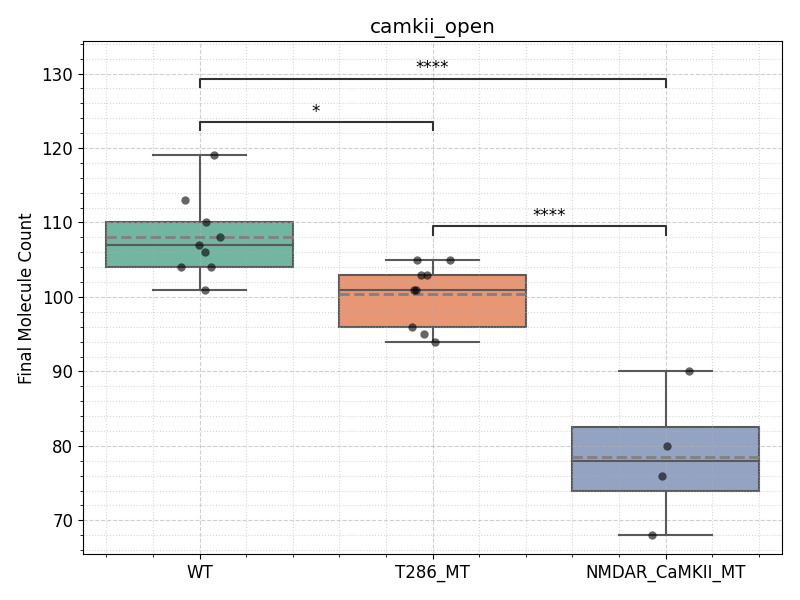
\includegraphics[keepaspectratio]{40-results-figures/statistics/camkii_open_anova.png}}

}

\caption[Both the T286 MT and the NMDAR/CaMKII binding MT exhibit
significantly lower levels of CaMKII opening compared to
WT]{\label{fig-camkii_open_anova}Both the T286 MT (T286\_MT) and the
NMDAR/CaMKII binding MT (NMDAR\_CaMKII\_MT) exhibit significantly lower
levels of CaMKII opening compared to WT, with the largest reduction
observed in the NMDAR\_CaMKII\_MT condition. Final molecule counts for
camkii\_open are shown for each simulation run (dots), with group-level
distributions represented as boxplots. Solid lines represent medians,
and dashed lines represent means. Statistical comparisons were performed
using one-way ANOVA followed by Tukey's HSD post hoc test. Asterisks
indicate levels of statistical significance from Tukey's HSD post hoc
test: p \textless{} 0.05 (*), p \textless{} 0.001 (**), and p
\textless{} 0.0001 (****). ANOVA F-statistic between groups = 36.327,
and \(p = 3.219 \times 10^{-7}\).}

\end{figure}%

\subsection{Autophosphorylation at T286 promotes CaM binding but NMDAR
binding does
not}\label{autophosphorylation-at-t286-promotes-cam-binding-but-nmdar-binding-does-not}

Next, I aimed to examine whether CaM binding to CaMKII was affected
across the three models. Given the expected reduction in CaMKII opening,
I expected that this decrease might also result in reduced CaM binding
in both MT models. Specifically, I wanted to explore how CaM binding is
related to both T286 phosphorylation and NMDAR/CaMKII binding.

As shown in Figure~\ref{fig-CaMKII_CaM_Ca4_anova}, total CaMKII bound to
CaM (camkii\_cam\_ca4) was significantly reduced only in the T286 MT.
The F-value of 4.668 indicates that the variance \emph{between} groups
(i.e., how much the CaM binding values differ between the WT, T286\_MT,
and NMDAR/CaMKII\_MT) is considerably larger than the variance
\emph{within} groups (i.e., how much individual data points vary within
each group). In other words, the groups are not just randomly different;
the differences between the groups are meaningful and consistent. The
significant reduction in CaM binding in the T286 MT (p \textless{}
0.05), and the lack of difference in the NMDAR/CaMKII MT compared to WT,
suggests that T286 phosphorylation influences CaM binding to CaMKII by
keeping it in the open state. On the other hand, NMDAR binding does not
appear to have a similar effect.

These findings were initially unexpected, as I had anticipated that
reduced CaMKII opening in both MTs might affect CaM binding in both
models. However, the results are actually consistent with the underlying
mechanisms that we had previously observed. In the WT model, CaM binding
and NMDAR binding to CaMKII subunits appeared to be independent
processes. Notably, the majority of CaMKII bound to NMDARs did not
interact with CaM. This independence between NMDAR binding and CaM
binding to CaMKII helps explain why the NMDAR/CaMKII MT, which disrupts
NMDAR binding, does not significantly affect CaM binding. Since NMDAR
binding and CaM binding to CaMKII are independent events, disrupting
NMDAR binding does not impact the ability of CaMKII to bind to or
release CaM. In contrast, the T286 mutation does lead to a reduction in
CaM binding, highlighting the specific role of T286 phosphorylation in
regulating CaM binding.

\begin{figure}[H]

\centering{

\pandocbounded{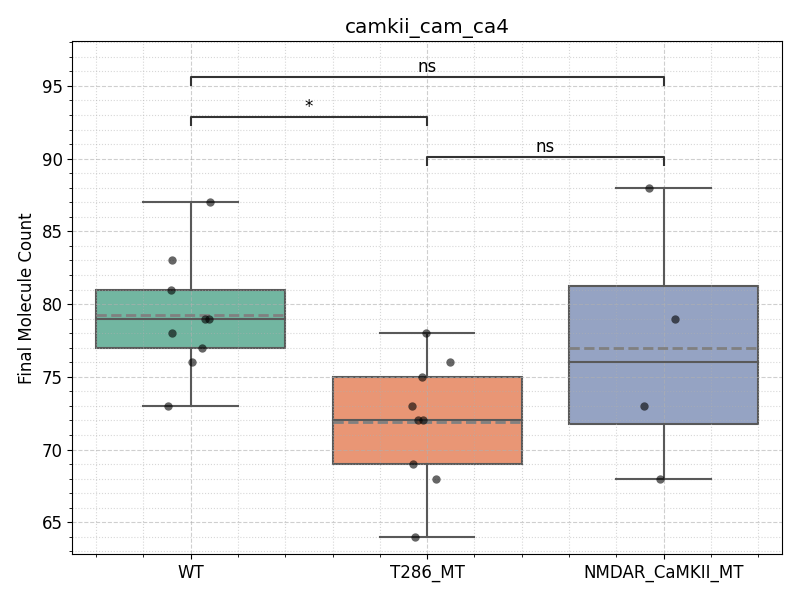
\includegraphics[keepaspectratio]{40-results-figures/statistics/CaMKII_CaM_Ca4_anova.png}}

}

\caption[CaM binding to CaMKII is significantly reduced only with the
loss of T286 phosphorylation]{\label{fig-CaMKII_CaM_Ca4_anova}CaM
binding to CaMKII is significantly reduced only with the loss of T286
phosphorylation. Final molecule counts for camkii\_cam\_ca4 are shown
for each simulation run (dots), with group-level distributions
represented as boxplots. Solid lines represent medians, and dashed lines
represent means. The T286 MT (T286\_MT) shows a significant reduction in
CaM-bound CaMKII compared to WT (p \textless{} 0.05), whereas no
significant difference (`ns') is observed between WT and the
NMDAR/CaMKII MT (NMDAR\_CaMKII\_MT), or between the two MT groups.
Statistical analysis was performed using one-way ANOVA (F = 4.668, p =
0.022), followed by Tukey's HSD post hoc test.}

\end{figure}%

\subsection{NMDAR binding is the main stabiliser of CaMKII's open
state}\label{nmdar-binding-is-the-main-stabiliser-of-camkiis-open-state}

To further explore how NMDARs and T286 phosphorylation affect CaMKII
opening, I looked at the amount of CaMKII subunits that remain free from
CaM and are kept in their open state (denoted as
CaMKII--CaM\_unbound\_open, Figure~\ref{fig-camkii_cam_unbound_open}). I
observed a significant decrease in this molecule count in the
NMDAR/CaMKII binding MT. As discussed previously, in the WT model,
NMDARs play an active role in stabilizing CaMKII in its open state, even
in the absence of CaM. This means that, in this model, NMDARs are
crucial for maintaining CaMKII in its open form, free from calmodulin.
When this stabilizing mechanism is disrupted in the NMDAR/CaMKII mutant,
less CaMKII remains in the open state without CaM, because the NMDAR
binding, which normally helps keep the CaMKII subunits open and
CaM-free, is no longer functioning. As a result, there is a reduction in
the amount of CaMKII remaining in its open state. Conversely, in the
T286 mutant model, the ability of NMDARs to keep CaMKII in its open,
CaM-free state is still intact, which explains why this aspect remains
unaffected in this model.

\begin{figure}[H]

\centering{

\pandocbounded{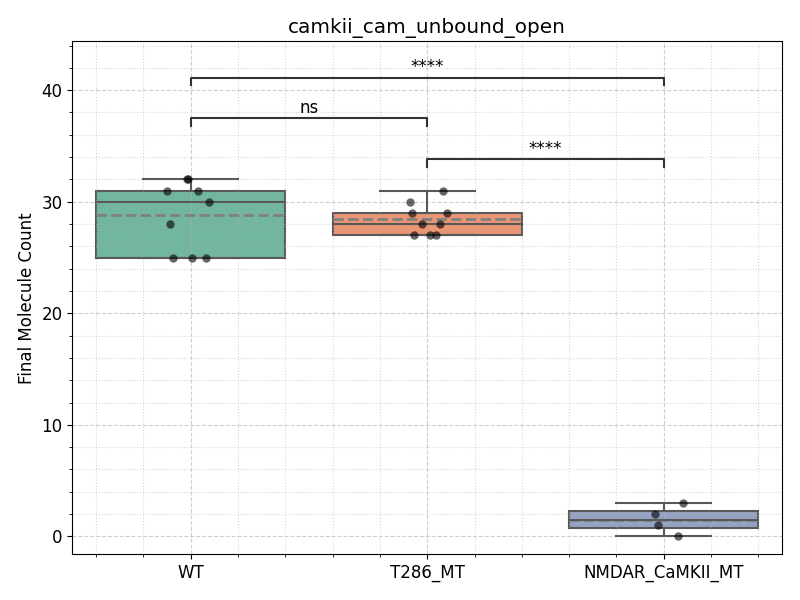
\includegraphics[keepaspectratio]{40-results-figures/statistics/camkii_cam_unbound_open.png}}

}

\caption[NMDAR binding is crucial for maintaining CaMKII in its open,
CaM-free state]{\label{fig-camkii_cam_unbound_open}NMDAR binding is
crucial for maintaining CaMKII in its open, CaM-free state
(camkii\_cam\_unbound\_open). Boxplot shows final molecule counts for
camkii\_cam\_unbound\_open across WT, T286 phosphorylation mutant
(T286\_MT), and NMDAR/CaMKII binding mutant (NMDAR\_CaMKII\_MT) models.
Individual simulation runs are represented as dots. Boxes represent the
interquartile range, solid lines show medians, and dashed lines show
group means. A one-way ANOVA revealed a significant group effect (F =
236.180, \(p = 3.80 \times 10^{-14}\)), with post hoc Tukey's HSD tests
indicating significantly fewer CaMKII molecules in this state in the
NMDAR/CaMKII mutant compared to both WT and T286\_MT (**p \textless{}
0.001). No significant difference was observed between WT and T286\_MT.}

\end{figure}%

\subsection{NMDAR binding stabilizes CaMKII open conformation and drives
T286 and T306
phosphorylation}\label{nmdar-binding-stabilizes-camkii-open-conformation-and-drives-t286-and-t306-phosphorylation}

Since NMDARs play an essential role in keeping CaMKII subunits open and
free from CaM (as shown by the CaMKII\_cam\_unbound\_open data), this
opens up the question of whether T286 phosphorylation, which is a key
event for CaMKII activation, is also influenced by NMDAR signalling. In
the WT model, we observed that CaMKII subunits bind to NMDARs in an
unphosphorylated state, and T286 phosphorylation is subsequently
stabilized once these subunits associate with NMDARs, even in the
absence of CaM. What is more, NMDAR binding was identified as the key
event leading to T286 phosphorylation, as it helps maintain CaMKII in
its open conformation, thus enabling T286 autophosphorylation.
Consequently, in the NMDAR/CaMKII binding mutant, where NMDAR-CaMKII
interaction is disrupted, we expect T286 phosphorylation to be
significantly reduced due to the loss of this stabilisation mechanism.
As expected, in the NMDAR/CaMKII binding MT, we observed a significant
reduction in T286 phosphorylation, confirming the importance of
NMDAR-CaMKII binding in T286 autophosphorylation
(Figure~\ref{fig-camkii_t286p_nmdarMT}).

Further, as previously observed in the WT model, phosphorylation at T306
was promoted following T286 phosphorylation in CaMKII subunits already
bound to NMDARs, suggesting that NMDAR association is a key upstream
event driving T306 phosphorylation. Looking at
Figure~\ref{fig-t306p_anova}, we can see that T306 phosphorylation is
significantly reduced in the NMDAR/CaMKII mutant model compared to both
the WT and the T286 mutant, indicating that indeed NMDAR binding is
important for T306 phosphorylation. Interestingly, the T286 mutant does
not show a significant reduction in T306 phosphorylation relative to WT.
Given that in the WT model T306 phosphorylation typically follows T286
phosphorylation, one might expect the T286 mutant to also exhibit
reduced T306 levels. However, these results suggest that T306
phosphorylation can still occur independently of prior T286
phosphorylation, highlighting the dominant role of NMDAR binding in
promoting the T306 phosphorylation event. The biological significance of
these results is further explored in the discussion section below.

\begin{figure}[H]

\centering{

\pandocbounded{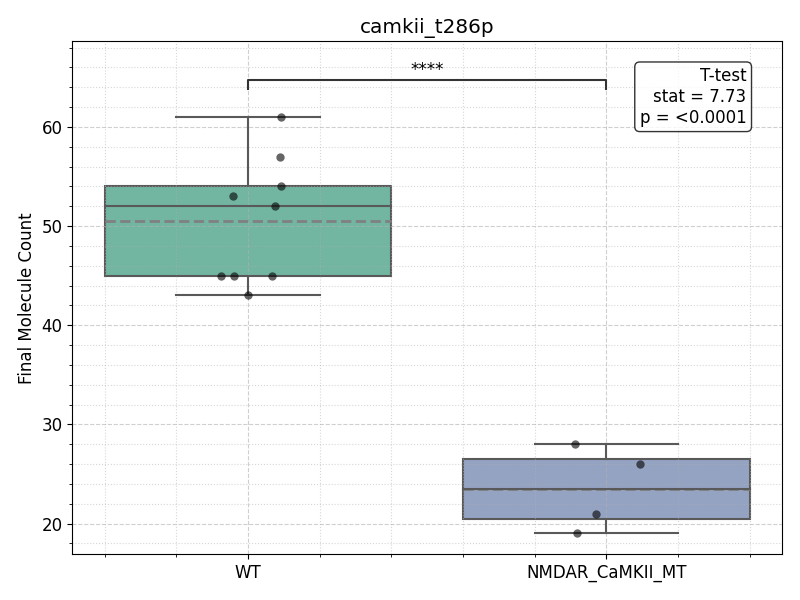
\includegraphics[keepaspectratio]{40-results-figures/statistics/camkii_t286p_nmdarMT.png}}

}

\caption[NMDAR binding is critical for promoting T286 phosphorylation of
CaMKII]{\label{fig-camkii_t286p_nmdarMT}NMDAR binding is critical for
promoting T286 phosphorylation of CaMKII. Individual simulation runs are
shown as dots; boxes indicate the interquartile range, with solid lines
denoting the median and dashed lines the mean. A two-tailed t-test
revealed a highly significant reduction in T286-phosphorylated CaMKII in
the NMDAR mutant (t = 7.73, p \textless{} 0.0001, ***), consistent with
the proposed mechanism where NMDAR binding stabilizes CaMKII in an open
conformation that favours autophosphorylation at T286.}

\end{figure}%

\begin{figure}[H]

\centering{

\pandocbounded{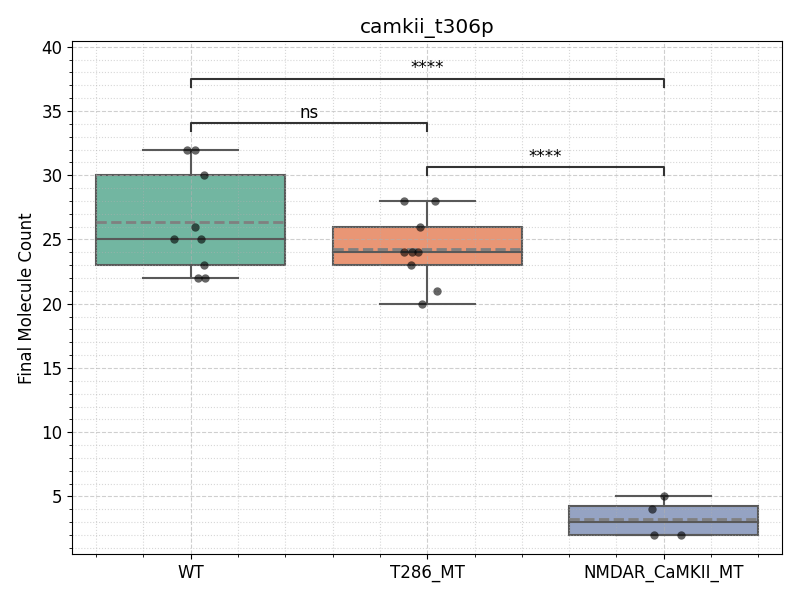
\includegraphics[keepaspectratio]{40-results-figures/statistics/t306p_anova.png}}

}

\caption[NMDAR binding is critical for T306 phosphorylation of
CaMKII]{\label{fig-t306p_anova}NMDAR binding is critical for T306
phosphorylation of CaMKII, while T286 phosphorylation has no significant
effect. Boxplot showing final camkii\_t306p molecule counts for WT, T286
mutant (T286\_MT), and NMDAR/CaMKII binding mutant (NMDAR\_CaMKII\_MT)
models. Individual simulation runs are shown as dots; boxes indicate the
interquartile range, with solid lines denoting the median and dashed
lines the mean. A one-way ANOVA revealed a significant overall effect (F
= 77.035, p = 7.674e--10), with Tukey's HSD post hoc test confirming
significantly reduced T306 phosphorylation in the NMDAR\_CaMKII\_MT
compared to both WT and T286\_MT (***), while the difference between WT
and T286\_MT was not statistically significant (ns). This suggests that
NMDAR-CaMKII interactions, but not T286 phosphorylation status, are
critical for enabling T306 phosphorylation.}

\end{figure}%

\subsection{T286 phosphorylation does not influence the binding of
CaMKII to
NMDARs}\label{t286-phosphorylation-does-not-influence-the-binding-of-camkii-to-nmdars}

As shown in Figure~\ref{fig-nmdar_MTvsWT}, both the T286 mutant model
and the wild-type (WT) eventually plateau at 30 bound CaMKII/NMDAR
complexes. This indicates that, despite the absence of T286
phosphorylation in the mutant model, the number of CaMKII subunits bound
to NMDARs reaches the same final value as in the WT. This observation
further strengthens the idea that NMDAR binding plays a critical role in
promoting T286 phosphorylation of CaMKII, while the phosphorylation
state of T286 does not influence the ability of CaMKII to bind to
NMDARs. Furthermore, as observed in the WT runs above (refer back to
Figure~\ref{fig-t306p-nmdar-binding}), CaMKII can bind to NMDARs in an
unphosphorylated state, providing additional support for the conclusion
that, in the model used here, NMDAR binding is a key driver of T286
phosphorylation but not the other way around.

\begin{figure}[H]

\centering{

\pandocbounded{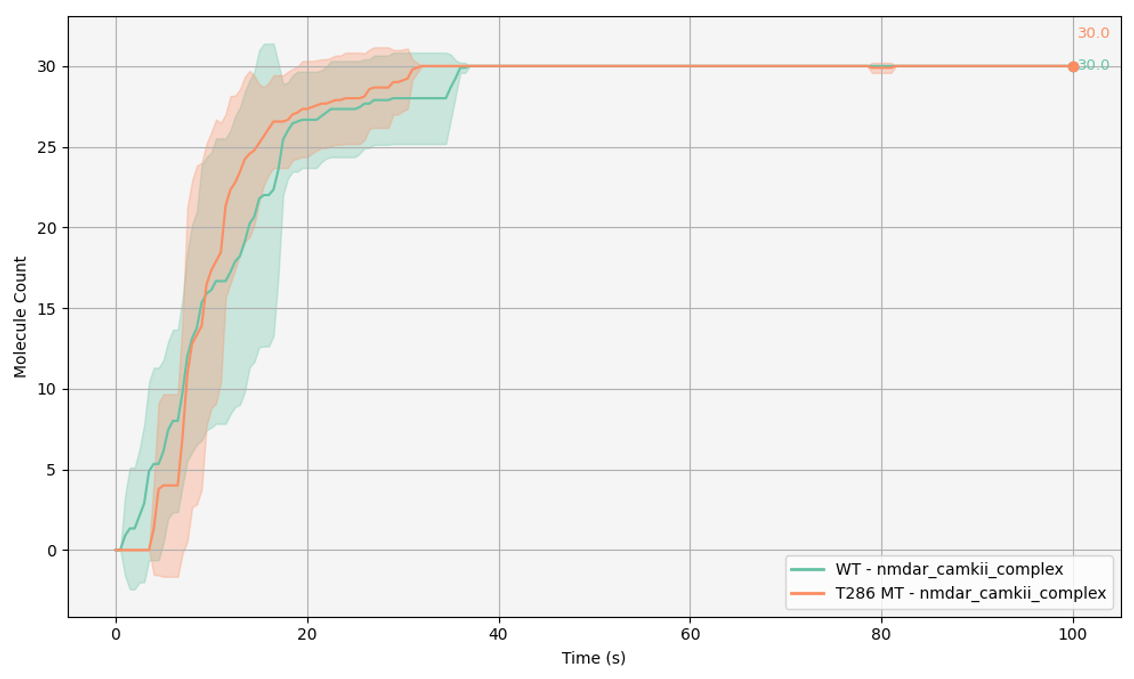
\includegraphics[keepaspectratio]{40-results-figures/statistics/nmdar_MTvsWT.png}}

}

\caption[NMDAR binding reaches full saturation in both WT and
NMDAR/CaMKII mutant models]{\label{fig-nmdar_MTvsWT}NMDAR binding
reaches full saturation in both WT and NMDAR/CaMKII mutant models.
Shaded areas indicate the standard deviation. Both models ultimately
reach a plateau of 30 bound CaMKII/NMDAR complexes. Due to the lack of
variability in the final molecule count (both reach 30 with no
variance), statistical comparisons of the end-point data are not shown.}

\end{figure}%

\bookmarksetup{startatroot}

\chapter{Summary of main findings: what have I done to tackle the aims
of this
PhD?}\label{summary-of-main-findings-what-have-i-done-to-tackle-the-aims-of-this-phd}

This PhD was structured around six main aims that guided both the
scientific and methodological progression of the project. Each aim built
on the previous one, moving from the development of a detailed
computational model of CaMKII--NMDAR interactions to the evaluation of
how these models can be made more transparent, reproducible, and
ethically grounded. The following section summarises the approaches
taken to achieve each aim and the key findings that emerged from them.

The first aim of this PhD was to develop a computational model of
CaMKII/NMDAR interactions. To achieve this, I built a model of CaMKII
activation and its interaction with NMDARs based on previously
established models (Chapter~\ref{sec-model-description}). The modelling
combined rule-based, stochastic, and spatial approaches using MCell, the
BioNetGen Language, and Python. The model was validated against
biological predictions to ensure that the simulation outcomes were
consistent with known experimental findings
(Chapter~\ref{sec-model-description}).

When determining appropriate parameter values for the model, those
governing calcium binding to CaM and CaM binding to CaMKII were
relatively straightforward to define, as they are well constrained by
previous experimental data and comprehensive reviews that have
identified parameter ranges consistent with biological observations.
However, significantly less experiments have focused on calculating and
providing kinetic parameters between CaMKII and NMDARs. Hence, I carried
out parameter exploration focusing on two pairs of reaction parameters
that were more uncertain yet critical for this study: (1) the kon/koff
values describing the CaMKII flicker of opening and closing, and (2) the
kon/koff values governing the binding of CaMKII to NMDARs, as discussed
in Section~\ref{sec-validating-model}. Notably,
{[}\citeproc{ref-pharris2019Multistate}{185}{]} and
{[}\citeproc{ref-leonard2002Regulation}{125}{]} provide parameter
estimates for CaMKII subunit opening/closing dynamics and CaMKII--NMDAR
binding, respectively. These reported values were ultimately adopted for
the model used in this PhD, as discussed in
Section~\ref{sec-validating-model}.

The second aim was to ensure that the computational model(s) created in
this PhD adhere to FAIR principles. This involved making the data and
model outputs \emph{Findable} by providing rich metadata and DOIs for
easy discovery; \emph{Accessible} by making resources openly available
with clear licenses and documentation; \emph{Interoperable} by using
standard formats and coding languages to support cross-platform
compatibility; and \emph{Reusable} by providing thorough documentation,
provenance of information, and licensing to enable future use. How these
principles are applied is discussed in
Chapter~\ref{sec-open-repro-chapter}.

The third aim focused on exploring how the functional states of CaMKII
contribute to stabilizing the CaMKII/NMDAR complex. In this model, each
subunit of the CaMKII dodecamer has specific states of interest,
including: opening/closing, T286 phosphorylation, T306 phosphorylation,
CaM binding, and NMDAR binding. By examining CaMKII in different
combinations of functional states, it was possible to investigate how
these configurations influenced the stability and dynamics of the
overall CaMKII/NMDAR complex over time. These analyses revealed that
most CaMKII bound to NMDARs is not associated with calmodulin,
suggesting that CaM binding is not required for stabilizing the complex.
Additionally, T286 phosphorylation appears to occur after initial
CaMKII/NMDAR binding, indicating that phosphorylation is not necessary
for binding but may be promoted by NMDAR interaction and help maintain
CaMKII in its open conformation.

Aim four was, in relation to aim three, to assess the impact of
disrupted CaMKII/NMDAR binding on CaMKII function. To investigate this,
I created an \emph{in silico} mutation in which CaMKII and NMDAR cannot
bind. Similarly, aim five focused on asessing the impact of disrupted
CaMKII phosphorylation on the CaMKII/NMDAR complex. For this latter aim,
I created another \emph{in silico} mutant model in which CaMKII cannot
be phosphorylated at T286.

The NMDAR/CaMKII mutant model exhibited a substantial decrease in the
proportion of CaMKII in its open, active conformation compared with both
the WT and T286 mutant models. This finding suggests that NMDAR binding
is integral to maintaining CaMKII in its open, active state. While the
T286 mutation also resulted in a reduction in CaMKII openness
---consistent with the established role of autophosphorylation at T286
in promoting autonomous kinase activity--- the effect was notably less
severe than that observed in the NMDAR-binding mutant. These results
align with previous reports demonstrating that CaMKII binding to the
GluN2B subunit of the NMDAR induces a conformational change that
sustains kinase activity even in the absence of T286 phosphorylation
{[}\citeproc{ref-rumian2024LTP}{211},
\citeproc{ref-cook2022CaMKIIb}{213}{]}. Furthermore, analysis of the
T286 mutant model revealed that the loss of phosphorylation at this site
alters CaMKII opening and CaM binding but does not disrupt CaMKII/NMDAR
binding. Collectively, these findings suggest that although T286
phosphorylation modulates CaMKII conformational dynamics and CaM
interactions, it is not required to stabilize the CaMKII/NMDAR complex
itself.

Previous studies have shown that prolonged CaMKII activation leads to
sustained association with NMDARs, and the present simulations are
consistent with this mechanism. The models indicate that NMDAR binding
is a key determinant of prolonged CaMKII activation, enabling the kinase
to remain in an open, active state even after CaM dissociation. This
behavior reproduces an emergent form of CaM trapping, wherein CaMKII
retains high CaM affinity as a result of its stabilized open
conformation. Although the models do not explicitly increase CaM
affinity following T286 phosphorylation, the phosphorylation event
appears to enhance CaM binding indirectly by stabilizing the active
state of the enzyme. Complementary to these structural findings, the
simulations reveal that NMDAR binding not only maintains CaMKII in an
open state but also actively promotes T286 autophosphorylation. This is
consistent with prior evidence that the NMDAR--CaMKII interaction
facilitates CaMKII activation {[}REFERENCE{]}. Furthermore, T286
phosphorylation does not appear to influence the strength or stability
of NMDAR binding, suggesting that NMDAR binding drives
autophosphorylation and structural activation, whereas phosphorylation
primarily sustains CaMKII activity once bound to NMDARs.

Finally, the sixth aim was to evaluate ethical risks using Data Hazards
to ensure responsible research. To address this aim, I progressively
applied the Data Hazards framework throughout the PhD research to
identify and mitigate potential ethical risks associated with the
project. Beyond implementing the framework in my own work, I also
contributed to its broader development and dissemination. This included
facilitating several workshops on Data Hazards and co-developing the
framework itself, as well as co-organising and co-hosting a one-day
symposium focused on ethics, reproducibility, and responsible research
practice. The outcomes of this work culminated in a paper publication,
Data Hazards as an Ethical Toolkit for Neuroscience
(Chapter~\ref{sec-data-hazards-chapter}), which formalises and extends
the framework as a practical resource for the wider scientific
community, and uses this PhD as a case study on how to apply the Data
Hazards framework.

\bookmarksetup{startatroot}

\chapter{Field perspectives, limitations and future
directions}\label{sec-discussion}

CaMKII--NMDAR binding represents a key molecular interaction underlying
synaptic plasticity, the cellular basis of learning and memory
{[}\citeproc{ref-sanhueza2013CaMKII}{9}--\citeproc{ref-bayer2024Revised}{11}{]}.
Disruption of this interaction has been implicated in neurodegenerative
processes, spineopathies, and cognitive deficit disorders
{[}\citeproc{ref-ghosh2015Calciuma}{5}--\citeproc{ref-yang2023NMDA}{8}{]}.
Gaining a deeper understanding of how these proteins contribute to the
structure and function of neuronal networks is therefore crucial,
particularly in the context of spineopathies that alter both the
biochemical composition and the morphology of dendritic spines
{[}\citeproc{ref-fink2002Moleculara}{12}--\citeproc{ref-yasuda2017Biophysics}{15}{]}.

This PhD project originated from that scientific motivation---using
computational modelling to investigate how CaMKII and NMDARs interact
within the postsynaptic density. These interactions are central to
synaptic signalling, yet their spatiotemporal complexity makes them
difficult to characterise experimentally. Computational models thus
provide a powerful framework for exploring how changes in CaMKII
functional states influence NMDAR binding and downstream signalling.

As the research progressed, the focus expanded beyond the biological
mechanisms to include how computational models are constructed and
assessed, with particular attention to integrating ethical awareness and
reproducibility into the modelling process. Ultimately, this PhD serves
as a case study on embedding principles of transparency, accountability,
and responsible research conduct within the practical workflow of a
computational neuroscience PhD.

The relevance of this project lies in both its scientific and
methodological contributions. The interaction between CaMKII and NMDAR
is a central mechanism in synaptic plasticity and the molecular basis of
memory. To my knowledge, this work presents the first model to represent
CaMKII as a dodecamer interacting directly with NMDARs in both time and
space, marking a novel contribution to the field. Beyond its scientific
insights, the project also demonstrates how ethical and reproducible
research practices can be systematically integrated into computational
modelling.

Previous studies have shown that transient CaMKII activity induces a
reversible, CaM-dependent binding of GluN2B to the substrate-binding
site within CaMKII's catalytic domain. Additionally, prolonged CaMKII
activation leads to a persistent interaction between GluN2B and the T286
phospho-site on CaMKII, which locks CaMKII in an active conformation.
Moreover, studies have shown that even if CaM dissociates, CaMKII can
remain active and have autonomous activity without CaM
{[}\citeproc{ref-chang2017CaMKII}{153},
\citeproc{ref-braun1995Multifunctional}{186}--\citeproc{ref-buard2010CaMKII}{189}{]}.
The results observed in our models are in line with these findings
reported in the literature. The results show that CaMKII can maintain
its open, active conformation through interactions with NMDARs, even in
the absence of CaM. Notably, in the NMDAR/CaMKII MT model, there is a
significant reduction in the proportion of CaMKII that remains in the
open, active state when compared with both the WT and T286A MT models.
This finding aligns with the literature proposal that NMDAR binding
plays a critical role in stabilising CaMKII in its active conformation
{[}\citeproc{ref-bayer2001Interaction}{168},
\citeproc{ref-nicoll2023Synaptic}{203},
\citeproc{ref-bayer2006Transitionb}{214}{]}.

Moreover, the NMDAR/CaMKII mutant model shows a substantial decrease in
the amount of CaMKII in its open, active form when compared to both the
WT and T286 mutant models. This suggests that NMDAR binding is integral
to maintaining CaMKII in its open conformation. While the T286 mutation
also leads to a reduction in CaMKII openness, consistent with the
established role of autophosphorylation at T286 in promoting autonomous
activity, the effect is notably less severe than that observed in the
NMDAR-binding mutant. This aligns with prior findings indicating that
CaMKII binding to GluN2B induces a conformational change that sustains
kinase activity even in the absence of T286 phosphorylation
{[}REFERENCE{]}.

CaMKII opening is also reduced when T286 phosphorylation is abolished in
the T286 mutant model, but this effect is less pronounced than in the
NMDAR/CaMKII binding-deficient mutant. Previous studies have shown that
CaMKII binding to GluN2B triggers a conformational change that enables
the enzyme to remain autonomously active
{[}\citeproc{ref-bayer2001Interaction}{168},
\citeproc{ref-barcomb2016CaMKIIa}{452}{]}, even in the absence of T286
phosphorylation. This is consistent with the significant decrease in
CaMKII open state observed in Figure 6.16 for the NMDAR/CaMKII mutant,
compared to the relatively smaller effect seen in the T286A mutant. Even
without T286 phosphorylation, CaMKII opening is less disrupted than when
NMDAR/CaMKII binding is completely abolished. Thus, the data support a
model in which NMDAR binding serves as the primary mechanism for
maintaining CaMKII in its open state, while T286 phosphorylation
provides a secondary stabilising influence. The more substantial loss of
open CaMKII in the NMDAR/CaMKII mutant, compared to the T286 mutant,
reinforces the idea that membrane anchoring to NMDARs is functionally
dominant in regulating CaMKII conformational dynamics under these
conditions.

In the models at hand, it appears that an entire CaMKII holoenzyme
initially binds to a single NMDAR, with subsequent subunits from the
same holoenzyme engaging with adjacent NMDARs. This effectively results
in one holoenzyme binding to and ``trapping'' up to 12 NMDARs
simultaneously, where we observed a stepwise increase in CaMKII binding
across three phases, indicating that individual holoenzymes sequentially
bind to available NMDARs (Figure~\ref{fig-camkii-opening-nmdar}). Given
the structure and known conformations of the CaMKII holoenzyme, such
multivalent binding across multiple receptors seems unlikely. It is more
plausible that only one or possibly two subunits from a single
holoenzyme engage with NMDARs, due to spatial limitations imposed by the
protein's quaternary structure
{[}\citeproc{ref-bayer2001Interaction}{168},
\citeproc{ref-ozden2022CaMKII}{169}{]}.

This mode of binding arises from the way reaction rules are encoded in
the model, as it does not prevent multiple CaMKII subunits within a
holoenzyme from binding to NMDARs simultaneously. A potential
improvement for future work would be to introduce a rule where only one
CaMKII subunit per holoenzyme can bind to an NMDAR, which would increase
the likelihood of different CaMKII holoenzymes interacting with NMDARs.
By limiting the binding to one subunit per holoenzyme, there would be
more CaMKII holoenzymes available in the vicinity of NMDARs, rather than
a single holoenzyme trying to bind to multiple receptors at once. This
would allow for a more distributed interaction where multiple
holoenzymes could engage with a set of receptors, rather than a single
holoenzyme ``trapping'' all the receptors.

An intriguing observation in the results of this model is the emergent
behaviour of CaM trapping. CaM trapping refers to the phenomenon whereby
phosphorylation of CaMKII at T286 increases its affinity for CaM,
preventing the dissociation of the complex
{[}\citeproc{ref-cook2021CaMKIIb}{198},
\citeproc{ref-goodell2017DAPK1}{222},
\citeproc{ref-goodell2017DAPK1}{222}{]}. This effect has not been
explicitly encoded into the current model, as we have not specified an
increased affinity for CaM upon T286 phosphorylation. Despite this, we
observe that autophosphorylation at T286 does indeed promote CaM
binding. Interestingly, when T286 phosphorylation is abolished, the
binding of CaM is reduced. In contrast, the NMDAR/CaMKII mutant model
does not show a decrease in CaM binding, likely because this mutant
still retains T286 phosphorylation, which is what seems to be important
for CaM binding. In summary, although the model does not explicitly
incorporate the usual increase in affinity for CaM upon T286
phosphorylation, the phosphorylation event itself plays a significant
role in promoting CaM binding, likely by maintaining CaMKII in its open
state.

Although both T286 phosphorylation and NMDAR binding contribute to
maintaining CaMKII in its open state, T286 phosphorylation appears to
play a more critical role in facilitating CaM binding. This is likely
due to the fact that T286 phosphorylation is leading to this emergent
CaM trapping behaviour, whereas NMDAR binding keeps CaMKII in an open
conformation independently of CaM. Furthermore, NMDAR binding not only
stabilises the open conformation of CaMKII but also promotes further
phosphorylation at T286 and T306, with the latter competing for the CaM
binding site. Therefore, when T286 phosphorylation is abolished, CaM
binding decreases, as the phosphorylation event at T286 is the primary
mechanism that facilitates CaM binding by keeping CaMKII in its open
state. In contrast, when NMDAR binding is disrupted, the main mechanism
for CaM binding ---T286 phosphorylation--- remains intact, and as a
result, CaM binding is preserved (refer back to
Figure~\ref{fig-CaMKII_CaM_Ca4_anova}).

There is ongoing debate on the role of T306 phosphorylation in synaptic
plasticity {[}\citeproc{ref-hanson1992Inhibitory}{195},
\citeproc{ref-colbran1993Inactivation}{197},
\citeproc{ref-cook2021CaMKIIb}{198}{]}. As discussed in
Chapter~\ref{sec-biology-chapter}, the experimental literature remains
divided on whether T305/306 phosphorylation alone inhibits LTP and
facilitates long-term depression LTD, or if its effects are mediated in
concert with the activation of competing kinases, such as DAPK1, which
play a role in regulating these bidirectional processes. In the model
presented here, the majority of T306 phosphorylation is driven by NMDAR
binding. This is an intriguing finding, as it may suggest that NMDAR
signalling plays a critical role not only in maintaining CaMKII in an
open, CaM-free conformation, but also in enabling downstream T306
phosphorylation. However, these results should be interpreted
cautiously, as they could be an artefact of the model, given the way
CaMKII is binding to NMDARs (one holoenzyme can bind multiple NMDARs).
Future studies should consider testing the proposal that only one CaMKII
subunit binds per NMDAR, as well as incorporating CaMKII's competing
kinase, DAPK1, to further regulate CaMKII binding and T306
phosphorylation. DAPK1 has been shown to directly phosphorylate CaMKII
at T306 and displace it from NMDARs, suggesting it plays a critical
antagonistic role in regulating CaMKII-NMDAR interactions and synaptic
plasticity outcomes. Including DAPK1 would allow the model to test how
kinase competition dynamically regulates CaMKII activity and subunit
phosphorylation, especially under conditions favouring LTD induction.

Previous studies have shown that CaMKII binding to NMDARs can induce a
conformational change that preserves CaMKII's autonomous activity, even
in the absence of T286 phosphorylation
{[}\citeproc{ref-bayer2001Interaction}{168}{]}. Suggesting that CaMKII
could remain active and NMDAR-bound even after dephosphorylation at
T286, highlighting the critical role of NMDAR-induced CaMKII opening.
However, in the current model, this scenario is not observed: CaMKII
subunits bound to NMDARs consistently remain phosphorylated at T286.
This discrepancy may, in part, stem from the relatively low PP1
concentration used in the model. Empirical studies report neuronal PP1
concentrations ranging from 1--10\,\(\mu\text{M}\)
{[}\citeproc{ref-cohen2002Protein}{446}{]}, with CaMKII concentrations
around 5\,\(\mu\text{M}\), yielding a physiologically relevant ratio of
approximately 5:1. In contrast, the current model uses a PP1
concentration of 0.039\,\(\mu\text{M}\) and a CaMKII concentration of
2.36\,\(\mu\text{M}\), resulting in a CaMKII:PP1 ratio of roughly 60:1.
This may bias the system towards sustained phosphorylation and kinase
dominance. Future versions of the model should consider incorporating
higher PP1 concentrations to better reflect the CaMKII to PP1 ratio.
Moreover, it has been suggested that PP1 binding is sterically hindered
when CaM is bound to CaMKII
{[}\citeproc{ref-pharris2019Multistate}{185}{]}, implying that
CaMKII-NMDAR complexes with unbound CaM may be more accessible to PP1.
Thus, future refinements to the model could include this regulatory
mechanism to account for a more detailed spatial and allosteric
regulation of PP1 access, particularly in the context of CaM
dissociation and subunit-specific interactions within CaMKII-NMDAR
complexes.

Likewise, although the current model uses biologically plausible
molecular concentrations (as discussed in
Chapter~\ref{sec-biology-chapter}), future adaptations of this model
should consider optimising them further, especially calcium and CaMKII
concentrations as they reflect lower end of reported concentrations
{[}\citeproc{ref-brette2012Handbook}{440}--\citeproc{ref-otmakhov2012Measuring}{444},
\citeproc{ref-otmakhov2012Measuring}{444}{]}. Increasing these
concentrations would not only elevate total molecular outputs but also
enhance the likelihood of key interactions, such as CaMKII binding to
NMDARs or CaM. For example, increasing calcium concentrations could
facilitate full CaM saturation and promote more extensive CaMKII
phosphorylation, potentially aligning better with experimentally
observed dynamics. Conversely, if increasing molecular concentrations
yields no significant change in outputs, this would serve as evidence
for the model's robustness to variations in input conditions.

Furthermore, future implementations could introduce calcium pulses to
enable the model to more accurately investigate how the timing,
frequency, and amplitude of calcium signals influence downstream
molecular interactions, such as CaM binding and CaMKII phosphorylation.
In the present study, the model simulates a single calcium stimulus to
initiate signalling events. Future model developments could incorporate
repetitive calcium bursts, similar to the approach used by
{[}\citeproc{ref-chang2019Mechanismsa}{476}{]}, designed to emulate
theta burst stimulation, a well-established protocol for inducing LTP.
Incorporating such bursts would allow for the investigation of threshold
effects (e.g., how many pulses are required for full CaMKII activation
and sustained LTP). It would also enable exploration of further temporal
integration, a key feature of CaMKII, which responds not just to the
presence of calcium signals but also to their frequency and duration,
thereby shaping downstream signalling outcomes
{[}\citeproc{ref-chang2017CaMKII}{153}{]}. As a potential direction for
this future implementation, calcium pulses could be incorporated
directly into the BNGL file using time-dependent functions.

In addition to the proposed biochemical refinements, future adaptations
of the model could benefit from incorporating spatial visualisation
using MCell's viz\_output feature in CellBlender
{[}\citeproc{ref-gupta2018Spatial}{297}{]}. This would allow the model
to move beyond abstract molecule counts and provide an intuitive,
dynamic representation of molecular interactions within a defined
spatial environment. Such visualisations can help identify spatial
effects---such as molecular crowding, diffusion limitations, or
compartmental segregation---that may influence the behaviour of key
species like CaMKII, CaM, or PP1. For example, experimental evidence has
shown that mutations disrupting CaMKII binding to NMDARs reduces CaMKII
accumulation at synapses following LTP induction
{[}\citeproc{ref-bayer2001Interactiona}{127}{]}, which could be
effectively visualised and explored in future models. For example,
experimental evidence has shown that mutations disrupting CaMKII binding
to NMDARs reduces CaMKII accumulation at synapses following LTP
induction {[}\citeproc{ref-bayer2001Interactiona}{127}{]}, which could
be effectively visualised and explored in future models. Although
preliminary simulation runs with visual output were conducted, time
constraints precluded their full integration and analysis in the present
study. Nevertheless, spatial visualisation remains a valuable avenue for
expanding the interpretability and realism of future CaMKII-NMDAR
models.

Recent research suggests that the CaMKII/NMDAR complex may facilitate
activity-dependent CaMKII incorporation into postsynaptic sites, acting
as a structural seed to recruit PSD proteins and promote synapse
remodelling and plasticity {[}\citeproc{ref-ozden2022CaMKII}{169},
\citeproc{ref-kim2016Interplay}{220}{]}. Ultimately, any structural
CaMKII mechanism will also involve CaMKII's interactions with
filamentous (F)-actin cytoskeleton in dendritic spines. A promising
future direction could be to explore the dynamic reshaping of the
cytoskeleton in dendritic neurons, potentially using BioDynaMo (Biology
Dynamics Modeller) {[}\citeproc{ref-breitwieser2021BioDynaMo}{477}{]} to
model these processes.

Similar to MCell, BioDynaMo is an agent-based modelling tool that
enables the simulation of 3D biophysical molecular interactions
{[}\citeproc{ref-breitwieser2021BioDynaMo}{477}{]}. However, unlike
MCell, BioDynaMo supports dynamic geometry modelling, allowing the
simulation of geometries that change in size or shape during the
simulation. In contrast, MCell uses static and predefined geometries
that remain fixed throughout the simulation process. For dynamic changes
such as geometry growth, shrinkage, or reshaping, BioDynaMo offers
significant advantages. While MCell and BioNetGen allow for the
modelling of multimeric protein dynamics using a rule-based approach
(which BioDynaMo lacks), BioDynaMo's capability to model dynamic
geometry is a key strength. Notably, BioNetGen can export models written
in BNGL to the SBML format, enabling interoperability with BioDynaMo.
This allows for the integration of BioNetGen's rule-based modelling
strengths with BioDynaMo's advanced capabilities for dynamic geometry
simulations, creating an ideal platform for modelling both molecular
interactions and structural changes in the cytoskeleton.

To demonstrate the possibility of using BioDynaMo as a tool to simulate
neuronal growth through formation of an actin cytoskeleton inside
dendritic spines, I helped with supervision of a project that was
carried out by Adrian Trajlinek
{[}\citeproc{ref-trajlinek2022How}{478}{]}. The model works with actin
filaments represented as molecular agents with cylindrical shapes. These
can then be modelled to support tree-like structures that can branch
out, sever, polymerize and depolymerize in similar manners to the
biological equivalent. Overall, this project provided proof of concept
that actin dynamics can be modelled in BioDynaMo, and further research
can be developed from here onwards. Tools like MCell+CellBlender,
BioDynaMo and RuleBender provide an exciting prospect of modelling how
the morphology of dendritic spines changes during synaptic plasticity.
Together, they provide tools to build a general-purpose platform for
large-scale biological simulations.

\section{Conclusion}\label{conclusion-1}

An overarching aim of this study was to investigate how the functional
states of CaMKII ---particularly through its phosphorylation and binding
to NMDARs--- affect the stability of the CaMKII/NMDAR complex and its
role in synaptic signalling. This is important because the dynamic
regulation of CaMKII activity and its association with NMDARs are
central to mechanisms of synaptic plasticity, including learning and
memory. To address this aim, I examined how the interaction between
CaMKII and NMDARs influences CaMKII activity and function, using an in
silico mutation model where CaMKII--NMDAR binding is disrupted.
Likewise, I explored how CaMKII phosphorylation impacts its binding to
NMDARs by investigating a model in which CaMKII cannot be phosphorylated
at the T286 site. The following discussion will interpret the results
from these \emph{in silico} mutation models, assess their relevance to
the original research questions, and highlight how these findings
contribute to a deeper understanding of the molecular processes
underlying synaptic plasticity.

This PhD project started with a neuroscience and computer modelling
focus: how do CaMKII and NMDARs interact in the postsynaptic density?

It evolved into an effort to embed ethics and reproducibility as I
create these models.

Case study for how to implement reproducibility/ethics into a
computational neuroscience PhD.

The \emph{in silico} models presented in this research suggest that
NMDAR binding constitutes an early and important mechanism for
maintaining CaMKII in its open, active conformation. The mode of CaMKII
binding, whereby the holoenzyme anchors itself to NMDARs, underscores
the potential role of its dodecameric structure as a molecular scaffold,
locally organising and stabilising signalling complexes. This structural
arrangement may contribute to the spatial coordination of signalling
molecules during LTP, offering a potential mechanism by which CaMKII
supports activity-dependent synaptic strengthening.

As outlined in the discussion, further investigations are warranted to
elucidate the precise dynamics and constraints governing CaMKII--NMDAR
interactions, particularly in the context of subunit accessibility and
spatial organisation. Additionally, the simulations revealed distinct
contributions of NMDAR binding and T286 autophosphorylation to CaM
binding dynamics: while NMDAR-mediated activation appears largely
independent of CaM, T286 phosphorylation facilitates and stabilises CaM
association with CaMKII. Finally, the findings indicate that NMDAR
binding not only maintains CaMKII in an open conformation but also
promotes phosphorylation at T286 and T306 sites. These results
collectively support a model in which NMDARs serve as pivotal regulators
of CaMKII activation, both structurally and biochemically.

In addition to the biological findings, this PhD has placed considerable
emphasis on the principles of reproducibility, research integrity, and
ethical responsibility. These values were integrated throughout the
research process, from model development and data analysis to
documentation and dissemination. In particular, this work serves as a
case study in how computational neuroscience can be conducted with a
strong commitment to transparency and responsible research practices.

Issues such as data hazard classification, future societal implications,
and ethical foresight were actively considered and discussed in detail.
These reflections highlight that, while computational modelling may seem
distant from direct experimental risks, it too carries responsibilities.
Addressing these challenges is not without complexity or time costs, but
as with all rigorous science, I believe the investment in doing so with
integrity is worthwhile.It is my hope that this thesis contributes not
only to the scientific understanding of CaMKII--NMDAR signalling in
memory-related processes; but also offers a useful example for how to
embed reproducibility and ethics into research. Reproducible and
ethically grounded research should not be viewed as an idealistic
add-on, but as an integral part of good science, something achievable,
impactful, and worth striving for. This has been the guiding principle
throughout this PhD, and it is what I have consistently aimed to uphold.

\bookmarksetup{startatroot}

\chapter*{List of publications and presentations resulting from this
PhD}\label{list-of-publications-and-presentations-resulting-from-this-phd}
\addcontentsline{toc}{chapter}{List of publications and presentations
resulting from this PhD}

\markboth{List of publications and presentations resulting from this
PhD}{List of publications and presentations resulting from this PhD}

The following publications have emerged as a direct outcome of the
research conducted during this PhD. They reflect the various strands of
work undertaken, ranging from the development and application of
computational models to contributions in open science and data ethics.
Together, they demonstrate the interdisciplinary impact of the project
and the collaborative efforts that supported its progress.

\begin{itemize}
\item
  \textbf{Román García, S., Welsh, C., Di Cara, N. H., Sterratt, D.,
  Romano, N., \& Stefan, M. I.} (2025). \emph{Data Hazards as an ethical
  toolkit for neuroscience.}\\
  \emph{Neuroethics}, \textbf{18}, 15.\\
  DOI:
  \href{https://doi.org/10.1007/s12152-024-09580-3}{10.1007/s12152-024-09580-3}
\item
  \textbf{Zelenka, N., Di Cara, N. H., Bennet, E., Clatworthy, P., Day,
  H., Kherroubi Garcia, I., Román García, S., Hanschke, V. A., \&
  Kuwertz, E. S.} (2025). \emph{Data Hazards: An open-source vocabulary
  of ethical hazards for data-intensive projects.}\\
  \emph{Journal of Responsible Technology}, \textbf{21}, 100110.\\
  DOI:
  \href{https://doi.org/10.1016/j.jrt.2025.100110}{10.1016/j.jrt.2025.100110}
\item
  \textbf{Fong, P., Román García, S., Stefan, M. I., \& Sterratt, D. C.}
  (2024). In silico identification and modelling of FDA-approved drugs
  targeting T-type calcium channels {[}Preprint{]}. bioRxiv. DOI:
  \href{https://doi.org/10.1101/2024.09.27.615366}{10.1101/2024.09.27.615366}
\item
  \textbf{Welsh, C., Román García, S., Barnett, G. C., \& Jena, R.}
  (2024). \emph{Democratising artificial intelligence in healthcare:
  community-driven approaches for ethical solutions.}\\
  \emph{Future Healthcare Journal}\\
  DOI:
  \href{https://doi.org/10.1016/j.fhj.2024.100165}{10.1016/j.fhj.2024.100165}
\item
  \textbf{Welsh, C., Román García, S., Zelenka, N. \& Turing Way
  Community} (2023). \emph{Data Hazards Chapter.} In \emph{The Turing
  Way: A handbook for reproducible, ethical and collaborative data
  science}.\\
  Co-authored and available at:
  \url{https://book.the-turing-way.org/ethical-research/data-hazards}
\item
  \textbf{Román García, S., \& Steele.} (2023). \emph{Open Science \&
  Reproducibility: The Turing Way Workshop.}\\
  Presented at the ``Data Science Perspectives'' PhD conference,
  Newcastle University.\\
  DOI:
  \href{https://doi.org/10.5281/zenodo.7704563}{10.5281/zenodo.7704563}
\item
  \textbf{Román García, S., \& Welsh, C.} (2023). Data Hazards, Ethics
  and Reproducibility Hybrid Symposium. Co-organised and facilitated
  event, Alan Turing Institute, London (March 2023). Theme: ``Aligning
  our values with our research: thinking about how to embed ethics and
  reproducibility into our work.''
  \href{https://github.com/Susana465/der_symposium_20230310}{Materials
  available in GitHub}
\item
  \textbf{Román García, S.} (2023). What Data Hazards apply to my PhD?
  Poster presented at AI UK 2023, London. Volunteered and presented a
  summary of PhD research to prompt discussion on applicable Data
  Hazards.
  \href{https://github.com/Susana465/DH_Project_CaseStudy}{Materials
  available in GitHub}
\item
  \textbf{Román García, S.} (2023). \emph{Ethical Standards and
  Reproducibility of Computer Models in Neurobiology.}\\
  Presented as part of Open Life Sciences cohort 6.\\
  \href{https://www.youtube.com/watch?v=3qb28JDFhGw}{Watch the
  recording}
\item
  \textbf{Román García, S.} (2023). \emph{Enrichment Scheme
  Reflections.}\\
  \emph{Women in High Performance Computing} blog.\\
  \href{https://womeninhpc.org/paths-to-hpc/enrichment-scheme-reflections-the-alan-turing-institute}{Read
  the post}
\item
  \textbf{Román García, S., Stefan, M., Hanschke, V., Di Cara, N., \&
  Zelenka, N.} (2022). Data Hazard Workshops.
  \href{https://github.com/Susana465/Data_Hazards_workshops}{Materials
  available in GitHub} Presented at \emph{Data Hazards, Ethics and
  Reproducibility One-Day Symposium, Alan Turing Institute, London}
  Presented at \emph{\href{https://co.mbine.org/events/}{COMBINE and
  ICSB Conferences}} 2022, Berlin.
\item
  \textbf{Román García, S., Sterratt, D., \& Stefan, M. I.} (2022).
  \emph{Thinking about Ethics in (Computer) Science.} \emph{Edinburgh
  College of Medicine and Veterinary Medicine Good Practice Showcase}\\
  DOI:
  \href{https://doi.org/10.5281/zenodo.6973796}{10.5281/zenodo.6973796}
\end{itemize}

\bookmarksetup{startatroot}

\chapter*{References}\label{references}
\addcontentsline{toc}{chapter}{References}

\markboth{References}{References}

\phantomsection\label{refs}
\begin{CSLReferences}{0}{0}
\bibitem[\citeproctext]{ref-lynch2004LongTerm}
\CSLLeftMargin{1. }%
\CSLRightInline{Lynch, M. A. (2004). Long-{Term Potentiation} and
{Memory}. \emph{Physiological Reviews}, \emph{84}(1), 87--136.
\url{https://doi.org/10.1152/physrev.00014.2003}}

\bibitem[\citeproctext]{ref-dringenberg2020History}
\CSLLeftMargin{2. }%
\CSLRightInline{Dringenberg, H. C. (2020). The history of long-term
potentiation as a memory mechanism: {Controversies}, confirmation, and
some lessons to remember. \emph{Hippocampus}, \emph{30}(9), 987--1012.
\url{https://doi.org/10.1002/hipo.23213}}

\bibitem[\citeproctext]{ref-vorhees2024Tests}
\CSLLeftMargin{3. }%
\CSLRightInline{Vorhees, C. V., \& Williams, M. T. (2024). Tests for
learning and memory in rodent regulatory studies. \emph{Current Research
in Toxicology}, \emph{6}, 100151.
\url{https://doi.org/10.1016/j.crtox.2024.100151}}

\bibitem[\citeproctext]{ref-park2024Fear}
\CSLLeftMargin{4. }%
\CSLRightInline{Park, K., Park, H., \& Chung, C. (2024). Fear
conditioning and extinction distinctively alter bidirectional synaptic
plasticity within the amygdala of an animal model of post-traumatic
stress disorder. \emph{Neurobiology of Stress}, \emph{29}, 100606.
\url{https://doi.org/10.1016/j.ynstr.2024.100606}}

\bibitem[\citeproctext]{ref-ghosh2015Calciuma}
\CSLLeftMargin{5. }%
\CSLRightInline{Ghosh, A., \& Giese, K. P. (2015).
Calcium/calmodulin-dependent kinase {II} and {Alzheimer}'s disease.
\emph{Mol Brain}, \emph{8}(1), 78.
\url{https://doi.org/10.1186/s13041-015-0166-2}}

\bibitem[\citeproctext]{ref-liang2017Computational}
\CSLLeftMargin{6. }%
\CSLRightInline{Liang, J., Kulasiri, D., \& Samarasinghe, S. (2017).
Computational investigation of {Amyloid-β-induced} location- and
subunit-specific disturbances of {NMDAR} at hippocampal dendritic spine
in {Alzheimer}'s disease. \emph{PLOS ONE}, \emph{12}(8), e0182743.
\url{https://doi.org/10.1371/journal.pone.0182743}}

\bibitem[\citeproctext]{ref-schmidt2020DAPK1}
\CSLLeftMargin{7. }%
\CSLRightInline{Schmidt, M. E., Caron, N. S., Aly, A. E., Lemarié, F.
L., Dal Cengio, L., Ko, Y., \ldots{} Hayden, M. R. (2020). {DAPK1
Promotes Extrasynaptic GluN2B Phosphorylation} and {Striatal Spine
Instability} in the {YAC128 Mouse Model} of {Huntington Disease}.
\emph{Front. Cell. Neurosci.}, \emph{14}.
\url{https://doi.org/10.3389/fncel.2020.590569}}

\bibitem[\citeproctext]{ref-yang2023NMDA}
\CSLLeftMargin{8. }%
\CSLRightInline{Yang, L., Liu, W., Shi, L., Wu, J., Zhang, W., Chuang,
Y.-A., \ldots{} Worley, P. F. (2023). {NMDA Receptor}--{Arc Signaling Is
Required} for {Memory Updating} and {Is Disrupted} in {Alzheimer}'s
{Disease}. \emph{Biological Psychiatry}, \emph{94}(9), 706--720.
\url{https://doi.org/10.1016/j.biopsych.2023.02.008}}

\bibitem[\citeproctext]{ref-sanhueza2013CaMKII}
\CSLLeftMargin{9. }%
\CSLRightInline{Sanhueza, M., \& Lisman, J. (2013). The {CaMKII}/{NMDAR}
complex as a molecular memory. \emph{Molecular Brain}, \emph{6}(1), 10.
\url{https://doi.org/10.1186/1756-6606-6-10}}

\bibitem[\citeproctext]{ref-2015Biochemical}
\CSLLeftMargin{10. }%
\CSLRightInline{Biochemical principles underlying the stable maintenance
of {LTP} by the {CaMKII}/{NMDAR} complex. (2015). \emph{Brain Research},
\emph{1621}, 51--61.
\url{https://doi.org/10.1016/j.brainres.2014.12.010}}

\bibitem[\citeproctext]{ref-bayer2024Revised}
\CSLLeftMargin{11. }%
\CSLRightInline{Bayer, K. U., \& Giese, K. P. (2024). A revised view of
the role of {CaMKII} in learning and memory. \emph{Nat Neurosci}, 1--11.
\url{https://doi.org/10.1038/s41593-024-01809-x}}

\bibitem[\citeproctext]{ref-fink2002Moleculara}
\CSLLeftMargin{12. }%
\CSLRightInline{Fink, C. C., \& Meyer, T. (2002). Molecular mechanisms
of {CaMKII} activation in neuronal plasticity. \emph{Curr Opin
Neurobiol}, \emph{12}(3), 293--299.
\url{https://doi.org/10.1016/s0959-4388(02)00327-6}}

\bibitem[\citeproctext]{ref-halpain2005Dynamics}
\CSLLeftMargin{13. }%
\CSLRightInline{Halpain, S., Spencer, K., \& Graber, S. (2005). Dynamics
and pathology of dendritic spines. In \emph{Progress in {Brain
Research}} (Vol. 147, pp. 29--37). Elsevier.
\url{https://doi.org/10.1016/S0079-6123(04)47003-4}}

\bibitem[\citeproctext]{ref-lai2013Structural}
\CSLLeftMargin{14. }%
\CSLRightInline{Lai, K.-O., \& Ip, N. Y. (2013). Structural plasticity
of dendritic spines: {The} underlying mechanisms and its dysregulation
in brain disorders. \emph{Biochimica et Biophysica Acta (BBA) -
Molecular Basis of Disease}, \emph{1832}(12), 2257--2263.
\url{https://doi.org/10.1016/j.bbadis.2013.08.012}}

\bibitem[\citeproctext]{ref-yasuda2017Biophysics}
\CSLLeftMargin{15. }%
\CSLRightInline{Yasuda, R. (2017). Biophysics of {Biochemical Signaling}
in {Dendritic Spines}: {Implications} in {Synaptic Plasticity}.
\emph{Biophysical Journal}, \emph{113}(10), 2152--2159.
\url{https://doi.org/10.1016/j.bpj.2017.07.029}}

\bibitem[\citeproctext]{ref-shapiro1999Hippocampus}
\CSLLeftMargin{16. }%
\CSLRightInline{Shapiro, M. L., \& Eichenbaum, H. (1999). Hippocampus as
a memory map: {Synaptic} plasticity and memory encoding by hippocampal
neurons. \emph{Hippocampus}, \emph{9}(4), 365--384.
\url{https://doi.org/10.1002/(SICI)1098-1063(1999)9:4\%3C365::AID-HIPO4\%3E3.0.CO;2-T}}

\bibitem[\citeproctext]{ref-lamprecht2004Structural}
\CSLLeftMargin{17. }%
\CSLRightInline{Lamprecht, R., \& LeDoux, J. (2004). Structural
plasticity and memory. \emph{Nat Rev Neurosci}, \emph{5}(1), 45--54.
\url{https://doi.org/10.1038/nrn1301}}

\bibitem[\citeproctext]{ref-takeuchi2014Synaptic}
\CSLLeftMargin{18. }%
\CSLRightInline{Takeuchi, T., Duszkiewicz, A. J., \& Morris, R. G. M.
(2014). The synaptic plasticity and memory hypothesis: Encoding, storage
and persistence. \emph{Philosophical Transactions of the Royal Society
B: Biological Sciences}, \emph{369}(1633), 20130288.
\url{https://doi.org/10.1098/rstb.2013.0288}}

\bibitem[\citeproctext]{ref-abraham2019Plasticity}
\CSLLeftMargin{19. }%
\CSLRightInline{Abraham, W. C., Jones, O. D., \& Glanzman, D. L. (2019).
Is plasticity of synapses the mechanism of long-term memory storage?
\emph{npj Sci. Learn.}, \emph{4}(1), 1--10.
\url{https://doi.org/10.1038/s41539-019-0048-y}}

\bibitem[\citeproctext]{ref-ramonycajal1909HistologieSystemeNerveux}
\CSLLeftMargin{20. }%
\CSLRightInline{Ramón y Cajal, S. (1909). \emph{Histologie du système
nerveux de l'homme \& des vertébrés}. Paris : Maloine. Retrieved from
\url{http://archive.org/details/histologiedusyst01ram}}

\bibitem[\citeproctext]{ref-hebb1949OrganizationBehaviorNeuropsychological}
\CSLLeftMargin{21. }%
\CSLRightInline{Hebb, D. O. (1949). \emph{The organization of behavior;
a neuropsychological theory} (pp. xix, 335). Oxford, England: Wiley.}

\bibitem[\citeproctext]{ref-lomo1971PatternsActivationMonosynaptic}
\CSLLeftMargin{22. }%
\CSLRightInline{Lomo, T. (1971). Patterns of activation in a
monosynaptic cortical pathway: The perforant path input to the dentate
area of the hippocampal formation. \emph{Exp Brain Res}, \emph{12}(1),
18--45.}

\bibitem[\citeproctext]{ref-bliss1973Longlasting}
\CSLLeftMargin{23. }%
\CSLRightInline{Bliss, T. V. P., \& Gardner-Medwin, A. R. (1973).
Long-lasting potentiation of synaptic transmission in the dentate area
of the unanaesthetized rabbit following stimulation of the perforant
path. \emph{The Journal of Physiology}, \emph{232}(2), 357--374.
\url{https://doi.org/10.1113/jphysiol.1973.sp010274}}

\bibitem[\citeproctext]{ref-bliss1973Longlastinga}
\CSLLeftMargin{24. }%
\CSLRightInline{Bliss, T. V. P., \& Lømo, T. (1973). Long-lasting
potentiation of synaptic transmission in the dentate area of the
anaesthetized rabbit following stimulation of the perforant path.
\emph{The Journal of Physiology}, \emph{232}(2), 331--356.
\url{https://doi.org/10.1113/jphysiol.1973.sp010273}}

\bibitem[\citeproctext]{ref-curtis2024Building}
\CSLLeftMargin{25. }%
\CSLRightInline{Curtis, A. (2024). \emph{Building {Stronger Synapses}:
{Investigating} the {Structural Role} of {CaMKII} in {Long-Term
Potentiation}} (PhD thesis). University College London.}

\bibitem[\citeproctext]{ref-morris1986Selective}
\CSLLeftMargin{26. }%
\CSLRightInline{Morris, R. G. M., Anderson, E., Lynch, G. S., \& Baudry,
M. (1986). Selective impairment of learning and blockade of long-term
potentiation by an {N-methyl-D-aspartate} receptor antagonist, {AP5}.
\emph{Nature}, \emph{319}(6056), 774--776.
\url{https://doi.org/10.1038/319774a0}}

\bibitem[\citeproctext]{ref-bliss1993Synaptic}
\CSLLeftMargin{27. }%
\CSLRightInline{Bliss, T. V. P., \& Collingridge, G. L. (1993). A
synaptic model of memory: Long-term potentiation in the hippocampus.
\emph{Nature}, \emph{361}(6407), 31--39.
\url{https://doi.org/10.1038/361031a0}}

\bibitem[\citeproctext]{ref-morris2006Elements}
\CSLLeftMargin{28. }%
\CSLRightInline{Morris, R. G. M. (2006). Elements of a neurobiological
theory of hippocampal function: The role of synaptic plasticity,
synaptic tagging and schemas. \emph{European Journal of Neuroscience},
\emph{23}(11), 2829--2846.
\url{https://doi.org/10.1111/j.1460-9568.2006.04888.x}}

\bibitem[\citeproctext]{ref-foy1987Behavioral}
\CSLLeftMargin{29. }%
\CSLRightInline{Foy, M. R., Stanton, M. E., Levine, S., \& Thompson, R.
F. (1987). Behavioral stress impairs long-term potentiation in rodent
hippocampus. \emph{Behavioral and Neural Biology}, \emph{48}(1),
138--149. \url{https://doi.org/10.1016/S0163-1047(87)90664-9}}

\bibitem[\citeproctext]{ref-kim2002Stressed}
\CSLLeftMargin{30. }%
\CSLRightInline{Kim, J. J., \& Diamond, D. M. (2002). The stressed
hippocampus, synaptic plasticity and lost memories. \emph{Nat Rev
Neurosci}, \emph{3}(6), 453--462. \url{https://doi.org/10.1038/nrn849}}

\bibitem[\citeproctext]{ref-zemla2017Hippocampal}
\CSLLeftMargin{31. }%
\CSLRightInline{Zemla, R., \& Basu, J. (2017). Hippocampal function in
rodents. \emph{Current Opinion in Neurobiology}, \emph{43}, 187--197.
\url{https://doi.org/10.1016/j.conb.2017.04.005}}

\bibitem[\citeproctext]{ref-knierim2015Hippocampus}
\CSLLeftMargin{32. }%
\CSLRightInline{Knierim, J. J. (2015). The hippocampus. \emph{Current
Biology}, \emph{25}(23), R1116--R1121.
\url{https://doi.org/10.1016/j.cub.2015.10.049}}

\bibitem[\citeproctext]{ref-park2018Role}
\CSLLeftMargin{33. }%
\CSLRightInline{Park, P., Kang, H., Sanderson, T. M., Bortolotto, Z. A.,
Georgiou, J., Zhuo, M., \ldots{} Collingridge, G. L. (2018). The {Role}
of {Calcium-Permeable AMPARs} in {Long-Term Potentiation} at {Principal
Neurons} in the {Rodent Hippocampus}. \emph{Front. Synaptic Neurosci.},
\emph{10}. \url{https://doi.org/10.3389/fnsyn.2018.00042}}

\bibitem[\citeproctext]{ref-moscovitch2016Episodic}
\CSLLeftMargin{34. }%
\CSLRightInline{Moscovitch, M., Cabeza, R., Winocur, G., \& Nadel, L.
(2016). Episodic {Memory} and {Beyond}: {The Hippocampus} and
{Neocortex} in {Transformation}. \emph{Annual Review of Psychology},
\emph{67}, 105--134.
\url{https://doi.org/10.1146/annurev-psych-113011-143733}}

\bibitem[\citeproctext]{ref-postle2016Chapter}
\CSLLeftMargin{35. }%
\CSLRightInline{Postle, B. R. (2016). Chapter 21 - {The Hippocampus},
{Memory}, and {Consciousness}. In S. Laureys, O. Gosseries, \& G. Tononi
(Eds.), \emph{The {Neurology} of {Conciousness} ({Second Edition})} (pp.
349--363). San Diego: Academic Press.
\url{https://doi.org/10.1016/B978-0-12-800948-2.00021-2}}

\bibitem[\citeproctext]{ref-lisman1999Relating}
\CSLLeftMargin{36. }%
\CSLRightInline{Lisman, J. E. (1999). Relating {Hippocampal Circuitry}
to {Function}: {Recall} of {Memory Sequences} by {Reciprocal
Dentate}--{CA3 Interactions}. \emph{Neuron}, \emph{22}(2), 233--242.
\url{https://doi.org/10.1016/S0896-6273(00)81085-5}}

\bibitem[\citeproctext]{ref-hunsaker2008Evaluating}
\CSLLeftMargin{37. }%
\CSLRightInline{Hunsaker, M. R., Lee, B., \& Kesner, R. P. (2008).
Evaluating the temporal context of episodic memory: {The} role of {CA3}
and {CA1}. \emph{Behavioural Brain Research}, \emph{188}(2), 310--315.
\url{https://doi.org/10.1016/j.bbr.2007.11.015}}

\bibitem[\citeproctext]{ref-cutsuridis2010Encoding}
\CSLLeftMargin{38. }%
\CSLRightInline{Cutsuridis, V., Cobb, S., \& Graham, B. P. (2010).
Encoding and retrieval in a model of the hippocampal CA1 microcircuit.
\emph{Hippocampus}, \emph{20}(3), 423--446.
\url{https://doi.org/10.1002/hipo.20661}}

\bibitem[\citeproctext]{ref-rebola2017Operation}
\CSLLeftMargin{39. }%
\CSLRightInline{Rebola, N., Carta, M., \& Mulle, C. (2017). Operation
and plasticity of hippocampal {CA3} circuits: Implications for memory
encoding. \emph{Nat Rev Neurosci}, \emph{18}(4), 208--220.
\url{https://doi.org/10.1038/nrn.2017.10}}

\bibitem[\citeproctext]{ref-malenka2004LTPLTDEmbarrassment}
\CSLLeftMargin{40. }%
\CSLRightInline{Malenka, R. C., \& Bear, M. F. (2004). {LTP} and {LTD}:
An embarrassment of riches. \emph{Neuron}, \emph{44}(1), 5--21.
\url{https://doi.org/10.1016/j.neuron.2004.09.012}}

\bibitem[\citeproctext]{ref-abraham2024Longterm}
\CSLLeftMargin{41. }%
\CSLRightInline{Abraham, W. C., Bliss, T. V. P., Collingridge, G. L., \&
Morris, R. G. M. (2024). Long-term potentiation: 50 years on: Past,
present and future. \emph{Philosophical Transactions of the Royal
Society B: Biological Sciences}, \emph{379}(1906), 20230218.
\url{https://doi.org/10.1098/rstb.2023.0218}}

\bibitem[\citeproctext]{ref-luscher2012NMDA}
\CSLLeftMargin{42. }%
\CSLRightInline{Lüscher, C., \& Malenka, R. C. (2012). {NMDA
Receptor-Dependent Long-Term Potentiation} and {Long-Term Depression}
({LTP}/{LTD}). \emph{Cold Spring Harb Perspect Biol}, \emph{4}(6),
a005710. \url{https://doi.org/10.1101/cshperspect.a005710}}

\bibitem[\citeproctext]{ref-nabavi2014Engineering}
\CSLLeftMargin{43. }%
\CSLRightInline{Nabavi, S., Fox, R., Proulx, C. D., Lin, J. Y., Tsien,
R. Y., \& Malinow, R. (2014). Engineering a memory with {LTD} and {LTP}.
\emph{Nature}, \emph{511}(7509), 348--352.
\url{https://doi.org/10.1038/nature13294}}

\bibitem[\citeproctext]{ref-burgess2002Human}
\CSLLeftMargin{44. }%
\CSLRightInline{Burgess, N., Maguire, E. A., \& O'Keefe, J. (2002). The
{Human Hippocampus} and {Spatial} and {Episodic Memory}. \emph{Neuron},
\emph{35}(4), 625--641.
\url{https://doi.org/10.1016/S0896-6273(02)00830-9}}

\bibitem[\citeproctext]{ref-najenson2024LTP}
\CSLLeftMargin{45. }%
\CSLRightInline{Najenson, J. (2024). {LTP Revisited}: {Reconsidering}
the {Explanatory Power} of {Synaptic Efficacy}. \emph{Rev.Phil.Psych.},
\emph{15}(4), 1281--1306.
\url{https://doi.org/10.1007/s13164-023-00694-w}}

\bibitem[\citeproctext]{ref-stevens1994Role}
\CSLLeftMargin{46. }%
\CSLRightInline{Stevens, C. F., Tonegawa, S., \& Wang, Y. (1994). The
role of calcium--calmodulin kinase {II} in three forms of synaptic
plasticity. \emph{Current Biology}, \emph{4}(8), 687--693.
\url{https://doi.org/10.1016/S0960-9822(00)00153-6}}

\bibitem[\citeproctext]{ref-incontro2018CaMKII}
\CSLLeftMargin{47. }%
\CSLRightInline{Incontro, S., Díaz-Alonso, J., Iafrati, J., Vieira, M.,
Asensio, C. S., Sohal, V. S., \ldots{} Nicoll, R. A. (2018). The
{CaMKII}/{NMDA} receptor complex controls hippocampal synaptic
transmission by kinase-dependent and independent mechanisms. \emph{Nat
Commun}, \emph{9}(1), 2069.
\url{https://doi.org/10.1038/s41467-018-04439-7}}

\bibitem[\citeproctext]{ref-bannerman1995Distinct}
\CSLLeftMargin{48. }%
\CSLRightInline{Bannerman, D. M., Good, M. A., Butcher, S. P., Ramsay,
M., \& Morris, R. G. M. (1995). Distinct components of spatial learning
revealed by prior training and {NMDA} receptor blockade. \emph{Nature},
\emph{378}(6553), 182--186. \url{https://doi.org/10.1038/378182a0}}

\bibitem[\citeproctext]{ref-saucier1995Spatial}
\CSLLeftMargin{49. }%
\CSLRightInline{Saucier, D., \& Cain, D. P. (1995). Spatial learning
without {NMDA} receptor-dependent long-term potentiation. \emph{Nature},
\emph{378}(6553), 186--189. \url{https://doi.org/10.1038/378186a0}}

\bibitem[\citeproctext]{ref-moser2000Pretraining}
\CSLLeftMargin{50. }%
\CSLRightInline{Moser, M.-B., \& Moser, E. I. (2000). Pretraining and
the {Function} of {Hippocampal Long-Term Potentiation}. \emph{Neuron},
\emph{26}(3), 559--561.
\url{https://doi.org/10.1016/S0896-6273(00)81192-7}}

\bibitem[\citeproctext]{ref-luscher2012NMDAc}
\CSLLeftMargin{51. }%
\CSLRightInline{Lüscher, C., \& Malenka, R. C. (2012). {NMDA
Receptor-Dependent Long-Term Potentiation} and {Long-Term Depression}
({LTP}/{LTD}). \emph{Cold Spring Harb Perspect Biol}, \emph{4}(6),
a005710. \url{https://doi.org/10.1101/cshperspect.a005710}}

\bibitem[\citeproctext]{ref-cameron2015Adult}
\CSLLeftMargin{52. }%
\CSLRightInline{Cameron, H. A., \& Glover, L. R. (2015). Adult
{Neurogenesis}: {Beyond Learning} and {Memory}*. \emph{Annual Review of
Psychology}, \emph{66}, 53--81.
\url{https://doi.org/10.1146/annurev-psych-010814-015006}}

\bibitem[\citeproctext]{ref-lisman2017Glutamatergic}
\CSLLeftMargin{53. }%
\CSLRightInline{Lisman, J. (2017). Glutamatergic synapses are
structurally and biochemically complex because of multiple plasticity
processes: Long-term potentiation, long-term depression, short-term
potentiation and scaling. \emph{Philosophical Transactions of the Royal
Society B: Biological Sciences}, \emph{372}(1715), 20160260.
\url{https://doi.org/10.1098/rstb.2016.0260}}

\bibitem[\citeproctext]{ref-luis2022Understanding}
\CSLLeftMargin{54. }%
\CSLRightInline{Luis, C. O. S., \& Ryan, T. J. (2022). Understanding the
physical basis of memory: {Molecular} mechanisms of the engram.
\emph{Journal of Biological Chemistry}, \emph{298}(5).
\url{https://doi.org/10.1016/j.jbc.2022.101866}}

\bibitem[\citeproctext]{ref-chen1996Longterm}
\CSLLeftMargin{55. }%
\CSLRightInline{Chen, W. R., Lee, S., Kato, K., Spencer, D. D.,
Shepherd, G. M., \& Williamson, A. (1996). Long-term modifications of
synaptic efficacy in the human inferior and middle temporal cortex.
\emph{Proceedings of the National Academy of Sciences}, \emph{93}(15),
8011--8015. \url{https://doi.org/10.1073/pnas.93.15.8011}}

\bibitem[\citeproctext]{ref-beck2000Synaptic}
\CSLLeftMargin{56. }%
\CSLRightInline{Beck, H., Goussakov, I. V., Lie, A., Helmstaedter, C.,
\& Elger, C. E. (2000). Synaptic {Plasticity} in the {Human Dentate
Gyrus}. \emph{J. Neurosci.}, \emph{20}(18), 7080--7086.
\url{https://doi.org/10.1523/JNEUROSCI.20-18-07080.2000}}

\bibitem[\citeproctext]{ref-nicoll2017BriefHistoryLongTerm}
\CSLLeftMargin{57. }%
\CSLRightInline{Nicoll, R. A. (2017). A {Brief History} of {Long-Term
Potentiation}. \emph{Neuron}, \emph{93}(2), 281--290.
\url{https://doi.org/10.1016/j.neuron.2016.12.015}}

\bibitem[\citeproctext]{ref-spriggs2019Human}
\CSLLeftMargin{58. }%
\CSLRightInline{Spriggs, M. J., Thompson, C. S., Moreau, D., McNair, N.
A., Wu, C. C., Lamb, Y. N., \ldots{} Kirk, I. J. (2019). Human {Sensory
LTP Predicts Memory Performance} and {Is Modulated} by the {BDNF
Val66Met Polymorphism}. \emph{Frontiers in Human Neuroscience},
\emph{13}, 22. \url{https://doi.org/10.3389/fnhum.2019.00022}}

\bibitem[\citeproctext]{ref-collingridge1983Excitatory}
\CSLLeftMargin{59. }%
\CSLRightInline{Collingridge, G. L., Kehl, S. J., \& McLennan, H.
(1983). Excitatory amino acids in synaptic transmission in the
{Schaffer} collateral-commissural pathway of the rat hippocampus.
\emph{The Journal of Physiology}, \emph{334}(1), 33--46.
\url{https://doi.org/10.1113/jphysiol.1983.sp014478}}

\bibitem[\citeproctext]{ref-harris1984Longterm}
\CSLLeftMargin{60. }%
\CSLRightInline{Harris, E. W., Ganong, A. H., \& Cotman, C. W. (1984).
Long-term potentiation in the hippocampus involves activation of
{N-methyl-D-aspartate} receptors. \emph{Brain Research}, \emph{323}(1),
132--137. \url{https://doi.org/10.1016/0006-8993(84)90275-0}}

\bibitem[\citeproctext]{ref-grover1990Two}
\CSLLeftMargin{61. }%
\CSLRightInline{Grover, L. M., \& Teyler, T. J. (1990). Two components
of long-term potentiation induced by different patterns of afferent
activation. \emph{Nature}, \emph{347}(6292), 477--479.
\url{https://doi.org/10.1038/347477a0}}

\bibitem[\citeproctext]{ref-grover1992Nmethyldaspartate}
\CSLLeftMargin{62. }%
\CSLRightInline{Grover, L. M., \& Teyler, T. J. (1992).
N-methyl-d-aspartate receptor-independent long-term potentiation in area
{CA1} of rat hippocampus: {Input-specific} induction and preclusion in a
non-tetanized pathway. \emph{Neuroscience}, \emph{49}(1), 7--11.
\url{https://doi.org/10.1016/0306-4522(92)90072-A}}

\bibitem[\citeproctext]{ref-bashir1993Inductiona}
\CSLLeftMargin{63. }%
\CSLRightInline{Bashir, Z. I., Bortolotto, Z. A., Davies, C. H.,
Berretta, N., Irving, A. J., Seal, A. J., \ldots{} Collingridge, G. L.
(1993). Induction of {LTP} in the hippocampus needs synaptic activation
of glutamate metabotropic receptors. \emph{Nature}, \emph{363}(6427),
347--350. \url{https://doi.org/10.1038/363347a0}}

\bibitem[\citeproctext]{ref-bortolotto1993Characterisation}
\CSLLeftMargin{64. }%
\CSLRightInline{Bortolotto, Z. A., \& Collingridge, G. L. (1993).
Characterisation of {LTP} induced by the activation of glutamate
metabotropic receptors in area {CA1} of the hippocampus.
\emph{Neuropharmacology}, \emph{32}(1), 1--9.
\url{https://doi.org/10.1016/0028-3908(93)90123-k}}

\bibitem[\citeproctext]{ref-bortolotto1999Roles}
\CSLLeftMargin{65. }%
\CSLRightInline{Bortolotto, Z. A., Fitzjohn, S. M., \& Collingridge, G.
L. (1999). Roles of metabotropic glutamate receptors in {LTP} and {LTD}
in the hippocampus. \emph{Curr Opin Neurobiol}, \emph{9}(3), 299--304.
\url{https://doi.org/10.1016/s0959-4388(99)80044-0}}

\bibitem[\citeproctext]{ref-cavus1996Two}
\CSLLeftMargin{66. }%
\CSLRightInline{Cavus, I., \& Teyler, T. (1996). Two forms of long-term
potentiation in area {CA1} activate different signal transduction
cascades. \emph{Journal of Neurophysiology}, \emph{76}(5), 3038--3047.
\url{https://doi.org/10.1152/jn.1996.76.5.3038}}

\bibitem[\citeproctext]{ref-grover1998Evidence}
\CSLLeftMargin{67. }%
\CSLRightInline{Grover, L. M. (1998). Evidence for postsynaptic
induction and expression of {NMDA} receptor independent {LTP}. \emph{J
Neurophysiol}, \emph{79}(3), 1167--1182.
\url{https://doi.org/10.1152/jn.1998.79.3.1167}}

\bibitem[\citeproctext]{ref-nicoll2005SynapticPlasticityHippocampal}
\CSLLeftMargin{68. }%
\CSLRightInline{Nicoll, R. A., \& Schmitz, D. (2005). Synaptic
plasticity at hippocampal mossy fibre synapses. \emph{Nat Rev Neurosci},
\emph{6}(11), 863--876. \url{https://doi.org/10.1038/nrn1786}}

\bibitem[\citeproctext]{ref-aou2003Orexinhypocretin1}
\CSLLeftMargin{69. }%
\CSLRightInline{Aou, S., Li, X.-L., Li, A.-J., Oomura, Y., Shiraishi,
T., Sasaki, K., \ldots{} Wayner, M. J. (2003). Orexin-{A} (hypocretin-1)
impairs {Morris} water maze performance and {CA1-Schaffer} collateral
long-term potentiation in rats. \emph{Neuroscience}, \emph{119}(4),
1221--1228. \url{https://doi.org/10.1016/s0306-4522(02)00745-5}}

\bibitem[\citeproctext]{ref-rebola2008Adenosine}
\CSLLeftMargin{70. }%
\CSLRightInline{Rebola, N., Lujan, R., Cunha, R. A., \& Mulle, C.
(2008). Adenosine {A2A} receptors are essential for long-term
potentiation of {NMDA-EPSCs} at hippocampal mossy fiber synapses.
\emph{Neuron}, \emph{57}(1), 121--134.
\url{https://doi.org/10.1016/j.neuron.2007.11.023}}

\bibitem[\citeproctext]{ref-erondu1985RegionalDistributionType}
\CSLLeftMargin{71. }%
\CSLRightInline{Erondu, N. E., \& Kennedy, M. B. (1985). Regional
distribution of type {II Ca2}+/calmodulin-dependent protein kinase in
rat brain. \emph{J Neurosci}, \emph{5}(12), 3270--3277.
\url{https://doi.org/10.1523/JNEUROSCI.05-12-03270.1985}}

\bibitem[\citeproctext]{ref-kumar2011LongTerm}
\CSLLeftMargin{72. }%
\CSLRightInline{Kumar, A. (2011). Long-{Term Potentiation} at
{CA3}--{CA1 Hippocampal Synapses} with {Special Emphasis} on {Aging},
{Disease}, and {Stress}. \emph{Front Aging Neurosci}, \emph{3}, 7.
\url{https://doi.org/10.3389/fnagi.2011.00007}}

\bibitem[\citeproctext]{ref-sweatt2010Chaptera}
\CSLLeftMargin{73. }%
\CSLRightInline{Sweatt, J. D. (2010). Chapter 7 - {Long-Term
Potentiation}---{A Candidate Cellular Mechanism} for {Information
Storage} in the {Central Nervous System}. In J. D. Sweatt (Ed.),
\emph{Mechanisms of {Memory} ({Second Edition})} (pp. 150--189). London:
Academic Press.
\url{https://doi.org/10.1016/B978-0-12-374951-2.00007-X}}

\bibitem[\citeproctext]{ref-scheefhals2018Functional}
\CSLLeftMargin{74. }%
\CSLRightInline{Scheefhals, N., \& MacGillavry, H. D. (2018). Functional
organization of postsynaptic glutamate receptors. \emph{Molecular and
Cellular Neuroscience}, \emph{91}, 82--94.
\url{https://doi.org/10.1016/j.mcn.2018.05.002}}

\bibitem[\citeproctext]{ref-otmakhova2002PathwaySpecific}
\CSLLeftMargin{75. }%
\CSLRightInline{Otmakhova, N. A., Otmakhov, N., \& Lisman, J. E. (2002).
Pathway-{Specific Properties} of {AMPA} and {NMDA-Mediated Transmission}
in {CA1 Hippocampal Pyramidal Cells}. \emph{J Neurosci}, \emph{22}(4),
1199--1207. \url{https://doi.org/10.1523/JNEUROSCI.22-04-01199.2002}}

\bibitem[\citeproctext]{ref-fuenzalida2010Role}
\CSLLeftMargin{76. }%
\CSLRightInline{Fuenzalida, M., Fernández de Sevilla, D., Couve, A., \&
Buño, W. (2010). Role of {AMPA} and {NMDA Receptors} and
{Back-Propagating Action Potentials} in {Spike Timing}--{Dependent
Plasticity}. \emph{Journal of Neurophysiology}, \emph{103}(1), 47--54.
\url{https://doi.org/10.1152/jn.00416.2009}}

\bibitem[\citeproctext]{ref-morrison2008Phenomenological}
\CSLLeftMargin{77. }%
\CSLRightInline{Morrison, A., Diesmann, M., \& Gerstner, W. (2008).
Phenomenological models of synaptic plasticity based on spike timing.
\emph{Biol Cybern}, \emph{98}(6), 459--478.
\url{https://doi.org/10.1007/s00422-008-0233-1}}

\bibitem[\citeproctext]{ref-stefanescu2015NMDA}
\CSLLeftMargin{78. }%
\CSLRightInline{Stefanescu, R. A., \& Shore, S. (2015). {NMDA} receptors
mediate stimulus-timing-dependent plasticity and neural synchrony in the
dorsal cochlear nucleus. \emph{Front. Neural Circuits}, \emph{9}.
\url{https://doi.org/10.3389/fncir.2015.00075}}

\bibitem[\citeproctext]{ref-martinez-gallego2022Role}
\CSLLeftMargin{79. }%
\CSLRightInline{Martínez-Gallego, I., Rodríguez-Moreno, A., \&
Andrade-Talavera, Y. (2022). Role of {Group I Metabotropic Glutamate
Receptors} in {Spike Timing-Dependent Plasticity}. \emph{International
Journal of Molecular Sciences}, \emph{23}(14, 14), 7807.
\url{https://doi.org/10.3390/ijms23147807}}

\bibitem[\citeproctext]{ref-reymann2007Late}
\CSLLeftMargin{80. }%
\CSLRightInline{Reymann, K. G., \& Frey, J. U. (2007). The late
maintenance of hippocampal {LTP}: {Requirements}, phases, {``synaptic
tagging,''} {``late-associativity''} and implications.
\emph{Neuropharmacology}, \emph{52}(1), 24--40.
\url{https://doi.org/10.1016/j.neuropharm.2006.07.026}}

\bibitem[\citeproctext]{ref-abraham2008LTP}
\CSLLeftMargin{81. }%
\CSLRightInline{Abraham, W. C., \& Williams, J. M. (2008). {LTP}
maintenance and its protein synthesis-dependence. \emph{Neurobiology of
Learning and Memory}, \emph{89}(3), 260--268.
\url{https://doi.org/10.1016/j.nlm.2007.10.001}}

\bibitem[\citeproctext]{ref-sacktor2008Chapter}
\CSLLeftMargin{82. }%
\CSLRightInline{Sacktor, T. C. (2008). Chapter 2 {PKMζ}, {LTP}
maintenance, and the dynamic molecular biology of memory storage. In W.
S. Sossin, J.-C. Lacaille, V. F. Castellucci, \& S. Belleville (Eds.),
\emph{Progress in {Brain Research}} (Vol. 169, pp. 27--40). Elsevier.
\url{https://doi.org/10.1016/S0079-6123(07)00002-7}}

\bibitem[\citeproctext]{ref-purkey2020PhosphorylationDependent}
\CSLLeftMargin{83. }%
\CSLRightInline{Purkey, A. M., \& Dell'Acqua, M. L. (2020).
Phosphorylation-{Dependent Regulation} of {Ca2}+-{Permeable AMPA
Receptors During Hippocampal Synaptic Plasticity}. \emph{Front. Synaptic
Neurosci.}, \emph{12}. \url{https://doi.org/10.3389/fnsyn.2020.00008}}

\bibitem[\citeproctext]{ref-sala2014Dendritic}
\CSLLeftMargin{84. }%
\CSLRightInline{Sala, C., \& Segal, M. (2014). Dendritic {Spines}: {The
Locus} of {Structural} and {Functional Plasticity}. \emph{Physiological
Reviews}, \emph{94}(1), 141--188.
\url{https://doi.org/10.1152/physrev.00012.2013}}

\bibitem[\citeproctext]{ref-chidambaram2019Dendritic}
\CSLLeftMargin{85. }%
\CSLRightInline{Chidambaram, S. B., Rathipriya, A. G., Bolla, S. R.,
Bhat, A., Ray, B., Mahalakshmi, A. M., \ldots{} Sakharkar, M. K. (2019).
Dendritic spines: {Revisiting} the physiological role. \emph{Progress in
Neuro-Psychopharmacology and Biological Psychiatry}, \emph{92},
161--193. \url{https://doi.org/10.1016/j.pnpbp.2019.01.005}}

\bibitem[\citeproctext]{ref-meldolesi2022PostSynapses}
\CSLLeftMargin{86. }%
\CSLRightInline{Meldolesi, J. (2022). Post-{Synapses} in the {Brain}:
{Role} of {Dendritic} and {Spine Structures}. \emph{Biomedicines},
\emph{10}(8, 8), 1859.
\url{https://doi.org/10.3390/biomedicines10081859}}

\bibitem[\citeproctext]{ref-mayford2007Protein}
\CSLLeftMargin{87. }%
\CSLRightInline{Mayford, M. (2007). Protein kinase signaling in synaptic
plasticity and memory. \emph{Current Opinion in Neurobiology},
\emph{17}(3), 313--317.
\url{https://doi.org/10.1016/j.conb.2007.05.001}}

\bibitem[\citeproctext]{ref-lamprecht2004Structurala}
\CSLLeftMargin{88. }%
\CSLRightInline{Lamprecht, R., \& LeDoux, J. (2004). Structural
plasticity and memory. \emph{Nat Rev Neurosci}, \emph{5}(1), 45--54.
\url{https://doi.org/10.1038/nrn1301}}

\bibitem[\citeproctext]{ref-debartolomeis2004Postsynaptic}
\CSLLeftMargin{89. }%
\CSLRightInline{de Bartolomeis, A., \& Fiore, G. (2004). Postsynaptic
density scaffolding proteins at excitatory synapse and disorders of
synaptic plasticity: Implications for human behavior pathologies. In
\emph{International {Review} of {Neurobiology}} (Vol. 59, pp. 221--254).
Academic Press. \url{https://doi.org/10.1016/S0074-7742(04)59009-8}}

\bibitem[\citeproctext]{ref-ivie2018ReproducibilityScientificComputing}
\CSLLeftMargin{90. }%
\CSLRightInline{Ivie, P., \& Thain, D. (2018). Reproducibility in
{Scientific Computing}. \emph{ACM Comput. Surv.}, \emph{51}(3),
63:1--63:36. \url{https://doi.org/10.1145/3186266}}

\bibitem[\citeproctext]{ref-huang1998Synaptic}
\CSLLeftMargin{91. }%
\CSLRightInline{Huang, E. P. (1998). Synaptic plasticity: {Going}
through phases with {LTP}. \emph{Current Biology}, \emph{8}(10),
R350--R352. \url{https://doi.org/10.1016/S0960-9822(98)70219-2}}

\bibitem[\citeproctext]{ref-winder1998Genetic}
\CSLLeftMargin{92. }%
\CSLRightInline{Winder, D. G., Mansuy, I. M., Osman, M., Moallem, T. M.,
\& Kandel, E. R. (1998). Genetic and pharmacological evidence for a
novel, intermediate phase of long-term potentiation suppressed by
calcineurin. \emph{Cell}, \emph{92}(1), 25--37.
\url{https://doi.org/10.1016/s0092-8674(00)80896-x}}

\bibitem[\citeproctext]{ref-lisman2005Phases}
\CSLLeftMargin{93. }%
\CSLRightInline{Lisman, J. E., Raghavachari, S., Otmakhov, N., \&
Otmakhova, N. A. (2005). The {Phases} of {LTP}: {The New Complexities}.
In P. K. Stanton, C. Bramham, \& H. E. Scharfman (Eds.), \emph{Synaptic
{Plasticity} and {Transsynaptic Signaling}} (pp. 343--357). Boston, MA:
Springer US. \url{https://doi.org/10.1007/0-387-25443-9_20}}

\bibitem[\citeproctext]{ref-malenka1992Temporal}
\CSLLeftMargin{94. }%
\CSLRightInline{Malenka, R. C., Lancaster, B., \& Zucker, R. S. (1992).
Temporal limits on the rise in postsynaptic calcium required for the
induction of long-term potentiation. \emph{Neuron}, \emph{9}(1),
121--128. \url{https://doi.org/10.1016/0896-6273(92)90227-5}}

\bibitem[\citeproctext]{ref-frey1997Synaptic}
\CSLLeftMargin{95. }%
\CSLRightInline{Frey, U., \& Morris, R. G. M. (1997). Synaptic tagging
and long-term potentiation. \emph{Nature}, \emph{385}(6616), 533--536.
\url{https://doi.org/10.1038/385533a0}}

\bibitem[\citeproctext]{ref-bliss2003How}
\CSLLeftMargin{96. }%
\CSLRightInline{Bliss, T. V. P., Collingridge, G. L., Morris, R. G. M.,
\& Abraham, W. C. (2003). How long will long-term potentiation last?
\emph{Philosophical Transactions of the Royal Society of London. Series
B: Biological Sciences}, \emph{358}(1432), 735--744.
\url{https://doi.org/10.1098/rstb.2002.1222}}

\bibitem[\citeproctext]{ref-bliss2018Longterm}
\CSLLeftMargin{97. }%
\CSLRightInline{Bliss, T. V. P., Collingridge, G. L., Morris, R. G. M.,
\& Reymann, K. G. (2018). Long-term potentiation in the hippocampus:
Discovery, mechanisms and function. \emph{Neuroforum}, \emph{24}(3),
A103--A120. \url{https://doi.org/10.1515/nf-2017-A059}}

\bibitem[\citeproctext]{ref-jackson1993Stereotypical}
\CSLLeftMargin{98. }%
\CSLRightInline{Jackson, P. S., Suppes, T., \& Harris, K. M. (1993).
Stereotypical changes in the pattern and duration of long-term
potentiation expressed at postnatal days 11 and 15 in the rat
hippocampus. \emph{Journal of Neurophysiology}, \emph{70}(4),
1412--1419. \url{https://doi.org/10.1152/jn.1993.70.4.1412}}

\bibitem[\citeproctext]{ref-harris1984Developmental}
\CSLLeftMargin{99. }%
\CSLRightInline{Harris, K. M., \& Teyler, T. J. (1984). Developmental
onset of long-term potentiation in area {CA1} of the rat hippocampus.
\emph{The Journal of Physiology}, \emph{346}(1), 27--48.
\url{https://doi.org/10.1113/jphysiol.1984.sp015005}}

\bibitem[\citeproctext]{ref-muller1989Developmental}
\CSLLeftMargin{100. }%
\CSLRightInline{Muller, D., Oliver, M., \& Lynch, G. (1989).
Developmental changes in synaptic properties in hippocampus of neonatal
rats. \emph{Developmental Brain Research}, \emph{49}(1), 105--114.
\url{https://doi.org/10.1016/0165-3806(89)90063-1}}

\bibitem[\citeproctext]{ref-bekenstein1991Vivo}
\CSLLeftMargin{101. }%
\CSLRightInline{Bekenstein, J. W., \& Lothman, E. W. (1991). An in vivo
study of the ontogeny of long-term potentiation ({LTP}) in the {CA1}
region and in the dentate gyrus of the rat hippocampal formation.
\emph{Developmental Brain Research}, \emph{63}(1), 245--251.
\url{https://doi.org/10.1016/0165-3806(91)90084-V}}

\bibitem[\citeproctext]{ref-figurov1996Regulation}
\CSLLeftMargin{102. }%
\CSLRightInline{Figurov, A., Pozzo-Miller, L. D., Olafsson, P., Wang,
T., \& Lu, B. (1996). Regulation of synaptic responses to high-frequency
stimulation and {LTP} by neurotrophins in the hippocampus.
\emph{Nature}, \emph{381}(6584), 706--709.
\url{https://doi.org/10.1038/381706a0}}

\bibitem[\citeproctext]{ref-mohns2008Synchronous}
\CSLLeftMargin{103. }%
\CSLRightInline{Mohns, E. J., \& Blumberg, M. S. (2008). Synchronous
{Bursts} of {Neuronal Activity} in the {Developing Hippocampus}:
{Modulation} by {Active Sleep} and {Association} with {Emerging Gamma}
and {Theta Rhythms}. \emph{J. Neurosci.}, \emph{28}(40), 10134--10144.
\url{https://doi.org/10.1523/JNEUROSCI.1967-08.2008}}

\bibitem[\citeproctext]{ref-baltaci2019Molecular}
\CSLLeftMargin{104. }%
\CSLRightInline{Baltaci, S. B., Mogulkoc, R., \& Baltaci, A. K. (2019).
Molecular {Mechanisms} of {Early} and {Late LTP}. \emph{Neurochem Res},
\emph{44}(2), 281--296. \url{https://doi.org/10.1007/s11064-018-2695-4}}

\bibitem[\citeproctext]{ref-pfeiffer2006Current}
\CSLLeftMargin{105. }%
\CSLRightInline{Pfeiffer, B. E., \& Huber, K. M. (2006). Current
{Advances} in {Local Protein Synthesis} and {Synaptic Plasticity}.
\emph{The Journal of Neuroscience}, \emph{26}(27), 7147.
\url{https://doi.org/10.1523/JNEUROSCI.1797-06.2006}}

\bibitem[\citeproctext]{ref-abraham2003Properties}
\CSLLeftMargin{106. }%
\CSLRightInline{Abraham, W. C., \& Williams, J. M. (2003). Properties
and mechanisms of {LTP} maintenance. \emph{Neuroscientist}, \emph{9}(6),
463--474. \url{https://doi.org/10.1177/1073858403259119}}

\bibitem[\citeproctext]{ref-roberson1996Biochemists}
\CSLLeftMargin{107. }%
\CSLRightInline{Roberson, E. D., English, J. D., \& Sweatt, J. D.
(1996). A biochemist's view of long-term potentiation. \emph{Learn.
Mem.}, \emph{3}(1), 1--24. \url{https://doi.org/10.1101/lm.3.1.1}}

\bibitem[\citeproctext]{ref-kandel2001Molecular}
\CSLLeftMargin{108. }%
\CSLRightInline{Kandel, E. R. (2001). The molecular biology of memory
storage: A dialogue between genes and synapses. \emph{Science},
\emph{294}(5544), 1030--1038.
\url{https://doi.org/10.1126/science.1067020}}

\bibitem[\citeproctext]{ref-nicoll2003Expression}
\CSLLeftMargin{109. }%
\CSLRightInline{Nicoll, R. A. (2003). Expression mechanisms underlying
long-term potentiation: A postsynaptic view. \emph{Philosophical
Transactions of the Royal Society B: Biological Sciences},
\emph{358}(1432), 721. \url{https://doi.org/10.1098/rstb.2002.1228}}

\bibitem[\citeproctext]{ref-volianskis2015LongtermPotentiationRole}
\CSLLeftMargin{110. }%
\CSLRightInline{Volianskis, A., France, G., Jensen, M. S., Bortolotto,
Z. A., Jane, D. E., \& Collingridge, G. L. (2015). Long-term
potentiation and the role of {N-methyl-D-aspartate} receptors.
\emph{Brain Res}, \emph{1621}, 5--16.
\url{https://doi.org/10.1016/j.brainres.2015.01.016}}

\bibitem[\citeproctext]{ref-ciabarra1995CloningCharacterizationChi1}
\CSLLeftMargin{111. }%
\CSLRightInline{Ciabarra, A. M., Sullivan, J. M., Gahn, L. G., Pecht,
G., Heinemann, S., \& Sevarino, K. A. (1995). Cloning and
characterization of chi-1: A developmentally regulated member of a novel
class of the ionotropic glutamate receptor family. \emph{J Neurosci},
\emph{15}(10), 6498--6508.
\url{https://doi.org/10.1523/JNEUROSCI.15-10-06498.1995}}

\bibitem[\citeproctext]{ref-kvist2013StructurebasedDiscoveryAntagonists}
\CSLLeftMargin{112. }%
\CSLRightInline{Kvist, T., Greenwood, J. R., Hansen, K. B., Traynelis,
S. F., \& Bräuner-Osborne, H. (2013). Structure-based discovery of
antagonists for {GluN3-containing N-methyl-D-aspartate} receptors.
\emph{Neuropharmacology}, \emph{75}, 324--336.
\url{https://doi.org/10.1016/j.neuropharm.2013.08.003}}

\bibitem[\citeproctext]{ref-piggott19923HMK801}
\CSLLeftMargin{113. }%
\CSLRightInline{Piggott, M. A., Perry, E. K., Perry, R. H., \& Court, J.
A. (1992). {[}{3H}{]}{MK-801} binding to the {NMDA} receptor complex,
and its modulation in human frontal cortex during development and aging.
\emph{Brain Research}, \emph{588}(2), 277--286.
\url{https://doi.org/10.1016/0006-8993(92)91586-4}}

\bibitem[\citeproctext]{ref-matta2011MGluR5}
\CSLLeftMargin{114. }%
\CSLRightInline{Matta, J. A., Ashby, M. C., Sanz-Clemente, A., Roche, K.
W., \& Isaac, J. T. R. (2011). {mGluR5} and {NMDA Receptors Drive} the
{Experience-} and {Activity-Dependent NMDA Receptor NR2B} to {NR2A
Subunit Switch}. \emph{Neuron}, \emph{70}(2), 339--351.
\url{https://doi.org/10.1016/j.neuron.2011.02.045}}

\bibitem[\citeproctext]{ref-mckay2018Developmental}
\CSLLeftMargin{115. }%
\CSLRightInline{McKay, S., Ryan, T. J., McQueen, J., Indersmitten, T.,
Marwick, K. F. M., Hasel, P., \ldots{} Komiyama, N. H. (2018). The
{Developmental Shift} of {NMDA Receptor Composition Proceeds
Independently} of {GluN2 Subunit-Specific GluN2 C-Terminal Sequences}.
\emph{Cell Reports}, \emph{25}(4), 841--851.e4.
\url{https://doi.org/10.1016/j.celrep.2018.09.089}}

\bibitem[\citeproctext]{ref-liu2004SwitchingNMDAReceptor}
\CSLLeftMargin{116. }%
\CSLRightInline{Liu, X.-B., Murray, K. D., \& Jones, E. G. (2004).
Switching of {NMDA} receptor {2A} and {2B} subunits at thalamic and
cortical synapses during early postnatal development. \emph{J Neurosci},
\emph{24}(40), 8885--8895.
\url{https://doi.org/10.1523/JNEUROSCI.2476-04.2004}}

\bibitem[\citeproctext]{ref-bar-shira2015GeneExpressionSwitching}
\CSLLeftMargin{117. }%
\CSLRightInline{Bar-Shira, O., Maor, R., \& Chechik, G. (2015). Gene
{Expression Switching} of {Receptor Subunits} in {Human Brain
Development}. \emph{PLOS Computational Biology}, \emph{11}(12),
e1004559. \url{https://doi.org/10.1371/journal.pcbi.1004559}}

\bibitem[\citeproctext]{ref-valdivielso2020GlutamateGated}
\CSLLeftMargin{118. }%
\CSLRightInline{Valdivielso, J. M., Eritja, À., Caus, M., \& Bozic, M.
(2020). Glutamate-{Gated NMDA Receptors}: {Insights} into the {Function}
and {Signaling} in the {Kidney}. \emph{Biomolecules}, \emph{10}(7, 7),
1051. \url{https://doi.org/10.3390/biom10071051}}

\bibitem[\citeproctext]{ref-traynelis2010Glutamate}
\CSLLeftMargin{119. }%
\CSLRightInline{Traynelis, S. F., Wollmuth, L. P., McBain, C. J.,
Menniti, F. S., Vance, K. M., Ogden, K. K., \ldots{} Dingledine, R.
(2010). Glutamate {Receptor Ion Channels}: {Structure}, {Regulation},
and {Function}. \emph{Pharmacological Reviews}, \emph{62}(3), 405--496.
\url{https://doi.org/10.1124/pr.109.002451}}

\bibitem[\citeproctext]{ref-henneberger2013NMDA}
\CSLLeftMargin{120. }%
\CSLRightInline{Henneberger, C., Bard, L., King, C., Jennings, A., \&
Rusakov, D. A. (2013). {NMDA Receptor Activation}: {Two Targets} for
{Two Co-Agonists}. \emph{Neurochem Res}, \emph{38}(6), 1156--1162.
\url{https://doi.org/10.1007/s11064-013-0987-2}}

\bibitem[\citeproctext]{ref-hansen2018Structure}
\CSLLeftMargin{121. }%
\CSLRightInline{Hansen, K. B., Yi, F., Perszyk, R. E., Furukawa, H.,
Wollmuth, L. P., Gibb, A. J., \& Traynelis, S. F. (2018). Structure,
function, and allosteric modulation of {NMDA} receptors. \emph{Journal
of General Physiology}, \emph{150}(8), 1081--1105.
\url{https://doi.org/10.1085/jgp.201812032}}

\bibitem[\citeproctext]{ref-ruppersberg1994Mechanism}
\CSLLeftMargin{122. }%
\CSLRightInline{Ruppersberg, J. P., Kitzing, E. v., \& Schoepfer, R.
(1994). The mechanism of magnesium block of {NMDA} receptors.
\emph{Seminars in Neuroscience}, \emph{6}(2), 87--96.
\url{https://doi.org/10.1006/smns.1994.1012}}

\bibitem[\citeproctext]{ref-seeburg1995NMDA}
\CSLLeftMargin{123. }%
\CSLRightInline{Seeburg, P. H., Burnashev, N., Köhr, G., Kuner, T.,
Sprengel, R., \& Monyer, H. (1995). The {NMDA Receptor Channel}:
{Molecular Design} of a {Coincidence Detector}. In C. W. Bardin (Ed.),
\emph{Proceedings of the 1993 {Laurentian Hormone Conference}} (Vol. 50,
pp. 19--34). Boston: Academic Press.
\url{https://doi.org/10.1016/B978-0-12-571150-0.50006-8}}

\bibitem[\citeproctext]{ref-strack1998Autophosphorylationdependent}
\CSLLeftMargin{124. }%
\CSLRightInline{Strack, S., \& Colbran, R. J. (1998).
Autophosphorylation-dependent {Targeting} of {Calcium}/
{Calmodulin-dependent Protein Kinase II} by the {NR2B Subunit} of
{theN-Methyl-d-aspartate Receptor} *. \emph{Journal of Biological
Chemistry}, \emph{273}(33), 20689--20692.
\url{https://doi.org/10.1074/jbc.273.33.20689}}

\bibitem[\citeproctext]{ref-leonard2002Regulation}
\CSLLeftMargin{125. }%
\CSLRightInline{Leonard, A. S., Bayer, K.-U., Merrill, M. A., Lim, I.
A., Shea, M. A., Schulman, H., \& Hell, J. W. (2002). Regulation of
{Calcium}/{Calmodulin-dependent Protein Kinase II Docking
toN-Methyl-d-aspartate Receptors} by {Calcium}/{Calmodulin} and
α-{Actinin} *. \emph{Journal of Biological Chemistry}, \emph{277}(50),
48441--48448. \url{https://doi.org/10.1074/jbc.M205164200}}

\bibitem[\citeproctext]{ref-barria2005NMDA}
\CSLLeftMargin{126. }%
\CSLRightInline{Barria, A., \& Malinow, R. (2005). {NMDA Receptor
Subunit Composition Controls Synaptic Plasticity} by {Regulating
Binding} to {CaMKII}. \emph{Neuron}, \emph{48}(2), 289--301.
\url{https://doi.org/10.1016/j.neuron.2005.08.034}}

\bibitem[\citeproctext]{ref-bayer2001Interactiona}
\CSLLeftMargin{127. }%
\CSLRightInline{Bayer, K.-U., De Koninck, P., Leonard, A. S., Hell, J.
W., \& Schulman, H. (2001). Interaction with the {NMDA} receptor locks
{CaMKII} in an active conformation. \emph{Nature}, \emph{411}(6839),
801--805. \url{https://doi.org/10.1038/35081080}}

\bibitem[\citeproctext]{ref-hunt2012Synaptic}
\CSLLeftMargin{128. }%
\CSLRightInline{Hunt, D. L., \& Castillo, P. E. (2012). Synaptic
plasticity of {NMDA} receptors: Mechanisms and functional implications.
\emph{Current Opinion in Neurobiology}, \emph{22}(3), 496--508.
\url{https://doi.org/10.1016/j.conb.2012.01.007}}

\bibitem[\citeproctext]{ref-chater2014Role}
\CSLLeftMargin{129. }%
\CSLRightInline{Chater, T. E., \& Goda, Y. (2014). The role of {AMPA}
receptors in postsynaptic mechanisms of synaptic plasticity.
\emph{Front. Cell. Neurosci.}, \emph{8}.
\url{https://doi.org/10.3389/fncel.2014.00401}}

\bibitem[\citeproctext]{ref-jonas2000Time}
\CSLLeftMargin{130. }%
\CSLRightInline{Jonas, P. (2000). The {Time Course} of {Signaling} at
{Central Glutamatergic Synapses}. \emph{News Physiol Sci}, \emph{15},
83--89. \url{https://doi.org/10.1152/physiologyonline.2000.15.2.83}}

\bibitem[\citeproctext]{ref-nielsen2004Modulation}
\CSLLeftMargin{131. }%
\CSLRightInline{Nielsen, T. A., DiGregorio, D. A., \& Silver, R. A.
(2004). Modulation of {Glutamate Mobility Reveals} the {Mechanism
Underlying Slow-Rising AMPAR EPSCs} and the {Diffusion Coefficient} in
the {Synaptic Cleft}. \emph{Neuron}, \emph{42}(5), 757--771.
\url{https://doi.org/10.1016/j.neuron.2004.04.003}}

\bibitem[\citeproctext]{ref-choquet2010Fast}
\CSLLeftMargin{132. }%
\CSLRightInline{Choquet, D. (2010). Fast {AMPAR} trafficking for a
high-frequency synaptic transmission. \emph{European Journal of
Neuroscience}, \emph{32}(2), 250--260.
\url{https://doi.org/10.1111/j.1460-9568.2010.07350.x}}

\bibitem[\citeproctext]{ref-perouansky1993Kinetic}
\CSLLeftMargin{133. }%
\CSLRightInline{Perouansky, M., \& Yaari, Y. (1993). Kinetic properties
of {NMDA} receptor-mediated synaptic currents in rat hippocampal
pyramidal cells versus interneurones. \emph{The Journal of Physiology},
\emph{465}(1), 223--244.
\url{https://doi.org/10.1113/jphysiol.1993.sp019674}}

\bibitem[\citeproctext]{ref-kampa2004Kinetics}
\CSLLeftMargin{134. }%
\CSLRightInline{Kampa, B. M., Clements, J., Jonas, P., \& Stuart, G. J.
(2004). Kinetics of {Mg2}+ unblock of {NMDA} receptors: Implications for
spike-timing dependent synaptic plasticity. \emph{The Journal of
Physiology}, \emph{556}(2), 337--345.
\url{https://doi.org/10.1113/jphysiol.2003.058842}}

\bibitem[\citeproctext]{ref-tovar2017Modulating}
\CSLLeftMargin{135. }%
\CSLRightInline{Tovar, K. R., \& Westbrook, G. L. (2017). Modulating
synaptic {NMDA} receptors. \emph{Neuropharmacology}, \emph{112}, 29--33.
\url{https://doi.org/10.1016/j.neuropharm.2016.08.023}}

\bibitem[\citeproctext]{ref-turrigiano2000Hebb}
\CSLLeftMargin{136. }%
\CSLRightInline{Turrigiano, G. G., \& Nelson, S. B. (2000). Hebb and
homeostasis in neuronal plasticity. \emph{Current Opinion in
Neurobiology}, \emph{10}(3), 358--364.
\url{https://doi.org/10.1016/S0959-4388(00)00091-X}}

\bibitem[\citeproctext]{ref-brown2022Synaptic}
\CSLLeftMargin{137. }%
\CSLRightInline{Brown, J. C., Higgins, E. S., \& George, M. S. (2022).
Synaptic {Plasticity} 101: {The Story} of the {AMPA Receptor} for the
{Brain Stimulation Practitioner}. \emph{Neuromodulation: Technology at
the Neural Interface}, \emph{25}(8), 1289--1298.
\url{https://doi.org/10.1016/j.neurom.2021.09.003}}

\bibitem[\citeproctext]{ref-gnegy2000Ca2}
\CSLLeftMargin{138. }%
\CSLRightInline{Gnegy, M. E. (2000). Ca2+/{Calmodulin Signaling} in
{NMDA-lnduced Synaptic Plasticity}. \emph{CRN}, \emph{14}(2).
\url{https://doi.org/10.1615/CritRevNeurobiol.v14.i2.10}}

\bibitem[\citeproctext]{ref-xia2005Role}
\CSLLeftMargin{139. }%
\CSLRightInline{Xia, Z., \& Storm, D. R. (2005). The role of calmodulin
as a signal integrator for synaptic plasticity. \emph{Nat Rev Neurosci},
\emph{6}(4), 267--276. \url{https://doi.org/10.1038/nrn1647}}

\bibitem[\citeproctext]{ref-mohanan2022Role}
\CSLLeftMargin{140. }%
\CSLRightInline{Mohanan, A. G., Gunasekaran, S., Jacob, R. S., \&
Omkumar, R. V. (2022). Role of {Ca2}+/{Calmodulin-Dependent Protein
Kinase Type II} in {Mediating Function} and {Dysfunction} at
{Glutamatergic Synapses}. \emph{Front. Mol. Neurosci.}, \emph{15}.
\url{https://doi.org/10.3389/fnmol.2022.855752}}

\bibitem[\citeproctext]{ref-hayashi2000Driving}
\CSLLeftMargin{141. }%
\CSLRightInline{Hayashi, Y., Shi, S.-H., Esteban, J. A., Piccini, A.,
Poncer, J.-C., \& Malinow, R. (2000). Driving {AMPA Receptors} into
{Synapses} by {LTP} and {CaMKII}: {Requirement} for {GluR1} and {PDZ
Domain Interaction}. \emph{Science}, \emph{287}(5461), 2262--2267.
\url{https://doi.org/10.1126/science.287.5461.2262}}

\bibitem[\citeproctext]{ref-herring2016LongTerm}
\CSLLeftMargin{142. }%
\CSLRightInline{Herring, B. E., \& Nicoll, R. A. (2016). Long-{Term
Potentiation}: {From CaMKII} to {AMPA Receptor Trafficking}.
\emph{Annual Review of Physiology}, \emph{78}, 351--365.
\url{https://doi.org/10.1146/annurev-physiol-021014-071753}}

\bibitem[\citeproctext]{ref-shibasaki2002Calcineurin}
\CSLLeftMargin{143. }%
\CSLRightInline{Shibasaki, F., Hallin, U., \& Uchino, H. (2002).
Calcineurin as a {Multifunctional Regulator}. \emph{The Journal of
Biochemistry}, \emph{131}(1), 1--15.
\url{https://doi.org/10.1093/oxfordjournals.jbchem.a003063}}

\bibitem[\citeproctext]{ref-kim2014Calcineurin}
\CSLLeftMargin{144. }%
\CSLRightInline{Kim, S., \& Ziff, E. B. (2014). Calcineurin {Mediates
Synaptic Scaling Via Synaptic Trafficking} of {Ca2}+-{Permeable AMPA
Receptors}. \emph{PLoS Biol}, \emph{12}(7), e1001900.
\url{https://doi.org/10.1371/journal.pbio.1001900}}

\bibitem[\citeproctext]{ref-zhou2024Calcineurin}
\CSLLeftMargin{145. }%
\CSLRightInline{Zhou, J.-J., Shao, J.-Y., Chen, S.-R., Chen, H., \& Pan,
H.-L. (2024). Calcineurin regulates synaptic {Ca2}+-permeable {AMPA}
receptors in hypothalamic presympathetic neurons via Α2δ-1-mediated
{GluA1}/{GluA2} assembly. \emph{The Journal of Physiology},
\emph{602}(10), 2179--2197. \url{https://doi.org/10.1113/JP286081}}

\bibitem[\citeproctext]{ref-munton2004Role}
\CSLLeftMargin{146. }%
\CSLRightInline{Munton, R. P., Vizi, S., \& Mansuy, I. M. (2004). The
role of protein phosphatase-1 in the modulation of synaptic and
structural plasticity. \emph{FEBS Letters}, \emph{567}(1), 121--128.
\url{https://doi.org/10.1016/j.febslet.2004.03.121}}

\bibitem[\citeproctext]{ref-colbran2004Protein}
\CSLLeftMargin{147. }%
\CSLRightInline{Colbran, R. J. (2004). Protein {Phosphatases} and
{Calcium}/{Calmodulin-Dependent Protein Kinase II-Dependent Synaptic
Plasticity}. \emph{J. Neurosci.}, \emph{24}(39), 8404--8409.
\url{https://doi.org/10.1523/JNEUROSCI.3602-04.2004}}

\bibitem[\citeproctext]{ref-belmeguenai2005Role}
\CSLLeftMargin{148. }%
\CSLRightInline{Belmeguenai, A., \& Hansel, C. (2005). A {Role} for
{Protein Phosphatases} 1, {2A}, and {2B} in {Cerebellar Long-Term
Potentiation}. \emph{J. Neurosci.}, \emph{25}(46), 10768--10772.
\url{https://doi.org/10.1523/JNEUROSCI.2876-05.2005}}

\bibitem[\citeproctext]{ref-gladding2011Mechanisms}
\CSLLeftMargin{149. }%
\CSLRightInline{Gladding, C. M., \& Raymond, L. A. (2011). Mechanisms
underlying {NMDA} receptor synaptic/extrasynaptic distribution and
function. \emph{Molecular and Cellular Neuroscience}, \emph{48}(4),
308--320. \url{https://doi.org/10.1016/j.mcn.2011.05.001}}

\bibitem[\citeproctext]{ref-brini2013Intracellular}
\CSLLeftMargin{150. }%
\CSLRightInline{Brini, M., Calì, T., Ottolini, D., \& Carafoli, E.
(2013). Intracellular {Calcium Homeostasis} and {Signaling}. In L. Banci
(Ed.), \emph{Metallomics and the {Cell}} (pp. 119--168). Dordrecht:
Springer Netherlands. \url{https://doi.org/10.1007/978-94-007-5561-1_5}}

\bibitem[\citeproctext]{ref-alkadhi2021NMDA}
\CSLLeftMargin{151. }%
\CSLRightInline{Alkadhi, K. A. (2021). {NMDA} receptor-independent {LTP}
in mammalian nervous system. \emph{Progress in Neurobiology},
\emph{200}, 101986.
\url{https://doi.org/10.1016/j.pneurobio.2020.101986}}

\bibitem[\citeproctext]{ref-lisman2012MechanismsCaMKIIAction}
\CSLLeftMargin{152. }%
\CSLRightInline{Lisman, J., Yasuda, R., \& Raghavachari, S. (2012).
Mechanisms of {CaMKII} action in long-term potentiation. \emph{Nat Rev
Neurosci}, \emph{13}(3, 3), 169--182.
\url{https://doi.org/10.1038/nrn3192}}

\bibitem[\citeproctext]{ref-chang2017CaMKII}
\CSLLeftMargin{153. }%
\CSLRightInline{Chang, J.-Y., Parra-Bueno, P., Laviv, T., Szatmari, E.
M., Lee, S.-J. R., \& Yasuda, R. (2017). {CaMKII Autophosphorylation Is
Necessary} for {Optimal Integration} of {Ca2}+ {Signals} during {LTP
Induction}, but {Not Maintenance}. \emph{Neuron}, \emph{94}(4),
800--808.e4. \url{https://doi.org/10.1016/j.neuron.2017.04.041}}

\bibitem[\citeproctext]{ref-nicoll2023Synapticc}
\CSLLeftMargin{154. }%
\CSLRightInline{Nicoll, R. A., \& Schulman, H. (2023). Synaptic memory
and {CaMKII}. \emph{Physiological Reviews}, \emph{103}(4), 2897--2945.
\url{https://doi.org/10.1152/physrev.00034.2022}}

\bibitem[\citeproctext]{ref-chen2024CaMKII}
\CSLLeftMargin{155. }%
\CSLRightInline{Chen, X., Cai, Q., Zhou, J., Pleasure, S. J., Schulman,
H., Zhang, M., \& Nicoll, R. A. (2024). {CaMKII} autophosphorylation is
the only enzymatic event required for synaptic memory. \emph{Proceedings
of the National Academy of Sciences}, \emph{121}(26), e2402783121.
\url{https://doi.org/10.1073/pnas.2402783121}}

\bibitem[\citeproctext]{ref-zalcman2018CaMKIIa}
\CSLLeftMargin{156. }%
\CSLRightInline{Zalcman, G., Federman, N., \& Romano, A. (2018). {CaMKII
Isoforms} in {Learning} and {Memory}: {Localization} and {Function}.
\emph{Front. Mol. Neurosci.}, \emph{11}.
\url{https://doi.org/10.3389/fnmol.2018.00445}}

\bibitem[\citeproctext]{ref-tullis2023Distinct}
\CSLLeftMargin{157. }%
\CSLRightInline{Tullis, J. E., \& Bayer, K. U. (2023). Distinct synaptic
pools of {DAPK1} differentially regulate activity-dependent synaptic
{CaMKII} accumulation. \emph{iScience}, \emph{26}(5), 106723.
\url{https://doi.org/10.1016/j.isci.2023.106723}}

\bibitem[\citeproctext]{ref-kennedy1983Biochemical}
\CSLLeftMargin{158. }%
\CSLRightInline{Kennedy, M. B., Bennett, M. K., \& Erondu, N. E. (1983).
Biochemical and immunochemical evidence that the "major postsynaptic
density protein" is a subunit of a calmodulin-dependent protein kinase.
\emph{Proc Natl Acad Sci U S A}, \emph{80}(23), 7357--7361.
\url{https://doi.org/10.1073/pnas.80.23.7357}}

\bibitem[\citeproctext]{ref-chen2005Mass}
\CSLLeftMargin{159. }%
\CSLRightInline{Chen, X., Vinade, L., Leapman, R. D., Petersen, J. D.,
Nakagawa, T., Phillips, T. M., \ldots{} Reese, T. S. (2005). Mass of the
postsynaptic density and enumeration of three key molecules.
\emph{Proceedings of the National Academy of Sciences}, \emph{102}(32),
11551--11556. \url{https://doi.org/10.1073/pnas.0505359102}}

\bibitem[\citeproctext]{ref-hell2014CaMKII}
\CSLLeftMargin{160. }%
\CSLRightInline{Hell, J. W. (2014). {CaMKII}: {Claiming Center Stage} in
{Postsynaptic Function} and {Organization}. \emph{Neuron}, \emph{81}(2),
249--265. \url{https://doi.org/10.1016/j.neuron.2013.12.024}}

\bibitem[\citeproctext]{ref-yasuda2022CaMKIIc}
\CSLLeftMargin{161. }%
\CSLRightInline{Yasuda, R., Hayashi, Y., \& Hell, J. W. (2022).
{CaMKII}: A central molecular organizer of synaptic plasticity, learning
and memory. \emph{Nat Rev Neurosci}, \emph{23}(11), 666--682.
\url{https://doi.org/10.1038/s41583-022-00624-2}}

\bibitem[\citeproctext]{ref-rosenberg2005StructureAutoinhibitedKinase}
\CSLLeftMargin{162. }%
\CSLRightInline{Rosenberg, O. S., Deindl, S., Sung, R.-J., Nairn, A. C.,
\& Kuriyan, J. (2005). Structure of the autoinhibited kinase domain of
{CaMKII} and {SAXS} analysis of the holoenzyme. \emph{Cell},
\emph{123}(5), 849--860.
\url{https://doi.org/10.1016/j.cell.2005.10.029}}

\bibitem[\citeproctext]{ref-chao2011Mechanismb}
\CSLLeftMargin{163. }%
\CSLRightInline{Chao, L. H., Stratton, M. M., Lee, I.-H., Rosenberg, O.
S., Levitz, J., Mandell, D. J., \ldots{} Kuriyan, J. (2011). A
{Mechanism} for {Tunable Autoinhibition} in the {Structure} of a {Human
Ca2}+/{Calmodulin- Dependent Kinase II Holoenzyme}. \emph{Cell},
\emph{146}(5), 732--745.
\url{https://doi.org/10.1016/j.cell.2011.07.038}}

\bibitem[\citeproctext]{ref-myers2017CaMKII}
\CSLLeftMargin{164. }%
\CSLRightInline{Myers, J. B., Zaegel, V., Coultrap, S. J., Miller, A.
P., Bayer, K. U., \& Reichow, S. L. (2017). The {CaMKII} holoenzyme
structure in activation-competent conformations. \emph{Nat Commun},
\emph{8}, 15742. \url{https://doi.org/10.1038/ncomms15742}}

\bibitem[\citeproctext]{ref-buonarati2021Conserved}
\CSLLeftMargin{165. }%
\CSLRightInline{Buonarati, O. R., Miller, A. P., Coultrap, S. J., Bayer,
K. U., \& Reichow, S. L. (2021). Conserved and divergent features of
neuronal {CaMKII} holoenzyme structure, function, and high-order
assembly. \emph{Cell Rep}, \emph{37}(13), 110168.
\url{https://doi.org/10.1016/j.celrep.2021.110168}}

\bibitem[\citeproctext]{ref-pellicena2014CaMKII}
\CSLLeftMargin{166. }%
\CSLRightInline{Pellicena, P., \& Schulman, H. (2014). {CaMKII}
inhibitors: From research tools to therapeutic agents. \emph{Front.
Pharmacol.}, \emph{5}. \url{https://doi.org/10.3389/fphar.2014.00021}}

\bibitem[\citeproctext]{ref-strack2000Mechanisma}
\CSLLeftMargin{167. }%
\CSLRightInline{Strack, S., McNeill, R. B., \& Colbran, R. J. (2000).
Mechanism and {Regulation} of {Calcium}/{Calmodulin-dependent Protein
Kinase II Targeting} to the {NR2B Subunit} of the {N-Methyl-d-aspartate
Receptor} *. \emph{Journal of Biological Chemistry}, \emph{275}(31),
23798--23806. \url{https://doi.org/10.1074/jbc.M001471200}}

\bibitem[\citeproctext]{ref-bayer2001Interaction}
\CSLLeftMargin{168. }%
\CSLRightInline{Bayer, K.-U., De Koninck, P., Leonard, A. S., Hell, J.
W., \& Schulman, H. (2001). Interaction with the {NMDA} receptor locks
{CaMKII} in an active conformation. \emph{Nature}, \emph{411}(6839),
801--805. \url{https://doi.org/10.1038/35081080}}

\bibitem[\citeproctext]{ref-ozden2022CaMKII}
\CSLLeftMargin{169. }%
\CSLRightInline{Özden, C., Sloutsky, R., Mitsugi, T., Santos, N.,
Agnello, E., Gaubitz, C., \ldots{} Stratton, M. M. (2022). {CaMKII}
binds both substrates and activators at the active site. \emph{Cell
Reports}, \emph{40}(2).
\url{https://doi.org/10.1016/j.celrep.2022.111064}}

\bibitem[\citeproctext]{ref-brown2024Studyinga}
\CSLLeftMargin{170. }%
\CSLRightInline{Brown, C. N., \& Bayer, K. U. (2024). Studying {CaMKII}:
{Tools} and standards. \emph{Cell Reports}, \emph{43}(4).
\url{https://doi.org/10.1016/j.celrep.2024.113982}}

\bibitem[\citeproctext]{ref-hoffman2011Conformational}
\CSLLeftMargin{171. }%
\CSLRightInline{Hoffman, L., Stein, R. A., Colbran, R. J., \& Mchaourab,
H. S. (2011). Conformational changes underlying
calcium/calmodulin-dependent protein kinase {II} activation. \emph{EMBO
J}, \emph{30}(7), 1251--1262.
\url{https://doi.org/10.1038/emboj.2011.40}}

\bibitem[\citeproctext]{ref-bhattacharyya2020Structurala}
\CSLLeftMargin{172. }%
\CSLRightInline{Bhattacharyya, M., Karandur, D., \& Kuriyan, J. (2020).
Structural {Insights} into the {Regulation} of
{Ca2}+/{Calmodulin-Dependent Protein Kinase II} ({CaMKII}). \emph{Cold
Spring Harb Perspect Biol}, \emph{12}(6), a035147.
\url{https://doi.org/10.1101/cshperspect.a035147}}

\bibitem[\citeproctext]{ref-nguyen2015Covert}
\CSLLeftMargin{173. }%
\CSLRightInline{Nguyen, T. A., Sarkar, P., Veetil, J. V., Davis, K. A.,
Puhl, H. L., \& Vogel, S. S. (2015). Covert {Changes} in {CaMKII
Holoenzyme Structure Identified} for {Activation} and {Subsequent
Interactions}. \emph{Biophysical Journal}, \emph{108}(9), 2158--2170.
\url{https://doi.org/10.1016/j.bpj.2015.03.028}}

\bibitem[\citeproctext]{ref-pandini2019Conformational}
\CSLLeftMargin{174. }%
\CSLRightInline{Pandini, A., Schulman, H., \& Khan, S. (2019).
Conformational coupling by trans-phosphorylation in calcium calmodulin
dependent kinase {II}. \emph{PLoS Comput Biol}, \emph{15}(5), e1006796.
\url{https://doi.org/10.1371/journal.pcbi.1006796}}

\bibitem[\citeproctext]{ref-bhattacharyya2020Flexible}
\CSLLeftMargin{175. }%
\CSLRightInline{Bhattacharyya, M., Lee, Y. K., Muratcioglu, S., Qiu, B.,
Nyayapati, P., Schulman, H., \ldots{} Kuriyan, J. (2020). Flexible
linkers in {CaMKII} control the balance between activating and
inhibitory autophosphorylation. \emph{eLife}, \emph{9}, e53670.
\url{https://doi.org/10.7554/eLife.53670}}

\bibitem[\citeproctext]{ref-ozden2022CaMKIIb}
\CSLLeftMargin{176. }%
\CSLRightInline{Özden, C., Sloutsky, R., Mitsugi, T., Santos, N.,
Agnello, E., Gaubitz, C., \ldots{} Stratton, M. M. (2022). {CaMKII}
binds both substrates and activators at the active site. \emph{Cell
Reports}, \emph{40}(2).
\url{https://doi.org/10.1016/j.celrep.2022.111064}}

\bibitem[\citeproctext]{ref-chao2011Mechanism}
\CSLLeftMargin{177. }%
\CSLRightInline{Chao, L. H., Stratton, M. M., Lee, I.-H., Rosenberg, O.
S., Levitz, J., Mandell, D. J., \ldots{} Kuriyan, J. (2011). A
{Mechanism} for {Tunable Autoinhibition} in the {Structure} of a {Human
Ca2}+/{Calmodulin- Dependent Kinase II Holoenzyme}. \emph{Cell},
\emph{146}(5), 732--745.
\url{https://doi.org/10.1016/j.cell.2011.07.038}}

\bibitem[\citeproctext]{ref-singla2001Molecular}
\CSLLeftMargin{178. }%
\CSLRightInline{Singla, S. I., Hudmon, A., Goldberg, J. M., Smith, J.
L., \& Schulman, H. (2001). Molecular {Characterization} of {Calmodulin
Trapping} by {Calcium}/{Calmodulin-dependent Protein Kinase II} *.
\emph{Journal of Biological Chemistry}, \emph{276}(31), 29353--29360.
\url{https://doi.org/10.1074/jbc.M101744200}}

\bibitem[\citeproctext]{ref-gaertner2004Comparative}
\CSLLeftMargin{179. }%
\CSLRightInline{Gaertner, T. R., Kolodziej, S. J., Wang, D., Kobayashi,
R., Koomen, J. M., Stoops, J. K., \& Waxham, M. N. (2004). Comparative
{Analyses} of the {Three-dimensional Structures} and {Enzymatic
Properties} of α, β, γ, and δ {Isoforms} of {Ca2}+-{Calmodulin-dependent
Protein Kinase II} *. \emph{Journal of Biological Chemistry},
\emph{279}(13), 12484--12494.
\url{https://doi.org/10.1074/jbc.M313597200}}

\bibitem[\citeproctext]{ref-rellos2010Structureb}
\CSLLeftMargin{180. }%
\CSLRightInline{Rellos, P., Pike, A. C. W., Niesen, F. H., Salah, E.,
Lee, W. H., Delft, F. von, \& Knapp, S. (2010). Structure of the
{CaMKIIδ}/{Calmodulin Complex Reveals} the {Molecular Mechanism} of
{CaMKII Kinase Activation}. \emph{PLOS Biology}, \emph{8}(7), e1000426.
\url{https://doi.org/10.1371/journal.pbio.1000426}}

\bibitem[\citeproctext]{ref-asciutto2021Physical}
\CSLLeftMargin{181. }%
\CSLRightInline{Asciutto, E. K., Pantano, S., \& General, I. J. (2021).
Physical interactions driving the activation/inhibition of
calcium/calmodulin dependent protein kinase {II}. \emph{Journal of
Molecular Graphics and Modelling}, \emph{105}, 107875.
\url{https://doi.org/10.1016/j.jmgm.2021.107875}}

\bibitem[\citeproctext]{ref-meyer1992Calmodulin}
\CSLLeftMargin{182. }%
\CSLRightInline{Meyer, T., Hanson, P. I., Stryer, L., \& Schulman, H.
(1992). Calmodulin {Trapping} by {Calcium-Calmodulin-Dependent Protein
Kinase}. \emph{Science}, \emph{256}(5060), 1199--1202.
\url{https://doi.org/10.1126/science.256.5060.1199}}

\bibitem[\citeproctext]{ref-putkey1996Peptide}
\CSLLeftMargin{183. }%
\CSLRightInline{Putkey, J. A., \& Waxham, M. N. (1996). A {Peptide
Model} for {Calmodulin Trapping} by {Calcium}/{Calmodulin-dependent
Protein Kinase II} *. \emph{Journal of Biological Chemistry},
\emph{271}(47), 29619--29623.
\url{https://doi.org/10.1074/jbc.271.47.29619}}

\bibitem[\citeproctext]{ref-singla2001Moleculara}
\CSLLeftMargin{184. }%
\CSLRightInline{Singla, S. I., Hudmon, A., Goldberg, J. M., Smith, J.
L., \& Schulman, H. (2001). Molecular characterization of calmodulin
trapping by calcium/calmodulin-dependent protein kinase {II}. \emph{J
Biol Chem}, \emph{276}(31), 29353--29360.
\url{https://doi.org/10.1074/jbc.M101744200}}

\bibitem[\citeproctext]{ref-pharris2019Multistate}
\CSLLeftMargin{185. }%
\CSLRightInline{Pharris, M. C., Patel, N. M., VanDyk, T. G., Bartol, T.
M., Sejnowski, T. J., Kennedy, M. B., \ldots{} Kinzer-Ursem, T. L.
(2019). A multi-state model of the {CaMKII} dodecamer suggests a role
for calmodulin in maintenance of autophosphorylation. \emph{PLOS
Computational Biology}, \emph{15}(12), e1006941.
\url{https://doi.org/10.1371/journal.pcbi.1006941}}

\bibitem[\citeproctext]{ref-braun1995Multifunctional}
\CSLLeftMargin{186. }%
\CSLRightInline{Braun, A. P., \& Schulman, H. (1995). The
multifunctional calcium/calmodulin-dependent protein kinase: From form
to function. \emph{Annu Rev Physiol}, \emph{57}, 417--445.
\url{https://doi.org/10.1146/annurev.ph.57.030195.002221}}

\bibitem[\citeproctext]{ref-miller1986Regulation}
\CSLLeftMargin{187. }%
\CSLRightInline{Miller, S. G., \& Kennedy, M. B. (1986). Regulation of
brain type {II Ca2}+/calmodulin-dependent protein kinase by
autophosphorylation: A {Ca2}+-triggered molecular switch. \emph{Cell},
\emph{44}(6), 861--870.
\url{https://doi.org/10.1016/0092-8674(86)90008-5}}

\bibitem[\citeproctext]{ref-coultrap2010CaMKIIa}
\CSLLeftMargin{188. }%
\CSLRightInline{Coultrap, S. J., Buard, I., Kulbe, J. R., Dell'Acqua, M.
L., \& Bayer, K. U. (2010). {CaMKII Autonomy Is Substrate-dependent} and
{Further Stimulated} by {Ca2}+/{Calmodulin}*. \emph{Journal of
Biological Chemistry}, \emph{285}(23), 17930--17937.
\url{https://doi.org/10.1074/jbc.M109.069351}}

\bibitem[\citeproctext]{ref-buard2010CaMKII}
\CSLLeftMargin{189. }%
\CSLRightInline{Buard, I., Coultrap, S. J., Freund, R. K., Lee, Y.-S.,
Dell'Acqua, M. L., Silva, A. J., \& Bayer, K. U. (2010). {CaMKII}
{``{Autonomy}''} {Is Required} for {Initiating But Not} for {Maintaining
Neuronal Long-Term Information Storage}. \emph{J. Neurosci.},
\emph{30}(24), 8214--8220.
\url{https://doi.org/10.1523/JNEUROSCI.1469-10.2010}}

\bibitem[\citeproctext]{ref-dekoninck1998Sensitivity}
\CSLLeftMargin{190. }%
\CSLRightInline{De Koninck, P., \& Schulman, H. (1998). Sensitivity of
{CaM Kinase II} to the {Frequency} of {Ca2}+ {Oscillations}.
\emph{Science}, \emph{279}(5348), 227--230.
\url{https://doi.org/10.1126/science.279.5348.227}}

\bibitem[\citeproctext]{ref-bayer2002Alternative}
\CSLLeftMargin{191. }%
\CSLRightInline{Bayer, K. U., Koninck, P. D., \& Schulman, H. (2002).
Alternative splicing modulates the frequency‐dependent response of
{CaMKII} to {Ca2}+ oscillations. \emph{The EMBO Journal}, \emph{21}(14),
3590--3597. \url{https://doi.org/10.1093/emboj/cdf360}}

\bibitem[\citeproctext]{ref-coultrap2012CaMKII}
\CSLLeftMargin{192. }%
\CSLRightInline{Coultrap, S. J., \& Bayer, K. U. (2012). {CaMKII}
regulation in information processing and storage. \emph{Trends in
Neurosciences}, \emph{35}(10), 607--618.
\url{https://doi.org/10.1016/j.tins.2012.05.003}}

\bibitem[\citeproctext]{ref-nicoll2005Synaptic}
\CSLLeftMargin{193. }%
\CSLRightInline{Nicoll, R. A., \& Schmitz, D. (2005). Synaptic
plasticity at hippocampal mossy fibre synapses. \emph{Nat Rev Neurosci},
\emph{6}(11), 863--876. \url{https://doi.org/10.1038/nrn1786}}

\bibitem[\citeproctext]{ref-erickson2008Dynamic}
\CSLLeftMargin{194. }%
\CSLRightInline{Erickson, J. R., Joiner, M. A., Guan, X., Kutschke, W.,
Yang, J., Oddis, C. V., \ldots{} Anderson, M. E. (2008). A {Dynamic
Pathway} for {Calcium-Independent Activation} of {CaMKII} by {Methionine
Oxidation}. \emph{Cell}, \emph{133}(3), 462--474.
\url{https://doi.org/10.1016/j.cell.2008.02.048}}

\bibitem[\citeproctext]{ref-hanson1992Inhibitory}
\CSLLeftMargin{195. }%
\CSLRightInline{Hanson, P. I., \& Schulman, H. (1992). Inhibitory
autophosphorylation of multifunctional {Ca2}+/calmodulin-dependent
protein kinase analyzed by site-directed mutagenesis. \emph{J Biol
Chem}, \emph{267}(24), 17216--17224.}

\bibitem[\citeproctext]{ref-pi2010Autonomousa}
\CSLLeftMargin{196. }%
\CSLRightInline{Pi, H. J., Otmakhov, N., Lemelin, D., Koninck, P. D., \&
Lisman, J. (2010). Autonomous {CaMKII Can Promote} either {Long-Term
Potentiation} or {Long-Term Depression}, {Depending} on the {State} of
{T305}/{T306 Phosphorylation}. \emph{J. Neurosci.}, \emph{30}(26),
8704--8709. \url{https://doi.org/10.1523/JNEUROSCI.0133-10.2010}}

\bibitem[\citeproctext]{ref-colbran1993Inactivation}
\CSLLeftMargin{197. }%
\CSLRightInline{Colbran, R. J. (1993). Inactivation of
{Ca2}+/calmodulin-dependent protein kinase {II} by basal
autophosphorylation. \emph{J Biol Chem}, \emph{268}(10), 7163--7170.}

\bibitem[\citeproctext]{ref-cook2021CaMKIIb}
\CSLLeftMargin{198. }%
\CSLRightInline{Cook, S. G., Buonarati, O. R., Coultrap, S. J., \&
Bayer, K. U. (2021). {CaMKII} holoenzyme mechanisms that govern the
{LTP} versus {LTD} decision. \emph{Science Advances}, \emph{7}(16).
\url{https://doi.org/10.1126/sciadv.abe2300}}

\bibitem[\citeproctext]{ref-chang2019Mechanisms}
\CSLLeftMargin{199. }%
\CSLRightInline{Chang, J.-Y., Nakahata, Y., Hayano, Y., \& Yasuda, R.
(2019). Mechanisms of {Ca2}+/calmodulin-dependent kinase {II} activation
in single dendritic spines. \emph{Nat Commun}, \emph{10}(1), 2784.
\url{https://doi.org/10.1038/s41467-019-10694-z}}

\bibitem[\citeproctext]{ref-yasuda2022CaMKII}
\CSLLeftMargin{200. }%
\CSLRightInline{Yasuda, R., Hayashi, Y., \& Hell, J. W. (2022).
{CaMKII}: A central molecular organizer of synaptic plasticity, learning
and memory. \emph{Nat Rev Neurosci}, \emph{23}(11, 11), 666--682.
\url{https://doi.org/10.1038/s41583-022-00624-2}}

\bibitem[\citeproctext]{ref-ordyan2020Interactionsb}
\CSLLeftMargin{201. }%
\CSLRightInline{Ordyan, M., Bartol, T., Kennedy, M., Rangamani, P., \&
Sejnowski, T. (2020). Interactions between calmodulin and neurogranin
govern the dynamics of {CaMKII} as a leaky integrator. \emph{PLOS
Computational Biology}, \emph{16}(7), e1008015.
\url{https://doi.org/10.1371/journal.pcbi.1008015}}

\bibitem[\citeproctext]{ref-coultrap2014Autonomous}
\CSLLeftMargin{202. }%
\CSLRightInline{Coultrap, S. J., Freund, R. K., O'Leary, H., Sanderson,
J. L., Roche, K. W., Dell'Acqua, M. L., \& Bayer, K. U. (2014).
Autonomous {CaMKII Mediates Both LTP} and {LTD Using} a {Mechanism} for
{Differential Substrate Site Selection}. \emph{Cell Reports},
\emph{6}(3), 431--437.
\url{https://doi.org/10.1016/j.celrep.2014.01.005}}

\bibitem[\citeproctext]{ref-nicoll2023Synaptic}
\CSLLeftMargin{203. }%
\CSLRightInline{Nicoll, R. A., \& Schulman, H. (2023). Synaptic memory
and {CaMKII}. \emph{Physiol Rev}, \emph{103}(4), 2897--2945.
\url{https://doi.org/10.1152/physrev.00034.2022}}

\bibitem[\citeproctext]{ref-diaz-alonsoLongterm}
\CSLLeftMargin{204. }%
\CSLRightInline{Díaz-Alonso, J., Morishita, W., Incontro, S., Simms, J.,
Holtzman, J., Gill, M., \ldots{} Nicoll, R. A. (n.d.). Long-term
potentiation is independent of the {C-tail} of the {GluA1 AMPA} receptor
subunit. \emph{eLife}, \emph{9}, e58042.
\url{https://doi.org/10.7554/eLife.58042}}

\bibitem[\citeproctext]{ref-opazo2010CaMKII}
\CSLLeftMargin{205. }%
\CSLRightInline{Opazo, P., Labrecque, S., Tigaret, C. M., Frouin, A.,
Wiseman, P. W., De Koninck, P., \& Choquet, D. (2010). {CaMKII} triggers
the diffusional trapping of surface {AMPARs} through phosphorylation of
stargazin. \emph{Neuron}, \emph{67}(2), 239--252.
\url{https://doi.org/10.1016/j.neuron.2010.06.007}}

\bibitem[\citeproctext]{ref-patriarchi2018Postsynaptic}
\CSLLeftMargin{206. }%
\CSLRightInline{Patriarchi, T., Buonarati, O. R., \& Hell, J. W. (2018).
Postsynaptic localization and regulation of {AMPA} receptors and
{Cav1}.2 by Β2 adrenergic receptor/{PKA} and {Ca2}+/{CaMKII} signaling.
\emph{The EMBO Journal}, \emph{37}(20), e99771.
\url{https://doi.org/10.15252/embj.201899771}}

\bibitem[\citeproctext]{ref-giese1998Autophosphorylation}
\CSLLeftMargin{207. }%
\CSLRightInline{Giese, K. P., Fedorov, N. B., Filipkowski, R. K., \&
Silva, A. J. (1998). Autophosphorylation at {Thr286} of the α
{Calcium-Calmodulin Kinase II} in {LTP} and {Learning}. \emph{Science},
\emph{279}(5352), 870--873.
\url{https://doi.org/10.1126/science.279.5352.870}}

\bibitem[\citeproctext]{ref-ohno2002Pharmacogenetic}
\CSLLeftMargin{208. }%
\CSLRightInline{Ohno, M., Frankland, P. W., \& Silva, A. J. (2002). A
{Pharmacogenetic Inducible Approach} to the {Study} of {NMDA}/{αCaMKII
Signaling} in {Synaptic Plasticity}. \emph{Current Biology},
\emph{12}(8), 654--656.
\url{https://doi.org/10.1016/S0960-9822(02)00767-4}}

\bibitem[\citeproctext]{ref-vigil2016CaMKII}
\CSLLeftMargin{209. }%
\CSLRightInline{Vigil, F. A. B., \& Giese, K. P. (2016). {CaMKII
Autophosphorylation-Dependent Learning} and {Memory}. In K. P. Giese \&
K. Radwanska (Eds.), \emph{Novel {Mechanisms} of {Memory}} (pp. 67--87).
Cham: Springer International Publishing.
\url{https://doi.org/10.1007/978-3-319-24364-1_4}}

\bibitem[\citeproctext]{ref-gustin2011Loss}
\CSLLeftMargin{210. }%
\CSLRightInline{Gustin, R. M., Shonesy, B. C., Robinson, S. L., Rentz,
T. J., Baucum, A. J., Jalan-Sakrikar, N., \ldots{} Colbran, R. J.
(2011). Loss of {Thr286} phosphorylation disrupts synaptic {CaMKIIα}
targeting, {NMDAR} activity and behavior in pre-adolescent mice.
\emph{Molecular and Cellular Neuroscience}, \emph{47}(4), 286--292.
\url{https://doi.org/10.1016/j.mcn.2011.05.006}}

\bibitem[\citeproctext]{ref-rumian2024LTP}
\CSLLeftMargin{211. }%
\CSLRightInline{Rumian, N. L., Barker, C. M., Larsen, M. E., Tullis, J.
E., Freund, R. K., Taslimi, A., \ldots{} Bayer, K. U. (2024). {LTP}
expression mediated by autonomous activity of {GluN2B-bound CaMKII}.
\emph{Cell Reports}, \emph{43}(10).
\url{https://doi.org/10.1016/j.celrep.2024.114866}}

\bibitem[\citeproctext]{ref-sanhueza2011Role}
\CSLLeftMargin{212. }%
\CSLRightInline{Sanhueza, M., Fernandez-Villalobos, G., Stein, I. S.,
Kasumova, G., Zhang, P., Bayer, K. U., \ldots{} Lisman, J. (2011). Role
of the {CaMKII}/{NMDA Receptor Complex} in the {Maintenance} of
{Synaptic Strength}. \emph{The Journal of Neuroscience}, \emph{31}(25),
9170. \url{https://doi.org/10.1523/JNEUROSCI.1250-11.2011}}

\bibitem[\citeproctext]{ref-cook2022CaMKIIb}
\CSLLeftMargin{213. }%
\CSLRightInline{Cook, S. G., Rumian, N. L., \& Bayer, K. U. (2022).
{CaMKII T286} phosphorylation has distinct essential functions in three
forms of long-term plasticity. \emph{Journal of Biological Chemistry},
\emph{298}(9). \url{https://doi.org/10.1016/j.jbc.2022.102299}}

\bibitem[\citeproctext]{ref-bayer2006Transitionb}
\CSLLeftMargin{214. }%
\CSLRightInline{Bayer, K. U., LeBel, E., McDonald, G. L., O'Leary, H.,
Schulman, H., \& De Koninck, P. (2006). Transition from reversible to
persistent binding of {CaMKII} to postsynaptic sites and {NR2B}. \emph{J
Neurosci}, \emph{26}(4), 1164--1174.
\url{https://doi.org/10.1523/JNEUROSCI.3116-05.2006}}

\bibitem[\citeproctext]{ref-engelhardt2008Contribution}
\CSLLeftMargin{215. }%
\CSLRightInline{Engelhardt, J. von, Doganci, B., Jensen, V., Hvalby, Ø.,
Göngrich, C., Taylor, A., \ldots{} Monyer, H. (2008). Contribution of
{Hippocampal} and {Extra-Hippocampal NR2B-Containing NMDA Receptors} to
{Performance} on {Spatial Learning Tasks}. \emph{Neuron}, \emph{60}(5),
846--860. \url{https://doi.org/10.1016/j.neuron.2008.09.039}}

\bibitem[\citeproctext]{ref-akashi2009NMDA}
\CSLLeftMargin{216. }%
\CSLRightInline{Akashi, K., Kakizaki, T., Kamiya, H., Fukaya, M.,
Yamasaki, M., Abe, M., \ldots{} Sakimura, K. (2009). {NMDA Receptor
GluN2B} ({GluRε2}/{NR2B}) {Subunit Is Crucial} for {Channel Function},
{Postsynaptic Macromolecular Organization}, and {Actin Cytoskeleton} at
{Hippocampal CA3 Synapses}. \emph{J. Neurosci.}, \emph{29}(35),
10869--10882. \url{https://doi.org/10.1523/JNEUROSCI.5531-08.2009}}

\bibitem[\citeproctext]{ref-foster2010Distinct}
\CSLLeftMargin{217. }%
\CSLRightInline{Foster, K. A., McLaughlin, N., Edbauer, D., Phillips,
M., Bolton, A., Constantine-Paton, M., \& Sheng, M. (2010). Distinct
{Roles} of {NR2A} and {NR2B Cytoplasmic Tails} in {Long-Term
Potentiation}. \emph{J. Neurosci.}, \emph{30}(7), 2676--2685.
\url{https://doi.org/10.1523/JNEUROSCI.4022-09.2010}}

\bibitem[\citeproctext]{ref-halt2012CaMKIIc}
\CSLLeftMargin{218. }%
\CSLRightInline{Halt, A. R., Dallapiazza, R. F., Zhou, Y., Stein, I. S.,
Qian, H., Juntti, S., \ldots{} Hell, J. W. (2012). {CaMKII} binding to
{GluN2B} is critical during memory consolidation. \emph{The EMBO
Journal}, \emph{31}(5), 1203--1216.
\url{https://doi.org/10.1038/emboj.2011.482}}

\bibitem[\citeproctext]{ref-tullis2023LTP}
\CSLLeftMargin{219. }%
\CSLRightInline{Tullis, J. E., Larsen, M. E., Rumian, N. L., Freund, R.
K., Boxer, E. E., Brown, C. N., \ldots{} Bayer, K. U. (2023). {LTP}
induction by structural rather than enzymatic functions of {CaMKII}.
\emph{Nature}, \emph{621}(7977), 146--153.
\url{https://doi.org/10.1038/s41586-023-06465-y}}

\bibitem[\citeproctext]{ref-kim2016Interplay}
\CSLLeftMargin{220. }%
\CSLRightInline{Kim, K., Saneyoshi, T., Hosokawa, T., Okamoto, K., \&
Hayashi, Y. (2016). Interplay of enzymatic and structural functions of
{CaMKII} in long-term potentiation. \emph{Journal of Neurochemistry},
\emph{139}(6), 959--972. \url{https://doi.org/10.1111/jnc.13672}}

\bibitem[\citeproctext]{ref-lisman2012Mechanisms}
\CSLLeftMargin{221. }%
\CSLRightInline{Lisman, J., Yasuda, R., \& Raghavachari, S. (2012).
Mechanisms of {CaMKII} action in long-term potentiation. \emph{Nat Rev
Neurosci}, \emph{13}(3), 169--182.
\url{https://doi.org/10.1038/nrn3192}}

\bibitem[\citeproctext]{ref-goodell2017DAPK1}
\CSLLeftMargin{222. }%
\CSLRightInline{Goodell, D. J., Zaegel, V., Coultrap, S. J., Hell, J.
W., \& Bayer, K. U. (2017). {DAPK1 Mediates LTD} by {Making
CaMKII}/{GluN2B Binding LTP Specific}. \emph{Cell Reports},
\emph{19}(11), 2231--2243.
\url{https://doi.org/10.1016/j.celrep.2017.05.068}}

\bibitem[\citeproctext]{ref-tullis2021GluN2B}
\CSLLeftMargin{223. }%
\CSLRightInline{Tullis, J. E., Buonarati, O. R., Coultrap, S. J.,
Bourke, A. M., Tiemeier, E. L., Kennedy, M. J., \ldots{} Bayer, K. U.
(2021). {GluN2B S1303} phosphorylation by {CaMKII} or {DAPK1}: {No}
indication for involvement in ischemia or {LTP}. \emph{iScience},
\emph{24}(10). \url{https://doi.org/10.1016/j.isci.2021.103214}}

\bibitem[\citeproctext]{ref-elgersma2002Inhibitory}
\CSLLeftMargin{224. }%
\CSLRightInline{Elgersma, Y., Fedorov, N. B., Ikonen, S., Choi, E. S.,
Elgersma, M., Carvalho, O. M., \ldots{} Silva, A. J. (2002). Inhibitory
{Autophosphorylation} of {CaMKII Controls PSD Association},
{Plasticity}, and {Learning}. \emph{Neuron}, \emph{36}(3), 493--505.
\url{https://doi.org/10.1016/S0896-6273(02)01007-3}}

\bibitem[\citeproctext]{ref-cook2021CaMKII}
\CSLLeftMargin{225. }%
\CSLRightInline{Cook, S. G., Buonarati, O. R., Coultrap, S. J., \&
Bayer, K. U. (2021). {CaMKII} holoenzyme mechanisms that govern the
{LTP} versus {LTD} decision. \emph{Science Advances}, \emph{7}(16),
eabe2300. \url{https://doi.org/10.1126/sciadv.abe2300}}

\bibitem[\citeproctext]{ref-barcomb2014Autonomous}
\CSLLeftMargin{226. }%
\CSLRightInline{Barcomb, K., Buard, I., Coultrap, S. J., Kulbe, J. R.,
O'Leary, H., Benke, T. A., \& Bayer, K. U. (2014). Autonomous {CaMKII}
requires further stimulation by {Ca2}+/calmodulin for enhancing synaptic
strength. \emph{FASEB J}, \emph{28}(8), 3810--3819.
\url{https://doi.org/10.1096/fj.14-250407}}

\bibitem[\citeproctext]{ref-shen1998CaMKIIv}
\CSLLeftMargin{227. }%
\CSLRightInline{Shen, K., Teruel, M. N., Subramanian, K., \& Meyer, T.
(1998). {CaMKIIβ Functions As} an {F-Actin Targeting Module} that
{Localizes CaMKIIα}/β {Heterooligomers} to {Dendritic Spines}.
\emph{Neuron}, \emph{21}(3), 593--606.
\url{https://doi.org/10.1016/S0896-6273(00)80569-3}}

\bibitem[\citeproctext]{ref-ahmed2006Synaptic}
\CSLLeftMargin{228. }%
\CSLRightInline{Ahmed, R., Zha, X., Green, S. H., \& Dailey, M. E.
(2006). Synaptic activity and {F-actin} coordinately regulate {CaMKIIα}
localization to dendritic postsynaptic sites in developing hippocampal
slices. \emph{Molecular and Cellular Neuroscience}, \emph{31}(1),
37--51. \url{https://doi.org/10.1016/j.mcn.2005.08.020}}

\bibitem[\citeproctext]{ref-okamoto2007Role}
\CSLLeftMargin{229. }%
\CSLRightInline{Okamoto, K.-I., Narayanan, R., Lee, S. H., Murata, K.,
\& Hayashi, Y. (2007). The role of {CaMKII} as an {F-actin-bundling}
protein crucial for maintenance of dendritic spine structure. \emph{Proc
Natl Acad Sci U S A}, \emph{104}(15), 6418--6423.
\url{https://doi.org/10.1073/pnas.0701656104}}

\bibitem[\citeproctext]{ref-wang2019Assemblies}
\CSLLeftMargin{230. }%
\CSLRightInline{Wang, Q., Chen, M., Schafer, N. P., Bueno, C., Song, S.
S., Hudmon, A., \ldots{} Cheung, M. S. (2019). Assemblies of
calcium/calmodulin-dependent kinase {II} with actin and their dynamic
regulation by calmodulin in dendritic spines. \emph{Proc Natl Acad Sci U
S A}, \emph{116}(38), 18937--18942.
\url{https://doi.org/10.1073/pnas.1911452116}}

\bibitem[\citeproctext]{ref-oleary2006CaMKIIv}
\CSLLeftMargin{231. }%
\CSLRightInline{O'Leary, H., Lasda, E., \& Bayer, K. U. (2006). {CaMKIIβ
Association} with the {Actin Cytoskeleton Is Regulated} by {Alternative
Splicing}. \emph{MBoC}, \emph{17}(11), 4656--4665.
\url{https://doi.org/10.1091/mbc.e06-03-0252}}

\bibitem[\citeproctext]{ref-brocke1999Functional}
\CSLLeftMargin{232. }%
\CSLRightInline{Brocke, L., Chiang, L. W., Wagner, P. D., \& Schulman,
H. (1999). Functional {Implications} of the {Subunit Composition} of
{Neuronal CaM Kinase II} *. \emph{Journal of Biological Chemistry},
\emph{274}(32), 22713--22722.
\url{https://doi.org/10.1074/jbc.274.32.22713}}

\bibitem[\citeproctext]{ref-okamoto2004Rapid}
\CSLLeftMargin{233. }%
\CSLRightInline{Okamoto, K.-I., Nagai, T., Miyawaki, A., \& Hayashi, Y.
(2004). Rapid and persistent modulation of actin dynamics regulates
postsynaptic reorganization underlying bidirectional plasticity.
\emph{Nat Neurosci}, \emph{7}(10), 1104--1112.
\url{https://doi.org/10.1038/nn1311}}

\bibitem[\citeproctext]{ref-okamoto2009Roles}
\CSLLeftMargin{234. }%
\CSLRightInline{Okamoto, K., Bosch, M., \& Hayashi, Y. (2009). The
{Roles} of {CaMKII} and {F-Actin} in the {Structural Plasticity} of
{Dendritic Spines}: {A Potential Molecular Identity} of a {Synaptic
Tag}? \emph{Physiology}, \emph{24}(6), 357--366.
\url{https://doi.org/10.1152/physiol.00029.2009}}

\bibitem[\citeproctext]{ref-borovac2018Regulation}
\CSLLeftMargin{235. }%
\CSLRightInline{Borovac, J., Bosch, M., \& Okamoto, K. (2018).
Regulation of actin dynamics during structural plasticity of dendritic
spines: {Signaling} messengers and actin-binding proteins.
\emph{Molecular and Cellular Neuroscience}, \emph{91}, 122--130.
\url{https://doi.org/10.1016/j.mcn.2018.07.001}}

\bibitem[\citeproctext]{ref-fink2003Selective}
\CSLLeftMargin{236. }%
\CSLRightInline{Fink, C. C., Bayer, K.-U., Myers, J. W., Ferrell, J. E.,
Schulman, H., \& Meyer, T. (2003). Selective regulation of neurite
extension and synapse formation by the beta but not the alpha isoform of
{CaMKII}. \emph{Neuron}, \emph{39}(2), 283--297.
\url{https://doi.org/10.1016/s0896-6273(03)00428-8}}

\bibitem[\citeproctext]{ref-rothschild2006Role}
\CSLLeftMargin{237. }%
\CSLRightInline{Rothschild, L. (2006). The {Role} of {Emergence} in
{Biology}. In P. Clayton \& P. Davies (Eds.), \emph{The re-emergence of
emergence: The emergentist hypothesis from science to religion} (pp.
151--165). Oxford University Press.}

\bibitem[\citeproctext]{ref-suki2011Complexity}
\CSLLeftMargin{238. }%
\CSLRightInline{Suki, B., Bates, J. H. T., \& Frey, U. (2011).
Complexity and {Emergent Phenomena}. \emph{Comprehensive Physiology},
\emph{1}(2), 995--1029.
\url{https://doi.org/10.1002/j.2040-4603.2011.tb00341.x}}

\bibitem[\citeproctext]{ref-hassan2023Perspectives}
\CSLLeftMargin{239. }%
\CSLRightInline{Hassan, S., Admodisastro, N. I., Zulzalil, H., \& Osman,
M. H. (2023). The {Perspectives} on {Developing} a {Conceptual Model}
for {Exploring Emergent Behaviors} in {Complex Systems}. In D.-K. Kang,
R. Alfred, Z. I. B. A. Ismail, A. Baharum, \& V. Thiruchelvam (Eds.),
\emph{Proceedings of the 9th {International Conference} on
{Computational Science} and {Technology}} (pp. 501--515). Singapore:
Springer Nature. \url{https://doi.org/10.1007/978-981-19-8406-8_40}}

\bibitem[\citeproctext]{ref-xiao2015Emergent}
\CSLLeftMargin{240. }%
\CSLRightInline{Xiao, R., Zhang, Y., \& Huang, Z. (2015). Emergent
computation of complex systems: A comprehensive review. \emph{IJBIC},
\emph{7}(2), 75. \url{https://doi.org/10.1504/IJBIC.2015.069292}}

\bibitem[\citeproctext]{ref-stiles1996Miniaturea}
\CSLLeftMargin{241. }%
\CSLRightInline{Stiles, J. R., Van Helden, D., Bartol, T. M., Salpeter,
E. E., \& Salpeter, M. M. (1996). Miniature endplate current rise times
less than 100 microseconds from improved dual recordings can be modeled
with passive acetylcholine diffusion from a synaptic vesicle.
\emph{Proceedings of the National Academy of Sciences}, \emph{93}(12),
5747--5752. \url{https://doi.org/10.1073/pnas.93.12.5747}}

\bibitem[\citeproctext]{ref-2000Monte}
\CSLLeftMargin{242. }%
\CSLRightInline{Monte {Carlo Methods} for {Simulating Realistic Synaptic
Microphysiology Using MCell}. (2000). In \emph{Computational
{Neuroscience}}. CRC Press.}

\bibitem[\citeproctext]{ref-kerr2008FAST}
\CSLLeftMargin{243. }%
\CSLRightInline{Kerr, R. A., Bartol, T. M., Kaminsky, B., Dittrich, M.,
Chang, J.-C. J., Baden, S. B., \ldots{} Stiles, J. R. (2008). {FAST
MONTE CARLO SIMULATION METHODS FOR BIOLOGICAL REACTION-DIFFUSION SYSTEMS
IN SOLUTION AND ON SURFACES}. \emph{SIAM J Sci Comput}, \emph{30}(6),
3126. \url{https://doi.org/10.1137/070692017}}

\bibitem[\citeproctext]{ref-husar2022MCell4}
\CSLLeftMargin{244. }%
\CSLRightInline{Husar, A., Ordyan, M., Garcia, G. C., Yancey, J. G.,
Saglam, A. S., Faeder, J. R., \ldots{} Sejnowski, T. J. (2022, May 19).
{MCell4} with {BioNetGen}: {A Monte Carlo Simulator} of {Rule-Based
Reaction-Diffusion Systems} with {Python Interface}.
\url{https://doi.org/10.1101/2022.05.17.492333}}

\bibitem[\citeproctext]{ref-harris2016BioNetGena}
\CSLLeftMargin{245. }%
\CSLRightInline{Harris, L. A., Hogg, J. S., Tapia, J.-J., Sekar, J. A.
P., Gupta, S., Korsunsky, I., \ldots{} Faeder, J. R. (2016). {BioNetGen}
2.2: Advances in rule-based modeling. \emph{Bioinformatics},
\emph{32}(21), 3366--3368.
\url{https://doi.org/10.1093/bioinformatics/btw469}}

\bibitem[\citeproctext]{ref-noble2002Rise}
\CSLLeftMargin{246. }%
\CSLRightInline{Noble, D. (2002). The rise of computational biology.
\emph{Nat Rev Mol Cell Biol}, \emph{3}(6), 459--463.
\url{https://doi.org/10.1038/nrm810}}

\bibitem[\citeproctext]{ref-kaur2021Computational}
\CSLLeftMargin{247. }%
\CSLRightInline{Kaur, P., \& Gaba, G. S. (2021). Computational
{Neuroscience Models} and {Tools}: {A Review}. In A. K. Bhoi, P. K.
Mallick, C.-M. Liu, \& V. E. Balas (Eds.), \emph{Bio-inspired
{Neurocomputing}} (pp. 403--417). Singapore: Springer.
\url{https://doi.org/10.1007/978-981-15-5495-7_22}}

\bibitem[\citeproctext]{ref-levenstein2023Role}
\CSLLeftMargin{248. }%
\CSLRightInline{Levenstein, D., Alvarez, V. A., Amarasingham, A., Azab,
H., Chen, Z. S., Gerkin, R. C., \ldots{} Redish, A. D. (2023). On the
{Role} of {Theory} and {Modeling} in {Neuroscience}. \emph{J.
Neurosci.}, \emph{43}(7), 1074--1088.
\url{https://doi.org/10.1523/JNEUROSCI.1179-22.2022}}

\bibitem[\citeproctext]{ref-teschendorff2021Statistical}
\CSLLeftMargin{249. }%
\CSLRightInline{Teschendorff, A. E., \& Feinberg, A. P. (2021).
Statistical mechanics meets single-cell biology. \emph{Nat Rev Genet},
\emph{22}(7), 459--476.
\url{https://doi.org/10.1038/s41576-021-00341-z}}

\bibitem[\citeproctext]{ref-demopoulos2025Chaos}
\CSLLeftMargin{250. }%
\CSLRightInline{Demopoulos, N. (2025, February 21). From {Chaos} to
{Order}: {A Stochastic Approach} to {Self Organizing Systems}.
\url{https://doi.org/10.20944/preprints202502.1719.v1}}

\bibitem[\citeproctext]{ref-szekely2014Stochastic}
\CSLLeftMargin{251. }%
\CSLRightInline{Székely, T., \& Burrage, K. (2014). Stochastic
simulation in systems biology. \emph{Computational and Structural
Biotechnology Journal}, \emph{12}(20), 14--25.
\url{https://doi.org/10.1016/j.csbj.2014.10.003}}

\bibitem[\citeproctext]{ref-brodland2015How}
\CSLLeftMargin{252. }%
\CSLRightInline{Brodland, G. W. (2015). How computational models can
help unlock biological systems. \emph{Seminars in Cell \& Developmental
Biology}, \emph{47--48}, 62--73.
\url{https://doi.org/10.1016/j.semcdb.2015.07.001}}

\bibitem[\citeproctext]{ref-robinson2004Simulation}
\CSLLeftMargin{253. }%
\CSLRightInline{Robinson, S., Nance, R. E., Paul, R. J., Pidd, M., \&
Taylor, S. J. E. (2004). Simulation model reuse: Definitions, benefits
and obstacles. \emph{Simulation Modelling Practice and Theory},
\emph{12}(7), 479--494.
\url{https://doi.org/10.1016/j.simpat.2003.11.006}}

\bibitem[\citeproctext]{ref-reppas2023Leveraging}
\CSLLeftMargin{254. }%
\CSLRightInline{Reppas, C., Kuentz, M., Bauer-Brandl, A., Carlert, S.,
Dallmann, A., Dietrich, S., \ldots{} O'Dwyer, P. J. (2023). Leveraging
the use of {\emph{in Vitro}} and computational methods to support the
development of enabling oral drug products: {An InPharma} commentary.
\emph{European Journal of Pharmaceutical Sciences}, \emph{188}, 106505.
\url{https://doi.org/10.1016/j.ejps.2023.106505}}

\bibitem[\citeproctext]{ref-lafollette1995Utilizing}
\CSLLeftMargin{255. }%
\CSLRightInline{LaFOLLETTE, H., \& Shanks, N. (1995). Util-izing
{Animals}. \emph{Journal of Applied Philosophy}, \emph{12}(1), 13--25.
\url{https://doi.org/10.1111/j.1468-5930.1995.tb00116.x}}

\bibitem[\citeproctext]{ref-dhont2019Psychology}
\CSLLeftMargin{256. }%
\CSLRightInline{Dhont, K., Hodson, G., Leite, A. C., \& Salmen, A.
(2019). The {Psychology} of {Speciesism}. In \emph{Why {We Love} and
{Exploit Animals}}. Routledge.}

\bibitem[\citeproctext]{ref-jaquet2021Debunking}
\CSLLeftMargin{257. }%
\CSLRightInline{Jaquet, F. (2021). A debunking argument against
speciesism. \emph{Synthese}, \emph{198}(2), 1011--1027.
\url{https://doi.org/10.1007/s11229-019-02080-5}}

\bibitem[\citeproctext]{ref-dominguez-oliva2023Importance}
\CSLLeftMargin{258. }%
\CSLRightInline{Domínguez-Oliva, A., Hernández-Ávalos, I.,
Martínez-Burnes, J., Olmos-Hernández, A., Verduzco-Mendoza, A., \&
Mota-Rojas, D. (2023). The {Importance} of {Animal Models} in
{Biomedical Research}: {Current Insights} and {Applications}.
\emph{Animals}, \emph{13}(7, 7), 1223.
\url{https://doi.org/10.3390/ani13071223}}

\bibitem[\citeproctext]{ref-mukherjee2022Role}
\CSLLeftMargin{259. }%
\CSLRightInline{Mukherjee, P., Roy, S., Ghosh, D., \& Nandi, S. K.
(2022). Role of animal models in biomedical research: A review.
\emph{Laboratory Animal Research}, \emph{38}(1), 18.
\url{https://doi.org/10.1186/s42826-022-00128-1}}

\bibitem[\citeproctext]{ref-madden2020Review}
\CSLLeftMargin{260. }%
\CSLRightInline{Madden, J. C., Enoch, S. J., Paini, A., \& Cronin, M. T.
D. (2020). A {Review} of {In Silico Tools} as {Alternatives} to {Animal
Testing}: {Principles}, {Resources} and {Applications}. \emph{Altern Lab
Anim}, \emph{48}(4), 146--172.
\url{https://doi.org/10.1177/0261192920965977}}

\bibitem[\citeproctext]{ref-pound2004Where}
\CSLLeftMargin{261. }%
\CSLRightInline{Pound, P., Ebrahim, S., Sandercock, P., Bracken, M. B.,
\& Roberts, I. (2004). Where is the evidence that animal research
benefits humans? \emph{BMJ}, \emph{328}(7438), 514--517.
\url{https://doi.org/10.1136/bmj.328.7438.514}}

\bibitem[\citeproctext]{ref-ghosh2011Software}
\CSLLeftMargin{262. }%
\CSLRightInline{Ghosh, S., Matsuoka, Y., Asai, Y., Hsin, K.-Y., \&
Kitano, H. (2011). Software for systems biology: From tools to
integrated platforms. \emph{Nat Rev Genet}, \emph{12}(12), 821--832.
\url{https://doi.org/10.1038/nrg3096}}

\bibitem[\citeproctext]{ref-olivier2016Modeling}
\CSLLeftMargin{263. }%
\CSLRightInline{Olivier, B. G., Swat, M. J., \& Moné, M. J. (2016).
Modeling and {Simulation Tools}: {From Systems Biology} to {Systems
Medicine}. In U. Schmitz \& O. Wolkenhauer (Eds.), \emph{Systems
{Medicine}} (pp. 441--463). New York, NY: Springer.
\url{https://doi.org/10.1007/978-1-4939-3283-2_19}}

\bibitem[\citeproctext]{ref-bartocci2016Computational}
\CSLLeftMargin{264. }%
\CSLRightInline{Bartocci, E., \& Lió, P. (2016). Computational
{Modeling}, {Formal Analysis}, and {Tools} for {Systems Biology}.
\emph{PLOS Computational Biology}, \emph{12}(1), e1004591.
\url{https://doi.org/10.1371/journal.pcbi.1004591}}

\bibitem[\citeproctext]{ref-kohl2011Standards}
\CSLLeftMargin{265. }%
\CSLRightInline{Kohl, M. (2011). Standards, {Databases}, and {Modeling
Tools} in {Systems Biology}. In M. Hamacher, M. Eisenacher, \& C.
Stephan (Eds.), \emph{Data {Mining} in {Proteomics}: {From Standards} to
{Applications}} (pp. 413--427). Totowa, NJ: Humana Press.
\url{https://doi.org/10.1007/978-1-60761-987-1_26}}

\bibitem[\citeproctext]{ref-cook2009Programmability}
\CSLLeftMargin{266. }%
\CSLRightInline{Cook, M., Soloveichik, D., Winfree, E., \& Bruck, J.
(2009). Programmability of~{Chemical Reaction Networks}. In A. Condon,
D. Harel, J. N. Kok, A. Salomaa, \& E. Winfree (Eds.), \emph{Algorithmic
{Bioprocesses}} (pp. 543--584). Berlin, Heidelberg: Springer.
\url{https://doi.org/10.1007/978-3-540-88869-7_27}}

\bibitem[\citeproctext]{ref-besozzi2016ReactionBased}
\CSLLeftMargin{267. }%
\CSLRightInline{Besozzi, D. (2016). Reaction-{Based Models} of
{Biochemical Networks}. In A. Beckmann, L. Bienvenu, \& N. Jonoska
(Eds.), \emph{Pursuit of the {Universal}} (pp. 24--34). Cham: Springer
International Publishing.
\url{https://doi.org/10.1007/978-3-319-40189-8_3}}

\bibitem[\citeproctext]{ref-resat2009Kinetic}
\CSLLeftMargin{268. }%
\CSLRightInline{Resat, H., Petzold, L., \& Pettigrew, M. F. (2009).
Kinetic {Modeling} of {Biological Systems}. In R. Ireton, K. Montgomery,
R. Bumgarner, R. Samudrala, \& J. McDermott (Eds.), \emph{Computational
{Systems Biology}} (pp. 311--335). Totowa, NJ: Humana Press.
\url{https://doi.org/10.1007/978-1-59745-243-4_14}}

\bibitem[\citeproctext]{ref-marchetti2017Simulation}
\CSLLeftMargin{269. }%
\CSLRightInline{Marchetti, L., Priami, C., \& Thanh, V. H. (2017).
\emph{Simulation {Algorithms} for {Computational Systems Biology}} (1st
ed.). Springer Publishing Company, Incorporated.}

\bibitem[\citeproctext]{ref-mazo2008PROBABILITY}
\CSLLeftMargin{270. }%
\CSLRightInline{Mazo, R. M. (2008). {PROBABILITY THEORY}. In R. M. Mazo
(Ed.), \emph{Brownian {Motion}: {Fluctuations}, {Dynamics}, and
{Applications}} (p. 0). Oxford University Press.
\url{https://doi.org/10.1093/acprof:oso/9780199556441.003.0002}}

\bibitem[\citeproctext]{ref-earnest2018Simulating}
\CSLLeftMargin{271. }%
\CSLRightInline{Earnest, T. M., Cole, J. A., \& Luthey-Schulten, Z.
(2018). Simulating biological processes: Stochastic physics from whole
cells to colonies. \emph{Rep. Prog. Phys.}, \emph{81}(5), 052601.
\url{https://doi.org/10.1088/1361-6633/aaae2c}}

\bibitem[\citeproctext]{ref-marin2019Kinetics}
\CSLLeftMargin{272. }%
\CSLRightInline{Marin, G. B., Yablonsky, G. S., \& Constales, D. (2019).
\emph{Kinetics of {Chemical Reactions}: {Decoding Complexity}}. John
Wiley \& Sons. Retrieved from
\url{https://books.google.com?id=v357DwAAQBAJ}}

\bibitem[\citeproctext]{ref-hoops2016Chapter}
\CSLLeftMargin{273. }%
\CSLRightInline{Hoops, S., Hontecillas, R., Abedi, V., Leber, A.,
Philipson, C., Carbo, A., \& Bassaganya-Riera, J. (2016). Chapter 5 -
{Ordinary Differential Equations} ({ODEs}) {Based Modeling}. In J.
Bassaganya-Riera (Ed.), \emph{Computational {Immunology}} (pp. 63--78).
Academic Press.
\url{https://doi.org/10.1016/B978-0-12-803697-6.00005-9}}

\bibitem[\citeproctext]{ref-johnson2021Quantifying}
\CSLLeftMargin{274. }%
\CSLRightInline{Johnson, M. E., Chen, A., Faeder, J. R., Henning, P.,
Moraru, I. I., Meier-Schellersheim, M., \ldots{} Uhrmacher, A. M.
(2021). Quantifying the roles of space and stochasticity in computer
simulations for cell biology and cellular biochemistry. \emph{MBoC},
\emph{32}(2), 186--210. \url{https://doi.org/10.1091/mbc.E20-08-0530}}

\bibitem[\citeproctext]{ref-smith2019Spatial}
\CSLLeftMargin{275. }%
\CSLRightInline{Smith, S., \& Grima, R. (2019). Spatial {Stochastic
Intracellular Kinetics}: {A Review} of {Modelling Approaches}.
\emph{Bull Math Biol}, \emph{81}(8), 2960--3009.
\url{https://doi.org/10.1007/s11538-018-0443-1}}

\bibitem[\citeproctext]{ref-postawa2020Comprehensive}
\CSLLeftMargin{276. }%
\CSLRightInline{Postawa, K., Szczygieł, J., \& Kułażyński, M. (2020). A
comprehensive comparison of {ODE} solvers for biochemical problems.
\emph{Renewable Energy}, \emph{156}, 624--633.
\url{https://doi.org/10.1016/j.renene.2020.04.089}}

\bibitem[\citeproctext]{ref-maly2009Introduction}
\CSLLeftMargin{277. }%
\CSLRightInline{Maly, I. V. (2009). Introduction: A practical guide to
the systems approach in biology. \emph{Methods Mol Biol}, \emph{500},
3--13. \url{https://doi.org/10.1007/978-1-59745-525-1_1}}

\bibitem[\citeproctext]{ref-gillespie2007Stochastic}
\CSLLeftMargin{278. }%
\CSLRightInline{Gillespie, D. T. (2007). Stochastic {Simulation} of
{Chemical Kinetics}. \emph{Annual Review of Physical Chemistry},
\emph{58}, 35--55.
\url{https://doi.org/10.1146/annurev.physchem.58.032806.104637}}

\bibitem[\citeproctext]{ref-ritter2011Determining}
\CSLLeftMargin{279. }%
\CSLRightInline{Ritter, F. E., Schoelles, M. J., Quigley, K. S., \&
Klein, L. C. (2011). Determining the {Number} of {Simulation Runs}:
{Treating Simulations} as {Theories} by {Not Sampling Their Behavior}.
In L. Rothrock \& S. Narayanan (Eds.), \emph{Human-in-the-{Loop
Simulations}: {Methods} and {Practice}} (pp. 97--116). London: Springer.
\url{https://doi.org/10.1007/978-0-85729-883-6_5}}

\bibitem[\citeproctext]{ref-byrne2013How}
\CSLLeftMargin{280. }%
\CSLRightInline{Byrne, M. D. (2013). How {Many Times Should} a
{Stochastic Model Be Run}? {An Approach Based} on {Confidence
Intervals}. In \emph{Proceedings of the 12th {International} conference
on cognitive modeling}.}

\bibitem[\citeproctext]{ref-klamt2002Combinatorial}
\CSLLeftMargin{281. }%
\CSLRightInline{Klamt, S., \& Stelling, J. (2002). Combinatorial
{Complexity} of {Pathway Analysis} in {Metabolic Networks}. \emph{Mol
Biol Rep}, \emph{29}(1), 233--236.
\url{https://doi.org/10.1023/A:1020390132244}}

\bibitem[\citeproctext]{ref-stefan2014Multistate}
\CSLLeftMargin{282. }%
\CSLRightInline{Stefan, M. I., Bartol, T. M., Sejnowski, T. J., \&
Kennedy, M. B. (2014). Multi-state modeling of biomolecules. \emph{PLoS
Comput Biol}, \emph{10}(9), e1003844.
\url{https://doi.org/10.1371/journal.pcbi.1003844}}

\bibitem[\citeproctext]{ref-gomperts2009Signal}
\CSLLeftMargin{283. }%
\CSLRightInline{Gomperts, B. D., Tatham, P. E. R., \& Kramer, I. M.
(2009). \emph{Signal {Transduction}}. Elsevier/Academic Press. Retrieved
from \url{https://books.google.com?id=5ZvNngEACAAJ}}

\bibitem[\citeproctext]{ref-hunter2000Signaling}
\CSLLeftMargin{284. }%
\CSLRightInline{Hunter, T. (2000). Signaling---2000 and {Beyond}.
\emph{Cell}, \emph{100}, 113--27.
\url{https://doi.org/10.1016/S0092-8674(00)81688-8}}

\bibitem[\citeproctext]{ref-changeux2005Allosteric}
\CSLLeftMargin{285. }%
\CSLRightInline{Changeux, J.-P., \& Edelstein, S. J. (2005). Allosteric
{Mechanisms} of {Signal Transduction}. \emph{Science}, \emph{308}(5727),
1424--1428. \url{https://doi.org/10.1126/science.1108595}}

\bibitem[\citeproctext]{ref-harris2009Compartmental}
\CSLLeftMargin{286. }%
\CSLRightInline{Harris, L. A., Hogg, J. S., \& Faeder, J. R. (2009).
Compartmental rule-based modeling of biochemical systems. In
\emph{Proceedings of the 2009 {Winter Simulation Conference} ({WSC})}
(pp. 908--919). Presented at the Proceedings of the 2009 {Winter
Simulation Conference} ({WSC}).
\url{https://doi.org/10.1109/WSC.2009.5429719}}

\bibitem[\citeproctext]{ref-chylek2014Rulebased}
\CSLLeftMargin{287. }%
\CSLRightInline{Chylek, L. A., Harris, L. A., Tung, C.-S., Faeder, J.
R., Lopez, C. F., \& Hlavacek, W. S. (2014). Rule-based modeling: A
computational approach for studying biomolecular site dynamics in cell
signaling systems. \emph{WIREs Systems Biology and Medicine},
\emph{6}(1), 13--36. \url{https://doi.org/10.1002/wsbm.1245}}

\bibitem[\citeproctext]{ref-chylek2015Modeling}
\CSLLeftMargin{288. }%
\CSLRightInline{Chylek, L. A., Harris, L. A., Faeder, J. R., \&
Hlavacek, W. S. (2015). Modeling for (physical) biologists: An
introduction to the rule-based approach. \emph{Phys. Biol.},
\emph{12}(4), 045007.
\url{https://doi.org/10.1088/1478-3975/12/4/045007}}

\bibitem[\citeproctext]{ref-schaff2016Rulebased}
\CSLLeftMargin{289. }%
\CSLRightInline{Schaff, J. C., Vasilescu, D., Moraru, I. I., Loew, L.
M., \& Blinov, M. L. (2016). Rule-based modeling with {Virtual Cell}.
\emph{Bioinformatics}, \emph{32}(18), 2880--2882.
\url{https://doi.org/10.1093/bioinformatics/btw353}}

\bibitem[\citeproctext]{ref-faeder2009Rulebased}
\CSLLeftMargin{290. }%
\CSLRightInline{Faeder, J. R., Blinov, M. L., \& Hlavacek, W. S. (2009).
Rule-based modeling of biochemical systems with {BioNetGen}.
\emph{Methods Mol Biol}, \emph{500}, 113--167.
\url{https://doi.org/10.1007/978-1-59745-525-1_5}}

\bibitem[\citeproctext]{ref-lopez2013Programming}
\CSLLeftMargin{291. }%
\CSLRightInline{Lopez, C. F., Muhlich, J. L., Bachman, J. A., \& Sorger,
P. K. (2013). Programming biological models in {Python} using {PySB}.
\emph{Molecular Systems Biology}, \emph{9}(1), 646.
\url{https://doi.org/10.1038/msb.2013.1}}

\bibitem[\citeproctext]{ref-boutillier2018Kappa}
\CSLLeftMargin{292. }%
\CSLRightInline{Boutillier, P., Maasha, M., Li, X., Medina-Abarca, H.
F., Krivine, J., Feret, J., \ldots{} Fontana, W. (2018). The {Kappa}
platform for rule-based modeling. \emph{Bioinformatics}, \emph{34}(13),
i583--i592. \url{https://doi.org/10.1093/bioinformatics/bty272}}

\bibitem[\citeproctext]{ref-karp1975Computational}
\CSLLeftMargin{293. }%
\CSLRightInline{Karp, R. M. (1975). On the {Computational Complexity} of
{Combinatorial Problems}. \emph{Networks}, \emph{5}(1), 45--68.
\url{https://doi.org/10.1002/net.1975.5.1.45}}

\bibitem[\citeproctext]{ref-karp1972Reducibility}
\CSLLeftMargin{294. }%
\CSLRightInline{Karp, R. M. (1972). Reducibility among {Combinatorial
Problems}. In R. E. Miller, J. W. Thatcher, \& J. D. Bohlinger (Eds.),
\emph{Complexity of {Computer Computations}: {Proceedings} of a
symposium on the {Complexity} of {Computer Computations}, held {March}
20--22, 1972, at the {IBM Thomas J}. {Watson Research Center}, {Yorktown
Heights}, {New York}, and sponsored by the {Office} of {Naval Research},
{Mathematics Program}, {IBM World Trade Corporation}, and the {IBM
Research Mathematical Sciences Department}} (pp. 85--103). Boston, MA:
Springer US. \url{https://doi.org/10.1007/978-1-4684-2001-2_9}}

\bibitem[\citeproctext]{ref-blazewicz2005Selected}
\CSLLeftMargin{295. }%
\CSLRightInline{Błażewicz, J., Formanowicz, P., \& Kasprzak, M. (2005).
Selected combinatorial problems of computational biology. \emph{European
Journal of Operational Research}, \emph{161}(3), 585--597.
\url{https://doi.org/10.1016/j.ejor.2003.10.054}}

\bibitem[\citeproctext]{ref-suarez2009Challenges}
\CSLLeftMargin{296. }%
\CSLRightInline{Suárez, M., \& Jaramillo, A. (2009). Challenges in the
computational design of proteins. \emph{Journal of the Royal Society
Interface}, \emph{6}, S477.
\url{https://doi.org/10.1098/rsif.2008.0508.focus}}

\bibitem[\citeproctext]{ref-gupta2018Spatial}
\CSLLeftMargin{297. }%
\CSLRightInline{Gupta, S., Czech, J., Kuczewski, R., Bartol, T. M.,
Sejnowski, T. J., Lee, R. E. C., \& Faeder, J. R. (2018, September 30).
Spatial {Stochastic Modeling} with {MCell} and {CellBlender}.
\url{https://doi.org/10.48550/arXiv.1810.00499}}

\bibitem[\citeproctext]{ref-bartol2015Computational}
\CSLLeftMargin{298. }%
\CSLRightInline{Bartol, T. M., Keller, D. X., Kinney, J. P., Bajaj, C.
L., Harris, K. M., Sejnowski, T. J., \& Kennedy, M. B. (2015).
Computational reconstitution of spine calcium transients from individual
proteins. \emph{Frontiers in Synaptic Neuroscience}, \emph{7}. Retrieved
from
\url{https://www.frontiersin.org/articles/10.3389/fnsyn.2015.00017}}

\bibitem[\citeproctext]{ref-bartol2000Monte}
\CSLLeftMargin{299. }%
\CSLRightInline{Bartol, T. M., \& Stiles, J. R. (2000). \emph{Monte
{Carlo Methods} for {Simulating Realistic Synaptic Microphysiology Using
MCell}} (Vol. chapter 4). CRC Press. Retrieved from
\url{https://books.google.com?id=8TLpBwAAQBAJ}}

\bibitem[\citeproctext]{ref-hucka2003Systems}
\CSLLeftMargin{300. }%
\CSLRightInline{Hucka, M., Finney, A., Sauro, H. M., Bolouri, H., Doyle,
J. C., Kitano, H., \ldots{} and the rest of the SBML Forum: (2003). The
systems biology markup language ({SBML}): A medium for representation
and exchange of biochemical network models. \emph{Bioinformatics},
\emph{19}(4), 524--531.
\url{https://doi.org/10.1093/bioinformatics/btg015}}

\bibitem[\citeproctext]{ref-keating2020SBML}
\CSLLeftMargin{301. }%
\CSLRightInline{Keating, S. M., Waltemath, D., König, M., Zhang, F.,
Dräger, A., Chaouiya, C., \ldots{} Zucker, J. (2020). {SBML Level} 3: An
extensible format for the exchange and reuse of biological models.
\emph{Molecular Systems Biology}, \emph{16}(8), e9110.
\url{https://doi.org/10.15252/msb.20199110}}

\bibitem[\citeproctext]{ref-angell1986Publish}
\CSLLeftMargin{302. }%
\CSLRightInline{ANGELL, M. (1986). Publish or {Perish}: {A Proposal}.
\emph{Ann Intern Med}, \emph{104}(2), 261--262.
\url{https://doi.org/10.7326/0003-4819-104-2-261}}

\bibitem[\citeproctext]{ref-rawat2014Publish}
\CSLLeftMargin{303. }%
\CSLRightInline{Rawat, S., \& Meena, S. (2014). Publish or perish:
{Where} are we heading? \emph{J Res Med Sci}, \emph{19}(2), 87--89.
Retrieved from
\url{https://www.ncbi.nlm.nih.gov/pmc/articles/PMC3999612/}}

\bibitem[\citeproctext]{ref-york2015Defining}
\CSLLeftMargin{304. }%
\CSLRightInline{York, T. T., Gibson, C., \& Rankin, S. (2015). Defining
and {Measuring Academic Success}. \emph{Practical Assessment, Research
\& Evaluation}, \emph{20}(5). Retrieved from
\url{https://eric.ed.gov/?id=EJ1059739}}

\bibitem[\citeproctext]{ref-aksnes2019Citations}
\CSLLeftMargin{305. }%
\CSLRightInline{Aksnes, D. W., Langfeldt, L., \& Wouters, P. (2019).
Citations, {Citation Indicators}, and {Research Quality}: {An Overview}
of {Basic Concepts} and {Theories}. \emph{SAGE Open}, \emph{9}(1),
2158244019829575. \url{https://doi.org/10.1177/2158244019829575}}

\bibitem[\citeproctext]{ref-elbanna2023Publish}
\CSLLeftMargin{306. }%
\CSLRightInline{Elbanna, S., \& Child, J. (2023). From {``publish or
perish''} to {``publish for purpose.''} \emph{European Management
Review}, \emph{20}(4), 614--618.
\url{https://doi.org/10.1111/emre.12618}}

\bibitem[\citeproctext]{ref-miller2011Publish}
\CSLLeftMargin{307. }%
\CSLRightInline{Miller, A. N., Taylor, S. G., \& Bedeian, A. G. (2011).
Publish or perish: Academic life as management faculty live it.
\emph{Career Development International}, \emph{16}(5), 422--445.
\url{https://doi.org/10.1108/13620431111167751}}

\bibitem[\citeproctext]{ref-hangel2017Why}
\CSLLeftMargin{308. }%
\CSLRightInline{Hangel, N., \& Schmidt-Pfister, D. (2017-09-18Z). Why do
you publish? {On} the tensions between generating scientific knowledge
and publication pressure. \emph{Aslib Journal of Information
Management}, \emph{69}(5), 529--544.
\url{https://doi.org/10.1108/AJIM-01-2017-0019}}

\bibitem[\citeproctext]{ref-morley2007Employers}
\CSLLeftMargin{309. }%
\CSLRightInline{Morley, L., \& Aynsley, S. (2007). Employers, {Quality}
and {Standards} in {Higher Education}: {Shared Values} and
{Vocabularies} or {Elitism} and {Inequalities}? \emph{Higher Education
Quarterly}, \emph{61}(3), 229--249.
\url{https://doi.org/10.1111/j.1468-2273.2007.00353.x}}

\bibitem[\citeproctext]{ref-paradeise2013Academic}
\CSLLeftMargin{310. }%
\CSLRightInline{Paradeise, C., \& Thoenig, J.-C. (2013). Academic
{Institutions} in {Search} of {Quality}: {Local Orders} and {Global
Standards}. \emph{Organization Studies}, \emph{34}(2), 189--218.
\url{https://doi.org/10.1177/0170840612473550}}

\bibitem[\citeproctext]{ref-campbell2019Prestige}
\CSLLeftMargin{311. }%
\CSLRightInline{Campbell, C. M., Jimenez, M., \& Arrozal, C. A. N.
(2019). Prestige or education: College teaching and rigor of courses in
prestigious and non-prestigious institutions in the {U}.{S}. \emph{High
Educ}, \emph{77}(4), 717--738.
\url{https://doi.org/10.1007/s10734-018-0297-3}}

\bibitem[\citeproctext]{ref-jazeel2010Limits}
\CSLLeftMargin{312. }%
\CSLRightInline{Jazeel, T., \& McFarlane, C. (2010). The limits of
responsibility: A postcolonial politics of academic knowledge
production. \emph{Transactions of the Institute of British Geographers},
\emph{35}(1), 109--124.
\url{https://doi.org/10.1111/j.1475-5661.2009.00367.x}}

\bibitem[\citeproctext]{ref-jyothis2016NeuroOppression}
\CSLLeftMargin{313. }%
\CSLRightInline{Jyothis, J. (2016). \emph{Neuro-{Oppression}: {Does
Neuroscience Perpetuate Social Marginalization}?} (Thesis for Bachelor
of Arts). Lake Forest College.}

\bibitem[\citeproctext]{ref-castrotorres2022North}
\CSLLeftMargin{314. }%
\CSLRightInline{Castro Torres, A. F., \& Alburez-Gutierrez, D. (2022).
North and {South}: {Naming} practices and the hidden dimension of global
disparities in knowledge production. \emph{Proceedings of the National
Academy of Sciences}, \emph{119}(10), e2119373119.
\url{https://doi.org/10.1073/pnas.2119373119}}

\bibitem[\citeproctext]{ref-amutuhaire2022Reality}
\CSLLeftMargin{315. }%
\CSLRightInline{Amutuhaire, T. (2022). The {Reality} of the {``{Publish}
or {Perish}''} {Concept}, {Perspectives} from the {Global South}.
\emph{Pub Res Q}, \emph{38}(2), 281--294.
\url{https://doi.org/10.1007/s12109-022-09879-0}}

\bibitem[\citeproctext]{ref-chan2014Increasing}
\CSLLeftMargin{316. }%
\CSLRightInline{Chan, A.-W., Song, F., Vickers, A., Jefferson, T.,
Dickersin, K., Gøtzsche, P. C., \ldots{} Worp, H. B. van der. (2014).
Increasing value and reducing waste: Addressing inaccessible research.
\emph{The Lancet}, \emph{383}(9913), 257--266.
\url{https://doi.org/10.1016/S0140-6736(13)62296-5}}

\bibitem[\citeproctext]{ref-collyer2018Global}
\CSLLeftMargin{317. }%
\CSLRightInline{Collyer, F. M. (2018). Global patterns in the publishing
of academic knowledge: {Global North}, global {South}. \emph{Current
Sociology}, \emph{66}(1), 56--73.
\url{https://doi.org/10.1177/0011392116680020}}

\bibitem[\citeproctext]{ref-hopkins2013Disparities}
\CSLLeftMargin{318. }%
\CSLRightInline{Hopkins, A. L., Jawitz, J. W., McCarty, C., Goldman, A.,
\& Basu, N. B. (2013). Disparities in publication patterns by gender,
race and ethnicity based on a survey of a random sample of authors.
\emph{Scientometrics}, \emph{96}(2), 515--534.
\url{https://doi.org/10.1007/s11192-012-0893-4}}

\bibitem[\citeproctext]{ref-willis2021Gender}
\CSLLeftMargin{319. }%
\CSLRightInline{Willis, M., Bridges, A. J., \& Jozkowski, K. N. (2021).
Gender and racial/ethnic disparities in rates of publishing and
inclusion in scientific-review processes. \emph{Translational Issues in
Psychological Science}, \emph{7}(4), 451--461.
\url{https://doi.org/10.1037/tps0000253}}

\bibitem[\citeproctext]{ref-boda2022What}
\CSLLeftMargin{320. }%
\CSLRightInline{Boda, P. A., Nusbaum, \& and Kulkarni, S. S. (2022).
From {``what is''} toward {``what if''} through intersectionality:
Problematizing ableist erasures and coloniality in racially just
research. \emph{International Journal of Research \& Method in
Education}, \emph{45}(4), 356--369.
\url{https://doi.org/10.1080/1743727X.2022.2054981}}

\bibitem[\citeproctext]{ref-thornton2000Publication}
\CSLLeftMargin{321. }%
\CSLRightInline{Thornton, A., \& Lee, P. (2000). Publication bias in
meta-analysis: Its causes and consequences. \emph{Journal of Clinical
Epidemiology}, \emph{53}(2), 207--216.
\url{https://doi.org/10.1016/S0895-4356(99)00161-4}}

\bibitem[\citeproctext]{ref-page2021Investigating}
\CSLLeftMargin{322. }%
\CSLRightInline{Page, M. J., Sterne, J. A. C., Higgins, J. P. T., \&
Egger, M. (2021). Investigating and dealing with publication bias and
other reporting biases in meta-analyses of health research: {A} review.
\emph{Research Synthesis Methods}, \emph{12}(2), 248--259.
\url{https://doi.org/10.1002/jrsm.1468}}

\bibitem[\citeproctext]{ref-sinha2006Reporting}
\CSLLeftMargin{323. }%
\CSLRightInline{Sinha, M. K., \& and Montori, V. M. (2006). Reporting
bias and other biases affecting systematic reviews and meta-analyses: A
methodological commentary. \emph{Expert Review of Pharmacoeconomics \&
Outcomes Research}, \emph{6}(5), 603--611.
\url{https://doi.org/10.1586/14737167.6.5.603}}

\bibitem[\citeproctext]{ref-esarey2016Measuring}
\CSLLeftMargin{324. }%
\CSLRightInline{Esarey, J., \& Wu, A. (2016). Measuring the effects of
publication bias in political science. \emph{Research \& Politics},
\emph{3}(3), 2053168016665856.
\url{https://doi.org/10.1177/2053168016665856}}

\bibitem[\citeproctext]{ref-hartgerink2017Too}
\CSLLeftMargin{325. }%
\CSLRightInline{Hartgerink, C. H. J., Wicherts, J. M., \& van Assen, M.
A. L. M. (2017). Too {Good} to be {False}: {Nonsignificant Results
Revisited}. \emph{Collabra: Psychology}, \emph{3}(1), 9.
\url{https://doi.org/10.1525/collabra.71}}

\bibitem[\citeproctext]{ref-stahl2018Fact}
\CSLLeftMargin{326. }%
\CSLRightInline{Stahl, D., \& Pickles, A. (2018). Fact or fiction:
Reducing the proportion and impact of false positives.
\emph{Psychological Medicine}, \emph{48}(7), 1084--1091.
\url{https://doi.org/10.1017/S003329171700294X}}

\bibitem[\citeproctext]{ref-schneck2023Are}
\CSLLeftMargin{327. }%
\CSLRightInline{Schneck, A. (2023). Are most published research findings
false? {Trends} in statistical power, publication selection bias, and
the false discovery rate in psychology (1975--2017). \emph{PLOS ONE},
\emph{18}(10), e0292717.
\url{https://doi.org/10.1371/journal.pone.0292717}}

\bibitem[\citeproctext]{ref-carlson2012Understanding}
\CSLLeftMargin{328. }%
\CSLRightInline{Carlson, K. D., \& Herdman, A. O. (2012). Understanding
the {Impact} of {Convergent Validity} on {Research Results}.
\emph{Organizational Research Methods}, \emph{15}(1), 17--32.
\url{https://doi.org/10.1177/1094428110392383}}

\bibitem[\citeproctext]{ref-afonso2024Perils}
\CSLLeftMargin{329. }%
\CSLRightInline{Afonso, J., Ramirez-Campillo, R., Clemente, F. M.,
Büttner, F. C., \& Andrade, R. (2024). The {Perils} of {Misinterpreting}
and {Misusing} {``{Publication Bias}''} in {Meta-analyses}: {An
Education Review} on {Funnel Plot-Based Methods}. \emph{Sports Med},
\emph{54}(2), 257--269.
\url{https://doi.org/10.1007/s40279-023-01927-9}}

\bibitem[\citeproctext]{ref-kicinski2013Publication}
\CSLLeftMargin{330. }%
\CSLRightInline{Kicinski, M. (2013). Publication {Bias} in {Recent
Meta-Analyses}. \emph{PLOS ONE}, \emph{8}(11), e81823.
\url{https://doi.org/10.1371/journal.pone.0081823}}

\bibitem[\citeproctext]{ref-kicinski2014How}
\CSLLeftMargin{331. }%
\CSLRightInline{Kicinski, M. (2014). How does under-reporting of
negative and inconclusive results affect the false-positive rate in
meta-analysis? {A} simulation study. \emph{BMJ Open}, \emph{4}(8),
e004831. \url{https://doi.org/10.1136/bmjopen-2014-004831}}

\bibitem[\citeproctext]{ref-aert2019Publication}
\CSLLeftMargin{332. }%
\CSLRightInline{Aert, R. C. M. van, Wicherts, J. M., \& Assen, M. A. L.
M. van. (2019). Publication bias examined in meta-analyses from
psychology and medicine: {A} meta-meta-analysis. \emph{PLOS ONE},
\emph{14}(4), e0215052.
\url{https://doi.org/10.1371/journal.pone.0215052}}

\bibitem[\citeproctext]{ref-page2019Assessing}
\CSLLeftMargin{333. }%
\CSLRightInline{Page, M. J., Higgins, J. P., \& Sterne, J. A. (2019).
Assessing risk of bias due to missing results in a synthesis. In
\emph{Cochrane {Handbook} for {Systematic Reviews} of {Interventions}}
(pp. 349--374). John Wiley \& Sons, Ltd.
\url{https://doi.org/10.1002/9781119536604.ch13}}

\bibitem[\citeproctext]{ref-stengers2016Another}
\CSLLeftMargin{334. }%
\CSLRightInline{Stengers, I. (2016). {``{Another Science Is
Possible}!''} In. Brill.
\url{https://doi.org/10.1163/9789462096448_004}}

\bibitem[\citeproctext]{ref-leite2021Juggling}
\CSLLeftMargin{335. }%
\CSLRightInline{Leite, L., \& Diele-Viegas, L. M. (2021). Juggling slow
and fast science. \emph{Nat Hum Behav}, \emph{5}(4), 409--409.
\url{https://doi.org/10.1038/s41562-021-01080-1}}

\bibitem[\citeproctext]{ref-baker2016500ScientistsLift}
\CSLLeftMargin{336. }%
\CSLRightInline{Baker, M. (2016). 1,500 scientists lift the lid on
reproducibility. \emph{Nature}, \emph{533}(7604, 7604), 452--454.
\url{https://doi.org/10.1038/533452a}}

\bibitem[\citeproctext]{ref-tiwari2021ReproducibilitySystemsBiology}
\CSLLeftMargin{337. }%
\CSLRightInline{Tiwari, K., Kananathan, S., Roberts, M. G., Meyer, J.
P., Sharif Shohan, M. U., Xavier, A., \ldots{} Malik-Sheriff, R. S.
(2021). Reproducibility in systems biology modelling. \emph{Mol Syst
Biol}, \emph{17}(2), e9982. \url{https://doi.org/10.15252/msb.20209982}}

\bibitem[\citeproctext]{ref-ioannidis2005Whya}
\CSLLeftMargin{338. }%
\CSLRightInline{Ioannidis, J. P. A. (2005). Why {Most Published Research
Findings Are False}. \emph{PLOS Medicine}, \emph{2}(8), e124.
\url{https://doi.org/10.1371/journal.pmed.0020124}}

\bibitem[\citeproctext]{ref-friese2020PHacking}
\CSLLeftMargin{339. }%
\CSLRightInline{Friese, M., \& Frankenbach, J. (2020). P-{Hacking} and
publication bias interact to distort meta-analytic effect size
estimates. \emph{Psychological Methods}, \emph{25}(4), 456--471.
\url{https://doi.org/10.1037/met0000246}}

\bibitem[\citeproctext]{ref-stefan2023Big}
\CSLLeftMargin{340. }%
\CSLRightInline{Stefan, A. M., \& Schönbrodt, F. D. (2023). Big little
lies: A compendium and simulation of p-hacking strategies. \emph{Royal
Society Open Science}, \emph{10}(2), 220346.
\url{https://doi.org/10.1098/rsos.220346}}

\bibitem[\citeproctext]{ref-wagenmakers2007Practical}
\CSLLeftMargin{341. }%
\CSLRightInline{Wagenmakers, E.-J. (2007). A practical solution to the
pervasive problems ofp values. \emph{Psychonomic Bulletin \& Review},
\emph{14}(5), 779--804. \url{https://doi.org/10.3758/BF03194105}}

\bibitem[\citeproctext]{ref-nuzzo2014Statistical}
\CSLLeftMargin{342. }%
\CSLRightInline{Nuzzo, R. (2014). Statistical errors: {P} values, the
'gold standard' of statistical validity, are not as reliable as many
scientists assume. \emph{Nature}, \emph{506}(7487), 150--153. Retrieved
from
\url{https://go.gale.com/ps/i.do?p=HRCA&sw=w&issn=00280836&v=2.1&it=r&id=GALE\%7CA362064378&sid=googleScholar&linkaccess=abs}}

\bibitem[\citeproctext]{ref-lew2020Reckless}
\CSLLeftMargin{343. }%
\CSLRightInline{Lew, M. J. (2020). A {Reckless Guide} to {P-values}. In
A. Bespalov, M. C. Michel, \& T. Steckler (Eds.), \emph{Good {Research
Practice} in {Non-Clinical Pharmacology} and {Biomedicine}} (pp.
223--256). Cham: Springer International Publishing.
\url{https://doi.org/10.1007/164_2019_286}}

\bibitem[\citeproctext]{ref-flier2017Irreproducibility}
\CSLLeftMargin{344. }%
\CSLRightInline{Flier, J. S. (2017). Irreproducibility of published
bioscience research: {Diagnosis}, pathogenesis and therapy.
\emph{Molecular Metabolism}, \emph{6}(1), 2--9.
\url{https://doi.org/10.1016/j.molmet.2016.11.006}}

\bibitem[\citeproctext]{ref-bausell2021Problem}
\CSLLeftMargin{345. }%
\CSLRightInline{Bausell, R. B. (2021). \emph{The {Problem} with
{Science}: {The Reproducibility Crisis} and {What} to do {About It}}.
Oxford University Press. Retrieved from
\url{https://books.google.com?id=oHEWEAAAQBAJ}}

\bibitem[\citeproctext]{ref-bhandari2004Association}
\CSLLeftMargin{346. }%
\CSLRightInline{Bhandari, M., Busse, J. W., Jackowski, D., Montori, V.
M., Schünemann, H., Sprague, S., \ldots{} Devereaux, P. J. (2004).
Association between industry funding and statistically significant
pro-industry findings in medical and surgical randomized trials.
\emph{CMAJ}, \emph{170}(4), 477--480. Retrieved from
\url{https://www.cmaj.ca/content/170/4/477}}

\bibitem[\citeproctext]{ref-lynch2007Commercially}
\CSLLeftMargin{347. }%
\CSLRightInline{Lynch, J. R., Cunningham, M. R. A., Warme, W. J.,
Schaad, D. C., Wolf, F. M., \& Leopold, S. S. (2007). Commercially
{Funded} and {United States-Based Research Is More Likely} to {Be
Published}; {Good-Quality Studies} with {Negative Outcomes Are Not}.
\emph{JBJS}, \emph{89}(5), 1010.
\url{https://doi.org/10.2106/JBJS.F.01152}}

\bibitem[\citeproctext]{ref-ebadi2016How}
\CSLLeftMargin{348. }%
\CSLRightInline{Ebadi, A., \& Schiffauerova, A. (2016). How to boost
scientific production? {A} statistical analysis of research funding and
other influencing factors. \emph{Scientometrics}, \emph{106}(3),
1093--1116. \url{https://doi.org/10.1007/s11192-015-1825-x}}

\bibitem[\citeproctext]{ref-science2023Reproducibility}
\CSLLeftMargin{349. }%
\CSLRightInline{Science, I. and T. C. (2023). Reproducibility and
{Research Integrity} -- {Report Summary}. UK Parliament. Retrieved from
\url{https://publications.parliament.uk/pa/cm5803/cmselect/cmsctech/101/summary.html}}

\bibitem[\citeproctext]{ref-john2012Measuring}
\CSLLeftMargin{350. }%
\CSLRightInline{John, L. K., Loewenstein, G., \& Prelec, D. (2012).
Measuring the {Prevalence} of {Questionable Research Practices With
Incentives} for {Truth Telling}. \emph{Psychol Sci}, \emph{23}(5),
524--532. \url{https://doi.org/10.1177/0956797611430953}}

\bibitem[\citeproctext]{ref-umbach2024Open}
\CSLLeftMargin{351. }%
\CSLRightInline{Umbach, G. (2024). Open {Science} and the impact of
{Open Access}, {Open Data}, and {FAIR} publishing principles on
data-driven academic research: {Towards} ever more transparent,
accessible, and reproducible academic output? \emph{Statistical Journal
of the IAOS}, \emph{40}(1), 59--70.
\url{https://doi.org/10.3233/SJI-240021}}

\bibitem[\citeproctext]{ref-nature2018Challenges}
\CSLLeftMargin{352. }%
\CSLRightInline{Nature, S. I. (2018, October 18). Challenges in
irreproducible research. Nature. Retrieved February 10, 2025, from
\url{https://www.nature.com/collections/prbfkwmwvz}}

\bibitem[\citeproctext]{ref-claerbout1992ElectronicDocumentsGive}
\CSLLeftMargin{353. }%
\CSLRightInline{Claerbout, J. F., \& Karrenbach, M. (1992). Electronic
documents give reproducible research a new meaning. In \emph{{SEG
Technical Program Expanded Abstracts} 1992} (pp. 601--604). Society of
Exploration Geophysicists. \url{https://doi.org/10.1190/1.1822162}}

\bibitem[\citeproctext]{ref-plesser2018ReproducibilityVsReplicability}
\CSLLeftMargin{354. }%
\CSLRightInline{Plesser, H. E. (2018). Reproducibility vs.
{Replicability}: {A Brief History} of a {Confused Terminology}.
\emph{Frontiers in Neuroinformatics}, \emph{11}. Retrieved from
\url{https://www.frontiersin.org/articles/10.3389/fninf.2017.00076}}

\bibitem[\citeproctext]{ref-barba2018TerminologiesReproducibleResearch}
\CSLLeftMargin{355. }%
\CSLRightInline{Barba, L. A. (2018, February 9). Terminologies for
{Reproducible Research}.
\url{https://doi.org/10.48550/arXiv.1802.03311}}

\bibitem[\citeproctext]{ref-turingwaycommunity2019TuringWayHandbook}
\CSLLeftMargin{356. }%
\CSLRightInline{Turing Way Community, T., Bowler, L., Gibson, S.,
Herterich, P., Higman, R., Krystalli, A., \ldots{} Whitaker, K. (2019,
March 25). The {Turing Way}: {A Handbook} for {Reproducible Data
Science}. Zenodo. \url{https://doi.org/10.5281/zenodo.3233986}}

\bibitem[\citeproctext]{ref-vicente-saez2018Open}
\CSLLeftMargin{357. }%
\CSLRightInline{Vicente-Saez, R., \& Martinez-Fuentes, C. (2018). Open
{Science} now: {A} systematic literature review for an integrated
definition. \emph{Journal of Business Research}, \emph{88}, 428--436.
\url{https://doi.org/10.1016/j.jbusres.2017.12.043}}

\bibitem[\citeproctext]{ref-Whata}
\CSLLeftMargin{358. }%
\CSLRightInline{opendatasoft. (n.d.). What is open data? - {Practical
Guide}. Opendatasoft. Retrieved March 13, 2025, from
\url{https://www.opendatasoft.com/en/what-is-open-data-practical-guide/}}

\bibitem[\citeproctext]{ref-Open}
\CSLLeftMargin{359. }%
\CSLRightInline{The {Open Definition} - {Open Definition} - {Defining
Open} in {Open Data}, {Open Content} and {Open Knowledge}. (n.d.).
Retrieved June 16, 2023, from \url{https://opendefinition.org/}}

\bibitem[\citeproctext]{ref-suber2012Open}
\CSLLeftMargin{360. }%
\CSLRightInline{Suber, P. (2012). \emph{Open {Access}}. The MIT Press.
Retrieved from
\url{https://library.oapen.org/handle/20.500.12657/26065}}

\bibitem[\citeproctext]{ref-Opena}
\CSLLeftMargin{361. }%
\CSLRightInline{UNESCO. (n.d.). Open science glossary - {Open} science.
Retrieved March 13, 2025, from
\url{https://www.unesco.org/en/open-science/open-science-glossary}}

\bibitem[\citeproctext]{ref-parsons2022Communitysourced}
\CSLLeftMargin{362. }%
\CSLRightInline{Parsons, S., Azevedo, F., Elsherif, M. M., Guay, S.,
Shahim, O. N., Govaart, G. H., \ldots{} Aczel, B. (2022). A
community-sourced glossary of open scholarship terms. \emph{Nat Hum
Behav}, \emph{6}(3), 312--318.
\url{https://doi.org/10.1038/s41562-021-01269-4}}

\bibitem[\citeproctext]{ref-Guide}
\CSLLeftMargin{363. }%
\CSLRightInline{OpenDefinition. (n.d.). Guide to {Open Licensing} -
{Open Definition} - {Defining Open} in {Open Data}, {Open Content} and
{Open Knowledge}. Retrieved March 13, 2025, from
\url{https://opendefinition.org/guide/}}

\bibitem[\citeproctext]{ref-kreutzer2014Open}
\CSLLeftMargin{364. }%
\CSLRightInline{\emph{Open content - a practical guide to using creative
commons licences}. (2014). Bonn, Köln, Berlin: German Commission for
UNESCO North Rhine-Westphalian Library Service Centre (hbz) Wikimedia
Deutschland - Gesellschaft fur Förderung Freien Wissens e.V. Retrieved
from \url{https://d-nb.info/1063386357/04}}

\bibitem[\citeproctext]{ref-borrego2023Article}
\CSLLeftMargin{365. }%
\CSLRightInline{Borrego, Á. (2023). Article processing charges for open
access journal publishing: {A} review. \emph{Learned Publishing},
\emph{36}(3), 359--378. \url{https://doi.org/10.1002/leap.1558}}

\bibitem[\citeproctext]{ref-bjork2014Anatomy}
\CSLLeftMargin{366. }%
\CSLRightInline{Björk, B.-C., Laakso, M., Welling, P., \& Paetau, P.
(2014). Anatomy of green open access. \emph{Journal of the Association
for Information Science and Technology}, \emph{65}(2), 237--250.
\url{https://doi.org/10.1002/asi.22963}}

\bibitem[\citeproctext]{ref-scanlon2014Scholarship}
\CSLLeftMargin{367. }%
\CSLRightInline{Scanlon, E. (2014). Scholarship in the digital age:
{Open} educational resources, publication and public engagement.
\emph{British Journal of Educational Technology}, \emph{45}(1, 1),
12--23. Retrieved from \url{https://oro.open.ac.uk/35646/}}

\bibitem[\citeproctext]{ref-tennant2019Foundations}
\CSLLeftMargin{368. }%
\CSLRightInline{Tennant, J., Beamer, J. E., Bosman, J., Brembs, B.,
Chung, N. C., Clement, G., \ldots{} Turner, A. (2019). Foundations for
{Open Scholarship Strategy Development}.
\url{https://doi.org/10.31222/osf.io/b4v8p}}

\bibitem[\citeproctext]{ref-emeryLibGuides}
\CSLLeftMargin{369. }%
\CSLRightInline{Emery, J. (n.d.). {LibGuides}: {Discovery} of {Scholarly
Open Access Content}: {What} is {Open Scholarship}? Retrieved February
10, 2025, from
\url{https://guides.library.pdx.edu/c.php?g=931273&p=6711316}}

\bibitem[\citeproctext]{ref-regulation2016RegulationEU2016}
\CSLLeftMargin{370. }%
\CSLRightInline{Regulation. (2016). Regulation ({EU}) 2016/679 of the
{European Parliament} and of the {Council} of 27 {April} 2016 on the
protection of natural persons with regard to the processing of personal
data and on the free movement of such data ({United Kingdom General Data
Protection Regulation}) ({Text} with {EEA} relevance). Text,
https://webarchive.nationalarchives.gov.uk/eu-exit/https://eur-lex.europa.eu/legal-content/EN/TXT/?uri=CELEX:02016R0679-20160504;
King's Printer of Acts of Parliament. Retrieved June 16, 2023, from
\url{https://www.legislation.gov.uk/eur/2016/679/contents}}

\bibitem[\citeproctext]{ref-wilkinson2016FAIRa}
\CSLLeftMargin{371. }%
\CSLRightInline{Wilkinson, M. D., Dumontier, M., Aalbersberg, Ij. J.,
Appleton, G., Axton, M., Baak, A., \ldots{} Mons, B. (2016). The {FAIR
Guiding Principles} for scientific data management and stewardship.
\emph{Sci Data}, \emph{3}(1), 160018.
\url{https://doi.org/10.1038/sdata.2016.18}}

\bibitem[\citeproctext]{ref-cole2017Using}
\CSLLeftMargin{372. }%
\CSLRightInline{Cole, T. W., Han, M.-J. K., Sarol, M. J., Biel, M., \&
Maus, D. (2017-03-20Z). Using linked open data to enhance the
discoverability, functionality and impact of {Emblematica Online}.
\emph{Library Hi Tech}, \emph{35}(1), 159--178.
\url{https://doi.org/10.1108/LHT-11-2016-0126}}

\bibitem[\citeproctext]{ref-kremen2018Improving}
\CSLLeftMargin{373. }%
\CSLRightInline{Kremen, P., \& Necasky, M. (2018, December 18).
Improving {Discoverability} of {Open Government Data} with {Rich
Metadata Descriptions Using Semantic Government Vocabulary}. SSRN
Scholarly Paper, Rochester, NY.
\url{https://doi.org/10.2139/ssrn.3303148}}

\bibitem[\citeproctext]{ref-kim2024Findability}
\CSLLeftMargin{374. }%
\CSLRightInline{Kim, I. (2024). Findability and discoverability of
qualitative research data in social sciences. {An} explorative study
using Re3data {API} and systematic evidence searching. Retrieved from
\url{https://irf.fhnw.ch/handle/11654/49487}}

\bibitem[\citeproctext]{ref-hasselbring2019FAIR}
\CSLLeftMargin{375. }%
\CSLRightInline{Hasselbring, W., Carr, L., Hettrick, S., Packer, H., \&
Tiropanis, T. (2019, August 16). {FAIR} and {Open Computer Science
Research Software}. \url{https://doi.org/10.48550/arXiv.1908.05986}}

\bibitem[\citeproctext]{ref-lannelongue2023GREENER}
\CSLLeftMargin{376. }%
\CSLRightInline{Lannelongue, L., Aronson, H.-E. G., Bateman, A., Birney,
E., Caplan, T., Juckes, M., \ldots{} Inouye, M. (2023). {GREENER}
principles for environmentally sustainable computational science.
\emph{Nat Comput Sci}, \emph{3}(6), 514--521.
\url{https://doi.org/10.1038/s43588-023-00461-y}}

\bibitem[\citeproctext]{ref-jacobsen2020FAIR}
\CSLLeftMargin{377. }%
\CSLRightInline{Jacobsen, A., de Miranda Azevedo, R., Juty, N., Batista,
D., Coles, S., Cornet, R., \ldots{} Schultes, E. (2020). {FAIR
Principles}: {Interpretations} and {Implementation Considerations}.
\emph{Data Intelligence}, \emph{2}(1-2), 10--29.
\url{https://doi.org/10.1162/dint_r_00024}}

\bibitem[\citeproctext]{ref-garcia2022Thinkinga}
\CSLLeftMargin{378. }%
\CSLRightInline{Garcia, S. R., Sterratt, D., \& Stefan, M. (2022, August
8). \emph{Thinking about {Ethics} in ({Computer}) {Science}}.
\url{https://doi.org/10.5281/zenodo.6973796}}

\bibitem[\citeproctext]{ref-romangarcia2023Data}
\CSLLeftMargin{379. }%
\CSLRightInline{Roman Garcia, S. (2023, May). Data {Hazards Project Case
Study}. Retrieved from
\url{https://github.com/Susana465/DH_Project_CaseStudy}}

\bibitem[\citeproctext]{ref-garcia2024Data}
\CSLLeftMargin{380. }%
\CSLRightInline{Garcia, S. R., Welsh, C., Cara, N. D., Sterratt, D.,
Romano, N., \& Stefan, M. (2024, March 11). Data {Hazards} as an ethical
toolkit for neuroscience. \url{https://doi.org/10.31219/osf.io/yn2j9}}

\bibitem[\citeproctext]{ref-garcia2025Data}
\CSLLeftMargin{381. }%
\CSLRightInline{García, S. R., Welsh, C., Di Cara, N. H., Sterratt, D.
C., Romanò, N., \& Stefan, M. I. (2025). Data {Hazards} as {An Ethical
Toolkit} for {Neuroscience}. \emph{Neuroethics}, \emph{18}(1, 1), 1--21.
\url{https://doi.org/10.1007/s12152-024-09580-3}}

\bibitem[\citeproctext]{ref-githubREADMEs}
\CSLLeftMargin{382. }%
\CSLRightInline{GitHub, W. (n.d.). About {READMEs}. GitHub Docs.
Retrieved April 13, 2025, from
\url{https://docs-internal.github.com/en/repositories/managing-your-repositorys-settings-and-features/customizing-your-repository/about-readmes}}

\bibitem[\citeproctext]{ref-spinellis2003Code}
\CSLLeftMargin{383. }%
\CSLRightInline{Spinellis, D. (2003). \emph{Code {Reading}: {The Open
Source Perspective}}. Addison-Wesley Professional. Retrieved from
\url{https://books.google.com?id=8lYbNfsAVT4C}}

\bibitem[\citeproctext]{ref-gruning2018Practical}
\CSLLeftMargin{384. }%
\CSLRightInline{Grüning, B., Chilton, J., Köster, J., Dale, R., Soranzo,
N., Beek, M. van den, \ldots{} Taylor, J. (2018). Practical
{Computational Reproducibility} in the {Life Sciences}. \emph{cels},
\emph{6}(6), 631--635. \url{https://doi.org/10.1016/j.cels.2018.03.014}}

\bibitem[\citeproctext]{ref-maji2020Demystifying}
\CSLLeftMargin{385. }%
\CSLRightInline{Maji, A. K., Gorenstein, L., \& Lentner, G. (2020).
Demystifying {Python Package Installation} with conda-env-mod. In
\emph{2020 {IEEE}/{ACM International Workshop} on {HPC User Support
Tools} ({HUST}) and {Workshop} on {Programming} and {Performance
Visualization Tools} ({ProTools})} (pp. 27--37). Presented at the 2020
{IEEE}/{ACM International Workshop} on {HPC User Support Tools} ({HUST})
and {Workshop} on {Programming} and {Performance Visualization Tools}
({ProTools}).
\url{https://doi.org/10.1109/HUSTProtools51951.2020.00011}}

\bibitem[\citeproctext]{ref-mccauley2008Debugging}
\CSLLeftMargin{386. }%
\CSLRightInline{McCauley, R., Fitzgerald, Lewandowski, Murphy, Simon,
Thomas, \& and Zander, C. (2008). Debugging: A review of the literature
from an educational perspective. \emph{Computer Science Education},
\emph{18}(2), 67--92. \url{https://doi.org/10.1080/08993400802114581}}

\bibitem[\citeproctext]{ref-sandve2013Ten}
\CSLLeftMargin{387. }%
\CSLRightInline{Sandve, G. K., Nekrutenko, A., Taylor, J., \& Hovig, E.
(2013). Ten {Simple Rules} for {Reproducible Computational Research}.
\emph{PLOS Computational Biology}, \emph{9}(10), e1003285.
\url{https://doi.org/10.1371/journal.pcbi.1003285}}

\bibitem[\citeproctext]{ref-stodden2014Implementing}
\CSLLeftMargin{388. }%
\CSLRightInline{Stodden, V., Leisch, F., \& Peng, R. D. (2014).
\emph{Implementing reproducible research}. CRC Press.
\url{https://doi.org/10.1201/b16868}}

\bibitem[\citeproctext]{ref-sullivan2019Open}
\CSLLeftMargin{389. }%
\CSLRightInline{Sullivan, I., DeHaven, A., \& Mellor, D. (2019). Open
and {Reproducible Research} on {Open Science Framework}. \emph{Current
Protocols Essential Laboratory Techniques}, \emph{18}(1), e32.
\url{https://doi.org/10.1002/cpet.32}}

\bibitem[\citeproctext]{ref-peikert2021Reproducible}
\CSLLeftMargin{390. }%
\CSLRightInline{Peikert, A., van Lissa, C. J., \& Brandmaier, A. M.
(2021). Reproducible {Research} in {R}: {A Tutorial} on {How} to {Do}
the {Same Thing More Than Once}. \emph{Psych}, \emph{3}(4, 4), 836--867.
\url{https://doi.org/10.3390/psych3040053}}

\bibitem[\citeproctext]{ref-hamra2025Advancing}
\CSLLeftMargin{391. }%
\CSLRightInline{Hamra, G. B., Buller, I. D., Riddell, C. A., Wilner, L.
B., Brown, A., \& MacNell, N. S. (2025). Advancing {Reproducible
Research Through Version Control Technology}. \emph{Epidemiology},
\emph{36}(3), 344. \url{https://doi.org/10.1097/EDE.0000000000001845}}

\bibitem[\citeproctext]{ref-atkins2002Using}
\CSLLeftMargin{392. }%
\CSLRightInline{Atkins, D. L., Ball, T., Graves, T. L., \& Mockus, A.
(2002). Using version control data to evaluate the impact of software
tools: A case study of the {Version Editor}. \emph{IEEE Transactions on
Software Engineering}, \emph{28}(7), 625--637.
\url{https://doi.org/10.1109/TSE.2002.1019478}}

\bibitem[\citeproctext]{ref-pilato2008Version}
\CSLLeftMargin{393. }%
\CSLRightInline{Pilato, C. M., Collins-Sussman, B., \& Fitzpatrick, B.
W. (2008). \emph{Version {Control} with {Subversion}: {Next Generation
Open Source Version Control}}. "O'Reilly Media, Inc.". Retrieved from
\url{https://books.google.com?id=b3TsOSvU5TUC}}

\bibitem[\citeproctext]{ref-milentijevic2008Version}
\CSLLeftMargin{394. }%
\CSLRightInline{Milentijevic, I., Ciric, V., \& Vojinovic, O. (2008).
Version control in project-based learning. \emph{Computers \&
Education}, \emph{50}(4), 1331--1338.
\url{https://doi.org/10.1016/j.compedu.2006.12.010}}

\bibitem[\citeproctext]{ref-hethey2013GitLab}
\CSLLeftMargin{395. }%
\CSLRightInline{Hethey, J. M. (2013). \emph{{GitLab Repository
Management}}. Packt Publishing.}

\bibitem[\citeproctext]{ref-loeliger2012Version}
\CSLLeftMargin{396. }%
\CSLRightInline{Loeliger, J., \& McCullough, M. (2012). \emph{Version
{Control} with {Git}: {Powerful Tools} and {Techniques} for
{Collaborative Software Development}}. "O'Reilly Media, Inc.".}

\bibitem[\citeproctext]{ref-allaire2024Quarto}
\CSLLeftMargin{397. }%
\CSLRightInline{Allaire, J. J., Teague, C., Scheidegger, C., Xie, Y.,
Dervieux, C., \& Woodhull, G. (2024, November). Quarto.
\url{https://doi.org/10.5281/zenodo.5960048}}

\bibitem[\citeproctext]{ref-balaur2025FAIRification}
\CSLLeftMargin{398. }%
\CSLRightInline{Balaur, I., Nickerson, D. P., Welter, D., Wodke, J. A.
H., Ancien, F., Gebhardt, T., \ldots{} Waltemath, D. (2025, March 24).
{FAIRification} of computational models in biology.
\url{https://doi.org/10.1101/2025.03.21.644517}}

\bibitem[\citeproctext]{ref-tiwari2021Reproducibility}
\CSLLeftMargin{399. }%
\CSLRightInline{Tiwari, K., Kananathan, S., Roberts, M. G., Meyer, J.
P., Sharif Shohan, M. U., Xavier, A., \ldots{} Malik-Sheriff, R. S.
(2021). Reproducibility in systems biology modelling. \emph{Molecular
Systems Biology}, \emph{17}(2), e9982.
\url{https://doi.org/10.15252/msb.20209982}}

\bibitem[\citeproctext]{ref-lenovere2006BioModels}
\CSLLeftMargin{400. }%
\CSLRightInline{Le Novère, N., Bornstein, B., Broicher, A., Courtot, M.,
Donizelli, M., Dharuri, H., \ldots{} Hucka, M. (2006). {BioModels
Database}: A free, centralized database of curated, published,
quantitative kinetic models of biochemical and cellular systems.
\emph{Nucleic Acids Research}, \emph{34}, D689--D691.
\url{https://doi.org/10.1093/nar/gkj092}}

\bibitem[\citeproctext]{ref-malik-sheriff2020BioModels}
\CSLLeftMargin{401. }%
\CSLRightInline{Malik-Sheriff, R. S., Glont, M., Nguyen, T. V. N.,
Tiwari, K., Roberts, M. G., Xavier, A., \ldots{} Hermjakob, H. (2020).
{BioModels}---15 years of sharing computational models in life science.
\emph{Nucleic Acids Research}, \emph{48}(D1), D407--D415.
\url{https://doi.org/10.1093/nar/gkz1055}}

\bibitem[\citeproctext]{ref-bergmann2014COMBINE}
\CSLLeftMargin{402. }%
\CSLRightInline{Bergmann, F. T., Adams, R., Moodie, S., Cooper, J.,
Glont, M., Golebiewski, M., \ldots{} Le Novère, N. (2014). {COMBINE}
archive and {OMEX} format: One file to share all information to
reproduce a modeling project. \emph{BMC Bioinformatics}, \emph{15}(1),
369. \url{https://doi.org/10.1186/s12859-014-0369-z}}

\bibitem[\citeproctext]{ref-bodenreider2006Bioontologies}
\CSLLeftMargin{403. }%
\CSLRightInline{Bodenreider, O., \& Stevens, R. (2006). Bio-ontologies:
Current trends and future directions. \emph{Briefings in
Bioinformatics}, \emph{7}(3), 256--274.
\url{https://doi.org/10.1093/bib/bbl027}}

\bibitem[\citeproctext]{ref-brochhausen2018Discussion}
\CSLLeftMargin{404. }%
\CSLRightInline{Brochhausen, M., Burgun, A., Ceusters, W., Hasman, A.,
Leong, T. Y., Musen, M., \ldots{} Schulz, S. (2018). Discussion of
{``{Biomedical Ontologies}: {Toward Scientific Debate}.''} \emph{Methods
of Information in Medicine}, \emph{50}, 217--236.
\url{https://doi.org/10.1055/s-0038-1625243}}

\bibitem[\citeproctext]{ref-fitzpatrick2022Validation}
\CSLLeftMargin{405. }%
\CSLRightInline{Fitzpatrick, R., \& Stefan, M. I. (2022). Validation
{Through Collaboration}: {Encouraging Team Efforts} to {Ensure Internal}
and {External Validity} of {Computational Models} of {Biochemical
Pathways}. \emph{Neuroinform}, \emph{20}(1), 277--284.
\url{https://doi.org/10.1007/s12021-022-09584-5}}

\bibitem[\citeproctext]{ref-farrow2016Framework}
\CSLLeftMargin{406. }%
\CSLRightInline{Farrow, R. (2016). A {Framework} for the {Ethics} of
{Open Education}. \emph{Open Praxis}, \emph{8}(2), 93--109. Retrieved
from \url{https://dialnet.unirioja.es/servlet/articulo?codigo=5474032}}

\bibitem[\citeproctext]{ref-kushwaha2024Ethical}
\CSLLeftMargin{407. }%
\CSLRightInline{Kushwaha, R. K., Yadav, K., Yadav, P. K., \& Yadav, M.
K. (2024). \emph{Ethical {Frameworks} in {Special Education}: {A Guide}
for {Researchers}}. Blue Rose Publishers. Retrieved from
\url{https://books.google.com?id=xSAaEQAAQBAJ}}

\bibitem[\citeproctext]{ref-rollin2006Science}
\CSLLeftMargin{408. }%
\CSLRightInline{Rollin, B. E. (2006). \emph{Science and {Ethics}}.
Cambridge University Press. Retrieved from
\url{https://books.google.com?id=a_if1WSQQHcC}}

\bibitem[\citeproctext]{ref-edel2018Science}
\CSLLeftMargin{409. }%
\CSLRightInline{Edel, A. (Ed.). (2018). \emph{Science and the
{Structure} of {Ethics}}. New York: Routledge.
\url{https://doi.org/10.4324/9781351291002}}

\bibitem[\citeproctext]{ref-menapace2019Scientific}
\CSLLeftMargin{410. }%
\CSLRightInline{Menapace, M. (2019). Scientific {Ethics}: {A New
Approach}. \emph{Sci Eng Ethics}, \emph{25}(4), 1193--1216.
\url{https://doi.org/10.1007/s11948-018-0050-4}}

\bibitem[\citeproctext]{ref-gensler2017Ethics}
\CSLLeftMargin{411. }%
\CSLRightInline{Gensler, H. J. (2017). \emph{Ethics: {A Contemporary
Introduction}} (3rd ed.). New York: Routledge.
\url{https://doi.org/10.4324/9781351231831}}

\bibitem[\citeproctext]{ref-joyner2002Evolution}
\CSLLeftMargin{412. }%
\CSLRightInline{Joyner, B. E., \& Payne, D. (2002). Evolution and
{Implementation}: {A Study} of {Values}, {Business Ethics} and
{Corporate Social Responsibility}. \emph{Journal of Business Ethics},
\emph{41}(4), 297--311. \url{https://doi.org/10.1023/A:1021237420663}}

\bibitem[\citeproctext]{ref-kim2003Ethical}
\CSLLeftMargin{413. }%
\CSLRightInline{Kim, Y., \& Choi, Y. (2003). Ethical standards appear to
change with age and ideology: A survey of practitioners. \emph{Public
Relations Review}, \emph{29}(1), 79--89.
\url{https://doi.org/10.1016/S0363-8111(02)00197-2}}

\bibitem[\citeproctext]{ref-macklin2008Standard}
\CSLLeftMargin{414. }%
\CSLRightInline{Macklin, R. (2008). Standard of care: An evolution in
ethical thinking. \emph{The Lancet}, \emph{372}(9635), 284--285.
\url{https://doi.org/10.1016/S0140-6736(08)61098-3}}

\bibitem[\citeproctext]{ref-jackson2005Origins}
\CSLLeftMargin{415. }%
\CSLRightInline{Jackson, J. P., Weidman, N. M., \& Rubin, G.
(2005--2006). The {Origins} of {Scientific Racism}. \emph{The Journal of
Blacks in Higher Education}, (50), 66--79. Retrieved from
\url{https://www.proquest.com/docview/195541933/abstract/7D2B19E7A5E4D1DPQ/1}}

\bibitem[\citeproctext]{ref-seth2009Putting}
\CSLLeftMargin{416. }%
\CSLRightInline{Seth, S. (2009). Putting knowledge in its place:
Science, colonialism, and the postcolonial. \emph{Postcolonial Studies},
\emph{12}(4), 373--388. \url{https://doi.org/10.1080/13688790903350633}}

\bibitem[\citeproctext]{ref-birhane2020Decolonising}
\CSLLeftMargin{417. }%
\CSLRightInline{Birhane, A., \& Guest, O. (2020, September 29). Towards
decolonising computational sciences.
\url{https://doi.org/10.48550/arXiv.2009.14258}}

\bibitem[\citeproctext]{ref-branch2022Discussionsa}
\CSLLeftMargin{418. }%
\CSLRightInline{Branch, H. A., Klingler, A. N., Byers, K. J. R. P.,
Panofsky, A., \& Peers, D. (2022). Discussions of the {``{Not So
Fit}''}: {How Ableism Limits Diverse Thought} and {Investigative
Potential} in {Evolutionary Biology}. \emph{The American Naturalist},
\emph{200}(1), 101--113. \url{https://doi.org/10.1086/720003}}

\bibitem[\citeproctext]{ref-medicine2017Fostering}
\CSLLeftMargin{419. }%
\CSLRightInline{Medicine, and, Engineering, Affairs, P. and G., Policy,
M., Engineering, \& Science, C. on R. (2017). \emph{Fostering
{Integrity} in {Research}}. National Academies Press. Retrieved from
\url{https://books.google.com?id=f8dEDwAAQBAJ}}

\bibitem[\citeproctext]{ref-zhaksylyk2023Research}
\CSLLeftMargin{420. }%
\CSLRightInline{Zhaksylyk, A., Zimba, O., Yessirkepov, M., \& Kocyigit,
B. F. (2023). Research {Integrity}: {Where We Are} and {Where We Are
Heading}. \emph{J Korean Med Sci}, \emph{38}(47).
\url{https://doi.org/10.3346/jkms.2023.38.e405}}

\bibitem[\citeproctext]{ref-tjeltveit2015Appropriately}
\CSLLeftMargin{421. }%
\CSLRightInline{Tjeltveit, A. C. (2015). Appropriately addressing
psychological scientists' inescapable cognitive and moral values.
\emph{Journal of Theoretical and Philosophical Psychology},
\emph{35}(1), 35--52. \url{https://doi.org/10.1037/a0037909}}

\bibitem[\citeproctext]{ref-mayson2018Bias}
\CSLLeftMargin{422. }%
\CSLRightInline{Mayson, S. G. (2018--2019). Bias in, {Bias} out.
\emph{Yale L. J.}, \emph{128}(8), 2218--2301. Retrieved from
\url{https://heinonline.org/HOL/P?h=hein.journals/ylr128&i=2309}}

\bibitem[\citeproctext]{ref-ross2020Everyday}
\CSLLeftMargin{423. }%
\CSLRightInline{Ross, H. J. (2020). \emph{Everyday {Bias}: {Identifying}
and {Navigating Unconscious Judgments} in {Our Daily Lives}}. Rowman \&
Littlefield. Retrieved from
\url{https://books.google.com?id=ivbkDwAAQBAJ}}

\bibitem[\citeproctext]{ref-romangarcia2022Biasa}
\CSLLeftMargin{424. }%
\CSLRightInline{Roman Garcia, S., Stefan, M., Sterratt, D., Romano, N.,
Sharan, M., \& Fischer, C. (2022, October). \emph{Bias and
reproducibility in a computational neurobiology {PhD}'s journey.}
Retrieved from
\url{https://github.com/Susana465/Bias-and-Reproducibility-Poster}}

\bibitem[\citeproctext]{ref-zelenka2023Data}
\CSLLeftMargin{425. }%
\CSLRightInline{Zelenka, N., Cara, N. D., Bennet, E., Hanschke, V. A.,
Kuwertz, E., \& Garcia, S. R. (2023, March 27). Data {Hazards} v1.0: An
open-source vocabulary of ethical hazards for data-intensive projects.
\url{https://doi.org/10.31219/osf.io/hzmyp}}

\bibitem[\citeproctext]{ref-roman-garcia2022Data}
\CSLLeftMargin{426. }%
\CSLRightInline{Roman-Garcia, S., Stefan, M., Hanschke, V., Di Cara, N.,
\& Zelenka, N. (2022, September). Data {Hazard Workshops}. Retrieved
from \url{https://github.com/Susana465/Data_Hazards_workshops}}

\bibitem[\citeproctext]{ref-holmes2000Models}
\CSLLeftMargin{427. }%
\CSLRightInline{Holmes, W. R. (2000). Models of {Calmodulin Trapping}
and {CaM Kinase II Activation} in a {Dendritic Spine}. \emph{J Comput
Neurosci}, \emph{8}(1), 65--86.
\url{https://doi.org/10.1023/A:1008969032563}}

\bibitem[\citeproctext]{ref-lisman2001Model}
\CSLLeftMargin{428. }%
\CSLRightInline{Lisman, J. E., \& Zhabotinsky, A. M. (2001). A {Model}
of {Synaptic Memory}: {A CaMKII}/{PP1 Switch} that {Potentiates
Transmission} by {Organizing} an {AMPA Receptor Anchoring Assembly}.
\emph{Neuron}, \emph{31}(2), 191--201.
\url{https://doi.org/10.1016/S0896-6273(01)00364-6}}

\bibitem[\citeproctext]{ref-lisman2002Molecular}
\CSLLeftMargin{429. }%
\CSLRightInline{Lisman, J., Schulman, H., \& Cline, H. (2002). The
molecular basis of {CaMKII} function in synaptic and behavioural memory.
\emph{Nat Rev Neurosci}, \emph{3}(3), 175--190.
\url{https://doi.org/10.1038/nrn753}}

\bibitem[\citeproctext]{ref-zhabotinsky2000Bistability}
\CSLLeftMargin{430. }%
\CSLRightInline{Zhabotinsky, A. M. (2000). Bistability in the
{Ca2}+/{Calmodulin-Dependent Protein Kinase-Phosphatase System}.
\emph{Biophysical Journal}, \emph{79}(5), 2211--2221.
\url{https://doi.org/10.1016/S0006-3495(00)76469-1}}

\bibitem[\citeproctext]{ref-lucic2008Detaileda}
\CSLLeftMargin{431. }%
\CSLRightInline{Lučić, V., Greif, G. J., \& Kennedy, M. B. (2008).
Detailed state model of {CaMKII} activation and autophosphorylation.
\emph{Eur Biophys J}, \emph{38}(1), 83--98.
\url{https://doi.org/10.1007/s00249-008-0362-4}}

\bibitem[\citeproctext]{ref-stefan2008Allostericd}
\CSLLeftMargin{432. }%
\CSLRightInline{Stefan, M. I., Edelstein, S. J., \& Le Novère, N.
(2008). An allosteric model of calmodulin explains differential
activation of {PP2B} and {CaMKII}. \emph{Proceedings of the National
Academy of Sciences}, \emph{105}(31), 10768--10773.
\url{https://doi.org/10.1073/pnas.0804672105}}

\bibitem[\citeproctext]{ref-stefan2011MultiStage}
\CSLLeftMargin{433. }%
\CSLRightInline{Stefan, M., Pepke, S., Mihalas, S., Bartol, T. M.,
Sejnowski, T. J., \& Kennedy, M. B. (2011). Multi-{Stage Modeling} of
the {Kinetics} of {Activation} of {CaMKII}. In \emph{Multi-{Stage
Modeling} of the {Kinetics} of {Activation} of {CaMKII}}. Presented at
the 4th {INCF Congress} of {Neuroinformatics}.
\url{https://doi.org/10.3389/conf.fninf.2011.08.00033}}

\bibitem[\citeproctext]{ref-johnson2015Model}
\CSLLeftMargin{434. }%
\CSLRightInline{Johnson, T., Bartol, T., Sejnowski, T., \& Mjolsness, E.
(2015). Model reduction for stochastic {CaMKII} reaction kinetics in
synapses by graph-constrained correlation dynamics. \emph{Phys. Biol.},
\emph{12}(4), 045005.
\url{https://doi.org/10.1088/1478-3975/12/4/045005}}

\bibitem[\citeproctext]{ref-ordyan2020Interactions}
\CSLLeftMargin{435. }%
\CSLRightInline{Ordyan, M., Bartol, T., Kennedy, M., Rangamani, P., \&
Sejnowski, T. (2020). Interactions between calmodulin and neurogranin
govern the dynamics of {CaMKII} as a leaky integrator. \emph{PLOS
Computational Biology}, \emph{16}(7), e1008015.
\url{https://doi.org/10.1371/journal.pcbi.1008015}}

\bibitem[\citeproctext]{ref-bartol2024Spatial}
\CSLLeftMargin{436. }%
\CSLRightInline{Bartol, T. M., Ordyan, M., Sejnowski, T. J., Rangamani,
P., \& Kennedy, M. B. (2024, February 2). A spatial model of
autophosphorylation of {CaMKII} in a glutamatergic spine suggests a
network-driven kinetic mechanism for bistable changes in synaptic
strength. \url{https://doi.org/10.1101/2024.02.02.578696}}

\bibitem[\citeproctext]{ref-davies2007ACaMKII}
\CSLLeftMargin{437. }%
\CSLRightInline{Davies, K. D., Alvestad, R. M., Coultrap, S. J., \&
Browning, M. D. (2007). {αCaMKII} autophosphorylation levels differ
depending on subcellular localization. \emph{Brain Research},
\emph{1158}, 39--49.
\url{https://doi.org/10.1016/j.brainres.2007.05.008}}

\bibitem[\citeproctext]{ref-lenovere2001StochSim}
\CSLLeftMargin{438. }%
\CSLRightInline{Le Novère, N., \& Shimizu, T. S. (2001). {StochSim}:
Modelling of stochastic biomolecular processes. \emph{Bioinformatics},
\emph{17}(6), 575--576.
\url{https://doi.org/10.1093/bioinformatics/17.6.575}}

\bibitem[\citeproctext]{ref-tonnesen2018SuperResolution}
\CSLLeftMargin{439. }%
\CSLRightInline{Tønnesen, J., Inavalli, V. V. G. K., \& Nägerl, U. V.
(2018). Super-{Resolution Imaging} of the {Extracellular Space} in
{Living Brain Tissue}. \emph{Cell}, \emph{172}(5), 1108--1121.e15.
\url{https://doi.org/10.1016/j.cell.2018.02.007}}

\bibitem[\citeproctext]{ref-brette2012Handbook}
\CSLLeftMargin{440. }%
\CSLRightInline{Brette, R., \& Destexhe, A. (2012). \emph{Handbook of
{Neural Activity Measurement}}. Cambridge University Press. Retrieved
from \url{https://books.google.com?id=YLyGmfVuBsIC}}

\bibitem[\citeproctext]{ref-zheng2018Monitoring}
\CSLLeftMargin{441. }%
\CSLRightInline{Zheng, K., Jensen, T. P., \& Rusakov, D. A. (2018).
Monitoring intracellular nanomolar calcium using fluorescence lifetime
imaging. \emph{Nat Protoc}, \emph{13}(3), 581--597.
\url{https://doi.org/10.1038/nprot.2017.154}}

\bibitem[\citeproctext]{ref-lee2009Activation}
\CSLLeftMargin{442. }%
\CSLRightInline{Lee, S.-J. R., Escobedo-Lozoya, Y., Szatmari, E. M., \&
Yasuda, R. (2009). Activation of {CaMKII} in single dendritic spines
during long-term potentiation. \emph{Nature}, \emph{458}(7236),
299--304. \url{https://doi.org/10.1038/nature07842}}

\bibitem[\citeproctext]{ref-feng2011Quantitative}
\CSLLeftMargin{443. }%
\CSLRightInline{Feng, B., Raghavachari, S., \& Lisman, J. (2011).
Quantitative estimates of the cytoplasmic, {PSD}, and {NMDAR-bound}
pools of {CaMKII} in dendritic spines. \emph{Brain Research},
\emph{1419}, 46--52.
\url{https://doi.org/10.1016/j.brainres.2011.08.051}}

\bibitem[\citeproctext]{ref-otmakhov2012Measuring}
\CSLLeftMargin{444. }%
\CSLRightInline{Otmakhov, N., \& Lisman, J. (2012). Measuring {CaMKII}
concentration in dendritic spines. \emph{Journal of Neuroscience
Methods}, \emph{203}(1), 106--114.
\url{https://doi.org/10.1016/j.jneumeth.2011.09.022}}

\bibitem[\citeproctext]{ref-petralia2012Distribution}
\CSLLeftMargin{445. }%
\CSLRightInline{Petralia, R. S. (2012). Distribution of {Extrasynaptic
NMDA Receptors} on {Neurons}. \emph{The Scientific World Journal},
\emph{2012}(1), 267120. \url{https://doi.org/10.1100/2012/267120}}

\bibitem[\citeproctext]{ref-cohen2002Protein}
\CSLLeftMargin{446. }%
\CSLRightInline{Cohen, P. T. W. (2002). Protein phosphatase 1--targeted
in many directions. \emph{J Cell Sci}, \emph{115}, 241--256.
\url{https://doi.org/10.1242/jcs.115.2.241}}

\bibitem[\citeproctext]{ref-eastwood2006Minimum}
\CSLLeftMargin{447. }%
\CSLRightInline{Eastwood, B. J., Farmen, M. W., Iversen, P. W., Craft,
T. J., Smallwood, J. K., Garbison, K. E., \ldots{} Smith, G. F. (2006).
The {Minimum Significant Ratio}: {A Statistical Parameter} to
{Characterize} the {Reproducibility} of {Potency Estimates} from
{Concentration-Response Assays} and {Estimation} by
{Replicate-Experiment Studies}. \emph{SLAS Discovery}, \emph{11}(3),
253--261. \url{https://doi.org/10.1177/1087057105285611}}

\bibitem[\citeproctext]{ref-yasuda2022CaMKIIa}
\CSLLeftMargin{448. }%
\CSLRightInline{Yasuda, R., Hayashi, Y., \& Hell, J. W. (2022).
{CaMKII}: A central molecular organizer of synaptic plasticity, learning
and memory. \emph{Nat Rev Neurosci}, \emph{23}(11), 666--682.
\url{https://doi.org/10.1038/s41583-022-00624-2}}

\bibitem[\citeproctext]{ref-bayer2019CaM}
\CSLLeftMargin{449. }%
\CSLRightInline{Bayer, K. U., \& Schulman, H. (2019). {CaM Kinase}:
{Still Inspiring} at 40. \emph{Neuron}, \emph{103}(3), 380--394.
\url{https://doi.org/10.1016/j.neuron.2019.05.033}}

\bibitem[\citeproctext]{ref-sanabria2008Spatial}
\CSLLeftMargin{450. }%
\CSLRightInline{Sanabria, H., Digman, M. A., Gratton, E., \& Waxham, M.
N. (2008). Spatial {Diffusivity} and {Availability} of {Intracellular
Calmodulin}. \emph{Biophys J}, \emph{95}(12), 6002--6015.
\url{https://doi.org/10.1529/biophysj.108.138974}}

\bibitem[\citeproctext]{ref-goodell2014CaMKII}
\CSLLeftMargin{451. }%
\CSLRightInline{Goodell, D. J., Eliseeva, T. A., Coultrap, S. J., \&
Bayer, K. U. (2014). {CaMKII Binding} to {GluN2B Is Differentially
Affected} by {Macromolecular Crowding Reagents}. \emph{PLOS ONE},
\emph{9}(5), e96522. \url{https://doi.org/10.1371/journal.pone.0096522}}

\bibitem[\citeproctext]{ref-barcomb2016CaMKIIa}
\CSLLeftMargin{452. }%
\CSLRightInline{Barcomb, K., Hell, J. W., Benke, T. A., \& Bayer, K. U.
(2016). The {CaMKII}/{GluN2B Protein Interaction Maintains Synaptic
Strength} *. \emph{Journal of Biological Chemistry}, \emph{291}(31),
16082--16089. \url{https://doi.org/10.1074/jbc.M116.734822}}

\bibitem[\citeproctext]{ref-kawasaki2017Conformational}
\CSLLeftMargin{453. }%
\CSLRightInline{Kawasaki, H., \& Kretsinger, R. H. (2017).
Conformational landscape mapping the difference between {N-lobes} and
{C-lobes} of calmodulin. \emph{Journal of Inorganic Biochemistry},
\emph{177}, 55--62.
\url{https://doi.org/10.1016/j.jinorgbio.2017.08.025}}

\bibitem[\citeproctext]{ref-pepke2010Dynamic}
\CSLLeftMargin{454. }%
\CSLRightInline{Pepke, S., Kinzer-Ursem, T., Mihalas, S., \& Kennedy, M.
B. (2010). A {Dynamic Model} of {Interactions} of {Ca2}+, {Calmodulin},
and {Catalytic Subunits} of {Ca2}+/{Calmodulin-Dependent Protein Kinase
II}. \emph{PLOS Computational Biology}, \emph{6}(2), e1000675.
\url{https://doi.org/10.1371/journal.pcbi.1000675}}

\bibitem[\citeproctext]{ref-gonzalez-andrade2016Insights}
\CSLLeftMargin{455. }%
\CSLRightInline{González-Andrade, M., Rodríguez-Sotres, Madariaga-Mazón,
Rivera-Chávez, Mata, Sosa-Peinado, \ldots{} and Arias-Olguín, I. I.
(2016). Insights into molecular interactions between {CaM} and its
inhibitors from molecular dynamics simulations and experimental data.
\emph{Journal of Biomolecular Structure and Dynamics}, \emph{34}(1),
78--91. \url{https://doi.org/10.1080/07391102.2015.1022225}}

\bibitem[\citeproctext]{ref-linkevicius2025Fitting}
\CSLLeftMargin{456. }%
\CSLRightInline{Linkevicius, D., Chadwick, A., Faas, G. C., Stefan, M.
I., \& Sterratt, D. C. (2025). Fitting and comparison of
calcium-calmodulin kinetic schemes to a common data set using non-linear
mixed effects modelling. \emph{PLoS One}, \emph{20}(2), e0318646.
\url{https://doi.org/10.1371/journal.pone.0318646}}

\bibitem[\citeproctext]{ref-pullara2017Mechanisms}
\CSLLeftMargin{457. }%
\CSLRightInline{Pullara, F., Asciutto, E. K., \& General, I. J. (2017).
Mechanisms of {Activation} and {Subunit Release} in
{Ca2}+/{Calmodulin-Dependent Protein Kinase II}. \emph{J. Phys. Chem.
B}, \emph{121}(45), 10344--10352.
\url{https://doi.org/10.1021/acs.jpcb.7b09214}}

\bibitem[\citeproctext]{ref-zhang2017Opposing}
\CSLLeftMargin{458. }%
\CSLRightInline{Zhang, P., Tripathi, S., Trinh, H., \& Cheung, M. S.
(2017). Opposing {Intermolecular Tuning} of {Ca2}+ {Affinity} for
{Calmodulin} by {Neurogranin} and {CaMKII Peptides}. \emph{Biophysical
Journal}, \emph{112}(6), 1105--1119.
\url{https://doi.org/10.1016/j.bpj.2017.01.020}}

\bibitem[\citeproctext]{ref-asciutto2021Physicalc}
\CSLLeftMargin{459. }%
\CSLRightInline{Asciutto, E. K., Pantano, S., \& General, I. J. (2021).
Physical interactions driving the activation/inhibition of
calcium/calmodulin dependent protein kinase {II}. \emph{Journal of
Molecular Graphics and Modelling}, \emph{105}, 107875.
\url{https://doi.org/10.1016/j.jmgm.2021.107875}}

\bibitem[\citeproctext]{ref-khan2024Realtimea}
\CSLLeftMargin{460. }%
\CSLRightInline{Khan, S., Molloy, J. E., Puhl, H., Schulman, H., \&
Vogel, S. S. (2024). Real-time single-molecule imaging of
{CaMKII-calmodulin} interactions. \emph{Biophysical Journal},
\emph{123}(7), 824--838.
\url{https://doi.org/10.1016/j.bpj.2024.02.021}}

\bibitem[\citeproctext]{ref-evans2009Energetics}
\CSLLeftMargin{461. }%
\CSLRightInline{Evans, T. I. A., \& Shea, M. A. (2009). Energetics of
calmodulin domain interactions with the calmodulin binding domain of
{CaMKII}. \emph{Proteins: Structure, Function, and Bioinformatics},
\emph{76}(1), 47--61. \url{https://doi.org/10.1002/prot.22317}}

\bibitem[\citeproctext]{ref-stefan2012Structural}
\CSLLeftMargin{462. }%
\CSLRightInline{Stefan, M. I., Marshall, D. P., \& Novère, N. L. (2012).
Structural {Analysis} and {Stochastic Modelling Suggest} a {Mechanism}
for {Calmodulin Trapping} by {CaMKII}. \emph{PLOS ONE}, \emph{7}(1),
e29406. \url{https://doi.org/10.1371/journal.pone.0029406}}

\bibitem[\citeproctext]{ref-bossuyt2013Visualizing}
\CSLLeftMargin{463. }%
\CSLRightInline{Bossuyt, J., \& Bers, D. M. (2013). Visualizing {CaMKII}
and {CaM} activity: A paradigm of compartmentalized signaling. \emph{J
Mol Med}, \emph{91}(8), 907--916.
\url{https://doi.org/10.1007/s00109-013-1060-y}}

\bibitem[\citeproctext]{ref-rellos2010Structure}
\CSLLeftMargin{464. }%
\CSLRightInline{Rellos, P., Pike, A. C. W., Niesen, F. H., Salah, E.,
Lee, W. H., von Delft, F., \& Knapp, S. (2010). Structure of the
{CaMKIIδ}/{Calmodulin Complex Reveals} the {Molecular Mechanism} of
{CaMKII Kinase Activation}. \emph{PLoS Biol}, \emph{8}(7), e1000426.
\url{https://doi.org/10.1371/journal.pbio.1000426}}

\bibitem[\citeproctext]{ref-migues2006Phosphorylation}
\CSLLeftMargin{465. }%
\CSLRightInline{Migues, P. V., Lehmann, I. T., Fluechter, L., Cammarota,
M., Gurd, J. W., Sim, A. T. R., \ldots{} Rostas, J. A. P. (2006).
Phosphorylation of {CaMKII} at {Thr253} occurs in vivo and enhances
binding to isolated postsynaptic densities. \emph{Journal of
Neurochemistry}, \emph{98}(1), 289--299.
\url{https://doi.org/10.1111/j.1471-4159.2006.03876.x}}

\bibitem[\citeproctext]{ref-gangopadhyay2008Regulation}
\CSLLeftMargin{466. }%
\CSLRightInline{Gangopadhyay, S. S., Gallant, C., Sundberg, E. J., Lane,
W. S., \& Morgan, K. G. (2008). Regulation of {Ca2}+/calmodulin kinase
{II} by a small {C-terminal} domain phosphatase. \emph{Biochemical
Journal}, \emph{412}(3), 507--516.
\url{https://doi.org/10.1042/BJ20071582}}

\bibitem[\citeproctext]{ref-lou1986Activation}
\CSLLeftMargin{467. }%
\CSLRightInline{Lou, L. L., Lloyd, S. J., \& Schulman, H. (1986).
Activation of the multifunctional {Ca2}+/calmodulin-dependent protein
kinase by autophosphorylation: {ATP} modulates production of an
autonomous enzyme. \emph{Proceedings of the National Academy of
Sciences}, \emph{83}(24), 9497--9501.
\url{https://doi.org/10.1073/pnas.83.24.9497}}

\bibitem[\citeproctext]{ref-hoffman2011Investigation}
\CSLLeftMargin{468. }%
\CSLRightInline{Hoffman, L. R. (2011). Investigation of {CaMKII}
activation: A model of self-regulation. Retrieved from
\url{https://etd.library.vanderbilt.edu/etd-11302011-144712}}

\bibitem[\citeproctext]{ref-cohen1997Novel}
\CSLLeftMargin{469. }%
\CSLRightInline{Cohen, P. T. W. (1997). Novel protein serine/threonine
phosphatases: {Variety} is the spice of life. \emph{Trends in
Biochemical Sciences}, \emph{22}(7), 245--251.
\url{https://doi.org/10.1016/S0968-0004(97)01060-8}}

\bibitem[\citeproctext]{ref-shioda2017Physiological}
\CSLLeftMargin{470. }%
\CSLRightInline{Shioda, N., \& Fukunaga, K. (2017). Physiological and
{Pathological Roles} of {CaMKII-PP1 Signaling} in the {Brain}. \emph{Int
J Mol Sci}, \emph{19}(1), 20.
\url{https://doi.org/10.3390/ijms19010020}}

\bibitem[\citeproctext]{ref-romangarcia2017Computationala}
\CSLLeftMargin{471. }%
\CSLRightInline{Roman Garcia, S., \& Stefan, M. (2017, October 9).
Computational modelling and simulation of the interaction between {NMDA}
receptors and {CaMKII} in the postsynaptic neuron. \emph{With thanks to
colleagues from MCell.org for assistance with technical matters.}
University of Edinburgh. School of Biological Sciences.
\url{https://doi.org/10.7488/ds/2226}}

\bibitem[\citeproctext]{ref-sumathi2002Priori}
\CSLLeftMargin{472. }%
\CSLRightInline{Sumathi, R., \& Green Jr., W. H. (2002). A priori rate
constants for kinetic modeling. \emph{Theor Chem Acc}, \emph{108}(4),
187--213. \url{https://doi.org/10.1007/s00214-002-0368-4}}

\bibitem[\citeproctext]{ref-turanyi2012Determination}
\CSLLeftMargin{473. }%
\CSLRightInline{Turányi, T., Nagy, T., Zsély, I. Gy., Cserháti, M.,
Varga, T., Szabó, B. T., \ldots{} Curran, H. J. (2012). Determination of
rate parameters based on both direct and indirect measurements.
\emph{International Journal of Chemical Kinetics}, \emph{44}(5),
284--302. \url{https://doi.org/10.1002/kin.20717}}

\bibitem[\citeproctext]{ref-mcdonald2022Parameter}
\CSLLeftMargin{474. }%
\CSLRightInline{McDonald, A. G., \& Tipton, K. F. (2022). Parameter
{Reliability} and {Understanding Enzyme Function}. \emph{Molecules},
\emph{27}(1), 263. \url{https://doi.org/10.3390/molecules27010263}}

\bibitem[\citeproctext]{ref-otmakhov2015Fast}
\CSLLeftMargin{475. }%
\CSLRightInline{Otmakhov, N., Regmi, S., \& Lisman, J. E. (2015). Fast
{Decay} of {CaMKII FRET Sensor Signal} in {Spines} after {LTP Induction
Is Not Due} to {Its Dephosphorylation}. \emph{PLOS ONE}, \emph{10}(6),
e0130457. \url{https://doi.org/10.1371/journal.pone.0130457}}

\bibitem[\citeproctext]{ref-chang2019Mechanismsa}
\CSLLeftMargin{476. }%
\CSLRightInline{Chang, J.-Y., Nakahata, Y., Hayano, Y., \& Yasuda, R.
(2019). Mechanisms of {Ca2}+/calmodulin-dependent kinase {II} activation
in single dendritic spines. \emph{Nat Commun}, \emph{10}(1), 2784.
\url{https://doi.org/10.1038/s41467-019-10694-z}}

\bibitem[\citeproctext]{ref-breitwieser2021BioDynaMo}
\CSLLeftMargin{477. }%
\CSLRightInline{Breitwieser, L., Hesam, A., de Montigny, J., Vavourakis,
V., Iosif, A., Jennings, J., \ldots{} Bauer, R. (2021). {BioDynaMo}: A
modular platform for high-performance agent-based simulation.
\emph{Bioinformatics}, \emph{38}(2), 453--460.
\url{https://doi.org/10.1093/bioinformatics/btab649}}

\bibitem[\citeproctext]{ref-trajlinek2022How}
\CSLLeftMargin{478. }%
\CSLRightInline{Trajlinek, A. (2022). \emph{How do connections between
brain cells grow? {Implementation} of {3D} model in {BioDynaMo} ({Not}
published)}. University of Edinburgh.}

\end{CSLReferences}



\printindex


\end{document}
